\documentclass[twoside]{book}

% Packages required by doxygen
\usepackage{fixltx2e}
\usepackage{calc}
\usepackage{doxygen}
\usepackage[export]{adjustbox} % also loads graphicx
\usepackage{graphicx}
\usepackage[utf8]{inputenc}
\usepackage{makeidx}
\usepackage{multicol}
\usepackage{multirow}
\PassOptionsToPackage{warn}{textcomp}
\usepackage{textcomp}
\usepackage[nointegrals]{wasysym}
\usepackage[table]{xcolor}

% Font selection
\usepackage[T1]{fontenc}
\usepackage[scaled=.90]{helvet}
\usepackage{courier}
\usepackage{amssymb}
\usepackage{sectsty}
\renewcommand{\familydefault}{\sfdefault}
\allsectionsfont{%
  \fontseries{bc}\selectfont%
  \color{darkgray}%
}
\renewcommand{\DoxyLabelFont}{%
  \fontseries{bc}\selectfont%
  \color{darkgray}%
}
\newcommand{\+}{\discretionary{\mbox{\scriptsize$\hookleftarrow$}}{}{}}

% Page & text layout
\usepackage{geometry}
\geometry{%
  a4paper,%
  top=2.5cm,%
  bottom=2.5cm,%
  left=2.5cm,%
  right=2.5cm%
}
\tolerance=750
\hfuzz=15pt
\hbadness=750
\setlength{\emergencystretch}{15pt}
\setlength{\parindent}{0cm}
\setlength{\parskip}{3ex plus 2ex minus 2ex}
\makeatletter
\renewcommand{\paragraph}{%
  \@startsection{paragraph}{4}{0ex}{-1.0ex}{1.0ex}{%
    \normalfont\normalsize\bfseries\SS@parafont%
  }%
}
\renewcommand{\subparagraph}{%
  \@startsection{subparagraph}{5}{0ex}{-1.0ex}{1.0ex}{%
    \normalfont\normalsize\bfseries\SS@subparafont%
  }%
}
\makeatother

% Headers & footers
\usepackage{fancyhdr}
\pagestyle{fancyplain}
\fancyhead[LE]{\fancyplain{}{\bfseries\thepage}}
\fancyhead[CE]{\fancyplain{}{}}
\fancyhead[RE]{\fancyplain{}{\bfseries\leftmark}}
\fancyhead[LO]{\fancyplain{}{\bfseries\rightmark}}
\fancyhead[CO]{\fancyplain{}{}}
\fancyhead[RO]{\fancyplain{}{\bfseries\thepage}}
\fancyfoot[LE]{\fancyplain{}{}}
\fancyfoot[CE]{\fancyplain{}{}}
\fancyfoot[RE]{\fancyplain{}{\bfseries\scriptsize Generated by Doxygen }}
\fancyfoot[LO]{\fancyplain{}{\bfseries\scriptsize Generated by Doxygen }}
\fancyfoot[CO]{\fancyplain{}{}}
\fancyfoot[RO]{\fancyplain{}{}}
\renewcommand{\footrulewidth}{0.4pt}
\renewcommand{\chaptermark}[1]{%
  \markboth{#1}{}%
}
\renewcommand{\sectionmark}[1]{%
  \markright{\thesection\ #1}%
}

% Indices & bibliography
\usepackage{natbib}
\usepackage[titles]{tocloft}
\setcounter{tocdepth}{3}
\setcounter{secnumdepth}{5}
\makeindex

% Hyperlinks (required, but should be loaded last)
\usepackage{ifpdf}
\ifpdf
  \usepackage[pdftex,pagebackref=true]{hyperref}
\else
  \usepackage[ps2pdf,pagebackref=true]{hyperref}
\fi
\hypersetup{%
  colorlinks=true,%
  linkcolor=blue,%
  citecolor=blue,%
  unicode%
}

% Custom commands
\newcommand{\clearemptydoublepage}{%
  \newpage{\pagestyle{empty}\cleardoublepage}%
}

\usepackage{caption}
\captionsetup{labelsep=space,justification=centering,font={bf},singlelinecheck=off,skip=4pt,position=top}

%===== C O N T E N T S =====

\begin{document}

% Titlepage & ToC
\hypersetup{pageanchor=false,
             bookmarksnumbered=true,
             pdfencoding=unicode
            }
\pagenumbering{alph}
\begin{titlepage}
\vspace*{7cm}
\begin{center}%
{\Large Qo\+S\+Manager \\[1ex]\large 0.\+0 }\\
\vspace*{1cm}
{\large Generated by Doxygen 1.8.13}\\
\end{center}
\end{titlepage}
\clearemptydoublepage
\pagenumbering{roman}
\tableofcontents
\clearemptydoublepage
\pagenumbering{arabic}
\hypersetup{pageanchor=true}

%--- Begin generated contents ---
\chapter{Hierarchical Index}
\section{Class Hierarchy}
This inheritance list is sorted roughly, but not completely, alphabetically\+:\begin{DoxyCompactList}
\item \contentsline{section}{acc\+Data\+\_\+t}{\pageref{structaccData__t}}{}
\item \contentsline{section}{action\+\_\+t}{\pageref{structaction__t}}{}
\item \contentsline{section}{Action\+Module\+\_\+t}{\pageref{structActionModule__t}}{}
\item \contentsline{section}{command\+Line\+Arg\+\_\+t}{\pageref{structcommandLineArg__t}}{}
\item \contentsline{section}{Command\+Line\+Args}{\pageref{classCommandLineArgs}}{}
\item \contentsline{section}{cond\+Item\+\_\+t}{\pageref{structcondItem__t}}{}
\item \contentsline{section}{config\+A\+D\+Item\+\_\+t}{\pageref{structconfigADItem__t}}{}
\item \contentsline{section}{config\+Item}{\pageref{structconfigItem}}{}
\item \contentsline{section}{Config\+Manager}{\pageref{classConfigManager}}{}
\item \contentsline{section}{config\+Param\+\_\+t}{\pageref{structconfigParam__t}}{}
\item \contentsline{section}{Error}{\pageref{classError}}{}
\item \contentsline{section}{Event}{\pageref{classEvent}}{}
\begin{DoxyCompactList}
\item \contentsline{section}{Activate\+Rules\+Event}{\pageref{classActivateRulesEvent}}{}
\item \contentsline{section}{Add\+Rules\+Event}{\pageref{classAddRulesEvent}}{}
\item \contentsline{section}{Ctrl\+Comm\+Event}{\pageref{classCtrlCommEvent}}{}
\begin{DoxyCompactList}
\item \contentsline{section}{Add\+Rules\+Ctrl\+Event}{\pageref{classAddRulesCtrlEvent}}{}
\item \contentsline{section}{Get\+Info\+Event}{\pageref{classGetInfoEvent}}{}
\item \contentsline{section}{Get\+Mod\+Info\+Event}{\pageref{classGetModInfoEvent}}{}
\item \contentsline{section}{Remove\+Rules\+Ctrl\+Event}{\pageref{classRemoveRulesCtrlEvent}}{}
\end{DoxyCompactList}
\item \contentsline{section}{Ctrl\+Comm\+Timer\+Event}{\pageref{classCtrlCommTimerEvent}}{}
\item \contentsline{section}{Proc\+Timer\+Event}{\pageref{classProcTimerEvent}}{}
\item \contentsline{section}{Remove\+Rules\+Event}{\pageref{classRemoveRulesEvent}}{}
\item \contentsline{section}{Test\+Event}{\pageref{classTestEvent}}{}
\end{DoxyCompactList}
\item \contentsline{section}{Event\+Scheduler}{\pageref{classEventScheduler}}{}
\item \contentsline{section}{fd\+\_\+sets\+\_\+t}{\pageref{structfd__sets__t}}{}
\item \contentsline{section}{fd\+\_\+t}{\pageref{structfd__t}}{}
\item \contentsline{section}{filter\+\_\+t}{\pageref{structfilter__t}}{}
\item \contentsline{section}{filter\+Def\+Item\+\_\+t}{\pageref{structfilterDefItem__t}}{}
\item \contentsline{section}{filter\+Val\+Item\+\_\+t}{\pageref{structfilterValItem__t}}{}
\item \contentsline{section}{Filter\+Value}{\pageref{classFilterValue}}{}
\item g\+\_\+time\begin{DoxyCompactList}
\item \contentsline{section}{Timeval}{\pageref{classTimeval}}{}
\end{DoxyCompactList}
\item \contentsline{section}{info\+\_\+t}{\pageref{structinfo__t}}{}
\item list\begin{DoxyCompactList}
\item \contentsline{section}{config\+Item\+List\+\_\+t}{\pageref{classconfigItemList__t}}{}
\end{DoxyCompactList}
\item \contentsline{section}{Logger}{\pageref{classLogger}}{}
\item \contentsline{section}{ltarg}{\pageref{structltarg}}{}
\item \contentsline{section}{ltfd}{\pageref{structltfd}}{}
\item \contentsline{section}{lttv}{\pageref{structlttv}}{}
\item \contentsline{section}{M\+A\+P\+I\+Rule\+Parser}{\pageref{classMAPIRuleParser}}{}
\item \contentsline{section}{meta\+Data\+\_\+t}{\pageref{structmetaData__t}}{}
\item \contentsline{section}{M\+I\+ME}{\pageref{structMIME}}{}
\item \contentsline{section}{Module}{\pageref{classModule}}{}
\begin{DoxyCompactList}
\item \contentsline{section}{Proc\+Module}{\pageref{classProcModule}}{}
\end{DoxyCompactList}
\item \contentsline{section}{Module\+Loader}{\pageref{classModuleLoader}}{}
\item \contentsline{section}{opt\+\_\+map}{\pageref{structopt__map}}{}
\item \contentsline{section}{option}{\pageref{structoption}}{}
\item \contentsline{section}{Page\+Repository}{\pageref{classPageRepository}}{}
\item \contentsline{section}{parse\+Req\+\_\+t}{\pageref{structparseReq__t}}{}
\item \contentsline{section}{Parser\+Fcts}{\pageref{classParserFcts}}{}
\item \contentsline{section}{Perf\+Timer}{\pageref{classPerfTimer}}{}
\item \contentsline{section}{ppaction\+\_\+t}{\pageref{structppaction__t}}{}
\item \contentsline{section}{pprot}{\pageref{structpprot}}{}
\item \contentsline{section}{Proc\+Error}{\pageref{classProcError}}{}
\item \contentsline{section}{Proc\+Module\+Interface\+\_\+t}{\pageref{structProcModuleInterface__t}}{}
\item \contentsline{section}{Quality\+Manager}{\pageref{classQualityManager}}{}
\item \contentsline{section}{Quality\+Manager\+Component}{\pageref{classQualityManagerComponent}}{}
\begin{DoxyCompactList}
\item \contentsline{section}{Ctrl\+Comm}{\pageref{classCtrlComm}}{}
\item \contentsline{section}{Q\+O\+S\+Processor}{\pageref{classQOSProcessor}}{}
\end{DoxyCompactList}
\item \contentsline{section}{Quality\+Manager\+Info}{\pageref{classQualityManagerInfo}}{}
\item \contentsline{section}{R\+E\+Q\+U\+E\+ST}{\pageref{structREQUEST}}{}
\item \contentsline{section}{Rule}{\pageref{classRule}}{}
\item \contentsline{section}{rule\+Actions\+\_\+t}{\pageref{structruleActions__t}}{}
\item \contentsline{section}{Rule\+Id\+Source}{\pageref{classRuleIdSource}}{}
\item \contentsline{section}{Rule\+Manager}{\pageref{classRuleManager}}{}
\item \contentsline{section}{strlist}{\pageref{structstrlist}}{}
\item \contentsline{section}{tick\+Duration}{\pageref{structtickDuration}}{}
\item \contentsline{section}{timers\+\_\+t}{\pageref{structtimers__t}}{}
\item \contentsline{section}{To\+Lower}{\pageref{structToLower}}{}
\item \contentsline{section}{type\+Info\+\_\+t}{\pageref{structtypeInfo__t}}{}
\item \contentsline{section}{X\+M\+L\+Parser}{\pageref{classXMLParser}}{}
\begin{DoxyCompactList}
\item \contentsline{section}{Config\+Parser}{\pageref{classConfigParser}}{}
\item \contentsline{section}{Filter\+Def\+Parser}{\pageref{classFilterDefParser}}{}
\item \contentsline{section}{Filter\+Val\+Parser}{\pageref{classFilterValParser}}{}
\item \contentsline{section}{Rule\+File\+Parser}{\pageref{classRuleFileParser}}{}
\end{DoxyCompactList}
\end{DoxyCompactList}

\chapter{Class Index}
\section{Class List}
Here are the classes, structs, unions and interfaces with brief descriptions\+:\begin{DoxyCompactList}
\item\contentsline{section}{\hyperlink{structaccData__t}{acc\+Data\+\_\+t} }{\pageref{structaccData__t}}{}
\item\contentsline{section}{\hyperlink{structaction__t}{action\+\_\+t} \\*F\+I\+X\+ME document! }{\pageref{structaction__t}}{}
\item\contentsline{section}{\hyperlink{structActionModule__t}{Action\+Module\+\_\+t} \\*Struct that stores data for a loaded dynamic library }{\pageref{structActionModule__t}}{}
\item\contentsline{section}{\hyperlink{classActivateRulesEvent}{Activate\+Rules\+Event} }{\pageref{classActivateRulesEvent}}{}
\item\contentsline{section}{\hyperlink{classAddRulesCtrlEvent}{Add\+Rules\+Ctrl\+Event} }{\pageref{classAddRulesCtrlEvent}}{}
\item\contentsline{section}{\hyperlink{classAddRulesEvent}{Add\+Rules\+Event} }{\pageref{classAddRulesEvent}}{}
\item\contentsline{section}{\hyperlink{structcommandLineArg__t}{command\+Line\+Arg\+\_\+t} \\*Command line arg }{\pageref{structcommandLineArg__t}}{}
\item\contentsline{section}{\hyperlink{classCommandLineArgs}{Command\+Line\+Args} }{\pageref{classCommandLineArgs}}{}
\item\contentsline{section}{\hyperlink{structcondItem__t}{cond\+Item\+\_\+t} \\*Conditional item }{\pageref{structcondItem__t}}{}
\item\contentsline{section}{\hyperlink{structconfigADItem__t}{config\+A\+D\+Item\+\_\+t} \\*Access configuration item }{\pageref{structconfigADItem__t}}{}
\item\contentsline{section}{\hyperlink{structconfigItem}{config\+Item} \\*Configuration item }{\pageref{structconfigItem}}{}
\item\contentsline{section}{\hyperlink{classconfigItemList__t}{config\+Item\+List\+\_\+t} \\*List of config items }{\pageref{classconfigItemList__t}}{}
\item\contentsline{section}{\hyperlink{classConfigManager}{Config\+Manager} }{\pageref{classConfigManager}}{}
\item\contentsline{section}{\hyperlink{structconfigParam__t}{config\+Param\+\_\+t} }{\pageref{structconfigParam__t}}{}
\item\contentsline{section}{\hyperlink{classConfigParser}{Config\+Parser} }{\pageref{classConfigParser}}{}
\item\contentsline{section}{\hyperlink{classCtrlComm}{Ctrl\+Comm} }{\pageref{classCtrlComm}}{}
\item\contentsline{section}{\hyperlink{classCtrlCommEvent}{Ctrl\+Comm\+Event} \\*Base class for all ctrlcomm events, contains pointer to request }{\pageref{classCtrlCommEvent}}{}
\item\contentsline{section}{\hyperlink{classCtrlCommTimerEvent}{Ctrl\+Comm\+Timer\+Event} }{\pageref{classCtrlCommTimerEvent}}{}
\item\contentsline{section}{\hyperlink{classError}{Error} \\*Generic error exception }{\pageref{classError}}{}
\item\contentsline{section}{\hyperlink{classEvent}{Event} \\*Basic event element that is the base class of all other events that can be stored in the event queue of \hyperlink{classEventScheduler}{Event\+Scheduler} }{\pageref{classEvent}}{}
\item\contentsline{section}{\hyperlink{classEventScheduler}{Event\+Scheduler} \\*Schedule timed events and execute the corresponding function at the correct time }{\pageref{classEventScheduler}}{}
\item\contentsline{section}{\hyperlink{structfd__sets__t}{fd\+\_\+sets\+\_\+t} }{\pageref{structfd__sets__t}}{}
\item\contentsline{section}{\hyperlink{structfd__t}{fd\+\_\+t} }{\pageref{structfd__t}}{}
\item\contentsline{section}{\hyperlink{structfilter__t}{filter\+\_\+t} \\*Definition of a filter }{\pageref{structfilter__t}}{}
\item\contentsline{section}{\hyperlink{structfilterDefItem__t}{filter\+Def\+Item\+\_\+t} \\*Filter definition }{\pageref{structfilterDefItem__t}}{}
\item\contentsline{section}{\hyperlink{classFilterDefParser}{Filter\+Def\+Parser} }{\pageref{classFilterDefParser}}{}
\item\contentsline{section}{\hyperlink{structfilterValItem__t}{filter\+Val\+Item\+\_\+t} \\*Filter value }{\pageref{structfilterValItem__t}}{}
\item\contentsline{section}{\hyperlink{classFilterValParser}{Filter\+Val\+Parser} }{\pageref{classFilterValParser}}{}
\item\contentsline{section}{\hyperlink{classFilterValue}{Filter\+Value} }{\pageref{classFilterValue}}{}
\item\contentsline{section}{\hyperlink{classGetInfoEvent}{Get\+Info\+Event} }{\pageref{classGetInfoEvent}}{}
\item\contentsline{section}{\hyperlink{classGetModInfoEvent}{Get\+Mod\+Info\+Event} }{\pageref{classGetModInfoEvent}}{}
\item\contentsline{section}{\hyperlink{structinfo__t}{info\+\_\+t} \\*Type and value of a single meter info }{\pageref{structinfo__t}}{}
\item\contentsline{section}{\hyperlink{classLogger}{Logger} \\*Logging of text messages to logging channels (files) }{\pageref{classLogger}}{}
\item\contentsline{section}{\hyperlink{structltarg}{ltarg} \\*Sort command line options alphabetically\+: a,A,b,B,c,D etc }{\pageref{structltarg}}{}
\item\contentsline{section}{\hyperlink{structltfd}{ltfd} \\*Reverse sort operator according to fd }{\pageref{structltfd}}{}
\item\contentsline{section}{\hyperlink{structlttv}{lttv} \\*Comparison operator for events }{\pageref{structlttv}}{}
\item\contentsline{section}{\hyperlink{classMAPIRuleParser}{M\+A\+P\+I\+Rule\+Parser} \\*Parser for A\+PI text rule syntax }{\pageref{classMAPIRuleParser}}{}
\item\contentsline{section}{\hyperlink{structmetaData__t}{meta\+Data\+\_\+t} }{\pageref{structmetaData__t}}{}
\item\contentsline{section}{\hyperlink{structMIME}{M\+I\+ME} }{\pageref{structMIME}}{}
\item\contentsline{section}{\hyperlink{classModule}{Module} \\*Super class for the loadable modules (for processing and export) }{\pageref{classModule}}{}
\item\contentsline{section}{\hyperlink{classModuleLoader}{Module\+Loader} \\*Load dynamic libraries and extract function pointers }{\pageref{classModuleLoader}}{}
\item\contentsline{section}{\hyperlink{structopt__map}{opt\+\_\+map} }{\pageref{structopt__map}}{}
\item\contentsline{section}{\hyperlink{structoption}{option} }{\pageref{structoption}}{}
\item\contentsline{section}{\hyperlink{classPageRepository}{Page\+Repository} \\*Stores H\+T\+ML pages (i.\+e. text strings) which can be found based on their U\+RI name (path + page-\/name) }{\pageref{classPageRepository}}{}
\item\contentsline{section}{\hyperlink{structparseReq__t}{parse\+Req\+\_\+t} \\*Command and parameter contained in a request }{\pageref{structparseReq__t}}{}
\item\contentsline{section}{\hyperlink{classParserFcts}{Parser\+Fcts} }{\pageref{classParserFcts}}{}
\item\contentsline{section}{\hyperlink{classPerfTimer}{Perf\+Timer} \\*\hyperlink{classPerfTimer}{Perf\+Timer} class stores timestamps for performance measurements }{\pageref{classPerfTimer}}{}
\item\contentsline{section}{\hyperlink{structppaction__t}{ppaction\+\_\+t} }{\pageref{structppaction__t}}{}
\item\contentsline{section}{\hyperlink{structpprot}{pprot} }{\pageref{structpprot}}{}
\item\contentsline{section}{\hyperlink{classProcError}{Proc\+Error} \\*Generic error exception }{\pageref{classProcError}}{}
\item\contentsline{section}{\hyperlink{classProcModule}{Proc\+Module} \\*Container class that stores information about an evaluation module }{\pageref{classProcModule}}{}
\item\contentsline{section}{\hyperlink{structProcModuleInterface__t}{Proc\+Module\+Interface\+\_\+t} \\*Definition of interface struct for Action Modules }{\pageref{structProcModuleInterface__t}}{}
\item\contentsline{section}{\hyperlink{classProcTimerEvent}{Proc\+Timer\+Event} }{\pageref{classProcTimerEvent}}{}
\item\contentsline{section}{\hyperlink{classQOSProcessor}{Q\+O\+S\+Processor} \\*Manage and apply Action Modules, retrieve flow data }{\pageref{classQOSProcessor}}{}
\item\contentsline{section}{\hyperlink{classQualityManager}{Quality\+Manager} \\*Quality Manager class description }{\pageref{classQualityManager}}{}
\item\contentsline{section}{\hyperlink{classQualityManagerComponent}{Quality\+Manager\+Component} }{\pageref{classQualityManagerComponent}}{}
\item\contentsline{section}{\hyperlink{classQualityManagerInfo}{Quality\+Manager\+Info} }{\pageref{classQualityManagerInfo}}{}
\item\contentsline{section}{\hyperlink{classRemoveRulesCtrlEvent}{Remove\+Rules\+Ctrl\+Event} }{\pageref{classRemoveRulesCtrlEvent}}{}
\item\contentsline{section}{\hyperlink{classRemoveRulesEvent}{Remove\+Rules\+Event} }{\pageref{classRemoveRulesEvent}}{}
\item\contentsline{section}{\hyperlink{structREQUEST}{R\+E\+Q\+U\+E\+ST} }{\pageref{structREQUEST}}{}
\item\contentsline{section}{\hyperlink{classRule}{Rule} \\*Parse and store a complete rule description }{\pageref{classRule}}{}
\item\contentsline{section}{\hyperlink{structruleActions__t}{rule\+Actions\+\_\+t} }{\pageref{structruleActions__t}}{}
\item\contentsline{section}{\hyperlink{classRuleFileParser}{Rule\+File\+Parser} }{\pageref{classRuleFileParser}}{}
\item\contentsline{section}{\hyperlink{classRuleIdSource}{Rule\+Id\+Source} \\*Generate unique id numbers }{\pageref{classRuleIdSource}}{}
\item\contentsline{section}{\hyperlink{classRuleManager}{Rule\+Manager} \\*Manage adding/deleting of complete rule descriptions }{\pageref{classRuleManager}}{}
\item\contentsline{section}{\hyperlink{structstrlist}{strlist} }{\pageref{structstrlist}}{}
\item\contentsline{section}{\hyperlink{classTestEvent}{Test\+Event} \\*Test event }{\pageref{classTestEvent}}{}
\item\contentsline{section}{\hyperlink{structtickDuration}{tick\+Duration} \\*This struct stores a line of measured clock ticks }{\pageref{structtickDuration}}{}
\item\contentsline{section}{\hyperlink{structtimers__t}{timers\+\_\+t} }{\pageref{structtimers__t}}{}
\item\contentsline{section}{\hyperlink{classTimeval}{Timeval} }{\pageref{classTimeval}}{}
\item\contentsline{section}{\hyperlink{structToLower}{To\+Lower} }{\pageref{structToLower}}{}
\item\contentsline{section}{\hyperlink{structtypeInfo__t}{type\+Info\+\_\+t} }{\pageref{structtypeInfo__t}}{}
\item\contentsline{section}{\hyperlink{classXMLParser}{X\+M\+L\+Parser} }{\pageref{classXMLParser}}{}
\end{DoxyCompactList}

\chapter{File Index}
\section{File List}
Here is a list of all documented files with brief descriptions\+:\begin{DoxyCompactList}
\item\contentsline{section}{{\bfseries config.\+h} }{\pageref{config_8h}}{}
\item\contentsline{section}{include/\hyperlink{CommandLineArgs_8h}{Command\+Line\+Args.\+h} }{\pageref{CommandLineArgs_8h}}{}
\item\contentsline{section}{include/\hyperlink{ConfigManager_8h}{Config\+Manager.\+h} }{\pageref{ConfigManager_8h}}{}
\item\contentsline{section}{include/{\bfseries Config\+Parser.\+h} }{\pageref{ConfigParser_8h}}{}
\item\contentsline{section}{include/{\bfseries constants.\+h} }{\pageref{constants_8h}}{}
\item\contentsline{section}{include/\hyperlink{constants__qos_8h}{constants\+\_\+qos.\+h} }{\pageref{constants__qos_8h}}{}
\item\contentsline{section}{include/{\bfseries Ctrl\+Comm.\+h} }{\pageref{CtrlComm_8h}}{}
\item\contentsline{section}{include/\hyperlink{Error_8h}{Error.\+h} }{\pageref{Error_8h}}{}
\item\contentsline{section}{include/\hyperlink{Event_8h}{Event.\+h} }{\pageref{Event_8h}}{}
\item\contentsline{section}{include/\hyperlink{EventScheduler_8h}{Event\+Scheduler.\+h} }{\pageref{EventScheduler_8h}}{}
\item\contentsline{section}{include/{\bfseries Filter\+Def\+Parser.\+h} }{\pageref{FilterDefParser_8h}}{}
\item\contentsline{section}{include/{\bfseries Filter\+Val\+Parser.\+h} }{\pageref{FilterValParser_8h}}{}
\item\contentsline{section}{include/{\bfseries Filter\+Value.\+h} }{\pageref{FilterValue_8h}}{}
\item\contentsline{section}{include/\hyperlink{Logger_8h}{Logger.\+h} }{\pageref{Logger_8h}}{}
\item\contentsline{section}{include/{\bfseries M\+A\+P\+I\+Rule\+Parser.\+h} }{\pageref{MAPIRuleParser_8h}}{}
\item\contentsline{section}{include/\hyperlink{metadata_8h}{metadata.\+h} }{\pageref{metadata_8h}}{}
\item\contentsline{section}{include/\hyperlink{Module_8h}{Module.\+h} }{\pageref{Module_8h}}{}
\item\contentsline{section}{include/\hyperlink{ModuleLoader_8h}{Module\+Loader.\+h} }{\pageref{ModuleLoader_8h}}{}
\item\contentsline{section}{include/\hyperlink{PageRepository_8h}{Page\+Repository.\+h} }{\pageref{PageRepository_8h}}{}
\item\contentsline{section}{include/{\bfseries Parser\+Fcts.\+h} }{\pageref{ParserFcts_8h}}{}
\item\contentsline{section}{include/\hyperlink{PerfTimer_8h}{Perf\+Timer.\+h} }{\pageref{PerfTimer_8h}}{}
\item\contentsline{section}{include/\hyperlink{ProcError_8h}{Proc\+Error.\+h} }{\pageref{ProcError_8h}}{}
\item\contentsline{section}{include/{\bfseries Proc\+Module.\+h} }{\pageref{include_2ProcModule_8h}}{}
\item\contentsline{section}{include/\hyperlink{ProcModuleInterface_8h}{Proc\+Module\+Interface.\+h} }{\pageref{ProcModuleInterface_8h}}{}
\item\contentsline{section}{include/\hyperlink{QOSProcessor_8h}{Q\+O\+S\+Processor.\+h} }{\pageref{QOSProcessor_8h}}{}
\item\contentsline{section}{include/\hyperlink{QualityManager_8h}{Quality\+Manager.\+h} }{\pageref{QualityManager_8h}}{}
\item\contentsline{section}{include/\hyperlink{QualityManagerComponent_8h}{Quality\+Manager\+Component.\+h} }{\pageref{QualityManagerComponent_8h}}{}
\item\contentsline{section}{include/{\bfseries Quality\+Manager\+Info.\+h} }{\pageref{QualityManagerInfo_8h}}{}
\item\contentsline{section}{include/{\bfseries route\+\_\+functions.\+h} }{\pageref{route__functions_8h}}{}
\item\contentsline{section}{include/\hyperlink{Rule_8h}{Rule.\+h} }{\pageref{Rule_8h}}{}
\item\contentsline{section}{include/\hyperlink{RuleFileParser_8h}{Rule\+File\+Parser.\+h} }{\pageref{RuleFileParser_8h}}{}
\item\contentsline{section}{include/\hyperlink{RuleIdSource_8h}{Rule\+Id\+Source.\+h} }{\pageref{RuleIdSource_8h}}{}
\item\contentsline{section}{include/\hyperlink{RuleManager_8h}{Rule\+Manager.\+h} }{\pageref{RuleManager_8h}}{}
\item\contentsline{section}{include/\hyperlink{stdinc_8h}{stdinc.\+h} }{\pageref{stdinc_8h}}{}
\item\contentsline{section}{include/\hyperlink{stdincpp_8h}{stdincpp.\+h} }{\pageref{stdincpp_8h}}{}
\item\contentsline{section}{include/{\bfseries tc\+\_\+functions.\+h} }{\pageref{tc__functions_8h}}{}
\item\contentsline{section}{include/\hyperlink{TcNetqosErrorCode_8h}{Tc\+Netqos\+Error\+Code.\+h} }{\pageref{TcNetqosErrorCode_8h}}{}
\item\contentsline{section}{include/\hyperlink{Threads_8h}{Threads.\+h} }{\pageref{Threads_8h}}{}
\item\contentsline{section}{include/\hyperlink{Timeval_8h}{Timeval.\+h} }{\pageref{Timeval_8h}}{}
\item\contentsline{section}{include/{\bfseries X\+M\+L\+Parser.\+h} }{\pageref{XMLParser_8h}}{}
\item\contentsline{section}{lib/getopt\+\_\+long/{\bfseries getopt\+\_\+long.\+h} }{\pageref{getopt__long_8h}}{}
\item\contentsline{section}{lib/getpass/{\bfseries getpass.\+h} }{\pageref{getpass_8h}}{}
\item\contentsline{section}{lib/httpd/\hyperlink{httpd_8c}{httpd.\+c} }{\pageref{httpd_8c}}{}
\item\contentsline{section}{lib/httpd/\hyperlink{httpd_8h}{httpd.\+h} }{\pageref{httpd_8h}}{}
\item\contentsline{section}{lib/httpd/\hyperlink{mime_8c}{mime.\+c} }{\pageref{mime_8c}}{}
\item\contentsline{section}{lib/httpd/\hyperlink{quote_8c}{quote.\+c} }{\pageref{quote_8c}}{}
\item\contentsline{section}{lib/httpd/\hyperlink{request_8c}{request.\+c} }{\pageref{request_8c}}{}
\item\contentsline{section}{lib/httpd/\hyperlink{response_8c}{response.\+c} }{\pageref{response_8c}}{}
\item\contentsline{section}{lib/httpd/\hyperlink{ssl_8c}{ssl.\+c} }{\pageref{ssl_8c}}{}
\item\contentsline{section}{nqrsh/\hyperlink{nqrsh_8cpp}{nqrsh.\+cpp} }{\pageref{nqrsh_8cpp}}{}
\item\contentsline{section}{proc\+\_\+modules/\hyperlink{htb_8cpp}{htb.\+cpp} }{\pageref{htb_8cpp}}{}
\item\contentsline{section}{proc\+\_\+modules/{\bfseries htb\+\_\+functions.\+h} }{\pageref{htb__functions_8h}}{}
\item\contentsline{section}{proc\+\_\+modules/\hyperlink{ProcError_8cpp}{Proc\+Error.\+cpp} }{\pageref{ProcError_8cpp}}{}
\item\contentsline{section}{proc\+\_\+modules/\hyperlink{proc__modules_2ProcModule_8h}{Proc\+Module.\+h} }{\pageref{proc__modules_2ProcModule_8h}}{}
\item\contentsline{section}{src/\hyperlink{constants__qos_8cpp}{constants\+\_\+qos.\+cpp} }{\pageref{constants__qos_8cpp}}{}
\item\contentsline{section}{src/\hyperlink{Event_8cpp}{Event.\+cpp} }{\pageref{Event_8cpp}}{}
\item\contentsline{section}{src/\hyperlink{Module_8cc}{Module.\+cc} }{\pageref{Module_8cc}}{}
\item\contentsline{section}{src/\hyperlink{ModuleLoader_8cpp}{Module\+Loader.\+cpp} }{\pageref{ModuleLoader_8cpp}}{}
\item\contentsline{section}{src/\hyperlink{QOSProcessor_8cpp}{Q\+O\+S\+Processor.\+cpp} }{\pageref{QOSProcessor_8cpp}}{}
\item\contentsline{section}{src/\hyperlink{QualityManager_8cpp}{Quality\+Manager.\+cpp} }{\pageref{QualityManager_8cpp}}{}
\item\contentsline{section}{src/\hyperlink{QualityManagerComponent_8cpp}{Quality\+Manager\+Component.\+cpp} }{\pageref{QualityManagerComponent_8cpp}}{}
\item\contentsline{section}{src/\hyperlink{QualityManagerInfo_8cpp}{Quality\+Manager\+Info.\+cpp} }{\pageref{QualityManagerInfo_8cpp}}{}
\item\contentsline{section}{src/\hyperlink{Rule_8cpp}{Rule.\+cpp} }{\pageref{Rule_8cpp}}{}
\item\contentsline{section}{src/\hyperlink{RuleFileParser_8cpp}{Rule\+File\+Parser.\+cpp} }{\pageref{RuleFileParser_8cpp}}{}
\item\contentsline{section}{src/\hyperlink{RuleIdSource_8cpp}{Rule\+Id\+Source.\+cpp} }{\pageref{RuleIdSource_8cpp}}{}
\item\contentsline{section}{src/\hyperlink{RuleManager_8cpp}{Rule\+Manager.\+cpp} }{\pageref{RuleManager_8cpp}}{}
\item\contentsline{section}{src/\hyperlink{Timeval_8cpp}{Timeval.\+cpp} }{\pageref{Timeval_8cpp}}{}
\end{DoxyCompactList}

\chapter{Class Documentation}
\hypertarget{structaccData__t}{}\section{acc\+Data\+\_\+t Struct Reference}
\label{structaccData__t}\index{acc\+Data\+\_\+t@{acc\+Data\+\_\+t}}


Collaboration diagram for acc\+Data\+\_\+t\+:
\nopagebreak
\begin{figure}[H]
\begin{center}
\leavevmode
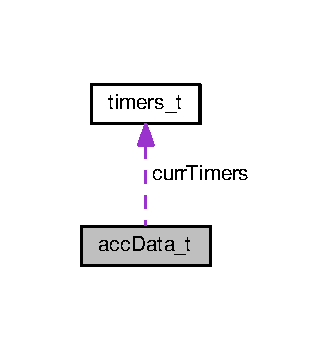
\includegraphics[width=160pt]{structaccData__t__coll__graph}
\end{center}
\end{figure}
\subsection*{Public Attributes}
\begin{DoxyCompactItemize}
\item 
\mbox{\Hypertarget{structaccData__t_a859abfd6c5404dced9d7a97c47c387fc}\label{structaccData__t_a859abfd6c5404dced9d7a97c47c387fc}} 
long double {\bfseries rate}
\item 
\mbox{\Hypertarget{structaccData__t_aba708e064c9e6733c3dff480d95344ed}\label{structaccData__t_aba708e064c9e6733c3dff480d95344ed}} 
\hyperlink{structtimers__t}{timers\+\_\+t} {\bfseries curr\+Timers} \mbox{[}sizeof(timers)/sizeof(timers\mbox{[}0\mbox{]})\mbox{]}
\item 
\mbox{\Hypertarget{structaccData__t_ab78550adb7a688c78ef8995de5b89bff}\label{structaccData__t_ab78550adb7a688c78ef8995de5b89bff}} 
int {\bfseries priority}
\end{DoxyCompactItemize}


The documentation for this struct was generated from the following files\+:\begin{DoxyCompactItemize}
\item 
proc\+\_\+modules/\hyperlink{htb_8cpp}{htb.\+cpp}\item 
proc\+\_\+modules/tbf.\+cpp\end{DoxyCompactItemize}

\hypertarget{structaction__t}{}\section{action\+\_\+t Struct Reference}
\label{structaction__t}\index{action\+\_\+t@{action\+\_\+t}}


F\+I\+X\+ME document!  




{\ttfamily \#include $<$Rule.\+h$>$}



Collaboration diagram for action\+\_\+t\+:
\nopagebreak
\begin{figure}[H]
\begin{center}
\leavevmode
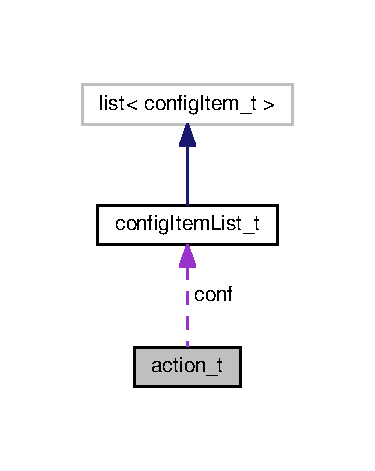
\includegraphics[width=180pt]{structaction__t__coll__graph}
\end{center}
\end{figure}
\subsection*{Public Attributes}
\begin{DoxyCompactItemize}
\item 
\mbox{\Hypertarget{structaction__t_af3cabd7053cd8b8b10ca26ac6e606b12}\label{structaction__t_af3cabd7053cd8b8b10ca26ac6e606b12}} 
string {\bfseries name}
\item 
\mbox{\Hypertarget{structaction__t_a615e1166fdee9eb36cbb2f421d6ef9cf}\label{structaction__t_a615e1166fdee9eb36cbb2f421d6ef9cf}} 
\hyperlink{classconfigItemList__t}{config\+Item\+List\+\_\+t} {\bfseries conf}
\end{DoxyCompactItemize}


\subsection{Detailed Description}
F\+I\+X\+ME document! 

The documentation for this struct was generated from the following file\+:\begin{DoxyCompactItemize}
\item 
include/\hyperlink{Rule_8h}{Rule.\+h}\end{DoxyCompactItemize}

\hypertarget{structActionModule__t}{}\section{Action\+Module\+\_\+t Struct Reference}
\label{structActionModule__t}\index{Action\+Module\+\_\+t@{Action\+Module\+\_\+t}}


struct that stores data for a loaded dynamic library  




{\ttfamily \#include $<$Module\+Loader.\+h$>$}



Collaboration diagram for Action\+Module\+\_\+t\+:
\nopagebreak
\begin{figure}[H]
\begin{center}
\leavevmode
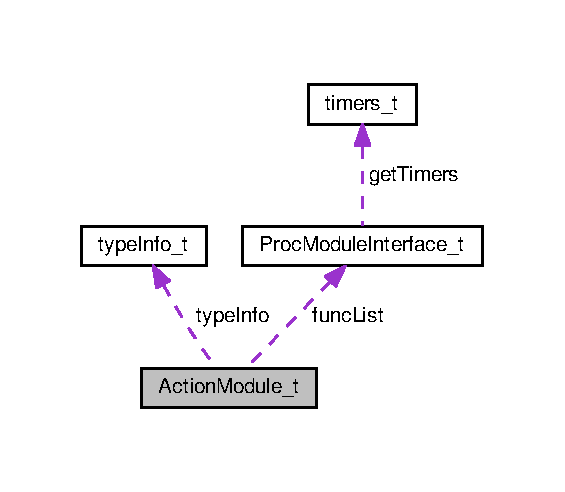
\includegraphics[width=271pt]{structActionModule__t__coll__graph}
\end{center}
\end{figure}
\subsection*{Public Attributes}
\begin{DoxyCompactItemize}
\item 
void $\ast$ \hyperlink{structActionModule__t_a94e6e256f50f4348101c7a9fb442b4b7}{libhandle}
\begin{DoxyCompactList}\small\item\em $<$ library handle from dlopen call \end{DoxyCompactList}\item 
\mbox{\Hypertarget{structActionModule__t_a1f9db14fee22694497154dfb3e6cb08a}\label{structActionModule__t_a1f9db14fee22694497154dfb3e6cb08a}} 
\hyperlink{structProcModuleInterface__t}{Proc\+Module\+Interface\+\_\+t} $\ast$ \hyperlink{structActionModule__t_a1f9db14fee22694497154dfb3e6cb08a}{func\+List}
\begin{DoxyCompactList}\small\item\em runtime type information list \end{DoxyCompactList}\item 
\mbox{\Hypertarget{structActionModule__t_af7980386654dffc270e2c654e08c84d7}\label{structActionModule__t_af7980386654dffc270e2c654e08c84d7}} 
\hyperlink{structtypeInfo__t}{type\+Info\+\_\+t} $\ast$ {\bfseries type\+Info}
\item 
\mbox{\Hypertarget{structActionModule__t_ad44b68b4bc09f4aa4a4cb6348fab449e}\label{structActionModule__t_ad44b68b4bc09f4aa4a4cb6348fab449e}} 
string \hyperlink{structActionModule__t_ad44b68b4bc09f4aa4a4cb6348fab449e}{name}
\begin{DoxyCompactList}\small\item\em name supplied by module \end{DoxyCompactList}\item 
\mbox{\Hypertarget{structActionModule__t_abf46b1d8d1c8101e30a3ea22420c61f5}\label{structActionModule__t_abf46b1d8d1c8101e30a3ea22420c61f5}} 
int \hyperlink{structActionModule__t_abf46b1d8d1c8101e30a3ea22420c61f5}{uid}
\begin{DoxyCompactList}\small\item\em unique id number supplied by module \end{DoxyCompactList}\item 
\mbox{\Hypertarget{structActionModule__t_a0ce7424ee92422bc9533fae56021fcfe}\label{structActionModule__t_a0ce7424ee92422bc9533fae56021fcfe}} 
int \hyperlink{structActionModule__t_a0ce7424ee92422bc9533fae56021fcfe}{ref}
\begin{DoxyCompactList}\small\item\em reference (link) counter \end{DoxyCompactList}\end{DoxyCompactItemize}


\subsection{Detailed Description}
struct that stores data for a loaded dynamic library 

this struct is used by a \hyperlink{classModuleLoader}{Module\+Loader} object to store information about a dynamically loaded library 

\subsection{Member Data Documentation}
\mbox{\Hypertarget{structActionModule__t_a94e6e256f50f4348101c7a9fb442b4b7}\label{structActionModule__t_a94e6e256f50f4348101c7a9fb442b4b7}} 
\index{Action\+Module\+\_\+t@{Action\+Module\+\_\+t}!libhandle@{libhandle}}
\index{libhandle@{libhandle}!Action\+Module\+\_\+t@{Action\+Module\+\_\+t}}
\subsubsection{\texorpdfstring{libhandle}{libhandle}}
{\footnotesize\ttfamily void$\ast$ Action\+Module\+\_\+t\+::libhandle}



$<$ library handle from dlopen call 

struct of functions pointers for library 

The documentation for this struct was generated from the following file\+:\begin{DoxyCompactItemize}
\item 
include/\hyperlink{ModuleLoader_8h}{Module\+Loader.\+h}\end{DoxyCompactItemize}

\hypertarget{classActivateRulesEvent}{}\section{Activate\+Rules\+Event Class Reference}
\label{classActivateRulesEvent}\index{Activate\+Rules\+Event@{Activate\+Rules\+Event}}


Inheritance diagram for Activate\+Rules\+Event\+:
\nopagebreak
\begin{figure}[H]
\begin{center}
\leavevmode
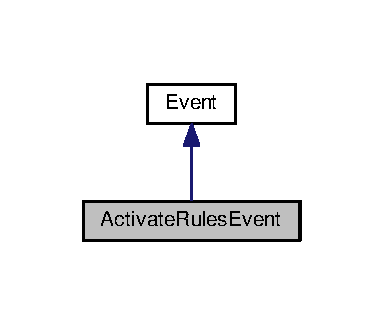
\includegraphics[width=184pt]{classActivateRulesEvent__inherit__graph}
\end{center}
\end{figure}


Collaboration diagram for Activate\+Rules\+Event\+:
\nopagebreak
\begin{figure}[H]
\begin{center}
\leavevmode
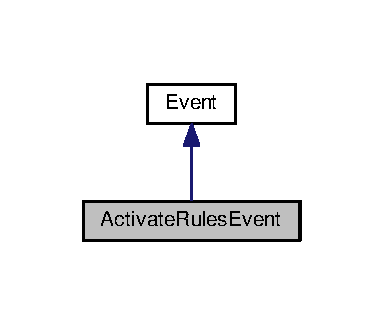
\includegraphics[width=184pt]{classActivateRulesEvent__coll__graph}
\end{center}
\end{figure}
\subsection*{Public Member Functions}
\begin{DoxyCompactItemize}
\item 
\mbox{\Hypertarget{classActivateRulesEvent_a4f746fa6b733d0ae6cbbcec60326a131}\label{classActivateRulesEvent_a4f746fa6b733d0ae6cbbcec60326a131}} 
{\bfseries Activate\+Rules\+Event} (struct timeval time, \hyperlink{RuleFileParser_8h_a7d5bb94bb17a8a1d92db2a89a0cc96d1}{rule\+D\+B\+\_\+t} \&r)
\item 
\mbox{\Hypertarget{classActivateRulesEvent_a2a5b8706ab54a60cbda9ce744f6cb542}\label{classActivateRulesEvent_a2a5b8706ab54a60cbda9ce744f6cb542}} 
{\bfseries Activate\+Rules\+Event} (time\+\_\+t offs\+\_\+sec, \hyperlink{RuleFileParser_8h_a7d5bb94bb17a8a1d92db2a89a0cc96d1}{rule\+D\+B\+\_\+t} \&r)
\item 
\mbox{\Hypertarget{classActivateRulesEvent_ab2a1e2d006b42902eb43952afd718e7c}\label{classActivateRulesEvent_ab2a1e2d006b42902eb43952afd718e7c}} 
{\bfseries Activate\+Rules\+Event} (\hyperlink{RuleFileParser_8h_a7d5bb94bb17a8a1d92db2a89a0cc96d1}{rule\+D\+B\+\_\+t} \&r)
\item 
\mbox{\Hypertarget{classActivateRulesEvent_abcf3b37831f1825f012ebe29c6013eb5}\label{classActivateRulesEvent_abcf3b37831f1825f012ebe29c6013eb5}} 
\hyperlink{RuleFileParser_8h_a7d5bb94bb17a8a1d92db2a89a0cc96d1}{rule\+D\+B\+\_\+t} $\ast$ {\bfseries get\+Rules} ()
\item 
\mbox{\Hypertarget{classActivateRulesEvent_ad6d8ae01bf7b38a90a05ac4eb6de94a4}\label{classActivateRulesEvent_ad6d8ae01bf7b38a90a05ac4eb6de94a4}} 
int \hyperlink{classActivateRulesEvent_ad6d8ae01bf7b38a90a05ac4eb6de94a4}{delete\+Rule} (int uid)
\begin{DoxyCompactList}\small\item\em delete rules stored in this event \end{DoxyCompactList}\end{DoxyCompactItemize}


The documentation for this class was generated from the following file\+:\begin{DoxyCompactItemize}
\item 
include/\hyperlink{Event_8h}{Event.\+h}\end{DoxyCompactItemize}

\hypertarget{classAddRulesCtrlEvent}{}\section{Add\+Rules\+Ctrl\+Event Class Reference}
\label{classAddRulesCtrlEvent}\index{Add\+Rules\+Ctrl\+Event@{Add\+Rules\+Ctrl\+Event}}


Inheritance diagram for Add\+Rules\+Ctrl\+Event\+:
\nopagebreak
\begin{figure}[H]
\begin{center}
\leavevmode
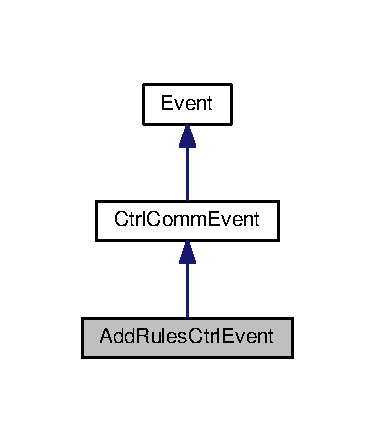
\includegraphics[width=180pt]{classAddRulesCtrlEvent__inherit__graph}
\end{center}
\end{figure}


Collaboration diagram for Add\+Rules\+Ctrl\+Event\+:
\nopagebreak
\begin{figure}[H]
\begin{center}
\leavevmode
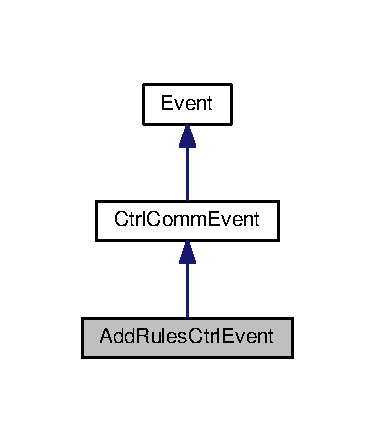
\includegraphics[width=180pt]{classAddRulesCtrlEvent__coll__graph}
\end{center}
\end{figure}
\subsection*{Public Member Functions}
\begin{DoxyCompactItemize}
\item 
\mbox{\Hypertarget{classAddRulesCtrlEvent_a5af5ac4b6ff5fda869dae033adc268e9}\label{classAddRulesCtrlEvent_a5af5ac4b6ff5fda869dae033adc268e9}} 
{\bfseries Add\+Rules\+Ctrl\+Event} (char $\ast$b, int l, int mapi=0)
\item 
\mbox{\Hypertarget{classAddRulesCtrlEvent_a9f79d6aa3898d5eb9c326b21fb4d3679}\label{classAddRulesCtrlEvent_a9f79d6aa3898d5eb9c326b21fb4d3679}} 
int {\bfseries is\+M\+A\+PI} ()
\item 
\mbox{\Hypertarget{classAddRulesCtrlEvent_a3b3b81319eed1706b8fb33249a5ec673}\label{classAddRulesCtrlEvent_a3b3b81319eed1706b8fb33249a5ec673}} 
char $\ast$ {\bfseries get\+Buf} ()
\item 
\mbox{\Hypertarget{classAddRulesCtrlEvent_a5988f3ea086722297af44c09d7aa300d}\label{classAddRulesCtrlEvent_a5988f3ea086722297af44c09d7aa300d}} 
int {\bfseries get\+Len} ()
\end{DoxyCompactItemize}


The documentation for this class was generated from the following file\+:\begin{DoxyCompactItemize}
\item 
include/\hyperlink{Event_8h}{Event.\+h}\end{DoxyCompactItemize}

\hypertarget{classAddRulesEvent}{}\section{Add\+Rules\+Event Class Reference}
\label{classAddRulesEvent}\index{Add\+Rules\+Event@{Add\+Rules\+Event}}


Inheritance diagram for Add\+Rules\+Event\+:
\nopagebreak
\begin{figure}[H]
\begin{center}
\leavevmode
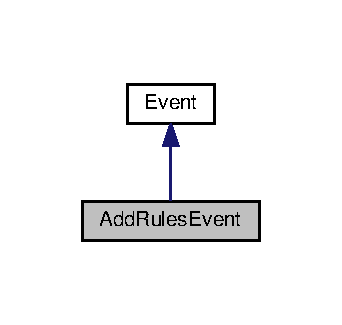
\includegraphics[width=164pt]{classAddRulesEvent__inherit__graph}
\end{center}
\end{figure}


Collaboration diagram for Add\+Rules\+Event\+:
\nopagebreak
\begin{figure}[H]
\begin{center}
\leavevmode
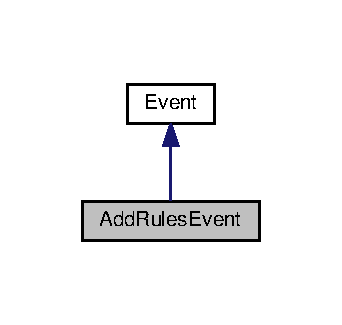
\includegraphics[width=164pt]{classAddRulesEvent__coll__graph}
\end{center}
\end{figure}
\subsection*{Public Member Functions}
\begin{DoxyCompactItemize}
\item 
\mbox{\Hypertarget{classAddRulesEvent_a6d3283dfa65c6bacd49d94fcb891b206}\label{classAddRulesEvent_a6d3283dfa65c6bacd49d94fcb891b206}} 
{\bfseries Add\+Rules\+Event} (string fname, int mapi=0)
\item 
\mbox{\Hypertarget{classAddRulesEvent_a139cf1cfd341da0a1b2dd377416fbf80}\label{classAddRulesEvent_a139cf1cfd341da0a1b2dd377416fbf80}} 
string {\bfseries get\+File\+Name} ()
\end{DoxyCompactItemize}


The documentation for this class was generated from the following file\+:\begin{DoxyCompactItemize}
\item 
include/\hyperlink{Event_8h}{Event.\+h}\end{DoxyCompactItemize}

\hypertarget{structcommandLineArg__t}{}\section{command\+Line\+Arg\+\_\+t Struct Reference}
\label{structcommandLineArg__t}\index{command\+Line\+Arg\+\_\+t@{command\+Line\+Arg\+\_\+t}}


command line arg  




{\ttfamily \#include $<$Command\+Line\+Args.\+h$>$}

\subsection*{Public Attributes}
\begin{DoxyCompactItemize}
\item 
\mbox{\Hypertarget{structcommandLineArg__t_a3db58af8143edf6cdee0c6af90c02bb4}\label{structcommandLineArg__t_a3db58af8143edf6cdee0c6af90c02bb4}} 
int \hyperlink{structcommandLineArg__t_a3db58af8143edf6cdee0c6af90c02bb4}{flag}
\begin{DoxyCompactList}\small\item\em is flag \end{DoxyCompactList}\item 
\mbox{\Hypertarget{structcommandLineArg__t_a71b0eabcff73ed6f189119de3e179f1e}\label{structcommandLineArg__t_a71b0eabcff73ed6f189119de3e179f1e}} 
string \hyperlink{structcommandLineArg__t_a71b0eabcff73ed6f189119de3e179f1e}{param}
\begin{DoxyCompactList}\small\item\em parameter(s) \end{DoxyCompactList}\item 
\mbox{\Hypertarget{structcommandLineArg__t_ab8d597b3f07f9fe0d09bacba036cb1a6}\label{structcommandLineArg__t_ab8d597b3f07f9fe0d09bacba036cb1a6}} 
string \hyperlink{structcommandLineArg__t_ab8d597b3f07f9fe0d09bacba036cb1a6}{help}
\begin{DoxyCompactList}\small\item\em help text for the argument \end{DoxyCompactList}\item 
\mbox{\Hypertarget{structcommandLineArg__t_ace90133da5e170fa09b6d1220dbaf9f7}\label{structcommandLineArg__t_ace90133da5e170fa09b6d1220dbaf9f7}} 
string \hyperlink{structcommandLineArg__t_ace90133da5e170fa09b6d1220dbaf9f7}{name}
\begin{DoxyCompactList}\small\item\em name of the argument \end{DoxyCompactList}\item 
\mbox{\Hypertarget{structcommandLineArg__t_af9f59b1b39bbb0462228f3fb38e88b10}\label{structcommandLineArg__t_af9f59b1b39bbb0462228f3fb38e88b10}} 
string \hyperlink{structcommandLineArg__t_af9f59b1b39bbb0462228f3fb38e88b10}{group}
\begin{DoxyCompactList}\small\item\em group of the argument \end{DoxyCompactList}\item 
\mbox{\Hypertarget{structcommandLineArg__t_a7fbd7b4bc8e545801a8551a80214e7c9}\label{structcommandLineArg__t_a7fbd7b4bc8e545801a8551a80214e7c9}} 
string \hyperlink{structcommandLineArg__t_a7fbd7b4bc8e545801a8551a80214e7c9}{longname}
\begin{DoxyCompactList}\small\item\em longname of the argument \end{DoxyCompactList}\end{DoxyCompactItemize}


\subsection{Detailed Description}
command line arg 

The documentation for this struct was generated from the following file\+:\begin{DoxyCompactItemize}
\item 
include/\hyperlink{CommandLineArgs_8h}{Command\+Line\+Args.\+h}\end{DoxyCompactItemize}

\hypertarget{classCommandLineArgs}{}\section{Command\+Line\+Args Class Reference}
\label{classCommandLineArgs}\index{Command\+Line\+Args@{Command\+Line\+Args}}
\subsection*{Public Member Functions}
\begin{DoxyCompactItemize}
\item 
\mbox{\Hypertarget{classCommandLineArgs_adf3473a1701ad5b5945b1ad5fbe0db9b}\label{classCommandLineArgs_adf3473a1701ad5b5945b1ad5fbe0db9b}} 
\hyperlink{classCommandLineArgs_adf3473a1701ad5b5945b1ad5fbe0db9b}{Command\+Line\+Args} ()
\begin{DoxyCompactList}\small\item\em construct a new \hyperlink{classCommandLineArgs}{Command\+Line\+Args} object \end{DoxyCompactList}\item 
\mbox{\Hypertarget{classCommandLineArgs_a11bbea9577ad97fa8ccb024a9869e4c5}\label{classCommandLineArgs_a11bbea9577ad97fa8ccb024a9869e4c5}} 
void \hyperlink{classCommandLineArgs_a11bbea9577ad97fa8ccb024a9869e4c5}{add} (char opt, string name, string param=\char`\"{}\char`\"{}, string help=\char`\"{}\char`\"{}, string group=\char`\"{}\char`\"{}, string longname=\char`\"{}\char`\"{})
\begin{DoxyCompactList}\small\item\em add a command line argument expecting a value \end{DoxyCompactList}\item 
\mbox{\Hypertarget{classCommandLineArgs_aae885cc296df2013e8e30eeba30d1483}\label{classCommandLineArgs_aae885cc296df2013e8e30eeba30d1483}} 
void \hyperlink{classCommandLineArgs_aae885cc296df2013e8e30eeba30d1483}{add\+Flag} (char opt, string name, string help=\char`\"{}\char`\"{}, string group=\char`\"{}\char`\"{}, string longname=\char`\"{}\char`\"{})
\begin{DoxyCompactList}\small\item\em add a command line argument flag (yes/no) \end{DoxyCompactList}\item 
\mbox{\Hypertarget{classCommandLineArgs_a673c25d7b7c3cbb3d243b5ee4f65f76c}\label{classCommandLineArgs_a673c25d7b7c3cbb3d243b5ee4f65f76c}} 
string \hyperlink{classCommandLineArgs_a673c25d7b7c3cbb3d243b5ee4f65f76c}{get\+Arg\+Value} (char opt)
\begin{DoxyCompactList}\small\item\em get the value for an argument \end{DoxyCompactList}\item 
\mbox{\Hypertarget{classCommandLineArgs_a26e8d3a0e201d0c2808ef212a7a6e6f8}\label{classCommandLineArgs_a26e8d3a0e201d0c2808ef212a7a6e6f8}} 
int \hyperlink{classCommandLineArgs_a26e8d3a0e201d0c2808ef212a7a6e6f8}{parse\+Args} (int argc, char $\ast$argv\mbox{[}$\,$\mbox{]})
\begin{DoxyCompactList}\small\item\em parse the command line args supplied to main \end{DoxyCompactList}\item 
\mbox{\Hypertarget{classCommandLineArgs_a2f9280db1c9b8cd7644537c111ee0787}\label{classCommandLineArgs_a2f9280db1c9b8cd7644537c111ee0787}} 
\hyperlink{CommandLineArgs_8h_a092e791e8505f700f627414f125dcd6e}{command\+Line\+Arg\+Val\+List\+\_\+t} $\ast$ \hyperlink{classCommandLineArgs_a2f9280db1c9b8cd7644537c111ee0787}{get\+Arg\+Vals} ()
\begin{DoxyCompactList}\small\item\em get pointer to argument values \end{DoxyCompactList}\item 
\mbox{\Hypertarget{classCommandLineArgs_ad04d8c3fa544cd7f3a070a181675ae71}\label{classCommandLineArgs_ad04d8c3fa544cd7f3a070a181675ae71}} 
\hyperlink{CommandLineArgs_8h_aaee5f0d903dd3ebb586b68e0cd4d5594}{command\+Line\+Arg\+List\+\_\+t} $\ast$ \hyperlink{classCommandLineArgs_ad04d8c3fa544cd7f3a070a181675ae71}{get\+Arg\+List} ()
\begin{DoxyCompactList}\small\item\em get pointer to argument definition list \end{DoxyCompactList}\item 
\mbox{\Hypertarget{classCommandLineArgs_acb1dd9919009b2a61a9416efd9583d7f}\label{classCommandLineArgs_acb1dd9919009b2a61a9416efd9583d7f}} 
string \hyperlink{classCommandLineArgs_acb1dd9919009b2a61a9416efd9583d7f}{get\+Usage} ()
\begin{DoxyCompactList}\small\item\em get usage string (is build from options description) \end{DoxyCompactList}\end{DoxyCompactItemize}


The documentation for this class was generated from the following files\+:\begin{DoxyCompactItemize}
\item 
include/\hyperlink{CommandLineArgs_8h}{Command\+Line\+Args.\+h}\item 
src/Command\+Line\+Args.\+cpp\end{DoxyCompactItemize}

\hypertarget{structcondItem__t}{}\section{cond\+Item\+\_\+t Struct Reference}
\label{structcondItem__t}\index{cond\+Item\+\_\+t@{cond\+Item\+\_\+t}}


conditional item  




{\ttfamily \#include $<$Filter\+Def\+Parser.\+h$>$}



Collaboration diagram for cond\+Item\+\_\+t\+:
\nopagebreak
\begin{figure}[H]
\begin{center}
\leavevmode
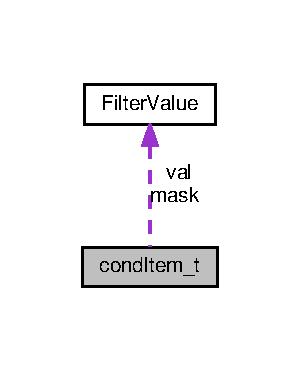
\includegraphics[width=144pt]{structcondItem__t__coll__graph}
\end{center}
\end{figure}
\subsection*{Public Attributes}
\begin{DoxyCompactItemize}
\item 
\mbox{\Hypertarget{structcondItem__t_a22c02ebadfc28c0a00540462cd975371}\label{structcondItem__t_a22c02ebadfc28c0a00540462cd975371}} 
string {\bfseries name}
\item 
\mbox{\Hypertarget{structcondItem__t_ab3c9ea5bf5fb5ae0638bc3fdacdbf5d7}\label{structcondItem__t_ab3c9ea5bf5fb5ae0638bc3fdacdbf5d7}} 
\hyperlink{classFilterValue}{Filter\+Value} {\bfseries mask}
\item 
\mbox{\Hypertarget{structcondItem__t_a164a56089a136e81be945af1f6a8f6e0}\label{structcondItem__t_a164a56089a136e81be945af1f6a8f6e0}} 
\hyperlink{classFilterValue}{Filter\+Value} {\bfseries val}
\end{DoxyCompactItemize}


\subsection{Detailed Description}
conditional item 

The documentation for this struct was generated from the following file\+:\begin{DoxyCompactItemize}
\item 
include/Filter\+Def\+Parser.\+h\end{DoxyCompactItemize}

\hypertarget{structconfigADItem__t}{}\section{config\+A\+D\+Item\+\_\+t Struct Reference}
\label{structconfigADItem__t}\index{config\+A\+D\+Item\+\_\+t@{config\+A\+D\+Item\+\_\+t}}


access configuration item  




{\ttfamily \#include $<$Config\+Parser.\+h$>$}

\subsection*{Public Attributes}
\begin{DoxyCompactItemize}
\item 
\mbox{\Hypertarget{structconfigADItem__t_a104792ad14ceeab63d264721f9f5bdff}\label{structconfigADItem__t_a104792ad14ceeab63d264721f9f5bdff}} 
ad\+\_\+t {\bfseries ad}
\item 
\mbox{\Hypertarget{structconfigADItem__t_a3656c6f32c167719777804aca5c1db36}\label{structconfigADItem__t_a3656c6f32c167719777804aca5c1db36}} 
string {\bfseries value}
\item 
\mbox{\Hypertarget{structconfigADItem__t_a0720d50a27c2b0dc48af7596627177f6}\label{structconfigADItem__t_a0720d50a27c2b0dc48af7596627177f6}} 
string {\bfseries type}
\item 
string \hyperlink{structconfigADItem__t_a8688b276c6fc46d46e771fc273e301ed}{resolve\+\_\+addr}
\end{DoxyCompactItemize}


\subsection{Detailed Description}
access configuration item 

\subsection{Member Data Documentation}
\mbox{\Hypertarget{structconfigADItem__t_a8688b276c6fc46d46e771fc273e301ed}\label{structconfigADItem__t_a8688b276c6fc46d46e771fc273e301ed}} 
\index{config\+A\+D\+Item\+\_\+t@{config\+A\+D\+Item\+\_\+t}!resolve\+\_\+addr@{resolve\+\_\+addr}}
\index{resolve\+\_\+addr@{resolve\+\_\+addr}!config\+A\+D\+Item\+\_\+t@{config\+A\+D\+Item\+\_\+t}}
\subsubsection{\texorpdfstring{resolve\+\_\+addr}{resolve\_addr}}
{\footnotesize\ttfamily string config\+A\+D\+Item\+\_\+t\+::resolve\+\_\+addr}

may contain IP address if host based item and value is valid IP address or host name 

The documentation for this struct was generated from the following file\+:\begin{DoxyCompactItemize}
\item 
include/Config\+Parser.\+h\end{DoxyCompactItemize}

\hypertarget{structconfigItem}{}\section{config\+Item Struct Reference}
\label{structconfigItem}\index{config\+Item@{config\+Item}}


configuration item  




{\ttfamily \#include $<$Config\+Parser.\+h$>$}

\subsection*{Public Attributes}
\begin{DoxyCompactItemize}
\item 
\mbox{\Hypertarget{structconfigItem_a8bd065514c64d606dc2c7b74f995eaf6}\label{structconfigItem_a8bd065514c64d606dc2c7b74f995eaf6}} 
string {\bfseries group}
\item 
\mbox{\Hypertarget{structconfigItem_a5777d37b02899012de8b8e9750054e2b}\label{structconfigItem_a5777d37b02899012de8b8e9750054e2b}} 
string {\bfseries module}
\item 
\mbox{\Hypertarget{structconfigItem_a53010d9f4f57d979a3798a28126d7d9d}\label{structconfigItem_a53010d9f4f57d979a3798a28126d7d9d}} 
string {\bfseries name}
\item 
\mbox{\Hypertarget{structconfigItem_afc9fecce2bdc20bd6a1d63785300c210}\label{structconfigItem_afc9fecce2bdc20bd6a1d63785300c210}} 
string {\bfseries value}
\item 
\mbox{\Hypertarget{structconfigItem_a36f596e7068403288accf722523cbbbf}\label{structconfigItem_a36f596e7068403288accf722523cbbbf}} 
string {\bfseries type}
\end{DoxyCompactItemize}


\subsection{Detailed Description}
configuration item 

The documentation for this struct was generated from the following file\+:\begin{DoxyCompactItemize}
\item 
include/Config\+Parser.\+h\end{DoxyCompactItemize}

\hypertarget{classconfigItemList__t}{}\section{config\+Item\+List\+\_\+t Class Reference}
\label{classconfigItemList__t}\index{config\+Item\+List\+\_\+t@{config\+Item\+List\+\_\+t}}


list of config items  




{\ttfamily \#include $<$Config\+Parser.\+h$>$}



Inheritance diagram for config\+Item\+List\+\_\+t\+:
\nopagebreak
\begin{figure}[H]
\begin{center}
\leavevmode
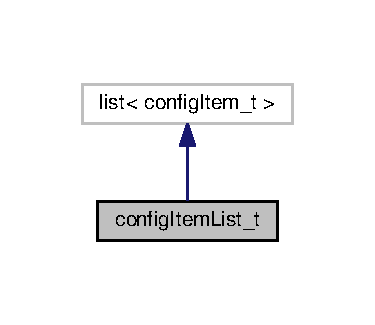
\includegraphics[width=180pt]{classconfigItemList__t__inherit__graph}
\end{center}
\end{figure}


Collaboration diagram for config\+Item\+List\+\_\+t\+:
\nopagebreak
\begin{figure}[H]
\begin{center}
\leavevmode
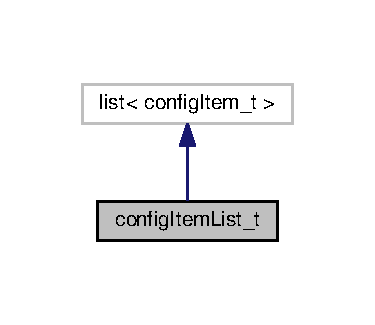
\includegraphics[width=180pt]{classconfigItemList__t__coll__graph}
\end{center}
\end{figure}
\subsection*{Public Member Functions}
\begin{DoxyCompactItemize}
\item 
\mbox{\Hypertarget{classconfigItemList__t_a85b9cc4dfb3d218b3da8678ebf319157}\label{classconfigItemList__t_a85b9cc4dfb3d218b3da8678ebf319157}} 
string {\bfseries get\+Value} (string name)
\end{DoxyCompactItemize}


\subsection{Detailed Description}
list of config items 

The documentation for this class was generated from the following files\+:\begin{DoxyCompactItemize}
\item 
include/Config\+Parser.\+h\item 
src/Config\+Parser.\+cpp\end{DoxyCompactItemize}

\hypertarget{classConfigManager}{}\section{Config\+Manager Class Reference}
\label{classConfigManager}\index{Config\+Manager@{Config\+Manager}}
\subsection*{Public Member Functions}
\begin{DoxyCompactItemize}
\item 
\hyperlink{classConfigManager_a1676cfe00c3b4e794fdc258d935347a1}{Config\+Manager} (string filename, string binary)
\item 
\mbox{\Hypertarget{classConfigManager_a7fa65fdff98bdd5bbbf72196bd9ccf17}\label{classConfigManager_a7fa65fdff98bdd5bbbf72196bd9ccf17}} 
\hyperlink{classConfigManager_a7fa65fdff98bdd5bbbf72196bd9ccf17}{$\sim$\+Config\+Manager} ()
\begin{DoxyCompactList}\small\item\em destroys a \hyperlink{classConfigManager}{Config\+Manager} object \end{DoxyCompactList}\item 
void \hyperlink{classConfigManager_af4ffb3955f672a1dd0fb1db39d231c2a}{reread} (const string fname)
\begin{DoxyCompactList}\small\item\em reads config strings from file into object\textquotesingle{}s string table \end{DoxyCompactList}\item 
string \hyperlink{classConfigManager_ae6ad7a04fbbc00fa5f5297daed17e4df}{get\+Value} (string name, string group=\char`\"{}\char`\"{}, string module=\char`\"{}\char`\"{})
\begin{DoxyCompactList}\small\item\em get configured item\textquotesingle{}s value \end{DoxyCompactList}\item 
\hyperlink{structconfigItem}{config\+Item\+\_\+t} $\ast$ \hyperlink{classConfigManager_a3cdebcc0fc8ce6148943963ba64ba342}{get\+Item} (string name, string group=\char`\"{}\char`\"{}, string module=\char`\"{}\char`\"{})
\begin{DoxyCompactList}\small\item\em get a pointer to an item definition \end{DoxyCompactList}\item 
\mbox{\Hypertarget{classConfigManager_acd83de4b0766edde05c4b3f93afedccc}\label{classConfigManager_acd83de4b0766edde05c4b3f93afedccc}} 
\hyperlink{classconfigItemList__t}{config\+Item\+List\+\_\+t} \hyperlink{classConfigManager_acd83de4b0766edde05c4b3f93afedccc}{get\+Items} (string group, string module=\char`\"{}\char`\"{})
\begin{DoxyCompactList}\small\item\em get all items for the specified module \end{DoxyCompactList}\item 
int \hyperlink{classConfigManager_ae065527722202c0c34d2e775774e27b0}{is\+Configured} (string name, string group=\char`\"{}\char`\"{}, string module=\char`\"{}\char`\"{})
\begin{DoxyCompactList}\small\item\em query if item is configured at all \end{DoxyCompactList}\item 
int \hyperlink{classConfigManager_af39ad88f6a49f537c1660aa186f4f4eb}{is\+True} (string name, string group=\char`\"{}\char`\"{}, string module=\char`\"{}\char`\"{})
\begin{DoxyCompactList}\small\item\em check if item is configured to be true \end{DoxyCompactList}\item 
int \hyperlink{classConfigManager_a217e3864c2c7afe3a340df6405d56a55}{is\+False} (string name, string group=\char`\"{}\char`\"{}, string module=\char`\"{}\char`\"{})
\begin{DoxyCompactList}\small\item\em check if item is configured to be false \end{DoxyCompactList}\item 
void \hyperlink{classConfigManager_a63619a561041c0d5e11c7751b5d999e8}{set\+Item} (string name, string value, string group=\char`\"{}\char`\"{}, string module=\char`\"{}\char`\"{})
\begin{DoxyCompactList}\small\item\em set configured item\textquotesingle{}s value to a specified string \end{DoxyCompactList}\item 
\mbox{\Hypertarget{classConfigManager_a806bb8edd47dcdd24633a057f5952502}\label{classConfigManager_a806bb8edd47dcdd24633a057f5952502}} 
config\+A\+D\+List\+\_\+t \& \hyperlink{classConfigManager_a806bb8edd47dcdd24633a057f5952502}{get\+Access\+List} ()
\begin{DoxyCompactList}\small\item\em get a pointer to the access list \end{DoxyCompactList}\item 
void \hyperlink{classConfigManager_aa8cff61a46545834f88553cfb00beefd}{merge\+Args} (\hyperlink{CommandLineArgs_8h_aaee5f0d903dd3ebb586b68e0cd4d5594}{command\+Line\+Arg\+List\+\_\+t} $\ast$args, \hyperlink{CommandLineArgs_8h_a092e791e8505f700f627414f125dcd6e}{command\+Line\+Arg\+Val\+List\+\_\+t} $\ast$arg\+Vals)
\item 
\mbox{\Hypertarget{classConfigManager_abc8efd3c2dd742b3a5fc461eab9d32fc}\label{classConfigManager_abc8efd3c2dd742b3a5fc461eab9d32fc}} 
void \hyperlink{classConfigManager_abc8efd3c2dd742b3a5fc461eab9d32fc}{dump} (ostream \&os)
\begin{DoxyCompactList}\small\item\em dump object (list of configured items) \end{DoxyCompactList}\end{DoxyCompactItemize}
\subsection*{Static Public Member Functions}
\begin{DoxyCompactItemize}
\item 
\mbox{\Hypertarget{classConfigManager_a64a3c942890179cba28b86e07a3805a8}\label{classConfigManager_a64a3c942890179cba28b86e07a3805a8}} 
static \hyperlink{structconfigParam__t}{config\+Param\+\_\+t} $\ast$ \hyperlink{classConfigManager_a64a3c942890179cba28b86e07a3805a8}{get\+Param\+List} (\hyperlink{classconfigItemList__t}{config\+Item\+List\+\_\+t} \&list)
\begin{DoxyCompactList}\small\item\em create a C-\/style param list for the proc modules \end{DoxyCompactList}\item 
static \hyperlink{structconfigParam__t}{config\+Param\+\_\+t} $\ast$ \hyperlink{classConfigManager_af019debefe1c024dc6e222fd0cbd63ef}{merge\+Param\+List} (\hyperlink{structconfigParam__t}{config\+Param\+\_\+t} $\ast$list\+\_\+a, \hyperlink{structconfigParam__t}{config\+Param\+\_\+t} $\ast$list\+\_\+b)
\end{DoxyCompactItemize}


\subsection{Constructor \& Destructor Documentation}
\mbox{\Hypertarget{classConfigManager_a1676cfe00c3b4e794fdc258d935347a1}\label{classConfigManager_a1676cfe00c3b4e794fdc258d935347a1}} 
\index{Config\+Manager@{Config\+Manager}!Config\+Manager@{Config\+Manager}}
\index{Config\+Manager@{Config\+Manager}!Config\+Manager@{Config\+Manager}}
\subsubsection{\texorpdfstring{Config\+Manager()}{ConfigManager()}}
{\footnotesize\ttfamily Config\+Manager\+::\+Config\+Manager (\begin{DoxyParamCaption}\item[{string}]{filename,  }\item[{string}]{binary }\end{DoxyParamCaption})}

creates and initializes a \hyperlink{classConfigManager}{Config\+Manager} \begin{DoxyItemize}
\item {\ttfamily filename} -\/ name of config file \item {\ttfamily binary} -\/ location of binary file, i.\+e. argv\mbox{[}0\mbox{]} \end{DoxyItemize}


\subsection{Member Function Documentation}
\mbox{\Hypertarget{classConfigManager_a3cdebcc0fc8ce6148943963ba64ba342}\label{classConfigManager_a3cdebcc0fc8ce6148943963ba64ba342}} 
\index{Config\+Manager@{Config\+Manager}!get\+Item@{get\+Item}}
\index{get\+Item@{get\+Item}!Config\+Manager@{Config\+Manager}}
\subsubsection{\texorpdfstring{get\+Item()}{getItem()}}
{\footnotesize\ttfamily \hyperlink{structconfigItem}{config\+Item\+\_\+t} $\ast$ Config\+Manager\+::get\+Item (\begin{DoxyParamCaption}\item[{string}]{name,  }\item[{string}]{group = {\ttfamily \char`\"{}\char`\"{}},  }\item[{string}]{module = {\ttfamily \char`\"{}\char`\"{}} }\end{DoxyParamCaption})}



get a pointer to an item definition 

\begin{DoxyItemize}
\item {\ttfamily name} -\/ name of the item \begin{DoxyReturn}{Returns}
a pointer to the item definition or N\+U\+LL if item is not set 
\end{DoxyReturn}
\end{DoxyItemize}
\mbox{\Hypertarget{classConfigManager_ae6ad7a04fbbc00fa5f5297daed17e4df}\label{classConfigManager_ae6ad7a04fbbc00fa5f5297daed17e4df}} 
\index{Config\+Manager@{Config\+Manager}!get\+Value@{get\+Value}}
\index{get\+Value@{get\+Value}!Config\+Manager@{Config\+Manager}}
\subsubsection{\texorpdfstring{get\+Value()}{getValue()}}
{\footnotesize\ttfamily string Config\+Manager\+::get\+Value (\begin{DoxyParamCaption}\item[{string}]{name,  }\item[{string}]{group = {\ttfamily \char`\"{}\char`\"{}},  }\item[{string}]{module = {\ttfamily \char`\"{}\char`\"{}} }\end{DoxyParamCaption})}



get configured item\textquotesingle{}s value 

\begin{DoxyItemize}
\item {\ttfamily name} -\/ name of the item \begin{DoxyReturn}{Returns}
the value for the queried item or \char`\"{}\char`\"{} if item is not set 
\end{DoxyReturn}
\end{DoxyItemize}
\mbox{\Hypertarget{classConfigManager_ae065527722202c0c34d2e775774e27b0}\label{classConfigManager_ae065527722202c0c34d2e775774e27b0}} 
\index{Config\+Manager@{Config\+Manager}!is\+Configured@{is\+Configured}}
\index{is\+Configured@{is\+Configured}!Config\+Manager@{Config\+Manager}}
\subsubsection{\texorpdfstring{is\+Configured()}{isConfigured()}}
{\footnotesize\ttfamily int Config\+Manager\+::is\+Configured (\begin{DoxyParamCaption}\item[{string}]{name,  }\item[{string}]{group = {\ttfamily \char`\"{}\char`\"{}},  }\item[{string}]{module = {\ttfamily \char`\"{}\char`\"{}} }\end{DoxyParamCaption})}



query if item is configured at all 

\begin{DoxyItemize}
\item {\ttfamily name} -\/ name of queried item \begin{DoxyReturn}{Returns}
a value !=0 if item has been configured, else 0 
\end{DoxyReturn}
\end{DoxyItemize}
\mbox{\Hypertarget{classConfigManager_a217e3864c2c7afe3a340df6405d56a55}\label{classConfigManager_a217e3864c2c7afe3a340df6405d56a55}} 
\index{Config\+Manager@{Config\+Manager}!is\+False@{is\+False}}
\index{is\+False@{is\+False}!Config\+Manager@{Config\+Manager}}
\subsubsection{\texorpdfstring{is\+False()}{isFalse()}}
{\footnotesize\ttfamily int Config\+Manager\+::is\+False (\begin{DoxyParamCaption}\item[{string}]{name,  }\item[{string}]{group = {\ttfamily \char`\"{}\char`\"{}},  }\item[{string}]{module = {\ttfamily \char`\"{}\char`\"{}} }\end{DoxyParamCaption})}



check if item is configured to be false 

this will lookup the given item in the list of configured items and return true if the item is either set to be \textquotesingle{}0\textquotesingle{}, \textquotesingle{}false\textquotesingle{} or \textquotesingle{}no\textquotesingle{}. Items which are configured but do not have a value are considered false.

\begin{DoxyItemize}
\item {\ttfamily name} -\/ name of queried item \begin{DoxyReturn}{Returns}
a value !=0 if item is configured to one of \textquotesingle{}0\textquotesingle{},\textquotesingle{}false\textquotesingle{},\textquotesingle{}no\textquotesingle{} 
\end{DoxyReturn}
\end{DoxyItemize}
\mbox{\Hypertarget{classConfigManager_af39ad88f6a49f537c1660aa186f4f4eb}\label{classConfigManager_af39ad88f6a49f537c1660aa186f4f4eb}} 
\index{Config\+Manager@{Config\+Manager}!is\+True@{is\+True}}
\index{is\+True@{is\+True}!Config\+Manager@{Config\+Manager}}
\subsubsection{\texorpdfstring{is\+True()}{isTrue()}}
{\footnotesize\ttfamily int Config\+Manager\+::is\+True (\begin{DoxyParamCaption}\item[{string}]{name,  }\item[{string}]{group = {\ttfamily \char`\"{}\char`\"{}},  }\item[{string}]{module = {\ttfamily \char`\"{}\char`\"{}} }\end{DoxyParamCaption})}



check if item is configured to be true 

this will lookup the given item in the list of configured items and return true if the item is either set to be \textquotesingle{}1\textquotesingle{}, \textquotesingle{}true\textquotesingle{} or \textquotesingle{}yes\textquotesingle{}.

\begin{DoxyItemize}
\item {\ttfamily name} -\/ name of queried item \begin{DoxyReturn}{Returns}
a value !=0 if item is configured to one of \textquotesingle{}1\textquotesingle{},\textquotesingle{}true\textquotesingle{},\textquotesingle{}yes\textquotesingle{} or \textquotesingle{}\textquotesingle{} 
\end{DoxyReturn}
\end{DoxyItemize}
\mbox{\Hypertarget{classConfigManager_aa8cff61a46545834f88553cfb00beefd}\label{classConfigManager_aa8cff61a46545834f88553cfb00beefd}} 
\index{Config\+Manager@{Config\+Manager}!merge\+Args@{merge\+Args}}
\index{merge\+Args@{merge\+Args}!Config\+Manager@{Config\+Manager}}
\subsubsection{\texorpdfstring{merge\+Args()}{mergeArgs()}}
{\footnotesize\ttfamily void Config\+Manager\+::merge\+Args (\begin{DoxyParamCaption}\item[{\hyperlink{CommandLineArgs_8h_aaee5f0d903dd3ebb586b68e0cd4d5594}{command\+Line\+Arg\+List\+\_\+t} $\ast$}]{args,  }\item[{\hyperlink{CommandLineArgs_8h_a092e791e8505f700f627414f125dcd6e}{command\+Line\+Arg\+Val\+List\+\_\+t} $\ast$}]{arg\+Vals }\end{DoxyParamCaption})}

merge command line args into config database command line args overrule existing configuration \mbox{\Hypertarget{classConfigManager_af019debefe1c024dc6e222fd0cbd63ef}\label{classConfigManager_af019debefe1c024dc6e222fd0cbd63ef}} 
\index{Config\+Manager@{Config\+Manager}!merge\+Param\+List@{merge\+Param\+List}}
\index{merge\+Param\+List@{merge\+Param\+List}!Config\+Manager@{Config\+Manager}}
\subsubsection{\texorpdfstring{merge\+Param\+List()}{mergeParamList()}}
{\footnotesize\ttfamily \hyperlink{structconfigParam__t}{config\+Param\+\_\+t} $\ast$ Config\+Manager\+::merge\+Param\+List (\begin{DoxyParamCaption}\item[{\hyperlink{structconfigParam__t}{config\+Param\+\_\+t} $\ast$}]{list\+\_\+a,  }\item[{\hyperlink{structconfigParam__t}{config\+Param\+\_\+t} $\ast$}]{list\+\_\+b }\end{DoxyParamCaption})\hspace{0.3cm}{\ttfamily [static]}}

merge two C-\/style param list for the proc modules \mbox{\Hypertarget{classConfigManager_af4ffb3955f672a1dd0fb1db39d231c2a}\label{classConfigManager_af4ffb3955f672a1dd0fb1db39d231c2a}} 
\index{Config\+Manager@{Config\+Manager}!reread@{reread}}
\index{reread@{reread}!Config\+Manager@{Config\+Manager}}
\subsubsection{\texorpdfstring{reread()}{reread()}}
{\footnotesize\ttfamily void Config\+Manager\+::reread (\begin{DoxyParamCaption}\item[{const string}]{fname }\end{DoxyParamCaption})}



reads config strings from file into object\textquotesingle{}s string table 

if used more than once, new items and values will be added to those already set. Old items may be overwritten.

\begin{DoxyItemize}
\item {\ttfamily fname} -\/ name of file to read configuration from \end{DoxyItemize}
\mbox{\Hypertarget{classConfigManager_a63619a561041c0d5e11c7751b5d999e8}\label{classConfigManager_a63619a561041c0d5e11c7751b5d999e8}} 
\index{Config\+Manager@{Config\+Manager}!set\+Item@{set\+Item}}
\index{set\+Item@{set\+Item}!Config\+Manager@{Config\+Manager}}
\subsubsection{\texorpdfstring{set\+Item()}{setItem()}}
{\footnotesize\ttfamily void Config\+Manager\+::set\+Item (\begin{DoxyParamCaption}\item[{string}]{name,  }\item[{string}]{value,  }\item[{string}]{group = {\ttfamily \char`\"{}\char`\"{}},  }\item[{string}]{module = {\ttfamily \char`\"{}\char`\"{}} }\end{DoxyParamCaption})}



set configured item\textquotesingle{}s value to a specified string 

\begin{DoxyItemize}
\item {\ttfamily name} name of the item \item {\ttfamily value} string value to be set \item {\ttfamily group} group of the item (optional) \item {\ttfamily module} module of the item (optional) \end{DoxyItemize}


The documentation for this class was generated from the following files\+:\begin{DoxyCompactItemize}
\item 
include/\hyperlink{ConfigManager_8h}{Config\+Manager.\+h}\item 
src/Config\+Manager.\+cpp\end{DoxyCompactItemize}

\hypertarget{structconfigParam__t}{}\section{config\+Param\+\_\+t Struct Reference}
\label{structconfigParam__t}\index{config\+Param\+\_\+t@{config\+Param\+\_\+t}}
\subsection*{Public Attributes}
\begin{DoxyCompactItemize}
\item 
\mbox{\Hypertarget{structconfigParam__t_ab0dc86e40d7b2837ea0d765649ce450a}\label{structconfigParam__t_ab0dc86e40d7b2837ea0d765649ce450a}} 
char $\ast$ {\bfseries name}
\item 
\mbox{\Hypertarget{structconfigParam__t_a8b2e07217ec9db22113a25c6d43ff19d}\label{structconfigParam__t_a8b2e07217ec9db22113a25c6d43ff19d}} 
char $\ast$ {\bfseries value}
\end{DoxyCompactItemize}


The documentation for this struct was generated from the following file\+:\begin{DoxyCompactItemize}
\item 
include/\hyperlink{ProcModuleInterface_8h}{Proc\+Module\+Interface.\+h}\end{DoxyCompactItemize}

\hypertarget{classConfigParser}{}\section{Config\+Parser Class Reference}
\label{classConfigParser}\index{Config\+Parser@{Config\+Parser}}


Inheritance diagram for Config\+Parser\+:
\nopagebreak
\begin{figure}[H]
\begin{center}
\leavevmode
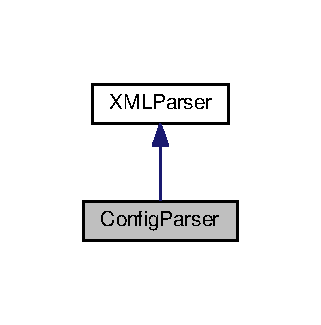
\includegraphics[width=154pt]{classConfigParser__inherit__graph}
\end{center}
\end{figure}


Collaboration diagram for Config\+Parser\+:
\nopagebreak
\begin{figure}[H]
\begin{center}
\leavevmode
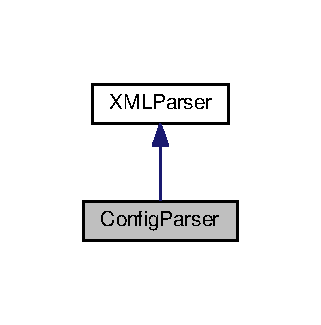
\includegraphics[width=154pt]{classConfigParser__coll__graph}
\end{center}
\end{figure}
\subsection*{Public Member Functions}
\begin{DoxyCompactItemize}
\item 
\hyperlink{classConfigParser_aa514906626a6eaa9872320410e4ab79c}{Config\+Parser} (string filename, string binary=\char`\"{}\char`\"{})
\item 
\mbox{\Hypertarget{classConfigParser_a610d3e5316be803c8f1bb7eebe32504b}\label{classConfigParser_a610d3e5316be803c8f1bb7eebe32504b}} 
virtual \hyperlink{classConfigParser_a610d3e5316be803c8f1bb7eebe32504b}{$\sim$\+Config\+Parser} ()
\begin{DoxyCompactList}\small\item\em destroy a config parser \end{DoxyCompactList}\item 
\mbox{\Hypertarget{classConfigParser_a4bc04924569bb6a49bfb8792e8421810}\label{classConfigParser_a4bc04924569bb6a49bfb8792e8421810}} 
virtual void {\bfseries parse} (\hyperlink{classconfigItemList__t}{config\+Item\+List\+\_\+t} $\ast$list, config\+A\+D\+List\+\_\+t $\ast$alist)
\end{DoxyCompactItemize}
\subsection*{Additional Inherited Members}


\subsection{Constructor \& Destructor Documentation}
\mbox{\Hypertarget{classConfigParser_aa514906626a6eaa9872320410e4ab79c}\label{classConfigParser_aa514906626a6eaa9872320410e4ab79c}} 
\index{Config\+Parser@{Config\+Parser}!Config\+Parser@{Config\+Parser}}
\index{Config\+Parser@{Config\+Parser}!Config\+Parser@{Config\+Parser}}
\subsubsection{\texorpdfstring{Config\+Parser()}{ConfigParser()}}
{\footnotesize\ttfamily Config\+Parser\+::\+Config\+Parser (\begin{DoxyParamCaption}\item[{string}]{filename,  }\item[{string}]{binary = {\ttfamily \char`\"{}\char`\"{}} }\end{DoxyParamCaption})}

construct a \hyperlink{classConfigParser}{Config\+Parser} \begin{DoxyItemize}
\item {\ttfamily filename} -\/ filename to read configuration from \item {\ttfamily binary} -\/ location of binary file, i.\+e. argv\mbox{[}0\mbox{]} \end{DoxyItemize}


The documentation for this class was generated from the following files\+:\begin{DoxyCompactItemize}
\item 
include/Config\+Parser.\+h\item 
src/Config\+Parser.\+cpp\end{DoxyCompactItemize}

\hypertarget{classCtrlComm}{}\section{Ctrl\+Comm Class Reference}
\label{classCtrlComm}\index{Ctrl\+Comm@{Ctrl\+Comm}}


{\ttfamily \#include $<$Ctrl\+Comm.\+h$>$}



Inheritance diagram for Ctrl\+Comm\+:
\nopagebreak
\begin{figure}[H]
\begin{center}
\leavevmode
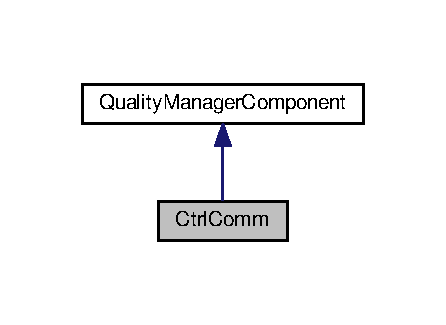
\includegraphics[width=214pt]{classCtrlComm__inherit__graph}
\end{center}
\end{figure}


Collaboration diagram for Ctrl\+Comm\+:
\nopagebreak
\begin{figure}[H]
\begin{center}
\leavevmode
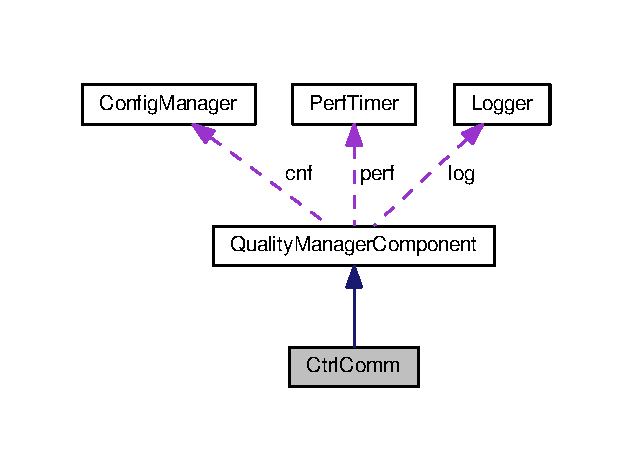
\includegraphics[width=304pt]{classCtrlComm__coll__graph}
\end{center}
\end{figure}
\subsection*{Public Member Functions}
\begin{DoxyCompactItemize}
\item 
\hyperlink{classCtrlComm_a557582fa33a0cbc4919dbfecfd1a09ac}{Ctrl\+Comm} (\hyperlink{classConfigManager}{Config\+Manager} $\ast$\hyperlink{classQualityManagerComponent_a021f9991b72d52f295b87d8a5b02046a}{cnf}, int \hyperlink{classQualityManagerComponent_add2cffa903c310563f8b999cdecd1953}{threaded}=0)
\begin{DoxyCompactList}\small\item\em construct and initialize a \hyperlink{classCtrlComm}{Ctrl\+Comm} object \end{DoxyCompactList}\item 
\mbox{\Hypertarget{classCtrlComm_a3aa5c9bb13b59ab3901010e1a20484f4}\label{classCtrlComm_a3aa5c9bb13b59ab3901010e1a20484f4}} 
\hyperlink{classCtrlComm_a3aa5c9bb13b59ab3901010e1a20484f4}{$\sim$\+Ctrl\+Comm} ()
\begin{DoxyCompactList}\small\item\em destroy a \hyperlink{classCtrlComm}{Ctrl\+Comm} object \end{DoxyCompactList}\item 
int \hyperlink{classCtrlComm_ac7b0ee75bc62a2fab69022e0ce1f507d}{access\+Check} (char $\ast$host, char $\ast$user)
\begin{DoxyCompactList}\small\item\em check if host is allowed to talk to this meter instance \end{DoxyCompactList}\item 
\mbox{\Hypertarget{classCtrlComm_a2e823214be951b2149207952c7cffab8}\label{classCtrlComm_a2e823214be951b2149207952c7cffab8}} 
int \hyperlink{classCtrlComm_a2e823214be951b2149207952c7cffab8}{log\+Access} (struct \hyperlink{structREQUEST}{R\+E\+Q\+U\+E\+ST} $\ast$req, time\+\_\+t now)
\begin{DoxyCompactList}\small\item\em log access \end{DoxyCompactList}\item 
\mbox{\Hypertarget{classCtrlComm_a7f8b660b362c7507989444f79707fcee}\label{classCtrlComm_a7f8b660b362c7507989444f79707fcee}} 
int \hyperlink{classCtrlComm_a7f8b660b362c7507989444f79707fcee}{log\+Error} (int eno, int loglevel, char $\ast$txt, char $\ast$peerhost)
\begin{DoxyCompactList}\small\item\em log error \end{DoxyCompactList}\item 
\mbox{\Hypertarget{classCtrlComm_ad61f03c20dd876772b6127a5436c2192}\label{classCtrlComm_ad61f03c20dd876772b6127a5436c2192}} 
int \hyperlink{classCtrlComm_ad61f03c20dd876772b6127a5436c2192}{handle\+F\+D\+Event} (\hyperlink{QualityManagerComponent_8h_acd67c59a21d5c694ab882c8905db0a2a}{event\+Vec\+\_\+t} $\ast$e, fd\+\_\+set $\ast$rset, fd\+\_\+set $\ast$wset, \hyperlink{structfd__sets__t}{fd\+\_\+sets\+\_\+t} $\ast$fds)
\begin{DoxyCompactList}\small\item\em handle file descriptor event \end{DoxyCompactList}\item 
\mbox{\Hypertarget{classCtrlComm_a350e593176feaefebad0ea1e68bb4e51}\label{classCtrlComm_a350e593176feaefebad0ea1e68bb4e51}} 
void \hyperlink{classCtrlComm_a350e593176feaefebad0ea1e68bb4e51}{send\+Msg} (string msg, struct \hyperlink{structREQUEST}{R\+E\+Q\+U\+E\+ST} $\ast$req, \hyperlink{structfd__sets__t}{fd\+\_\+sets\+\_\+t} $\ast$fds, int quote=1)
\begin{DoxyCompactList}\small\item\em send OK response message \end{DoxyCompactList}\item 
\mbox{\Hypertarget{classCtrlComm_a7ac459479c0772e6536da73551f3ba12}\label{classCtrlComm_a7ac459479c0772e6536da73551f3ba12}} 
void \hyperlink{classCtrlComm_a7ac459479c0772e6536da73551f3ba12}{send\+Err\+Msg} (string msg, struct \hyperlink{structREQUEST}{R\+E\+Q\+U\+E\+ST} $\ast$req, \hyperlink{structfd__sets__t}{fd\+\_\+sets\+\_\+t} $\ast$fds)
\begin{DoxyCompactList}\small\item\em send error response message \end{DoxyCompactList}\item 
\mbox{\Hypertarget{classCtrlComm_a6be57d266873bcd69afa3a98535b0b71}\label{classCtrlComm_a6be57d266873bcd69afa3a98535b0b71}} 
int \hyperlink{classCtrlComm_a6be57d266873bcd69afa3a98535b0b71}{is\+Enabled} (int feature)
\begin{DoxyCompactList}\small\item\em check whether or not a feature has been enabled on startup \end{DoxyCompactList}\item 
\mbox{\Hypertarget{classCtrlComm_ac7498c7579af7206df8a79d8b5d2f572}\label{classCtrlComm_ac7498c7579af7206df8a79d8b5d2f572}} 
int \hyperlink{classCtrlComm_ac7498c7579af7206df8a79d8b5d2f572}{get\+Timeout} ()
\begin{DoxyCompactList}\small\item\em get a timeout value ; ctrlcomm will be called in regular timeout intervals \end{DoxyCompactList}\item 
int \hyperlink{classCtrlComm_abb7de8cec0d6a04b1b722b25cb42ba5c}{process\+Cmd} (struct \hyperlink{structREQUEST}{R\+E\+Q\+U\+E\+ST} $\ast$req)
\begin{DoxyCompactList}\small\item\em process an incomming request \end{DoxyCompactList}\item 
\mbox{\Hypertarget{classCtrlComm_a3f9a7f22a18747a813268edc671b23d7}\label{classCtrlComm_a3f9a7f22a18747a813268edc671b23d7}} 
char $\ast$ \hyperlink{classCtrlComm_a3f9a7f22a18747a813268edc671b23d7}{process\+Add\+Task} (\hyperlink{structparseReq__t}{parse\+Req\+\_\+t} $\ast$preq)
\begin{DoxyCompactList}\small\item\em add a measurement task to the currently active tasks \end{DoxyCompactList}\item 
\mbox{\Hypertarget{classCtrlComm_a82207d237fd23eae2f55ff22ecd4f72c}\label{classCtrlComm_a82207d237fd23eae2f55ff22ecd4f72c}} 
char $\ast$ \hyperlink{classCtrlComm_a82207d237fd23eae2f55ff22ecd4f72c}{process\+Del\+Task} (\hyperlink{structparseReq__t}{parse\+Req\+\_\+t} $\ast$preq)
\begin{DoxyCompactList}\small\item\em delete a currently running measurement task \end{DoxyCompactList}\item 
\mbox{\Hypertarget{classCtrlComm_a62d5416d60123b5e13a613a4f7922e59}\label{classCtrlComm_a62d5416d60123b5e13a613a4f7922e59}} 
char $\ast$ \hyperlink{classCtrlComm_a62d5416d60123b5e13a613a4f7922e59}{process\+Get\+Info} (\hyperlink{structparseReq__t}{parse\+Req\+\_\+t} $\ast$preq)
\begin{DoxyCompactList}\small\item\em return meter information (tasklist,status,modlist,metercaps) \end{DoxyCompactList}\item 
\mbox{\Hypertarget{classCtrlComm_adc079d5c19f2a75eaa4a21540e3e39a7}\label{classCtrlComm_adc079d5c19f2a75eaa4a21540e3e39a7}} 
char $\ast$ \hyperlink{classCtrlComm_adc079d5c19f2a75eaa4a21540e3e39a7}{process\+Get\+Mod\+Info} (\hyperlink{structparseReq__t}{parse\+Req\+\_\+t} $\ast$preq)
\begin{DoxyCompactList}\small\item\em return process module information \end{DoxyCompactList}\item 
\mbox{\Hypertarget{classCtrlComm_a9b839913d19b1e7a57b0ff34ec4352a6}\label{classCtrlComm_a9b839913d19b1e7a57b0ff34ec4352a6}} 
void \hyperlink{classCtrlComm_a9b839913d19b1e7a57b0ff34ec4352a6}{dump} (ostream \&os)
\begin{DoxyCompactList}\small\item\em dump a \hyperlink{classCtrlComm}{Ctrl\+Comm} object \end{DoxyCompactList}\item 
\mbox{\Hypertarget{classCtrlComm_a164cf89eda1d08f441a30d9e0bcb7155}\label{classCtrlComm_a164cf89eda1d08f441a30d9e0bcb7155}} 
virtual string \hyperlink{classCtrlComm_a164cf89eda1d08f441a30d9e0bcb7155}{get\+Config\+Group} ()
\begin{DoxyCompactList}\small\item\em return name of configuration group queried by this class \end{DoxyCompactList}\end{DoxyCompactItemize}
\subsection*{Static Public Member Functions}
\begin{DoxyCompactItemize}
\item 
static int \hyperlink{classCtrlComm_a240b7eae0b93c38199b860693bfdee07}{s\+\_\+access\+\_\+check} (char $\ast$host, char $\ast$user)
\begin{DoxyCompactList}\small\item\em callback\+: check if host is allowed to talk to this meter instance \end{DoxyCompactList}\item 
\mbox{\Hypertarget{classCtrlComm_ad026f62d977a42848e04362a636ab9f1}\label{classCtrlComm_ad026f62d977a42848e04362a636ab9f1}} 
static int \hyperlink{classCtrlComm_ad026f62d977a42848e04362a636ab9f1}{s\+\_\+log\+\_\+request} (struct \hyperlink{structREQUEST}{R\+E\+Q\+U\+E\+ST} $\ast$req, time\+\_\+t now)
\begin{DoxyCompactList}\small\item\em callback method\+: log incoming request \end{DoxyCompactList}\item 
\mbox{\Hypertarget{classCtrlComm_a608fc689ad9dc6262bb1208de956e90d}\label{classCtrlComm_a608fc689ad9dc6262bb1208de956e90d}} 
static int \hyperlink{classCtrlComm_a608fc689ad9dc6262bb1208de956e90d}{s\+\_\+log\+\_\+error} (int eno, int loglevel, char $\ast$txt, char $\ast$peerhost)
\begin{DoxyCompactList}\small\item\em callback method\+: log communication error \end{DoxyCompactList}\item 
\mbox{\Hypertarget{classCtrlComm_acbb6f0eed124c17de400b895119c33dd}\label{classCtrlComm_acbb6f0eed124c17de400b895119c33dd}} 
static int {\bfseries s\+\_\+parse\+\_\+request} (struct \hyperlink{structREQUEST}{R\+E\+Q\+U\+E\+ST} $\ast$req)
\item 
static string \hyperlink{classCtrlComm_a90fc85f6b20a5fd41f70049efdb4ac7a}{xml\+Quote} (string s)
\begin{DoxyCompactList}\small\item\em convert string to new string with $<$ $>$ \& replaced by X\+ML representation \end{DoxyCompactList}\end{DoxyCompactItemize}
\subsection*{Additional Inherited Members}


\subsection{Detailed Description}
the \hyperlink{classCtrlComm}{Ctrl\+Comm} class is responsible for handling network connections to the meter. It uses H\+T\+TP as the underlying transport protocol (H\+T\+T\+PD) 

\subsection{Constructor \& Destructor Documentation}
\mbox{\Hypertarget{classCtrlComm_a557582fa33a0cbc4919dbfecfd1a09ac}\label{classCtrlComm_a557582fa33a0cbc4919dbfecfd1a09ac}} 
\index{Ctrl\+Comm@{Ctrl\+Comm}!Ctrl\+Comm@{Ctrl\+Comm}}
\index{Ctrl\+Comm@{Ctrl\+Comm}!Ctrl\+Comm@{Ctrl\+Comm}}
\subsubsection{\texorpdfstring{Ctrl\+Comm()}{CtrlComm()}}
{\footnotesize\ttfamily Ctrl\+Comm\+::\+Ctrl\+Comm (\begin{DoxyParamCaption}\item[{\hyperlink{classConfigManager}{Config\+Manager} $\ast$}]{cnf,  }\item[{int}]{threaded = {\ttfamily 0} }\end{DoxyParamCaption})}



construct and initialize a \hyperlink{classCtrlComm}{Ctrl\+Comm} object 

\begin{DoxyItemize}
\item {\ttfamily cnf} link to config manager \item {\ttfamily threaded} if 1 run as separate thread \end{DoxyItemize}


\subsection{Member Function Documentation}
\mbox{\Hypertarget{classCtrlComm_ac7b0ee75bc62a2fab69022e0ce1f507d}\label{classCtrlComm_ac7b0ee75bc62a2fab69022e0ce1f507d}} 
\index{Ctrl\+Comm@{Ctrl\+Comm}!access\+Check@{access\+Check}}
\index{access\+Check@{access\+Check}!Ctrl\+Comm@{Ctrl\+Comm}}
\subsubsection{\texorpdfstring{access\+Check()}{accessCheck()}}
{\footnotesize\ttfamily int Ctrl\+Comm\+::access\+Check (\begin{DoxyParamCaption}\item[{char $\ast$}]{host,  }\item[{char $\ast$}]{user }\end{DoxyParamCaption})}



check if host is allowed to talk to this meter instance 

\begin{DoxyReturn}{Returns}
0 if allowed, -\/1 else 
\end{DoxyReturn}
\mbox{\Hypertarget{classCtrlComm_abb7de8cec0d6a04b1b722b25cb42ba5c}\label{classCtrlComm_abb7de8cec0d6a04b1b722b25cb42ba5c}} 
\index{Ctrl\+Comm@{Ctrl\+Comm}!process\+Cmd@{process\+Cmd}}
\index{process\+Cmd@{process\+Cmd}!Ctrl\+Comm@{Ctrl\+Comm}}
\subsubsection{\texorpdfstring{process\+Cmd()}{processCmd()}}
{\footnotesize\ttfamily int Ctrl\+Comm\+::process\+Cmd (\begin{DoxyParamCaption}\item[{struct \hyperlink{structREQUEST}{R\+E\+Q\+U\+E\+ST} $\ast$}]{req }\end{DoxyParamCaption})}



process an incomming request 

parse request via sub function and queue event(s)

\begin{DoxyItemize}
\item {\ttfamily req} the incmoing request from H\+T\+T\+PD \begin{DoxyReturn}{Returns}
0 on success 
\end{DoxyReturn}
\end{DoxyItemize}
\mbox{\Hypertarget{classCtrlComm_a240b7eae0b93c38199b860693bfdee07}\label{classCtrlComm_a240b7eae0b93c38199b860693bfdee07}} 
\index{Ctrl\+Comm@{Ctrl\+Comm}!s\+\_\+access\+\_\+check@{s\+\_\+access\+\_\+check}}
\index{s\+\_\+access\+\_\+check@{s\+\_\+access\+\_\+check}!Ctrl\+Comm@{Ctrl\+Comm}}
\subsubsection{\texorpdfstring{s\+\_\+access\+\_\+check()}{s\_access\_check()}}
{\footnotesize\ttfamily static int Ctrl\+Comm\+::s\+\_\+access\+\_\+check (\begin{DoxyParamCaption}\item[{char $\ast$}]{host,  }\item[{char $\ast$}]{user }\end{DoxyParamCaption})\hspace{0.3cm}{\ttfamily [inline]}, {\ttfamily [static]}}



callback\+: check if host is allowed to talk to this meter instance 

\begin{DoxyReturn}{Returns}
0 if allowed, -\/1 else 
\end{DoxyReturn}
\mbox{\Hypertarget{classCtrlComm_a90fc85f6b20a5fd41f70049efdb4ac7a}\label{classCtrlComm_a90fc85f6b20a5fd41f70049efdb4ac7a}} 
\index{Ctrl\+Comm@{Ctrl\+Comm}!xml\+Quote@{xml\+Quote}}
\index{xml\+Quote@{xml\+Quote}!Ctrl\+Comm@{Ctrl\+Comm}}
\subsubsection{\texorpdfstring{xml\+Quote()}{xmlQuote()}}
{\footnotesize\ttfamily string Ctrl\+Comm\+::xml\+Quote (\begin{DoxyParamCaption}\item[{string}]{s }\end{DoxyParamCaption})\hspace{0.3cm}{\ttfamily [static]}}



convert string to new string with $<$ $>$ \& replaced by X\+ML representation 

\begin{DoxyItemize}
\item {\ttfamily s} -\/ the string to convert \begin{DoxyReturn}{Returns}
a new string which represents s but has $<$ $>$ \& characters replaced by \&...; 
\end{DoxyReturn}
\end{DoxyItemize}


The documentation for this class was generated from the following files\+:\begin{DoxyCompactItemize}
\item 
include/Ctrl\+Comm.\+h\item 
src/Ctrl\+Comm.\+cpp\end{DoxyCompactItemize}

\hypertarget{classCtrlCommEvent}{}\section{Ctrl\+Comm\+Event Class Reference}
\label{classCtrlCommEvent}\index{Ctrl\+Comm\+Event@{Ctrl\+Comm\+Event}}


base class for all ctrlcomm events, contains pointer to request  




{\ttfamily \#include $<$Event.\+h$>$}



Inheritance diagram for Ctrl\+Comm\+Event\+:
\nopagebreak
\begin{figure}[H]
\begin{center}
\leavevmode
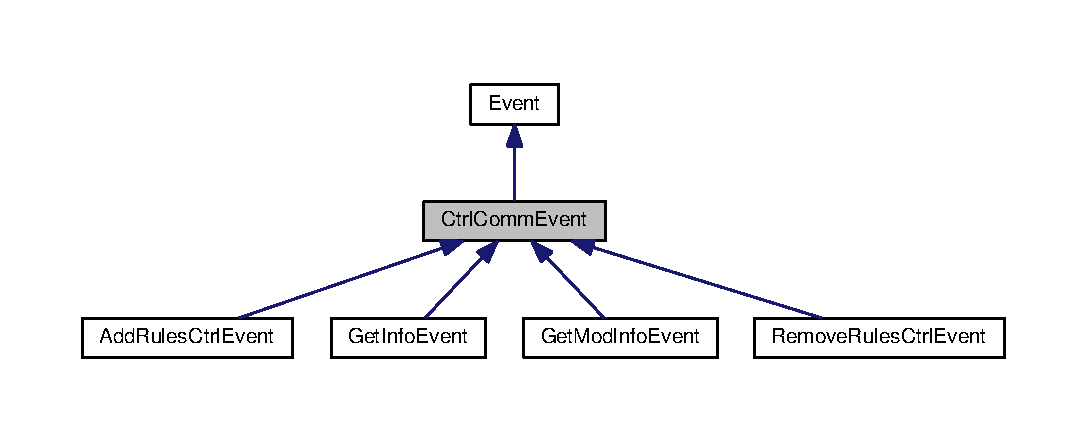
\includegraphics[width=350pt]{classCtrlCommEvent__inherit__graph}
\end{center}
\end{figure}


Collaboration diagram for Ctrl\+Comm\+Event\+:
\nopagebreak
\begin{figure}[H]
\begin{center}
\leavevmode
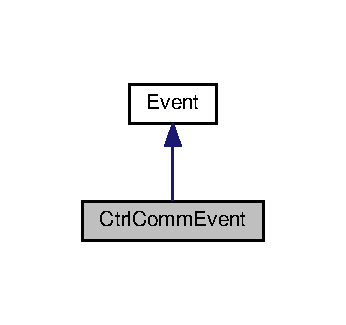
\includegraphics[width=166pt]{classCtrlCommEvent__coll__graph}
\end{center}
\end{figure}
\subsection*{Public Member Functions}
\begin{DoxyCompactItemize}
\item 
\mbox{\Hypertarget{classCtrlCommEvent_a85c1ce996cf1112a1d9f28e11af5ed66}\label{classCtrlCommEvent_a85c1ce996cf1112a1d9f28e11af5ed66}} 
\hyperlink{classCtrlCommEvent_a85c1ce996cf1112a1d9f28e11af5ed66}{Ctrl\+Comm\+Event} (\hyperlink{Event_8h_a2fb9b58e4e5f14f40af8b4a1425841f8}{event\+\_\+t} type, unsigned long ival=0, int align=0)
\begin{DoxyCompactList}\small\item\em ctrlcomm events always expire now \end{DoxyCompactList}\item 
\mbox{\Hypertarget{classCtrlCommEvent_a7fff85bd9d4c6ba4b6717aa0cfe33ef2}\label{classCtrlCommEvent_a7fff85bd9d4c6ba4b6717aa0cfe33ef2}} 
struct \hyperlink{structREQUEST}{R\+E\+Q\+U\+E\+ST} $\ast$ \hyperlink{classCtrlCommEvent_a7fff85bd9d4c6ba4b6717aa0cfe33ef2}{get\+Req} ()
\begin{DoxyCompactList}\small\item\em get request pointer \end{DoxyCompactList}\item 
\mbox{\Hypertarget{classCtrlCommEvent_a81613b45e9e386fd8407eca71e11b23f}\label{classCtrlCommEvent_a81613b45e9e386fd8407eca71e11b23f}} 
void \hyperlink{classCtrlCommEvent_a81613b45e9e386fd8407eca71e11b23f}{set\+Req} (struct \hyperlink{structREQUEST}{R\+E\+Q\+U\+E\+ST} $\ast$r)
\begin{DoxyCompactList}\small\item\em set request pointer \end{DoxyCompactList}\end{DoxyCompactItemize}


\subsection{Detailed Description}
base class for all ctrlcomm events, contains pointer to request 

The documentation for this class was generated from the following file\+:\begin{DoxyCompactItemize}
\item 
include/\hyperlink{Event_8h}{Event.\+h}\end{DoxyCompactItemize}

\hypertarget{classCtrlCommTimerEvent}{}\section{Ctrl\+Comm\+Timer\+Event Class Reference}
\label{classCtrlCommTimerEvent}\index{Ctrl\+Comm\+Timer\+Event@{Ctrl\+Comm\+Timer\+Event}}


Inheritance diagram for Ctrl\+Comm\+Timer\+Event\+:
\nopagebreak
\begin{figure}[H]
\begin{center}
\leavevmode
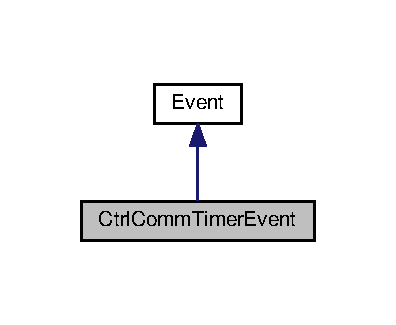
\includegraphics[width=190pt]{classCtrlCommTimerEvent__inherit__graph}
\end{center}
\end{figure}


Collaboration diagram for Ctrl\+Comm\+Timer\+Event\+:
\nopagebreak
\begin{figure}[H]
\begin{center}
\leavevmode
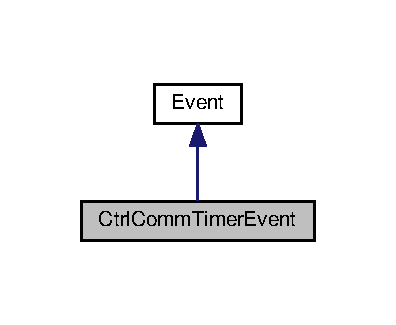
\includegraphics[width=190pt]{classCtrlCommTimerEvent__coll__graph}
\end{center}
\end{figure}
\subsection*{Public Member Functions}
\begin{DoxyCompactItemize}
\item 
\mbox{\Hypertarget{classCtrlCommTimerEvent_a75281b9d41f9f484711fd4d5fa09fe16}\label{classCtrlCommTimerEvent_a75281b9d41f9f484711fd4d5fa09fe16}} 
{\bfseries Ctrl\+Comm\+Timer\+Event} (time\+\_\+t offs\+\_\+sec, unsigned long ival=0, int align=0)
\end{DoxyCompactItemize}


The documentation for this class was generated from the following file\+:\begin{DoxyCompactItemize}
\item 
include/\hyperlink{Event_8h}{Event.\+h}\end{DoxyCompactItemize}

\hypertarget{classError}{}\section{Error Class Reference}
\label{classError}\index{Error@{Error}}


generic error exception  




{\ttfamily \#include $<$Error.\+h$>$}

\subsection*{Public Member Functions}
\begin{DoxyCompactItemize}
\item 
\hyperlink{classError_aca339d00ad8481fb4c184f0ece42698b}{Error} ()
\begin{DoxyCompactList}\small\item\em $<$ create unnamed error exception \end{DoxyCompactList}\item 
\mbox{\Hypertarget{classError_a33c9f1966a27831eb49342ae02107fe5}\label{classError_a33c9f1966a27831eb49342ae02107fe5}} 
\hyperlink{classError_a33c9f1966a27831eb49342ae02107fe5}{Error} (const std\+::string new\+\_\+error=\char`\"{}\char`\"{})
\begin{DoxyCompactList}\small\item\em create named error exception \end{DoxyCompactList}\item 
\mbox{\Hypertarget{classError_ae83a1b2e22001c74cb433c9db4b06c59}\label{classError_ae83a1b2e22001c74cb433c9db4b06c59}} 
\hyperlink{classError_ae83a1b2e22001c74cb433c9db4b06c59}{Error} (const int err\+\_\+no=0, const std\+::string err\+\_\+str=\char`\"{}\char`\"{})
\begin{DoxyCompactList}\small\item\em printf-\/style constructor \end{DoxyCompactList}\item 
\mbox{\Hypertarget{classError_a3c4ebf23ad22025f4c3144318a4ccd3b}\label{classError_a3c4ebf23ad22025f4c3144318a4ccd3b}} 
\hyperlink{classError_a3c4ebf23ad22025f4c3144318a4ccd3b}{Error} (const int err\+\_\+no, const char $\ast$fmt,...)
\begin{DoxyCompactList}\small\item\em printf-\/style constructor \end{DoxyCompactList}\item 
\mbox{\Hypertarget{classError_a04b610b88a09921231dbfd10f41b3d11}\label{classError_a04b610b88a09921231dbfd10f41b3d11}} 
\hyperlink{classError_a04b610b88a09921231dbfd10f41b3d11}{Error} (const char $\ast$fmt,...)
\begin{DoxyCompactList}\small\item\em get error msg from exception \end{DoxyCompactList}\item 
\mbox{\Hypertarget{classError_aa2aec02f62fb7e8325c5bb793da64a90}\label{classError_aa2aec02f62fb7e8325c5bb793da64a90}} 
std\+::string {\bfseries get\+Error} ()
\item 
\mbox{\Hypertarget{classError_a74ba8bd7fd5b5361be11daee8b5c6b1c}\label{classError_a74ba8bd7fd5b5361be11daee8b5c6b1c}} 
int \hyperlink{classError_a74ba8bd7fd5b5361be11daee8b5c6b1c}{get\+Error\+No} ()
\begin{DoxyCompactList}\small\item\em get error number \end{DoxyCompactList}\item 
\mbox{\Hypertarget{classError_a1a2e5f78dedac07786fe06969672eea7}\label{classError_a1a2e5f78dedac07786fe06969672eea7}} 
void {\bfseries dump} (std\+::ostream \&os)
\end{DoxyCompactItemize}
\subsection*{Protected Attributes}
\begin{DoxyCompactItemize}
\item 
int \hyperlink{classError_aca10c20ddc3769ff18c87d98052bbc3e}{error\+No}
\begin{DoxyCompactList}\small\item\em error number \end{DoxyCompactList}\item 
\mbox{\Hypertarget{classError_a7ca1958fd4898587d70b88c0c0dc0695}\label{classError_a7ca1958fd4898587d70b88c0c0dc0695}} 
std\+::string {\bfseries error}
\end{DoxyCompactItemize}


\subsection{Detailed Description}
generic error exception 

\hyperlink{classError}{Error} represents an exception that can be thrown. It includes a string that can be used to further specify the error encountered. Optionally it also includes a number. 

\subsection{Constructor \& Destructor Documentation}
\mbox{\Hypertarget{classError_aca339d00ad8481fb4c184f0ece42698b}\label{classError_aca339d00ad8481fb4c184f0ece42698b}} 
\index{Error@{Error}!Error@{Error}}
\index{Error@{Error}!Error@{Error}}
\subsubsection{\texorpdfstring{Error()}{Error()}}
{\footnotesize\ttfamily Error\+::\+Error (\begin{DoxyParamCaption}{ }\end{DoxyParamCaption})\hspace{0.3cm}{\ttfamily [inline]}}



$<$ create unnamed error exception 

create named error exception 

\subsection{Member Data Documentation}
\mbox{\Hypertarget{classError_aca10c20ddc3769ff18c87d98052bbc3e}\label{classError_aca10c20ddc3769ff18c87d98052bbc3e}} 
\index{Error@{Error}!error\+No@{error\+No}}
\index{error\+No@{error\+No}!Error@{Error}}
\subsubsection{\texorpdfstring{error\+No}{errorNo}}
{\footnotesize\ttfamily int Error\+::error\+No\hspace{0.3cm}{\ttfamily [protected]}}



error number 

error string 

The documentation for this class was generated from the following files\+:\begin{DoxyCompactItemize}
\item 
include/\hyperlink{Error_8h}{Error.\+h}\item 
src/Error.\+cpp\end{DoxyCompactItemize}

\hypertarget{classEvent}{}\section{Event Class Reference}
\label{classEvent}\index{Event@{Event}}


basic event element that is the base class of all other events that can be stored in the event queue of \hyperlink{classEventScheduler}{Event\+Scheduler}  




{\ttfamily \#include $<$Event.\+h$>$}



Inheritance diagram for Event\+:
\nopagebreak
\begin{figure}[H]
\begin{center}
\leavevmode
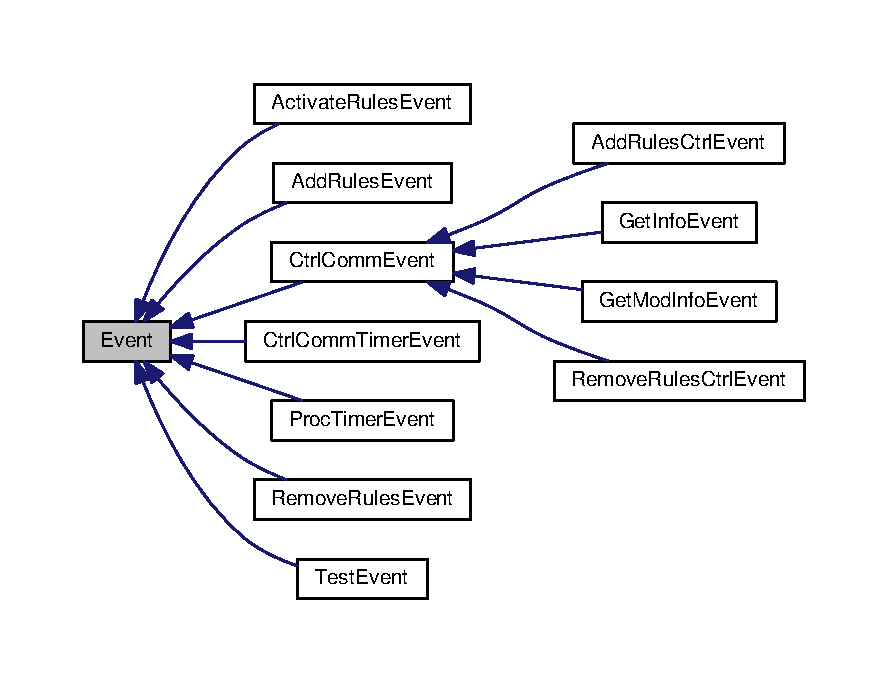
\includegraphics[width=350pt]{classEvent__inherit__graph}
\end{center}
\end{figure}
\subsection*{Public Member Functions}
\begin{DoxyCompactItemize}
\item 
\hyperlink{classEvent_acd3f54caeb58e6375e51a044c0ee2616}{Event} (\hyperlink{Event_8h_a2fb9b58e4e5f14f40af8b4a1425841f8}{event\+\_\+t} type, struct timeval time, unsigned long ival=0, int align=0)
\begin{DoxyCompactList}\small\item\em create an event at an absolute time \end{DoxyCompactList}\item 
\hyperlink{classEvent_a0b28a5ecf2af747c56b9cdcd2e26642b}{Event} (\hyperlink{Event_8h_a2fb9b58e4e5f14f40af8b4a1425841f8}{event\+\_\+t} type, time\+\_\+t offs\+\_\+sec, time\+\_\+t offs\+\_\+usec=0, unsigned long ival=0, int align=0)
\begin{DoxyCompactList}\small\item\em create an event relative to current time \end{DoxyCompactList}\item 
\hyperlink{classEvent_a9fa90b8cff91b5d58a7fbd690e1bcfaa}{Event} (\hyperlink{Event_8h_a2fb9b58e4e5f14f40af8b4a1425841f8}{event\+\_\+t} type, unsigned long ival=0, int align=0)
\begin{DoxyCompactList}\small\item\em create an event at the current time (now) \end{DoxyCompactList}\item 
\mbox{\Hypertarget{classEvent_a7682b6c4066b0733a61bae0a4c7110da}\label{classEvent_a7682b6c4066b0733a61bae0a4c7110da}} 
\hyperlink{Event_8h_a2fb9b58e4e5f14f40af8b4a1425841f8}{event\+\_\+t} \hyperlink{classEvent_a7682b6c4066b0733a61bae0a4c7110da}{get\+Type} ()
\begin{DoxyCompactList}\small\item\em get event type \end{DoxyCompactList}\item 
\mbox{\Hypertarget{classEvent_a197eb389db5c5e98fd6f4fa762f1f23e}\label{classEvent_a197eb389db5c5e98fd6f4fa762f1f23e}} 
int {\bfseries is\+Type} (\hyperlink{Event_8h_a2fb9b58e4e5f14f40af8b4a1425841f8}{event\+\_\+t} atype)
\item 
\mbox{\Hypertarget{classEvent_acee8c5f11e9706148029e7cc78db3f7f}\label{classEvent_acee8c5f11e9706148029e7cc78db3f7f}} 
struct timeval \hyperlink{classEvent_acee8c5f11e9706148029e7cc78db3f7f}{get\+Time} ()
\begin{DoxyCompactList}\small\item\em get expiry time \end{DoxyCompactList}\item 
\mbox{\Hypertarget{classEvent_ab3c5d8d6c110eb033389638746a02ddd}\label{classEvent_ab3c5d8d6c110eb033389638746a02ddd}} 
unsigned long \hyperlink{classEvent_ab3c5d8d6c110eb033389638746a02ddd}{get\+Ival} ()
\begin{DoxyCompactList}\small\item\em get interval \end{DoxyCompactList}\item 
\mbox{\Hypertarget{classEvent_aab363fcc2a278a4c58e2d0d4bd61b4c4}\label{classEvent_aab363fcc2a278a4c58e2d0d4bd61b4c4}} 
void \hyperlink{classEvent_aab363fcc2a278a4c58e2d0d4bd61b4c4}{set\+Interval} (unsigned long ival)
\begin{DoxyCompactList}\small\item\em set interval \end{DoxyCompactList}\item 
\mbox{\Hypertarget{classEvent_aa539db91725efa367bc51bd20c6f6527}\label{classEvent_aa539db91725efa367bc51bd20c6f6527}} 
void \hyperlink{classEvent_aa539db91725efa367bc51bd20c6f6527}{set\+Time} (struct timeval new\+Time)
\begin{DoxyCompactList}\small\item\em set expiry time \end{DoxyCompactList}\item 
\mbox{\Hypertarget{classEvent_a1b15a8aed3a94f247adb883ecebc5cbd}\label{classEvent_a1b15a8aed3a94f247adb883ecebc5cbd}} 
void \hyperlink{classEvent_a1b15a8aed3a94f247adb883ecebc5cbd}{set\+Time} (time\+\_\+t new\+Time\+Sec)
\begin{DoxyCompactList}\small\item\em set expiry time (full sec) \end{DoxyCompactList}\item 
\mbox{\Hypertarget{classEvent_ac401a0dcd7f2dd526015285ac827f61b}\label{classEvent_ac401a0dcd7f2dd526015285ac827f61b}} 
void \hyperlink{classEvent_ac401a0dcd7f2dd526015285ac827f61b}{advance} ()
\begin{DoxyCompactList}\small\item\em get next expiry time (recurrent events) \end{DoxyCompactList}\item 
\mbox{\Hypertarget{classEvent_a1a0e50aa2d50ba782fb78c369c40762f}\label{classEvent_a1a0e50aa2d50ba782fb78c369c40762f}} 
virtual void {\bfseries dump} (ostream \&os)
\item 
\mbox{\Hypertarget{classEvent_a1784b321b36147c83c469435629db298}\label{classEvent_a1784b321b36147c83c469435629db298}} 
virtual int \hyperlink{classEvent_a1784b321b36147c83c469435629db298}{delete\+Rule} (int uid)
\begin{DoxyCompactList}\small\item\em delete rules stored in this event \end{DoxyCompactList}\end{DoxyCompactItemize}


\subsection{Detailed Description}
basic event element that is the base class of all other events that can be stored in the event queue of \hyperlink{classEventScheduler}{Event\+Scheduler} 

\subsection{Constructor \& Destructor Documentation}
\mbox{\Hypertarget{classEvent_acd3f54caeb58e6375e51a044c0ee2616}\label{classEvent_acd3f54caeb58e6375e51a044c0ee2616}} 
\index{Event@{Event}!Event@{Event}}
\index{Event@{Event}!Event@{Event}}
\subsubsection{\texorpdfstring{Event()}{Event()}\hspace{0.1cm}{\footnotesize\ttfamily [1/3]}}
{\footnotesize\ttfamily Event\+::\+Event (\begin{DoxyParamCaption}\item[{\hyperlink{Event_8h_a2fb9b58e4e5f14f40af8b4a1425841f8}{event\+\_\+t}}]{type,  }\item[{struct timeval}]{time,  }\item[{unsigned long}]{ival = {\ttfamily 0},  }\item[{int}]{align = {\ttfamily 0} }\end{DoxyParamCaption})}



create an event at an absolute time 

\begin{DoxyItemize}
\item {\ttfamily type} type of the event \item {\ttfamily time} absolute timestamp when the event is due \item {\ttfamily ival} interval (in ms) if the event is recurrent \item {\ttfamily align} align the event on the next ival \end{DoxyItemize}
\mbox{\Hypertarget{classEvent_a0b28a5ecf2af747c56b9cdcd2e26642b}\label{classEvent_a0b28a5ecf2af747c56b9cdcd2e26642b}} 
\index{Event@{Event}!Event@{Event}}
\index{Event@{Event}!Event@{Event}}
\subsubsection{\texorpdfstring{Event()}{Event()}\hspace{0.1cm}{\footnotesize\ttfamily [2/3]}}
{\footnotesize\ttfamily Event\+::\+Event (\begin{DoxyParamCaption}\item[{\hyperlink{Event_8h_a2fb9b58e4e5f14f40af8b4a1425841f8}{event\+\_\+t}}]{type,  }\item[{time\+\_\+t}]{offs\+\_\+sec,  }\item[{time\+\_\+t}]{offs\+\_\+usec = {\ttfamily 0},  }\item[{unsigned long}]{ival = {\ttfamily 0},  }\item[{int}]{align = {\ttfamily 0} }\end{DoxyParamCaption})}



create an event relative to current time 

\begin{DoxyItemize}
\item {\ttfamily type} type of the event \item {\ttfamily offs\+\_\+sec} sec offset from now when the event is due \item {\ttfamily offs\+\_\+used} usec offset from now when the event is due \item {\ttfamily ival} interval (in ms) if the event is recurrent \item {\ttfamily align} align the event on the next ival \end{DoxyItemize}
\mbox{\Hypertarget{classEvent_a9fa90b8cff91b5d58a7fbd690e1bcfaa}\label{classEvent_a9fa90b8cff91b5d58a7fbd690e1bcfaa}} 
\index{Event@{Event}!Event@{Event}}
\index{Event@{Event}!Event@{Event}}
\subsubsection{\texorpdfstring{Event()}{Event()}\hspace{0.1cm}{\footnotesize\ttfamily [3/3]}}
{\footnotesize\ttfamily Event\+::\+Event (\begin{DoxyParamCaption}\item[{\hyperlink{Event_8h_a2fb9b58e4e5f14f40af8b4a1425841f8}{event\+\_\+t}}]{type,  }\item[{unsigned long}]{ival = {\ttfamily 0},  }\item[{int}]{align = {\ttfamily 0} }\end{DoxyParamCaption})}



create an event at the current time (now) 

\begin{DoxyItemize}
\item {\ttfamily type} type of the event \item {\ttfamily ival} interval (in ms) if the event is recurrent \item {\ttfamily align} align the event on the next ival \end{DoxyItemize}


The documentation for this class was generated from the following files\+:\begin{DoxyCompactItemize}
\item 
include/\hyperlink{Event_8h}{Event.\+h}\item 
src/\hyperlink{Event_8cpp}{Event.\+cpp}\end{DoxyCompactItemize}

\hypertarget{classEventScheduler}{}\section{Event\+Scheduler Class Reference}
\label{classEventScheduler}\index{Event\+Scheduler@{Event\+Scheduler}}


schedule timed events and execute the corresponding function at the correct time  




{\ttfamily \#include $<$Event\+Scheduler.\+h$>$}

\subsection*{Public Member Functions}
\begin{DoxyCompactItemize}
\item 
\mbox{\Hypertarget{classEventScheduler_a5d0af0bdbbb5948ab06075ef12fc8aa0}\label{classEventScheduler_a5d0af0bdbbb5948ab06075ef12fc8aa0}} 
\hyperlink{classEventScheduler_a5d0af0bdbbb5948ab06075ef12fc8aa0}{Event\+Scheduler} ()
\begin{DoxyCompactList}\small\item\em construct and initialize an \hyperlink{classEventScheduler}{Event\+Scheduler} object \end{DoxyCompactList}\item 
\mbox{\Hypertarget{classEventScheduler_a30d88ffd8a9c7956947ccf0dc58e20ac}\label{classEventScheduler_a30d88ffd8a9c7956947ccf0dc58e20ac}} 
\hyperlink{classEventScheduler_a30d88ffd8a9c7956947ccf0dc58e20ac}{$\sim$\+Event\+Scheduler} ()
\begin{DoxyCompactList}\small\item\em destroy an \hyperlink{classEventScheduler}{Event\+Scheduler} object \end{DoxyCompactList}\item 
void \hyperlink{classEventScheduler_aa0ece0b48922f1712e0d1057841e1c0f}{add\+Event} (\hyperlink{classEvent}{Event} $\ast$ev)
\begin{DoxyCompactList}\small\item\em add an \hyperlink{classEvent}{Event} to the event queue \end{DoxyCompactList}\item 
void \hyperlink{classEventScheduler_a2f6d1f0ef1f8ef3b073f99ae9ecc1f35}{del\+Rule\+Events} (int uid)
\begin{DoxyCompactList}\small\item\em delete all events for a given rule \end{DoxyCompactList}\item 
\mbox{\Hypertarget{classEventScheduler_a8c920197e971dc108bfa5847d68696d0}\label{classEventScheduler_a8c920197e971dc108bfa5847d68696d0}} 
\hyperlink{classEvent}{Event} $\ast$ {\bfseries get\+Next\+Event} ()
\item 
\mbox{\Hypertarget{classEventScheduler_a44080cd7623b245afdabb2ddfcf7c6a3}\label{classEventScheduler_a44080cd7623b245afdabb2ddfcf7c6a3}} 
void \hyperlink{classEventScheduler_a44080cd7623b245afdabb2ddfcf7c6a3}{resched\+Next\+Event} (\hyperlink{classEvent}{Event} $\ast$ev)
\begin{DoxyCompactList}\small\item\em requeus (if recurring) the event ev advancing its expiry time \end{DoxyCompactList}\item 
\mbox{\Hypertarget{classEventScheduler_ad77fed3420f8ef0c07a2dbb8e7ccfd3b}\label{classEventScheduler_ad77fed3420f8ef0c07a2dbb8e7ccfd3b}} 
struct timeval \hyperlink{classEventScheduler_ad77fed3420f8ef0c07a2dbb8e7ccfd3b}{get\+Next\+Event\+Time} ()
\begin{DoxyCompactList}\small\item\em return the time of the next event due \end{DoxyCompactList}\item 
\mbox{\Hypertarget{classEventScheduler_ac479416f6764531401c2ca21b774ea52}\label{classEventScheduler_ac479416f6764531401c2ca21b774ea52}} 
void \hyperlink{classEventScheduler_ac479416f6764531401c2ca21b774ea52}{dump} (ostream \&os)
\begin{DoxyCompactList}\small\item\em dump an \hyperlink{classEventScheduler}{Event\+Scheduler} object \end{DoxyCompactList}\end{DoxyCompactItemize}


\subsection{Detailed Description}
schedule timed events and execute the corresponding function at the correct time 

The \hyperlink{classEventScheduler}{Event\+Scheduler}\textquotesingle{}s task is to schedule and execute timed events in the meter system such as timed addition/removal of tasks (rules). A number of different events that are derived from the basic event class can be put into the Event\+Schedulers event queue. 

\subsection{Member Function Documentation}
\mbox{\Hypertarget{classEventScheduler_aa0ece0b48922f1712e0d1057841e1c0f}\label{classEventScheduler_aa0ece0b48922f1712e0d1057841e1c0f}} 
\index{Event\+Scheduler@{Event\+Scheduler}!add\+Event@{add\+Event}}
\index{add\+Event@{add\+Event}!Event\+Scheduler@{Event\+Scheduler}}
\subsubsection{\texorpdfstring{add\+Event()}{addEvent()}}
{\footnotesize\ttfamily void Event\+Scheduler\+::add\+Event (\begin{DoxyParamCaption}\item[{\hyperlink{classEvent}{Event} $\ast$}]{ev }\end{DoxyParamCaption})}



add an \hyperlink{classEvent}{Event} to the event queue 

\begin{DoxyItemize}
\item {\ttfamily ev} -\/ an event (or an object derived from \hyperlink{classEvent}{Event}) that is schdeuled for a particular time (possibly repeatedly at a given interval) \end{DoxyItemize}
\mbox{\Hypertarget{classEventScheduler_a2f6d1f0ef1f8ef3b073f99ae9ecc1f35}\label{classEventScheduler_a2f6d1f0ef1f8ef3b073f99ae9ecc1f35}} 
\index{Event\+Scheduler@{Event\+Scheduler}!del\+Rule\+Events@{del\+Rule\+Events}}
\index{del\+Rule\+Events@{del\+Rule\+Events}!Event\+Scheduler@{Event\+Scheduler}}
\subsubsection{\texorpdfstring{del\+Rule\+Events()}{delRuleEvents()}}
{\footnotesize\ttfamily void Event\+Scheduler\+::del\+Rule\+Events (\begin{DoxyParamCaption}\item[{int}]{uid }\end{DoxyParamCaption})}



delete all events for a given rule 

delete all Events related to the specified rule from the list of events

\begin{DoxyItemize}
\item {\ttfamily uid} -\/ the unique identification number of the rule\end{DoxyItemize}
deleting is costly but it should occur much less than exporting data or flow timeouts assuming the lifetimes of rules are reasonably large 

The documentation for this class was generated from the following files\+:\begin{DoxyCompactItemize}
\item 
include/\hyperlink{EventScheduler_8h}{Event\+Scheduler.\+h}\item 
src/Event\+Scheduler.\+cpp\end{DoxyCompactItemize}

\hypertarget{structfd__sets__t}{}\section{fd\+\_\+sets\+\_\+t Struct Reference}
\label{structfd__sets__t}\index{fd\+\_\+sets\+\_\+t@{fd\+\_\+sets\+\_\+t}}
\subsection*{Public Attributes}
\begin{DoxyCompactItemize}
\item 
\mbox{\Hypertarget{structfd__sets__t_a7ff7ae153d4d1029835242522591c255}\label{structfd__sets__t_a7ff7ae153d4d1029835242522591c255}} 
int {\bfseries max}
\item 
\mbox{\Hypertarget{structfd__sets__t_a522141a7a01c484a7a95d18b4913f093}\label{structfd__sets__t_a522141a7a01c484a7a95d18b4913f093}} 
fd\+\_\+set {\bfseries rset}
\item 
\mbox{\Hypertarget{structfd__sets__t_af96615f7cd29f97271f5f635d2f07e9c}\label{structfd__sets__t_af96615f7cd29f97271f5f635d2f07e9c}} 
fd\+\_\+set {\bfseries wset}
\end{DoxyCompactItemize}


The documentation for this struct was generated from the following file\+:\begin{DoxyCompactItemize}
\item 
lib/httpd/\hyperlink{httpd_8h}{httpd.\+h}\end{DoxyCompactItemize}

\hypertarget{structfd__t}{}\section{fd\+\_\+t Struct Reference}
\label{structfd__t}\index{fd\+\_\+t@{fd\+\_\+t}}
\subsection*{Public Attributes}
\begin{DoxyCompactItemize}
\item 
\mbox{\Hypertarget{structfd__t_a202e5b3abfffce509eeae0035a40bb0e}\label{structfd__t_a202e5b3abfffce509eeae0035a40bb0e}} 
int {\bfseries fd}
\item 
\mbox{\Hypertarget{structfd__t_ac051505ddc0ed97d122a4cf23e2f5eb9}\label{structfd__t_ac051505ddc0ed97d122a4cf23e2f5eb9}} 
int {\bfseries mode}
\end{DoxyCompactItemize}


The documentation for this struct was generated from the following file\+:\begin{DoxyCompactItemize}
\item 
lib/httpd/\hyperlink{httpd_8h}{httpd.\+h}\end{DoxyCompactItemize}

\hypertarget{structfilter__t}{}\section{filter\+\_\+t Struct Reference}
\label{structfilter__t}\index{filter\+\_\+t@{filter\+\_\+t}}


definition of a filter  




{\ttfamily \#include $<$Proc\+Module\+Interface.\+h$>$}



Collaboration diagram for filter\+\_\+t\+:
\nopagebreak
\begin{figure}[H]
\begin{center}
\leavevmode
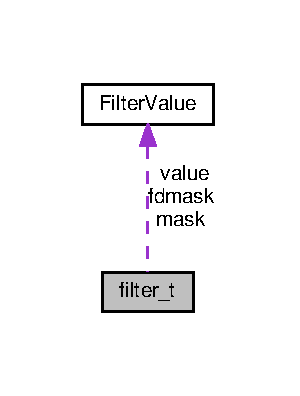
\includegraphics[width=144pt]{structfilter__t__coll__graph}
\end{center}
\end{figure}
\subsection*{Public Attributes}
\begin{DoxyCompactItemize}
\item 
\mbox{\Hypertarget{structfilter__t_a7d320a6a351d09f1d5720edfff374361}\label{structfilter__t_a7d320a6a351d09f1d5720edfff374361}} 
string {\bfseries name}
\item 
\mbox{\Hypertarget{structfilter__t_ad52f66e4ab62c0043d4d7c38256386f2}\label{structfilter__t_ad52f66e4ab62c0043d4d7c38256386f2}} 
string {\bfseries rname}
\item 
\mbox{\Hypertarget{structfilter__t_a1a4367c07a7777feada9689d5086d4af}\label{structfilter__t_a1a4367c07a7777feada9689d5086d4af}} 
string {\bfseries type}
\item 
\mbox{\Hypertarget{structfilter__t_a59ee5af195722a38a7e349a683964815}\label{structfilter__t_a59ee5af195722a38a7e349a683964815}} 
\hyperlink{ProcModuleInterface_8h_ad660177f0843f6899357d549c92d206c}{filter\+Type\+\_\+t} {\bfseries mtype}
\item 
\mbox{\Hypertarget{structfilter__t_a46615dc949298c13405fc055d6d2836b}\label{structfilter__t_a46615dc949298c13405fc055d6d2836b}} 
refer\+\_\+t {\bfseries refer}
\item 
\mbox{\Hypertarget{structfilter__t_a3ff8b57dcc7fabd31253c8db83869a10}\label{structfilter__t_a3ff8b57dcc7fabd31253c8db83869a10}} 
refer\+\_\+t {\bfseries rrefer}
\item 
\mbox{\Hypertarget{structfilter__t_a5cc076209cea0cc04bd787c4dfea7403}\label{structfilter__t_a5cc076209cea0cc04bd787c4dfea7403}} 
unsigned short {\bfseries offs}
\item 
\mbox{\Hypertarget{structfilter__t_a116abdf5ab9853b15745c63555f9843d}\label{structfilter__t_a116abdf5ab9853b15745c63555f9843d}} 
unsigned short {\bfseries roffs}
\item 
\mbox{\Hypertarget{structfilter__t_a1d8299db10770218540bf68b5a99dc61}\label{structfilter__t_a1d8299db10770218540bf68b5a99dc61}} 
unsigned short {\bfseries len}
\item 
\mbox{\Hypertarget{structfilter__t_a31622b173ff184f93fb72ca5330929eb}\label{structfilter__t_a31622b173ff184f93fb72ca5330929eb}} 
unsigned short \hyperlink{structfilter__t_a31622b173ff184f93fb72ca5330929eb}{cnt}
\begin{DoxyCompactList}\small\item\em number of values \end{DoxyCompactList}\item 
\mbox{\Hypertarget{structfilter__t_ac228e14b328ecffc695a47dbdc4e7c72}\label{structfilter__t_ac228e14b328ecffc695a47dbdc4e7c72}} 
\hyperlink{classFilterValue}{Filter\+Value} \hyperlink{structfilter__t_ac228e14b328ecffc695a47dbdc4e7c72}{fdmask}
\begin{DoxyCompactList}\small\item\em mask from filter definition \end{DoxyCompactList}\item 
\mbox{\Hypertarget{structfilter__t_a42fe28ebb94afd681d5e495916e4a71d}\label{structfilter__t_a42fe28ebb94afd681d5e495916e4a71d}} 
unsigned char \hyperlink{structfilter__t_a42fe28ebb94afd681d5e495916e4a71d}{fdshift}
\begin{DoxyCompactList}\small\item\em position of lowest set bit in fdmask (only set when len == 1) \end{DoxyCompactList}\item 
\mbox{\Hypertarget{structfilter__t_a8b06d443a853adc1606cfae366ee9e80}\label{structfilter__t_a8b06d443a853adc1606cfae366ee9e80}} 
\hyperlink{classFilterValue}{Filter\+Value} \hyperlink{structfilter__t_a8b06d443a853adc1606cfae366ee9e80}{mask}
\begin{DoxyCompactList}\small\item\em mask for the filter value \end{DoxyCompactList}\item 
\hyperlink{classFilterValue}{Filter\+Value} \hyperlink{structfilter__t_a360ab1655062e64bbebdefd3acb749b6}{value} \mbox{[}M\+A\+X\+\_\+\+F\+I\+L\+T\+E\+R\+\_\+\+S\+E\+T\+\_\+\+S\+I\+ZE\mbox{]}
\end{DoxyCompactItemize}


\subsection{Detailed Description}
definition of a filter 

\subsection{Member Data Documentation}
\mbox{\Hypertarget{structfilter__t_a360ab1655062e64bbebdefd3acb749b6}\label{structfilter__t_a360ab1655062e64bbebdefd3acb749b6}} 
\index{filter\+\_\+t@{filter\+\_\+t}!value@{value}}
\index{value@{value}!filter\+\_\+t@{filter\+\_\+t}}
\subsubsection{\texorpdfstring{value}{value}}
{\footnotesize\ttfamily \hyperlink{classFilterValue}{Filter\+Value} filter\+\_\+t\+::value\mbox{[}M\+A\+X\+\_\+\+F\+I\+L\+T\+E\+R\+\_\+\+S\+E\+T\+\_\+\+S\+I\+ZE\mbox{]}}

value definition\+: E\+X\+A\+CT -\/$>$ value\mbox{[}0\mbox{]} R\+A\+N\+GE -\/$>$ min in value\mbox{[}0\mbox{]}, max in value\mbox{[}1\mbox{]} S\+ET -\/$>$ value\mbox{[}0-\/n\mbox{]} where value.\+len$>$0 W\+I\+LD -\/$>$ no value 

The documentation for this struct was generated from the following file\+:\begin{DoxyCompactItemize}
\item 
include/\hyperlink{ProcModuleInterface_8h}{Proc\+Module\+Interface.\+h}\end{DoxyCompactItemize}

\hypertarget{structfilterDefItem__t}{}\section{filter\+Def\+Item\+\_\+t Struct Reference}
\label{structfilterDefItem__t}\index{filter\+Def\+Item\+\_\+t@{filter\+Def\+Item\+\_\+t}}


filter definition  




{\ttfamily \#include $<$Filter\+Def\+Parser.\+h$>$}



Collaboration diagram for filter\+Def\+Item\+\_\+t\+:
\nopagebreak
\begin{figure}[H]
\begin{center}
\leavevmode
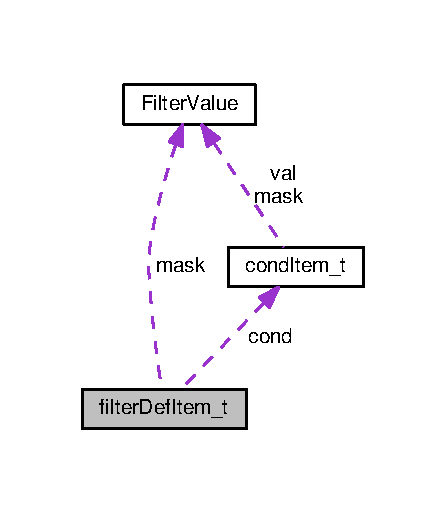
\includegraphics[width=214pt]{structfilterDefItem__t__coll__graph}
\end{center}
\end{figure}
\subsection*{Public Attributes}
\begin{DoxyCompactItemize}
\item 
\mbox{\Hypertarget{structfilterDefItem__t_a53b83e74cf05841d193eba0458587300}\label{structfilterDefItem__t_a53b83e74cf05841d193eba0458587300}} 
string {\bfseries name}
\item 
\mbox{\Hypertarget{structfilterDefItem__t_a7df261baeb794a4e3af5d58292181e71}\label{structfilterDefItem__t_a7df261baeb794a4e3af5d58292181e71}} 
string {\bfseries rname}
\item 
\mbox{\Hypertarget{structfilterDefItem__t_a52e57501e1440c062ae27b2a5d829113}\label{structfilterDefItem__t_a52e57501e1440c062ae27b2a5d829113}} 
string {\bfseries type}
\item 
\mbox{\Hypertarget{structfilterDefItem__t_aa9af5e33efd8edf71e355f52c2327511}\label{structfilterDefItem__t_aa9af5e33efd8edf71e355f52c2327511}} 
refer\+\_\+t {\bfseries refer}
\item 
\mbox{\Hypertarget{structfilterDefItem__t_a2ca1d76d1b4444ce7ea5ea8edb5ec241}\label{structfilterDefItem__t_a2ca1d76d1b4444ce7ea5ea8edb5ec241}} 
\hyperlink{structcondItem__t}{cond\+Item\+\_\+t} {\bfseries cond}
\item 
\mbox{\Hypertarget{structfilterDefItem__t_a4b80c99e2ab8f379d9d8201fd1ca2bd0}\label{structfilterDefItem__t_a4b80c99e2ab8f379d9d8201fd1ca2bd0}} 
unsigned short {\bfseries offs}
\item 
\mbox{\Hypertarget{structfilterDefItem__t_a628542cd24e504d019bb2239647db338}\label{structfilterDefItem__t_a628542cd24e504d019bb2239647db338}} 
unsigned short {\bfseries len}
\item 
\mbox{\Hypertarget{structfilterDefItem__t_a1d9bb34646ad79c48e8d9f4a515cb16f}\label{structfilterDefItem__t_a1d9bb34646ad79c48e8d9f4a515cb16f}} 
\hyperlink{classFilterValue}{Filter\+Value} {\bfseries mask}
\item 
\mbox{\Hypertarget{structfilterDefItem__t_abd3540baed1e4269a6d4a5367ce05735}\label{structfilterDefItem__t_abd3540baed1e4269a6d4a5367ce05735}} 
unsigned char \hyperlink{structfilterDefItem__t_abd3540baed1e4269a6d4a5367ce05735}{shift}
\begin{DoxyCompactList}\small\item\em position of lowest set bit in mask (only computed for len == 1) \end{DoxyCompactList}\end{DoxyCompactItemize}


\subsection{Detailed Description}
filter definition 

The documentation for this struct was generated from the following file\+:\begin{DoxyCompactItemize}
\item 
include/Filter\+Def\+Parser.\+h\end{DoxyCompactItemize}

\hypertarget{classFilterDefParser}{}\section{Filter\+Def\+Parser Class Reference}
\label{classFilterDefParser}\index{Filter\+Def\+Parser@{Filter\+Def\+Parser}}


Inheritance diagram for Filter\+Def\+Parser\+:
\nopagebreak
\begin{figure}[H]
\begin{center}
\leavevmode
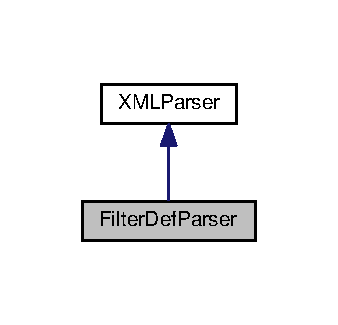
\includegraphics[width=162pt]{classFilterDefParser__inherit__graph}
\end{center}
\end{figure}


Collaboration diagram for Filter\+Def\+Parser\+:
\nopagebreak
\begin{figure}[H]
\begin{center}
\leavevmode
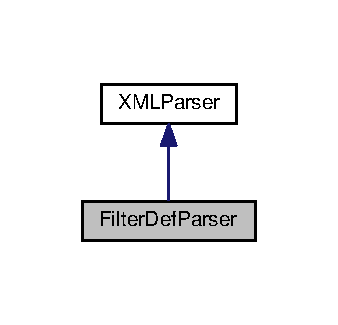
\includegraphics[width=162pt]{classFilterDefParser__coll__graph}
\end{center}
\end{figure}
\subsection*{Public Member Functions}
\begin{DoxyCompactItemize}
\item 
\mbox{\Hypertarget{classFilterDefParser_a3109e15681a4a9bcaaf9bef009ad34e6}\label{classFilterDefParser_a3109e15681a4a9bcaaf9bef009ad34e6}} 
{\bfseries Filter\+Def\+Parser} (string fname=\char`\"{}\char`\"{})
\item 
\mbox{\Hypertarget{classFilterDefParser_a14269618b595162814ac5c62a98f3c36}\label{classFilterDefParser_a14269618b595162814ac5c62a98f3c36}} 
virtual void \hyperlink{classFilterDefParser_a14269618b595162814ac5c62a98f3c36}{parse} (filter\+Def\+List\+\_\+t $\ast$list)
\begin{DoxyCompactList}\small\item\em add parsed filter definitions to list \end{DoxyCompactList}\end{DoxyCompactItemize}
\subsection*{Additional Inherited Members}


The documentation for this class was generated from the following files\+:\begin{DoxyCompactItemize}
\item 
include/Filter\+Def\+Parser.\+h\item 
src/Filter\+Def\+Parser.\+cpp\end{DoxyCompactItemize}

\hypertarget{structfilterValItem__t}{}\section{filter\+Val\+Item\+\_\+t Struct Reference}
\label{structfilterValItem__t}\index{filter\+Val\+Item\+\_\+t@{filter\+Val\+Item\+\_\+t}}


filter value  




{\ttfamily \#include $<$Filter\+Val\+Parser.\+h$>$}

\subsection*{Public Attributes}
\begin{DoxyCompactItemize}
\item 
\mbox{\Hypertarget{structfilterValItem__t_a89b779fa37fbf6ef52c28c37066ad5c9}\label{structfilterValItem__t_a89b779fa37fbf6ef52c28c37066ad5c9}} 
string {\bfseries name}
\item 
\mbox{\Hypertarget{structfilterValItem__t_a8ce4cc79957542c0de56856c29672679}\label{structfilterValItem__t_a8ce4cc79957542c0de56856c29672679}} 
string {\bfseries type}
\item 
\mbox{\Hypertarget{structfilterValItem__t_aba15c2104fa75c13c6bd63d4611a6486}\label{structfilterValItem__t_aba15c2104fa75c13c6bd63d4611a6486}} 
string {\bfseries svalue}
\end{DoxyCompactItemize}


\subsection{Detailed Description}
filter value 

The documentation for this struct was generated from the following file\+:\begin{DoxyCompactItemize}
\item 
include/Filter\+Val\+Parser.\+h\end{DoxyCompactItemize}

\hypertarget{classFilterValParser}{}\section{Filter\+Val\+Parser Class Reference}
\label{classFilterValParser}\index{Filter\+Val\+Parser@{Filter\+Val\+Parser}}


Inheritance diagram for Filter\+Val\+Parser\+:
\nopagebreak
\begin{figure}[H]
\begin{center}
\leavevmode
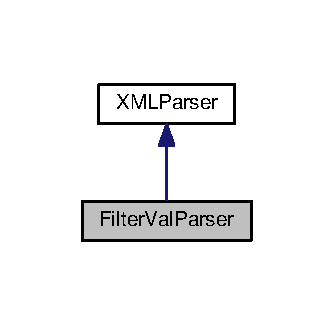
\includegraphics[width=160pt]{classFilterValParser__inherit__graph}
\end{center}
\end{figure}


Collaboration diagram for Filter\+Val\+Parser\+:
\nopagebreak
\begin{figure}[H]
\begin{center}
\leavevmode
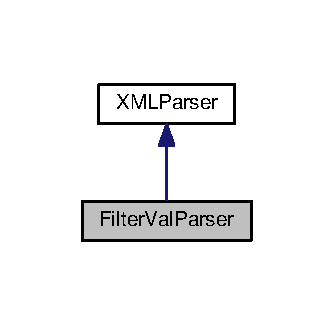
\includegraphics[width=160pt]{classFilterValParser__coll__graph}
\end{center}
\end{figure}
\subsection*{Public Member Functions}
\begin{DoxyCompactItemize}
\item 
\mbox{\Hypertarget{classFilterValParser_a700b6e94b751d4701f68d661a0f7c9ad}\label{classFilterValParser_a700b6e94b751d4701f68d661a0f7c9ad}} 
{\bfseries Filter\+Val\+Parser} (string fname)
\item 
\mbox{\Hypertarget{classFilterValParser_a054b191942c507d50a9be3ffafe685fd}\label{classFilterValParser_a054b191942c507d50a9be3ffafe685fd}} 
virtual void \hyperlink{classFilterValParser_a054b191942c507d50a9be3ffafe685fd}{parse} (filter\+Val\+List\+\_\+t $\ast$list)
\begin{DoxyCompactList}\small\item\em add parsed filter values to list \end{DoxyCompactList}\end{DoxyCompactItemize}
\subsection*{Additional Inherited Members}


The documentation for this class was generated from the following files\+:\begin{DoxyCompactItemize}
\item 
include/Filter\+Val\+Parser.\+h\item 
src/Filter\+Val\+Parser.\+cpp\end{DoxyCompactItemize}

\hypertarget{classFilterValue}{}\section{Filter\+Value Class Reference}
\label{classFilterValue}\index{Filter\+Value@{Filter\+Value}}
\subsection*{Public Member Functions}
\begin{DoxyCompactItemize}
\item 
\mbox{\Hypertarget{classFilterValue_afd9ace492d5ea61bf43abd1657dddb9d}\label{classFilterValue_afd9ace492d5ea61bf43abd1657dddb9d}} 
{\bfseries Filter\+Value} (string type, string value)
\item 
\mbox{\Hypertarget{classFilterValue_ace83c5669d4e07203202ae3431c7f3dd}\label{classFilterValue_ace83c5669d4e07203202ae3431c7f3dd}} 
string {\bfseries get\+String} ()
\item 
\mbox{\Hypertarget{classFilterValue_add166f01876f2b29be96165c9653a9de}\label{classFilterValue_add166f01876f2b29be96165c9653a9de}} 
int {\bfseries get\+Len} ()
\item 
\mbox{\Hypertarget{classFilterValue_a4364d94e9f2397d9b8ee29d7a729fe6c}\label{classFilterValue_a4364d94e9f2397d9b8ee29d7a729fe6c}} 
unsigned char $\ast$ {\bfseries get\+Value} ()
\item 
\mbox{\Hypertarget{classFilterValue_a3182fbb2edc32afad2c7c99bc262481b}\label{classFilterValue_a3182fbb2edc32afad2c7c99bc262481b}} 
string {\bfseries get\+Type} ()
\end{DoxyCompactItemize}
\subsection*{Static Public Member Functions}
\begin{DoxyCompactItemize}
\item 
\mbox{\Hypertarget{classFilterValue_a835706c98ea56790dab2b15cc3951a76}\label{classFilterValue_a835706c98ea56790dab2b15cc3951a76}} 
static int \hyperlink{classFilterValue_a835706c98ea56790dab2b15cc3951a76}{get\+Type\+Length} (string type)
\begin{DoxyCompactList}\small\item\em get length by type (for all fixed types) \end{DoxyCompactList}\end{DoxyCompactItemize}


The documentation for this class was generated from the following files\+:\begin{DoxyCompactItemize}
\item 
include/Filter\+Value.\+h\item 
src/Filter\+Value.\+cpp\end{DoxyCompactItemize}

\hypertarget{classGetInfoEvent}{}\section{Get\+Info\+Event Class Reference}
\label{classGetInfoEvent}\index{Get\+Info\+Event@{Get\+Info\+Event}}


Inheritance diagram for Get\+Info\+Event\+:
\nopagebreak
\begin{figure}[H]
\begin{center}
\leavevmode
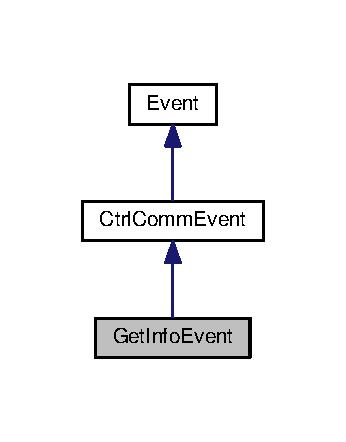
\includegraphics[width=166pt]{classGetInfoEvent__inherit__graph}
\end{center}
\end{figure}


Collaboration diagram for Get\+Info\+Event\+:
\nopagebreak
\begin{figure}[H]
\begin{center}
\leavevmode
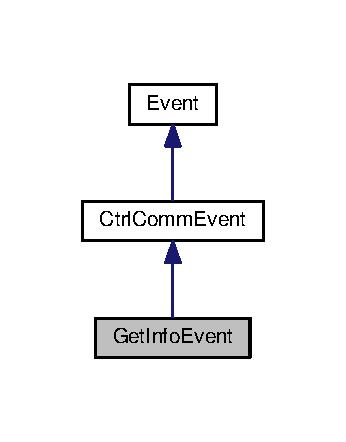
\includegraphics[width=166pt]{classGetInfoEvent__coll__graph}
\end{center}
\end{figure}
\subsection*{Public Member Functions}
\begin{DoxyCompactItemize}
\item 
\mbox{\Hypertarget{classGetInfoEvent_aadeef49fad32587ee4cf8642315222b3}\label{classGetInfoEvent_aadeef49fad32587ee4cf8642315222b3}} 
{\bfseries Get\+Info\+Event} (info\+List\+\_\+t $\ast$i)
\item 
\mbox{\Hypertarget{classGetInfoEvent_ae48faba56cacad3f16c8a39abfef180d}\label{classGetInfoEvent_ae48faba56cacad3f16c8a39abfef180d}} 
info\+List\+\_\+t $\ast$ {\bfseries get\+Infos} ()
\end{DoxyCompactItemize}


The documentation for this class was generated from the following file\+:\begin{DoxyCompactItemize}
\item 
include/\hyperlink{Event_8h}{Event.\+h}\end{DoxyCompactItemize}

\hypertarget{classGetModInfoEvent}{}\section{Get\+Mod\+Info\+Event Class Reference}
\label{classGetModInfoEvent}\index{Get\+Mod\+Info\+Event@{Get\+Mod\+Info\+Event}}


Inheritance diagram for Get\+Mod\+Info\+Event\+:
\nopagebreak
\begin{figure}[H]
\begin{center}
\leavevmode
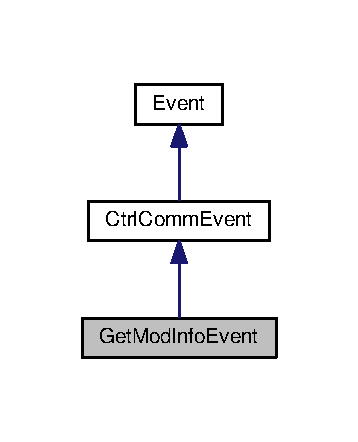
\includegraphics[width=172pt]{classGetModInfoEvent__inherit__graph}
\end{center}
\end{figure}


Collaboration diagram for Get\+Mod\+Info\+Event\+:
\nopagebreak
\begin{figure}[H]
\begin{center}
\leavevmode
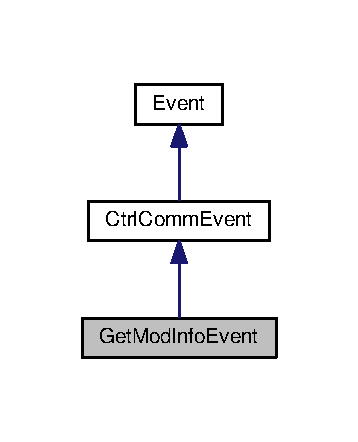
\includegraphics[width=172pt]{classGetModInfoEvent__coll__graph}
\end{center}
\end{figure}
\subsection*{Public Member Functions}
\begin{DoxyCompactItemize}
\item 
\mbox{\Hypertarget{classGetModInfoEvent_a39bb2be93dba7c6eb3edc2b5c09e536b}\label{classGetModInfoEvent_a39bb2be93dba7c6eb3edc2b5c09e536b}} 
{\bfseries Get\+Mod\+Info\+Event} (string modulename)
\item 
\mbox{\Hypertarget{classGetModInfoEvent_adb5ca4ffac0dbb5f71f01a98a796858e}\label{classGetModInfoEvent_adb5ca4ffac0dbb5f71f01a98a796858e}} 
string {\bfseries get\+Mod\+Name} ()
\end{DoxyCompactItemize}


The documentation for this class was generated from the following file\+:\begin{DoxyCompactItemize}
\item 
include/\hyperlink{Event_8h}{Event.\+h}\end{DoxyCompactItemize}

\hypertarget{structinfo__t}{}\section{info\+\_\+t Struct Reference}
\label{structinfo__t}\index{info\+\_\+t@{info\+\_\+t}}


type and value of a single meter info  




{\ttfamily \#include $<$Quality\+Manager\+Info.\+h$>$}

\subsection*{Public Member Functions}
\begin{DoxyCompactItemize}
\item 
\mbox{\Hypertarget{structinfo__t_a8e5a523c323d595e486c4b29f0bbe5c8}\label{structinfo__t_a8e5a523c323d595e486c4b29f0bbe5c8}} 
{\bfseries info\+\_\+t} (info\+Type\+\_\+t t, string p=\char`\"{}\char`\"{})
\end{DoxyCompactItemize}
\subsection*{Public Attributes}
\begin{DoxyCompactItemize}
\item 
\mbox{\Hypertarget{structinfo__t_aff97eaf43d6cea77eb92080edd134d7c}\label{structinfo__t_aff97eaf43d6cea77eb92080edd134d7c}} 
info\+Type\+\_\+t {\bfseries type}
\item 
\mbox{\Hypertarget{structinfo__t_a07e951effa1f491d74ed6a31eab77412}\label{structinfo__t_a07e951effa1f491d74ed6a31eab77412}} 
string {\bfseries param}
\end{DoxyCompactItemize}


\subsection{Detailed Description}
type and value of a single meter info 

The documentation for this struct was generated from the following file\+:\begin{DoxyCompactItemize}
\item 
include/Quality\+Manager\+Info.\+h\end{DoxyCompactItemize}

\hypertarget{classLogger}{}\section{Logger Class Reference}
\label{classLogger}\index{Logger@{Logger}}


provides logging of text messages to logging channels (files)  




{\ttfamily \#include $<$Logger.\+h$>$}

\subsection*{Public Member Functions}
\begin{DoxyCompactItemize}
\item 
\mbox{\Hypertarget{classLogger_a5a9c615a5e76e3ddd46825aa6d70bb79}\label{classLogger_a5a9c615a5e76e3ddd46825aa6d70bb79}} 
void \hyperlink{classLogger_a5a9c615a5e76e3ddd46825aa6d70bb79}{set\+Default\+Logfile} (string fname)
\begin{DoxyCompactList}\small\item\em set the log file which is used if no log file in explicitly given when opening a new channel \end{DoxyCompactList}\item 
\mbox{\Hypertarget{classLogger_acb668a9e186a25fbaad2e4af6d1ed00a}\label{classLogger_acb668a9e186a25fbaad2e4af6d1ed00a}} 
\hyperlink{classLogger_acb668a9e186a25fbaad2e4af6d1ed00a}{$\sim$\+Logger} ()
\begin{DoxyCompactList}\small\item\em destroys a message logger object, closes all open message channels (files) \end{DoxyCompactList}\item 
\mbox{\Hypertarget{classLogger_aa2e69cea8f4c129980f843c02e2279dd}\label{classLogger_aa2e69cea8f4c129980f843c02e2279dd}} 
void \hyperlink{classLogger_aa2e69cea8f4c129980f843c02e2279dd}{set\+Threaded} (int thr)
\begin{DoxyCompactList}\small\item\em set value of threading flag (see above) \end{DoxyCompactList}\item 
\mbox{\Hypertarget{classLogger_a5cc08473729523bb4bde48459f2ac468}\label{classLogger_a5cc08473729523bb4bde48459f2ac468}} 
void \hyperlink{classLogger_a5cc08473729523bb4bde48459f2ac468}{flush} ()
\begin{DoxyCompactList}\small\item\em flush all logging channels (does not close files) \end{DoxyCompactList}\item 
\mbox{\Hypertarget{classLogger_a76737728e58470cc99536839d6fbd631}\label{classLogger_a76737728e58470cc99536839d6fbd631}} 
void \hyperlink{classLogger_a76737728e58470cc99536839d6fbd631}{set\+Log\+Level} (int level)
\begin{DoxyCompactList}\small\item\em set the maximum logging level, higher levels will not be shown \end{DoxyCompactList}\item 
int \hyperlink{classLogger_a61e5d07bd9b1fd3296e737063d9e1809}{create\+Channel} (const string prefix=string(\char`\"{}\char`\"{}), const string name=string(\char`\"{}\char`\"{}), int newlog=1)
\begin{DoxyCompactList}\small\item\em assign a channel number to a file \end{DoxyCompactList}\item 
\mbox{\Hypertarget{classLogger_ae0584bd848e6f8beefbdad3f5f1d614c}\label{classLogger_ae0584bd848e6f8beefbdad3f5f1d614c}} 
int \hyperlink{classLogger_ae0584bd848e6f8beefbdad3f5f1d614c}{move\+Channels} (string ofname, string nfname, int newlog=1)
\begin{DoxyCompactList}\small\item\em rename (move) the currently used default logfile \end{DoxyCompactList}\item 
void \hyperlink{classLogger_a3277d0171f23be48ef40d86a01786284}{log} (int level, int channel, const char $\ast$fmt,...)
\begin{DoxyCompactList}\small\item\em logs a textual message to a channel \end{DoxyCompactList}\item 
\mbox{\Hypertarget{classLogger_a5156a9f382bb302b678e484c0ed7f2ef}\label{classLogger_a5156a9f382bb302b678e484c0ed7f2ef}} 
void {\bfseries log} (int channel, const char $\ast$fmt,...)
\item 
\mbox{\Hypertarget{classLogger_a07a7ccd017f70af90b52440c8c4b6a19}\label{classLogger_a07a7ccd017f70af90b52440c8c4b6a19}} 
void {\bfseries clog} (int channel, const char $\ast$fmt,...)
\item 
\mbox{\Hypertarget{classLogger_a87d34dedccbfbd0526cb1e0f352dfca2}\label{classLogger_a87d34dedccbfbd0526cb1e0f352dfca2}} 
void {\bfseries wlog} (int channel, const char $\ast$fmt,...)
\item 
\mbox{\Hypertarget{classLogger_aced539367fd2e477df2b78ab92e22e7f}\label{classLogger_aced539367fd2e477df2b78ab92e22e7f}} 
void {\bfseries elog} (int channel, const char $\ast$fmt,...)
\item 
\mbox{\Hypertarget{classLogger_a33ee464177bc7939cca0ae3ee28985d6}\label{classLogger_a33ee464177bc7939cca0ae3ee28985d6}} 
void {\bfseries dlog} (int channel, const char $\ast$fmt,...)
\item 
\mbox{\Hypertarget{classLogger_a44533b6fdd9f1f0d7730d77449e87985}\label{classLogger_a44533b6fdd9f1f0d7730d77449e87985}} 
void {\bfseries elog} (int channel, \hyperlink{classError}{Error} \&e)
\item 
\mbox{\Hypertarget{classLogger_a4477567175a3d8eb76130faf42ec865d}\label{classLogger_a4477567175a3d8eb76130faf42ec865d}} 
void {\bfseries elog} (int channel, \hyperlink{classProcError}{Proc\+Error} \&e)
\item 
\mbox{\Hypertarget{classLogger_afad2d6ca4c0725fa66e8d61e741d5776}\label{classLogger_afad2d6ca4c0725fa66e8d61e741d5776}} 
void \hyperlink{classLogger_afad2d6ca4c0725fa66e8d61e741d5776}{dump} (ostream \&os)
\begin{DoxyCompactList}\small\item\em dump \hyperlink{classLogger}{Logger} object \end{DoxyCompactList}\end{DoxyCompactItemize}
\subsection*{Static Public Member Functions}
\begin{DoxyCompactItemize}
\item 
\mbox{\Hypertarget{classLogger_afec28ae6d7bdf8f6a0734cb20756de10}\label{classLogger_afec28ae6d7bdf8f6a0734cb20756de10}} 
static \hyperlink{classLogger}{Logger} $\ast$ \hyperlink{classLogger_afec28ae6d7bdf8f6a0734cb20756de10}{get\+Instance} ()
\begin{DoxyCompactList}\small\item\em get access to the one and only \hyperlink{classLogger}{Logger} instance \end{DoxyCompactList}\end{DoxyCompactItemize}


\subsection{Detailed Description}
provides logging of text messages to logging channels (files) 

the \hyperlink{classLogger}{Logger} class is used to hold a number of F\+I\+L\+E$\ast$ for files in which logging of messages is to be done ~\newline
so you only need to have one global \hyperlink{classLogger}{Logger} object lying around ~\newline
~\newline
usage\+: ~\newline
create a \hyperlink{classLogger}{Logger} object ~\newline
assign a logging channel (number) to a file (filename) ~\newline
log messages to that channel (fprintf like syntax) 

\subsection{Member Function Documentation}
\mbox{\Hypertarget{classLogger_a61e5d07bd9b1fd3296e737063d9e1809}\label{classLogger_a61e5d07bd9b1fd3296e737063d9e1809}} 
\index{Logger@{Logger}!create\+Channel@{create\+Channel}}
\index{create\+Channel@{create\+Channel}!Logger@{Logger}}
\subsubsection{\texorpdfstring{create\+Channel()}{createChannel()}}
{\footnotesize\ttfamily int Logger\+::create\+Channel (\begin{DoxyParamCaption}\item[{const string}]{prefix = {\ttfamily string(\char`\"{}\char`\"{})},  }\item[{const string}]{name = {\ttfamily string(\char`\"{}\char`\"{})},  }\item[{int}]{newlog = {\ttfamily 1} }\end{DoxyParamCaption})}



assign a channel number to a file 

the file will be opened for appending text and each message logged to that channel will be written to that file ~\newline
the file will be opened for appending in line buffered mode

\begin{DoxyItemize}
\item {\ttfamily prefix} -\/ text to prepend to each message logged via this channel \item {\ttfamily name} -\/ name of file to appends messages to (optional), if unspecified default log file is used \item {\ttfamily newlog} -\/ remove log file first if =1, else append to file \end{DoxyItemize}
\mbox{\Hypertarget{classLogger_a3277d0171f23be48ef40d86a01786284}\label{classLogger_a3277d0171f23be48ef40d86a01786284}} 
\index{Logger@{Logger}!log@{log}}
\index{log@{log}!Logger@{Logger}}
\subsubsection{\texorpdfstring{log()}{log()}}
{\footnotesize\ttfamily void Logger\+::log (\begin{DoxyParamCaption}\item[{int}]{level,  }\item[{int}]{channel,  }\item[{const char $\ast$}]{fmt,  }\item[{}]{... }\end{DoxyParamCaption})}



logs a textual message to a channel 

the given text will be written to the file associated with the specified channel prefixed with that channels prefix string ~\newline
arguments after the format string are treated in a printf manner ~\newline
a newline written after the format string

\begin{DoxyItemize}
\item {\ttfamily channel} -\/ number of logging channel \item {\ttfamily fmt} -\/ printf like format string \item {\ttfamily }... -\/ additional arguments for printing\end{DoxyItemize}

\begin{DoxyExceptions}{Exceptions}
{\em \hyperlink{classError}{Error},get\+Error()} & can result in\+:
\begin{DoxyItemize}
\item \char`\"{}illegal channel number\char`\"{}
\item \char`\"{}channel not yet assigned\char`\"{}
\item \char`\"{}error writing to file\char`\"{} 
\end{DoxyItemize}\\
\hline
\end{DoxyExceptions}


The documentation for this class was generated from the following files\+:\begin{DoxyCompactItemize}
\item 
include/\hyperlink{Logger_8h}{Logger.\+h}\item 
src/Logger.\+cpp\end{DoxyCompactItemize}

\hypertarget{structltarg}{}\section{ltarg Struct Reference}
\label{structltarg}\index{ltarg@{ltarg}}


sort command line options alphabetically\+: a,A,b,B,c,D etc.  




{\ttfamily \#include $<$Command\+Line\+Args.\+h$>$}

\subsection*{Public Member Functions}
\begin{DoxyCompactItemize}
\item 
\mbox{\Hypertarget{structltarg_a87b6eddc57c2a991373e0bda64910bbd}\label{structltarg_a87b6eddc57c2a991373e0bda64910bbd}} 
bool {\bfseries operator()} (const char a1, const char a2) const
\end{DoxyCompactItemize}


\subsection{Detailed Description}
sort command line options alphabetically\+: a,A,b,B,c,D etc. 

The documentation for this struct was generated from the following file\+:\begin{DoxyCompactItemize}
\item 
include/\hyperlink{CommandLineArgs_8h}{Command\+Line\+Args.\+h}\end{DoxyCompactItemize}

\hypertarget{structltfd}{}\section{ltfd Struct Reference}
\label{structltfd}\index{ltfd@{ltfd}}


reverse sort operator according to fd  




{\ttfamily \#include $<$Quality\+Manager\+Component.\+h$>$}

\subsection*{Public Member Functions}
\begin{DoxyCompactItemize}
\item 
\mbox{\Hypertarget{structltfd_a4b7eb54c1de2870c5b34fc6f73827a4f}\label{structltfd_a4b7eb54c1de2870c5b34fc6f73827a4f}} 
bool {\bfseries operator()} (const \hyperlink{structfd__t}{fd\+\_\+t} f1, const \hyperlink{structfd__t}{fd\+\_\+t} f2) const
\end{DoxyCompactItemize}


\subsection{Detailed Description}
reverse sort operator according to fd 

The documentation for this struct was generated from the following file\+:\begin{DoxyCompactItemize}
\item 
include/\hyperlink{QualityManagerComponent_8h}{Quality\+Manager\+Component.\+h}\end{DoxyCompactItemize}

\hypertarget{structlttv}{}\section{lttv Struct Reference}
\label{structlttv}\index{lttv@{lttv}}


comparison operator for events  




{\ttfamily \#include $<$Event\+Scheduler.\+h$>$}

\subsection*{Public Member Functions}
\begin{DoxyCompactItemize}
\item 
\mbox{\Hypertarget{structlttv_a2f1845392453da6f88f8c0038557290d}\label{structlttv_a2f1845392453da6f88f8c0038557290d}} 
bool {\bfseries operator()} (const struct timeval t1, const struct timeval t2) const
\end{DoxyCompactItemize}


\subsection{Detailed Description}
comparison operator for events 

The documentation for this struct was generated from the following file\+:\begin{DoxyCompactItemize}
\item 
include/\hyperlink{EventScheduler_8h}{Event\+Scheduler.\+h}\end{DoxyCompactItemize}

\hypertarget{classMAPIRuleParser}{}\section{M\+A\+P\+I\+Rule\+Parser Class Reference}
\label{classMAPIRuleParser}\index{M\+A\+P\+I\+Rule\+Parser@{M\+A\+P\+I\+Rule\+Parser}}


parser for A\+PI text rule syntax  




{\ttfamily \#include $<$M\+A\+P\+I\+Rule\+Parser.\+h$>$}

\subsection*{Public Member Functions}
\begin{DoxyCompactItemize}
\item 
\mbox{\Hypertarget{classMAPIRuleParser_a07739a5e373e83dcd185395a6ed314b2}\label{classMAPIRuleParser_a07739a5e373e83dcd185395a6ed314b2}} 
{\bfseries M\+A\+P\+I\+Rule\+Parser} (string fname)
\item 
\mbox{\Hypertarget{classMAPIRuleParser_aa57dd2fec819cc49f4456c4e1583f0ba}\label{classMAPIRuleParser_aa57dd2fec819cc49f4456c4e1583f0ba}} 
{\bfseries M\+A\+P\+I\+Rule\+Parser} (char $\ast$b, int l)
\item 
\mbox{\Hypertarget{classMAPIRuleParser_a9dd9992ed6cbebddf20e0ddbb6c16339}\label{classMAPIRuleParser_a9dd9992ed6cbebddf20e0ddbb6c16339}} 
virtual void \hyperlink{classMAPIRuleParser_a9dd9992ed6cbebddf20e0ddbb6c16339}{parse} (filter\+Def\+List\+\_\+t $\ast$filters, filter\+Val\+List\+\_\+t $\ast$filter\+Vals, \hyperlink{RuleFileParser_8h_a7d5bb94bb17a8a1d92db2a89a0cc96d1}{rule\+D\+B\+\_\+t} $\ast$rules, \hyperlink{classRuleIdSource}{Rule\+Id\+Source} $\ast$id\+Source)
\begin{DoxyCompactList}\small\item\em parse given rules and add parsed rules to rules \end{DoxyCompactList}\end{DoxyCompactItemize}


\subsection{Detailed Description}
parser for A\+PI text rule syntax 

The documentation for this class was generated from the following files\+:\begin{DoxyCompactItemize}
\item 
include/M\+A\+P\+I\+Rule\+Parser.\+h\item 
src/M\+A\+P\+I\+Rule\+Parser.\+cpp\end{DoxyCompactItemize}

\hypertarget{structmetaData__t}{}\section{meta\+Data\+\_\+t Struct Reference}
\label{structmetaData__t}\index{meta\+Data\+\_\+t@{meta\+Data\+\_\+t}}
\subsection*{Public Attributes}
\begin{DoxyCompactItemize}
\item 
\mbox{\Hypertarget{structmetaData__t_a2342310924daa73d95516c4de4577f65}\label{structmetaData__t_a2342310924daa73d95516c4de4577f65}} 
unsigned long {\bfseries tv\+\_\+sec}
\item 
\mbox{\Hypertarget{structmetaData__t_a73a992c06df404ecdd5329ac2cbd4184}\label{structmetaData__t_a73a992c06df404ecdd5329ac2cbd4184}} 
unsigned long {\bfseries tv\+\_\+usec}
\item 
\mbox{\Hypertarget{structmetaData__t_a83e27493d1b587ccc69841f248f8792b}\label{structmetaData__t_a83e27493d1b587ccc69841f248f8792b}} 
char {\bfseries indev\+\_\+name} \mbox{[}255\mbox{]}
\item 
\mbox{\Hypertarget{structmetaData__t_a562a3476e5b43e4dfa3bf3ac713c552e}\label{structmetaData__t_a562a3476e5b43e4dfa3bf3ac713c552e}} 
char {\bfseries outdev\+\_\+name} \mbox{[}255\mbox{]}
\item 
\mbox{\Hypertarget{structmetaData__t_a60d44370774b3c26d84f22f9178eff7f}\label{structmetaData__t_a60d44370774b3c26d84f22f9178eff7f}} 
size\+\_\+t {\bfseries cap\+\_\+len}
\item 
\mbox{\Hypertarget{structmetaData__t_a261d19a12920810a456aa4f226471f57}\label{structmetaData__t_a261d19a12920810a456aa4f226471f57}} 
size\+\_\+t {\bfseries len}
\item 
\mbox{\Hypertarget{structmetaData__t_a924f583ec0509070c680d617efa93c7f}\label{structmetaData__t_a924f583ec0509070c680d617efa93c7f}} 
int {\bfseries offs} \mbox{[}4\mbox{]}
\item 
\mbox{\Hypertarget{structmetaData__t_a76b2be218e05f422ef10d0a7c5269886}\label{structmetaData__t_a76b2be218e05f422ef10d0a7c5269886}} 
int {\bfseries layers} \mbox{[}4\mbox{]}
\item 
\mbox{\Hypertarget{structmetaData__t_ae4d1c9a61cfd4ff105de96b26523469f}\label{structmetaData__t_ae4d1c9a61cfd4ff105de96b26523469f}} 
int {\bfseries reverse}
\item 
\mbox{\Hypertarget{structmetaData__t_a973a84a4d6d58d2d532eda96c4e82f2d}\label{structmetaData__t_a973a84a4d6d58d2d532eda96c4e82f2d}} 
unsigned short {\bfseries match\+\_\+cnt}
\item 
\mbox{\Hypertarget{structmetaData__t_a5dafc371fd326818994b58f1554cf481}\label{structmetaData__t_a5dafc371fd326818994b58f1554cf481}} 
unsigned int {\bfseries match} \mbox{[}M\+A\+X\+\_\+\+R\+U\+L\+E\+S\+\_\+\+M\+A\+T\+CH\mbox{]}
\item 
\mbox{\Hypertarget{structmetaData__t_a93200edb75f0b6fed9285ee04581a847}\label{structmetaData__t_a93200edb75f0b6fed9285ee04581a847}} 
unsigned char {\bfseries payload} \mbox{[}1\mbox{]}
\end{DoxyCompactItemize}


The documentation for this struct was generated from the following file\+:\begin{DoxyCompactItemize}
\item 
include/\hyperlink{metadata_8h}{metadata.\+h}\end{DoxyCompactItemize}

\hypertarget{structMIME}{}\section{M\+I\+ME Struct Reference}
\label{structMIME}\index{M\+I\+ME@{M\+I\+ME}}
\subsection*{Public Attributes}
\begin{DoxyCompactItemize}
\item 
\mbox{\Hypertarget{structMIME_a601909559c56e6453ae5cfc02453cc53}\label{structMIME_a601909559c56e6453ae5cfc02453cc53}} 
char {\bfseries ext} \mbox{[}8\mbox{]}
\item 
\mbox{\Hypertarget{structMIME_a827c7c2f660ab4ce4f25f96cf456591f}\label{structMIME_a827c7c2f660ab4ce4f25f96cf456591f}} 
char {\bfseries type} \mbox{[}64\mbox{]}
\end{DoxyCompactItemize}


The documentation for this struct was generated from the following file\+:\begin{DoxyCompactItemize}
\item 
lib/httpd/\hyperlink{mime_8c}{mime.\+c}\end{DoxyCompactItemize}

\hypertarget{classModule}{}\section{Module Class Reference}
\label{classModule}\index{Module@{Module}}


super class for the loadable modules (for processing and export)  




{\ttfamily \#include $<$Module.\+h$>$}



Inheritance diagram for Module\+:
\nopagebreak
\begin{figure}[H]
\begin{center}
\leavevmode
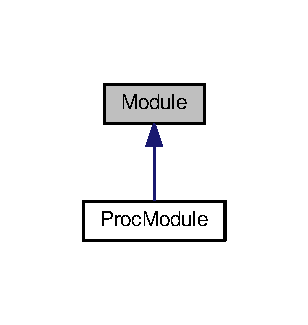
\includegraphics[width=148pt]{classModule__inherit__graph}
\end{center}
\end{figure}
\subsection*{Public Member Functions}
\begin{DoxyCompactItemize}
\item 
\mbox{\Hypertarget{classModule_a2b4410ea8c8158eb4ccd32621ac3ac44}\label{classModule_a2b4410ea8c8158eb4ccd32621ac3ac44}} 
int \hyperlink{classModule_a2b4410ea8c8158eb4ccd32621ac3ac44}{link} ()
\begin{DoxyCompactList}\small\item\em increase module usage counter \end{DoxyCompactList}\item 
\mbox{\Hypertarget{classModule_a77961c31e38eed0460678e58b815ca9d}\label{classModule_a77961c31e38eed0460678e58b815ca9d}} 
int \hyperlink{classModule_a77961c31e38eed0460678e58b815ca9d}{unlink} ()
\begin{DoxyCompactList}\small\item\em decrease module usage counter \end{DoxyCompactList}\item 
\mbox{\Hypertarget{classModule_ae15cbc8e4cc023389220f6bc1573e79a}\label{classModule_ae15cbc8e4cc023389220f6bc1573e79a}} 
\hyperlink{Module_8h_acbeb44869400b78e5f4097d5c49fc093}{lib\+Handle\+\_\+t} {\bfseries get\+Lib} ()
\item 
\mbox{\Hypertarget{classModule_a94c2adde5e84aa06271287caa52582fd}\label{classModule_a94c2adde5e84aa06271287caa52582fd}} 
string {\bfseries get\+Mod\+Name} ()
\item 
\mbox{\Hypertarget{classModule_a17cd6df369ee653ebda1a7dd98ac80bd}\label{classModule_a17cd6df369ee653ebda1a7dd98ac80bd}} 
string {\bfseries get\+File\+Name} ()
\item 
\mbox{\Hypertarget{classModule_a88fb093ef0a9a2689d35c2a2df7903a9}\label{classModule_a88fb093ef0a9a2689d35c2a2df7903a9}} 
string {\bfseries get\+Own\+Name} ()
\item 
\mbox{\Hypertarget{classModule_a2cf459f20fb61bb1fde784852c0b4ae8}\label{classModule_a2cf459f20fb61bb1fde784852c0b4ae8}} 
void {\bfseries set\+Own\+Name} (string name)
\item 
\mbox{\Hypertarget{classModule_a86d4d45174189e9ee7226ec366a4ab4e}\label{classModule_a86d4d45174189e9ee7226ec366a4ab4e}} 
int {\bfseries get\+Refs} ()
\item 
\mbox{\Hypertarget{classModule_a658eb3f9f97a6ea60d5c21c73c711d3e}\label{classModule_a658eb3f9f97a6ea60d5c21c73c711d3e}} 
virtual int {\bfseries get\+Version} ()
\item 
\mbox{\Hypertarget{classModule_a0a0a9e897515df7ac9ab031015e3d352}\label{classModule_a0a0a9e897515df7ac9ab031015e3d352}} 
virtual string {\bfseries get\+Module\+Type} ()
\item 
\hyperlink{classModule_a431b07620991847651303e0f252e8285}{Module} (string libname, string filename, \hyperlink{Module_8h_acbeb44869400b78e5f4097d5c49fc093}{lib\+Handle\+\_\+t} libhandle)
\begin{DoxyCompactList}\small\item\em construct and initialize a \hyperlink{classModule}{Module} object \end{DoxyCompactList}\item 
\mbox{\Hypertarget{classModule_a7c9d9c096786d127590fdd8aa2b7d681}\label{classModule_a7c9d9c096786d127590fdd8aa2b7d681}} 
virtual \hyperlink{classModule_a7c9d9c096786d127590fdd8aa2b7d681}{$\sim$\+Module} ()
\begin{DoxyCompactList}\small\item\em destroy a \hyperlink{classModule}{Module} object, to be overloaded \end{DoxyCompactList}\item 
void $\ast$ \hyperlink{classModule_a4a9a9aa2518c2486e9bcb309277a1bf1}{load\+A\+PI} (string api\+Name)
\begin{DoxyCompactList}\small\item\em load A\+PI (block of module function references) \end{DoxyCompactList}\item 
void \hyperlink{classModule_a3394d69c34f70e6d54fcebcb22c2a2c2}{check\+Magic} (int magic)
\begin{DoxyCompactList}\small\item\em check magic number in module tries to read magic number from module lib file and check for correctness \end{DoxyCompactList}\item 
\mbox{\Hypertarget{classModule_a6f0917a69ba21d691c6b20a65369c6c6}\label{classModule_a6f0917a69ba21d691c6b20a65369c6c6}} 
void \hyperlink{classModule_a6f0917a69ba21d691c6b20a65369c6c6}{dump} (ostream \&os)
\begin{DoxyCompactList}\small\item\em dump a \hyperlink{classModule}{Module} object \end{DoxyCompactList}\end{DoxyCompactItemize}


\subsection{Detailed Description}
super class for the loadable modules (for processing and export) 

super class -\/ stores information about an loadbale module such as name, libhandle and reference counter 

\subsection{Constructor \& Destructor Documentation}
\mbox{\Hypertarget{classModule_a431b07620991847651303e0f252e8285}\label{classModule_a431b07620991847651303e0f252e8285}} 
\index{Module@{Module}!Module@{Module}}
\index{Module@{Module}!Module@{Module}}
\subsubsection{\texorpdfstring{Module()}{Module()}}
{\footnotesize\ttfamily Module\+::\+Module (\begin{DoxyParamCaption}\item[{string}]{libname,  }\item[{string}]{filename,  }\item[{\hyperlink{Module_8h_acbeb44869400b78e5f4097d5c49fc093}{lib\+Handle\+\_\+t}}]{libhandle }\end{DoxyParamCaption})}



construct and initialize a \hyperlink{classModule}{Module} object 

take the library handle of an evaluation module and retrieve all the other information (name, uid, function list) via this handle

\begin{DoxyItemize}
\item {\ttfamily libname} -\/ name of the evaluation module \item {\ttfamily filename} -\/ name of module including path and extension \item {\ttfamily libhandle} -\/ system handle for loaded library (see dlopen) \end{DoxyItemize}


\subsection{Member Function Documentation}
\mbox{\Hypertarget{classModule_a3394d69c34f70e6d54fcebcb22c2a2c2}\label{classModule_a3394d69c34f70e6d54fcebcb22c2a2c2}} 
\index{Module@{Module}!check\+Magic@{check\+Magic}}
\index{check\+Magic@{check\+Magic}!Module@{Module}}
\subsubsection{\texorpdfstring{check\+Magic()}{checkMagic()}}
{\footnotesize\ttfamily void Module\+::check\+Magic (\begin{DoxyParamCaption}\item[{int}]{magic }\end{DoxyParamCaption})}



check magic number in module tries to read magic number from module lib file and check for correctness 


\begin{DoxyExceptions}{Exceptions}
{\em \hyperlink{classError}{Error}} & in case magic number is not present or is wrong \\
\hline
\end{DoxyExceptions}
\mbox{\Hypertarget{classModule_a4a9a9aa2518c2486e9bcb309277a1bf1}\label{classModule_a4a9a9aa2518c2486e9bcb309277a1bf1}} 
\index{Module@{Module}!load\+A\+PI@{load\+A\+PI}}
\index{load\+A\+PI@{load\+A\+PI}!Module@{Module}}
\subsubsection{\texorpdfstring{load\+A\+P\+I()}{loadAPI()}}
{\footnotesize\ttfamily void $\ast$ Module\+::load\+A\+PI (\begin{DoxyParamCaption}\item[{string}]{api\+Name }\end{DoxyParamCaption})}



load A\+PI (block of module function references) 

this function queries the module for the block of module functions ( a struct storing function pointers to the module\textquotesingle{}s methods ) 

The documentation for this class was generated from the following files\+:\begin{DoxyCompactItemize}
\item 
include/\hyperlink{Module_8h}{Module.\+h}\item 
src/\hyperlink{Module_8cc}{Module.\+cc}\end{DoxyCompactItemize}

\hypertarget{classModuleLoader}{}\section{Module\+Loader Class Reference}
\label{classModuleLoader}\index{Module\+Loader@{Module\+Loader}}


load dynamic libraries and extract function pointers  




{\ttfamily \#include $<$Module\+Loader.\+h$>$}

\subsection*{Public Member Functions}
\begin{DoxyCompactItemize}
\item 
\hyperlink{classModuleLoader_ab7ab1224836096260ae1a325941fe24c}{Module\+Loader} (\hyperlink{classConfigManager}{Config\+Manager} $\ast$cnf, string basedir=\char`\"{}./\char`\"{}, string modules=\char`\"{}\char`\"{}, string channel\+Prefix=\char`\"{}\char`\"{}, string group=\char`\"{}\char`\"{})
\begin{DoxyCompactList}\small\item\em construct and initialize a \hyperlink{classModuleLoader}{Module\+Loader} object \end{DoxyCompactList}\item 
\hyperlink{classModuleLoader_a79d95bc9360ee001972bb1990d37b1a5}{$\sim$\+Module\+Loader} ()
\begin{DoxyCompactList}\small\item\em destroy a \hyperlink{classModuleLoader}{Module\+Loader} object \end{DoxyCompactList}\item 
\hyperlink{classModule}{Module} $\ast$ \hyperlink{classModuleLoader_a494036ae2850f065ea0676f5b2351093}{load\+Module} (string libname, int preload)
\begin{DoxyCompactList}\small\item\em load a metric module and make its functions available \end{DoxyCompactList}\item 
\hyperlink{classModule}{Module} $\ast$ \hyperlink{classModuleLoader_ac39cac913d2201252c2501664c9926f7}{get\+Module} (string libname)
\begin{DoxyCompactList}\small\item\em get the info block for a loaded metric module \end{DoxyCompactList}\item 
\mbox{\Hypertarget{classModuleLoader_a6768a60b55dc11cb5cc5aea2d7bb2a8d}\label{classModuleLoader_a6768a60b55dc11cb5cc5aea2d7bb2a8d}} 
string \hyperlink{classModuleLoader_a6768a60b55dc11cb5cc5aea2d7bb2a8d}{get\+Module\+Info\+X\+ML} (string modname)
\begin{DoxyCompactList}\small\item\em get xml description of module \end{DoxyCompactList}\item 
int \hyperlink{classModuleLoader_aa9dd4cbeb24b4a413a270c192bce95b4}{release\+Module} (\hyperlink{classModule}{Module} $\ast$minfo)
\begin{DoxyCompactList}\small\item\em decrement reference count to a loaded dynamic lobrary \end{DoxyCompactList}\item 
\hyperlink{structtypeInfo__t}{type\+Info\+\_\+t} $\ast$ \hyperlink{classModuleLoader_ac9828e3ed8c3ffa0b6bfb54dc43d5be3}{get\+Type\+Info} (string modname)
\begin{DoxyCompactList}\small\item\em get the runtime type information for a module \end{DoxyCompactList}\item 
\mbox{\Hypertarget{classModuleLoader_aeec24847fe646ce612720c657185e420}\label{classModuleLoader_aeec24847fe646ce612720c657185e420}} 
int {\bfseries get\+Version} (string modname)
\item 
void \hyperlink{classModuleLoader_ac3ddb6d3909749301dea325f1e820f2d}{write\+Type\+Info} (string modname)
\begin{DoxyCompactList}\small\item\em print export data type information \end{DoxyCompactList}\item 
\mbox{\Hypertarget{classModuleLoader_a6b23900d6a7316a3df2583854f41b1ed}\label{classModuleLoader_a6b23900d6a7316a3df2583854f41b1ed}} 
int \hyperlink{classModuleLoader_a6b23900d6a7316a3df2583854f41b1ed}{fetch\+Magic} (\hyperlink{Module_8h_acbeb44869400b78e5f4097d5c49fc093}{lib\+Handle\+\_\+t} lib\+Handle)
\begin{DoxyCompactList}\small\item\em fetch magic number from module lib file \end{DoxyCompactList}\item 
\mbox{\Hypertarget{classModuleLoader_af3bc48297a382f05a39d0f63adc7afe4}\label{classModuleLoader_af3bc48297a382f05a39d0f63adc7afe4}} 
string \hyperlink{classModuleLoader_af3bc48297a382f05a39d0f63adc7afe4}{get\+Info} ()
\begin{DoxyCompactList}\small\item\em F\+I\+X\+ME missing documentation. \end{DoxyCompactList}\item 
void \hyperlink{classModuleLoader_a863d9c602af7d21714d0096c57780af7}{dump} (ostream \&os)
\begin{DoxyCompactList}\small\item\em dump a \hyperlink{classModuleLoader}{Module\+Loader} object \end{DoxyCompactList}\item 
\mbox{\Hypertarget{classModuleLoader_a216786f53c44b08506a26e595ab40d38}\label{classModuleLoader_a216786f53c44b08506a26e595ab40d38}} 
int \hyperlink{classModuleLoader_a216786f53c44b08506a26e595ab40d38}{num\+Modules} ()
\begin{DoxyCompactList}\small\item\em return number of currently loaded modules \end{DoxyCompactList}\end{DoxyCompactItemize}


\subsection{Detailed Description}
load dynamic libraries and extract function pointers 

the \hyperlink{classModuleLoader}{Module\+Loader} class allows requesting of a dynamic library that is to be used. That Library will be loaded and it\textquotesingle{}s functions made available to the caller using the \hyperlink{classModuleLoader}{Module\+Loader} object. 

\subsection{Constructor \& Destructor Documentation}
\mbox{\Hypertarget{classModuleLoader_ab7ab1224836096260ae1a325941fe24c}\label{classModuleLoader_ab7ab1224836096260ae1a325941fe24c}} 
\index{Module\+Loader@{Module\+Loader}!Module\+Loader@{Module\+Loader}}
\index{Module\+Loader@{Module\+Loader}!Module\+Loader@{Module\+Loader}}
\subsubsection{\texorpdfstring{Module\+Loader()}{ModuleLoader()}}
{\footnotesize\ttfamily Module\+Loader\+::\+Module\+Loader (\begin{DoxyParamCaption}\item[{\hyperlink{classConfigManager}{Config\+Manager} $\ast$}]{cnf,  }\item[{string}]{basedir = {\ttfamily \char`\"{}./\char`\"{}},  }\item[{string}]{modules = {\ttfamily \char`\"{}\char`\"{}},  }\item[{string}]{channel\+Prefix = {\ttfamily \char`\"{}\char`\"{}},  }\item[{string}]{group = {\ttfamily \char`\"{}\char`\"{}} }\end{DoxyParamCaption})}



construct and initialize a \hyperlink{classModuleLoader}{Module\+Loader} object 

\begin{DoxyItemize}
\item {\ttfamily basedir} -\/ directory that contains libraries that can by loaded with subsequent calls to \hyperlink{classModuleLoader_ac39cac913d2201252c2501664c9926f7}{get\+Module()} \item {\ttfamily modules} -\/ names of metric modules separated by \char`\"{} \char`\"{} \end{DoxyItemize}
\mbox{\Hypertarget{classModuleLoader_a79d95bc9360ee001972bb1990d37b1a5}\label{classModuleLoader_a79d95bc9360ee001972bb1990d37b1a5}} 
\index{Module\+Loader@{Module\+Loader}!````~Module\+Loader@{$\sim$\+Module\+Loader}}
\index{````~Module\+Loader@{$\sim$\+Module\+Loader}!Module\+Loader@{Module\+Loader}}
\subsubsection{\texorpdfstring{$\sim$\+Module\+Loader()}{~ModuleLoader()}}
{\footnotesize\ttfamily Module\+Loader\+::$\sim$\+Module\+Loader (\begin{DoxyParamCaption}{ }\end{DoxyParamCaption})}



destroy a \hyperlink{classModuleLoader}{Module\+Loader} object 

this will close all dynamic libraries used by this \hyperlink{classModuleLoader}{Module\+Loader} (or at least decrement their reference counter if they are used otherwise) 

\subsection{Member Function Documentation}
\mbox{\Hypertarget{classModuleLoader_a863d9c602af7d21714d0096c57780af7}\label{classModuleLoader_a863d9c602af7d21714d0096c57780af7}} 
\index{Module\+Loader@{Module\+Loader}!dump@{dump}}
\index{dump@{dump}!Module\+Loader@{Module\+Loader}}
\subsubsection{\texorpdfstring{dump()}{dump()}}
{\footnotesize\ttfamily void Module\+Loader\+::dump (\begin{DoxyParamCaption}\item[{ostream \&}]{os }\end{DoxyParamCaption})}



dump a \hyperlink{classModuleLoader}{Module\+Loader} object 

display names of loaded libraries and the number of times they have been requested \mbox{\Hypertarget{classModuleLoader_ac39cac913d2201252c2501664c9926f7}\label{classModuleLoader_ac39cac913d2201252c2501664c9926f7}} 
\index{Module\+Loader@{Module\+Loader}!get\+Module@{get\+Module}}
\index{get\+Module@{get\+Module}!Module\+Loader@{Module\+Loader}}
\subsubsection{\texorpdfstring{get\+Module()}{getModule()}}
{\footnotesize\ttfamily \hyperlink{classModule}{Module} $\ast$ Module\+Loader\+::get\+Module (\begin{DoxyParamCaption}\item[{string}]{libname }\end{DoxyParamCaption})}



get the info block for a loaded metric module 

looks for a metric module with the specified name and returns an info block for this module

\begin{DoxyItemize}
\item {\ttfamily libname} -\/ name of the library \begin{DoxyReturn}{Returns}
a reference to a struct with pointers to all the functions of the Action \hyperlink{classModule}{Module} 
\end{DoxyReturn}

\begin{DoxyExceptions}{Exceptions}
{\em My\+Err} & in case the module is not available \\
\hline
\end{DoxyExceptions}
\end{DoxyItemize}
\mbox{\Hypertarget{classModuleLoader_ac9828e3ed8c3ffa0b6bfb54dc43d5be3}\label{classModuleLoader_ac9828e3ed8c3ffa0b6bfb54dc43d5be3}} 
\index{Module\+Loader@{Module\+Loader}!get\+Type\+Info@{get\+Type\+Info}}
\index{get\+Type\+Info@{get\+Type\+Info}!Module\+Loader@{Module\+Loader}}
\subsubsection{\texorpdfstring{get\+Type\+Info()}{getTypeInfo()}}
{\footnotesize\ttfamily \hyperlink{structtypeInfo__t}{type\+Info\+\_\+t} $\ast$ Module\+Loader\+::get\+Type\+Info (\begin{DoxyParamCaption}\item[{string}]{modname }\end{DoxyParamCaption})}



get the runtime type information for a module 

\begin{DoxyItemize}
\item {\ttfamily modname} -\/ name of the evaluation module \begin{DoxyReturn}{Returns}
the type information for the data exported by the requested evaluation module 
\end{DoxyReturn}
\end{DoxyItemize}
\mbox{\Hypertarget{classModuleLoader_a494036ae2850f065ea0676f5b2351093}\label{classModuleLoader_a494036ae2850f065ea0676f5b2351093}} 
\index{Module\+Loader@{Module\+Loader}!load\+Module@{load\+Module}}
\index{load\+Module@{load\+Module}!Module\+Loader@{Module\+Loader}}
\subsubsection{\texorpdfstring{load\+Module()}{loadModule()}}
{\footnotesize\ttfamily \hyperlink{classModule}{Module} $\ast$ Module\+Loader\+::load\+Module (\begin{DoxyParamCaption}\item[{string}]{libname,  }\item[{int}]{preload }\end{DoxyParamCaption})}



load a metric module and make its functions available 

tries to open a module and return a list of functions from it. The library has to include \textquotesingle{}Action\+Module.\+h\textquotesingle{} and needs to implement all functions given in \textquotesingle{}\hyperlink{ProcModuleInterface_8h}{Proc\+Module\+Interface.\+h}\textquotesingle{}

\begin{DoxyItemize}
\item {\ttfamily modname} -\/ name of the module \item {\ttfamily preload} -\/ load module instantly (not only on demand) if ==1 \begin{DoxyReturn}{Returns}
a reference to a struct with pointers to all the functions of the module 
\end{DoxyReturn}

\begin{DoxyExceptions}{Exceptions}
{\em \hyperlink{classError}{Error}} & in case the module is not available \\
\hline
\end{DoxyExceptions}
\end{DoxyItemize}
\mbox{\Hypertarget{classModuleLoader_aa9dd4cbeb24b4a413a270c192bce95b4}\label{classModuleLoader_aa9dd4cbeb24b4a413a270c192bce95b4}} 
\index{Module\+Loader@{Module\+Loader}!release\+Module@{release\+Module}}
\index{release\+Module@{release\+Module}!Module\+Loader@{Module\+Loader}}
\subsubsection{\texorpdfstring{release\+Module()}{releaseModule()}}
{\footnotesize\ttfamily int Module\+Loader\+::release\+Module (\begin{DoxyParamCaption}\item[{\hyperlink{classModule}{Module} $\ast$}]{minfo }\end{DoxyParamCaption})}



decrement reference count to a loaded dynamic lobrary 

reduce the link count of the given library by one. If the link count reaches zero by doing so, the library is unloaded.

\begin{DoxyItemize}
\item {\ttfamily minfo} -\/ pointer to module \end{DoxyItemize}
\mbox{\Hypertarget{classModuleLoader_ac3ddb6d3909749301dea325f1e820f2d}\label{classModuleLoader_ac3ddb6d3909749301dea325f1e820f2d}} 
\index{Module\+Loader@{Module\+Loader}!write\+Type\+Info@{write\+Type\+Info}}
\index{write\+Type\+Info@{write\+Type\+Info}!Module\+Loader@{Module\+Loader}}
\subsubsection{\texorpdfstring{write\+Type\+Info()}{writeTypeInfo()}}
{\footnotesize\ttfamily void Module\+Loader\+::write\+Type\+Info (\begin{DoxyParamCaption}\item[{string}]{modname }\end{DoxyParamCaption})}



print export data type information 

\begin{DoxyItemize}
\item {\ttfamily modname} -\/ name of the proc module \end{DoxyItemize}


The documentation for this class was generated from the following files\+:\begin{DoxyCompactItemize}
\item 
include/\hyperlink{ModuleLoader_8h}{Module\+Loader.\+h}\item 
src/\hyperlink{ModuleLoader_8cpp}{Module\+Loader.\+cpp}\end{DoxyCompactItemize}

\hypertarget{structopt__map}{}\section{opt\+\_\+map Struct Reference}
\label{structopt__map}\index{opt\+\_\+map@{opt\+\_\+map}}
\subsection*{Public Attributes}
\begin{DoxyCompactItemize}
\item 
\mbox{\Hypertarget{structopt__map_a882f881a898314cb4f25ec67224de6f7}\label{structopt__map_a882f881a898314cb4f25ec67224de6f7}} 
const char $\ast$ {\bfseries mcl}
\item 
\mbox{\Hypertarget{structopt__map_a56bc1ec14240258881e159160a79694c}\label{structopt__map_a56bc1ec14240258881e159160a79694c}} 
const char $\ast$ {\bfseries iptables}
\end{DoxyCompactItemize}


The documentation for this struct was generated from the following file\+:\begin{DoxyCompactItemize}
\item 
proc\+\_\+modules/\hyperlink{htb_8cpp}{htb.\+cpp}\end{DoxyCompactItemize}

\hypertarget{structoption}{}\section{option Struct Reference}
\label{structoption}\index{option@{option}}
\subsection*{Public Attributes}
\begin{DoxyCompactItemize}
\item 
\mbox{\Hypertarget{structoption_a92c850a23c7828c1dba453bf8d15e1f0}\label{structoption_a92c850a23c7828c1dba453bf8d15e1f0}} 
char $\ast$ {\bfseries name}
\item 
\mbox{\Hypertarget{structoption_a90d7ee9a51eea5c002682dbd0af149e4}\label{structoption_a90d7ee9a51eea5c002682dbd0af149e4}} 
int {\bfseries has\+\_\+arg}
\item 
\mbox{\Hypertarget{structoption_ab366eea5fe7be25c1928328ba715e353}\label{structoption_ab366eea5fe7be25c1928328ba715e353}} 
int $\ast$ {\bfseries flag}
\item 
\mbox{\Hypertarget{structoption_a13bd155ec3b405d29c41ab8d0793be11}\label{structoption_a13bd155ec3b405d29c41ab8d0793be11}} 
int {\bfseries val}
\end{DoxyCompactItemize}


The documentation for this struct was generated from the following file\+:\begin{DoxyCompactItemize}
\item 
lib/getopt\+\_\+long/getopt\+\_\+long.\+h\end{DoxyCompactItemize}

\hypertarget{classPageRepository}{}\section{Page\+Repository Class Reference}
\label{classPageRepository}\index{Page\+Repository@{Page\+Repository}}


stores H\+T\+ML pages (i.\+e. text strings) which can be found based on their U\+RI name (path + page-\/name)  




{\ttfamily \#include $<$Page\+Repository.\+h$>$}

\subsection*{Public Member Functions}
\begin{DoxyCompactItemize}
\item 
\mbox{\Hypertarget{classPageRepository_a3ba320211d1c61641a1105bb46322b3d}\label{classPageRepository_a3ba320211d1c61641a1105bb46322b3d}} 
void \hyperlink{classPageRepository_a3ba320211d1c61641a1105bb46322b3d}{add\+Page} (string url, string content)
\begin{DoxyCompactList}\small\item\em F\+I\+X\+ME document. \end{DoxyCompactList}\item 
\mbox{\Hypertarget{classPageRepository_a908993cca7ed7b8df0833d2fba444d14}\label{classPageRepository_a908993cca7ed7b8df0833d2fba444d14}} 
void {\bfseries add\+Page\+File} (string url, string filename)
\item 
\mbox{\Hypertarget{classPageRepository_a6731593d95cea84cf705d8ce6672c869}\label{classPageRepository_a6731593d95cea84cf705d8ce6672c869}} 
string {\bfseries get\+Page} (string url)
\item 
\mbox{\Hypertarget{classPageRepository_a4b59ed8a349dba67089ff8babecd324b}\label{classPageRepository_a4b59ed8a349dba67089ff8babecd324b}} 
string {\bfseries get\+File\+Name} (string url)
\end{DoxyCompactItemize}


\subsection{Detailed Description}
stores H\+T\+ML pages (i.\+e. text strings) which can be found based on their U\+RI name (path + page-\/name) 

The documentation for this class was generated from the following files\+:\begin{DoxyCompactItemize}
\item 
include/\hyperlink{PageRepository_8h}{Page\+Repository.\+h}\item 
src/Page\+Repository.\+cpp\end{DoxyCompactItemize}

\hypertarget{structparseReq__t}{}\section{parse\+Req\+\_\+t Struct Reference}
\label{structparseReq__t}\index{parse\+Req\+\_\+t@{parse\+Req\+\_\+t}}


command and parameter contained in a request  




{\ttfamily \#include $<$Ctrl\+Comm.\+h$>$}

\subsection*{Public Attributes}
\begin{DoxyCompactItemize}
\item 
\mbox{\Hypertarget{structparseReq__t_ad378450c6e9686f863a1d1bd98a9082d}\label{structparseReq__t_ad378450c6e9686f863a1d1bd98a9082d}} 
string {\bfseries comm}
\item 
\mbox{\Hypertarget{structparseReq__t_a21860319f5f68e387a086abb9a71027a}\label{structparseReq__t_a21860319f5f68e387a086abb9a71027a}} 
param\+List\+\_\+t {\bfseries params}
\end{DoxyCompactItemize}


\subsection{Detailed Description}
command and parameter contained in a request 

The documentation for this struct was generated from the following file\+:\begin{DoxyCompactItemize}
\item 
include/Ctrl\+Comm.\+h\end{DoxyCompactItemize}

\hypertarget{classParserFcts}{}\section{Parser\+Fcts Class Reference}
\label{classParserFcts}\index{Parser\+Fcts@{Parser\+Fcts}}
\subsection*{Static Public Member Functions}
\begin{DoxyCompactItemize}
\item 
\mbox{\Hypertarget{classParserFcts_a2eea6aa325dc6d2ebe9b509183ef1fe4}\label{classParserFcts_a2eea6aa325dc6d2ebe9b509183ef1fe4}} 
static long {\bfseries parse\+Long} (string s, long min=L\+O\+N\+G\+\_\+\+M\+IN, long max=L\+O\+N\+G\+\_\+\+M\+AX)
\item 
\mbox{\Hypertarget{classParserFcts_a32787caa043d964e5368f80a03a0632a}\label{classParserFcts_a32787caa043d964e5368f80a03a0632a}} 
static unsigned long {\bfseries parse\+U\+Long} (string s, unsigned long min=0, unsigned long max=U\+L\+O\+N\+G\+\_\+\+M\+AX)
\item 
\mbox{\Hypertarget{classParserFcts_a2d35300e2b8ebdb39bb26402af786a87}\label{classParserFcts_a2d35300e2b8ebdb39bb26402af786a87}} 
static long long {\bfseries parse\+L\+Long} (string s, long long min=L\+L\+O\+N\+G\+\_\+\+M\+IN, long long max=L\+L\+O\+N\+G\+\_\+\+M\+AX)
\item 
\mbox{\Hypertarget{classParserFcts_a18324a2102c2f085af647e698963dd7a}\label{classParserFcts_a18324a2102c2f085af647e698963dd7a}} 
static unsigned long long {\bfseries parse\+U\+L\+Long} (string s, unsigned long long min=0, unsigned long long max=U\+L\+L\+O\+N\+G\+\_\+\+M\+AX)
\item 
\mbox{\Hypertarget{classParserFcts_a819b71471344e34d2e3ed215661fb161}\label{classParserFcts_a819b71471344e34d2e3ed215661fb161}} 
static int {\bfseries parse\+Int} (string s, int min=L\+O\+N\+G\+\_\+\+M\+IN, int max=L\+O\+N\+G\+\_\+\+M\+AX)
\item 
\mbox{\Hypertarget{classParserFcts_a1a8abe2e4ec2e7a887ae5cb42c6b327c}\label{classParserFcts_a1a8abe2e4ec2e7a887ae5cb42c6b327c}} 
static struct in\+\_\+addr {\bfseries parse\+I\+P\+Addr} (string s)
\item 
\mbox{\Hypertarget{classParserFcts_ab6f08cda85266ac3599be8c0c9993615}\label{classParserFcts_ab6f08cda85266ac3599be8c0c9993615}} 
static struct in6\+\_\+addr {\bfseries parse\+I\+P6\+Addr} (string s)
\item 
\mbox{\Hypertarget{classParserFcts_a06429b5b46b4ed9faf7c95cd6b8b768c}\label{classParserFcts_a06429b5b46b4ed9faf7c95cd6b8b768c}} 
static int {\bfseries parse\+Bool} (string s)
\item 
\mbox{\Hypertarget{classParserFcts_ae29b56b515a3ed64872ce14e785e2058}\label{classParserFcts_ae29b56b515a3ed64872ce14e785e2058}} 
static float {\bfseries parse\+Float} (string s, float min=M\+I\+N\+F\+L\+O\+AT, float max=M\+A\+X\+F\+L\+O\+AT)
\item 
\mbox{\Hypertarget{classParserFcts_a3b40a627089cb0073d322acc5cbc49a8}\label{classParserFcts_a3b40a627089cb0073d322acc5cbc49a8}} 
static double {\bfseries parse\+Double} (string s, double min=M\+I\+N\+D\+O\+U\+B\+LE, double max=M\+A\+X\+D\+O\+U\+B\+LE)
\item 
\mbox{\Hypertarget{classParserFcts_a00e09ec82e23e79da134142fc817150d}\label{classParserFcts_a00e09ec82e23e79da134142fc817150d}} 
static void {\bfseries parse\+Item} (string type, string value)
\end{DoxyCompactItemize}


The documentation for this class was generated from the following files\+:\begin{DoxyCompactItemize}
\item 
include/Parser\+Fcts.\+h\item 
src/Parser\+Fcts.\+cpp\end{DoxyCompactItemize}

\hypertarget{classPerfTimer}{}\section{Perf\+Timer Class Reference}
\label{classPerfTimer}\index{Perf\+Timer@{Perf\+Timer}}


the \hyperlink{classPerfTimer}{Perf\+Timer} class stores timestamps for performance measurements  




{\ttfamily \#include $<$Perf\+Timer.\+h$>$}

\subsection*{Public Member Functions}
\begin{DoxyCompactItemize}
\item 
\mbox{\Hypertarget{classPerfTimer_ab35a935e243bc23052a9ff1762537a41}\label{classPerfTimer_ab35a935e243bc23052a9ff1762537a41}} 
\hyperlink{classPerfTimer_ab35a935e243bc23052a9ff1762537a41}{$\sim$\+Perf\+Timer} ()
\begin{DoxyCompactList}\small\item\em destroy a \hyperlink{classPerfTimer}{Perf\+Timer} object \end{DoxyCompactList}\item 
double \hyperlink{classPerfTimer_ada7ba72a813fdb2b0dad40894e06660f}{get\+Clock\+Speed} ()
\begin{DoxyCompactList}\small\item\em //!$<$ get system clock speed in M\+Hz \end{DoxyCompactList}\item 
void \hyperlink{classPerfTimer_a5ffdaeb63f13089d49c6be96c8d82304}{start} (int slot)
\begin{DoxyCompactList}\small\item\em start measurement for one slot \end{DoxyCompactList}\item 
void \hyperlink{classPerfTimer_afaad955880deb107074bf3f477528aa9}{stop} (int slot)
\begin{DoxyCompactList}\small\item\em end measurement for one slot and record number of ticks \end{DoxyCompactList}\item 
void \hyperlink{classPerfTimer_afda4ca8efb7e0546908a47857d5e3f87}{account} (int slot, unsigned long long ticks)
\begin{DoxyCompactList}\small\item\em account measurement with \textquotesingle{}ticks\textquotesingle{} clock ticks for slot \textquotesingle{}slot\textquotesingle{} \end{DoxyCompactList}\item 
unsigned long long \hyperlink{classPerfTimer_a5eef9b392152d13af1359c9bfd13c436}{latest} (int slot)
\begin{DoxyCompactList}\small\item\em calculate number of nsec taken for latest measurements for one specific slot \end{DoxyCompactList}\item 
unsigned long long \hyperlink{classPerfTimer_a1802fc2d85ce5c7ac9489d7a145099d9}{avg} (int slot)
\begin{DoxyCompactList}\small\item\em calculate average number of nsec taken for measurements for one slot \end{DoxyCompactList}\item 
\mbox{\Hypertarget{classPerfTimer_a9aa64aa9c7e22d925595650d783cdb41}\label{classPerfTimer_a9aa64aa9c7e22d925595650d783cdb41}} 
void \hyperlink{classPerfTimer_a9aa64aa9c7e22d925595650d783cdb41}{dump} (ostream \&os)
\begin{DoxyCompactList}\small\item\em dump a \hyperlink{classPerfTimer}{Perf\+Timer} object \end{DoxyCompactList}\end{DoxyCompactItemize}
\subsection*{Static Public Member Functions}
\begin{DoxyCompactItemize}
\item 
static \+\_\+\+\_\+inline\+\_\+\+\_\+ unsigned long long \hyperlink{classPerfTimer_aaef17f123debaf55d86bd3eb4ed0de0e}{read\+T\+SC} ()
\begin{DoxyCompactList}\small\item\em read system clock tick counter from cpu \end{DoxyCompactList}\item 
\mbox{\Hypertarget{classPerfTimer_a617b22bf368f30ad5664b531f019dcc0}\label{classPerfTimer_a617b22bf368f30ad5664b531f019dcc0}} 
static \hyperlink{classPerfTimer}{Perf\+Timer} $\ast$ \hyperlink{classPerfTimer_a617b22bf368f30ad5664b531f019dcc0}{get\+Instance} ()
\begin{DoxyCompactList}\small\item\em access the one and only \hyperlink{classPerfTimer}{Perf\+Timer} instance \end{DoxyCompactList}\item 
static unsigned long long \hyperlink{classPerfTimer_a8da85ffde4f6f94a12c1fd9b789ded74}{ticks2ns} (unsigned int runs, unsigned long long ticks)
\begin{DoxyCompactList}\small\item\em convert number of clock ticks into number of nanoseconds \end{DoxyCompactList}\item 
\mbox{\Hypertarget{classPerfTimer_a44ee31ec0675f205d160d691fed6532b}\label{classPerfTimer_a44ee31ec0675f205d160d691fed6532b}} 
static unsigned long long {\bfseries ticks2ns} (unsigned long long ticks)
\end{DoxyCompactItemize}


\subsection{Detailed Description}
the \hyperlink{classPerfTimer}{Perf\+Timer} class stores timestamps for performance measurements 

\subsection{Member Function Documentation}
\mbox{\Hypertarget{classPerfTimer_afda4ca8efb7e0546908a47857d5e3f87}\label{classPerfTimer_afda4ca8efb7e0546908a47857d5e3f87}} 
\index{Perf\+Timer@{Perf\+Timer}!account@{account}}
\index{account@{account}!Perf\+Timer@{Perf\+Timer}}
\subsubsection{\texorpdfstring{account()}{account()}}
{\footnotesize\ttfamily void Perf\+Timer\+::account (\begin{DoxyParamCaption}\item[{int}]{slot,  }\item[{unsigned long long}]{ticks }\end{DoxyParamCaption})}



account measurement with \textquotesingle{}ticks\textquotesingle{} clock ticks for slot \textquotesingle{}slot\textquotesingle{} 

\begin{DoxyItemize}
\item {\ttfamily slot} -\/ number of measurement slot \item {\ttfamily ticks} -\/ number of C\+PU clock ticks from independant measurement \end{DoxyItemize}
\mbox{\Hypertarget{classPerfTimer_a1802fc2d85ce5c7ac9489d7a145099d9}\label{classPerfTimer_a1802fc2d85ce5c7ac9489d7a145099d9}} 
\index{Perf\+Timer@{Perf\+Timer}!avg@{avg}}
\index{avg@{avg}!Perf\+Timer@{Perf\+Timer}}
\subsubsection{\texorpdfstring{avg()}{avg()}}
{\footnotesize\ttfamily unsigned long long Perf\+Timer\+::avg (\begin{DoxyParamCaption}\item[{int}]{slot }\end{DoxyParamCaption})}



calculate average number of nsec taken for measurements for one slot 

\begin{DoxyItemize}
\item {\ttfamily slot} -\/ number of measurement slot \end{DoxyItemize}
\mbox{\Hypertarget{classPerfTimer_ada7ba72a813fdb2b0dad40894e06660f}\label{classPerfTimer_ada7ba72a813fdb2b0dad40894e06660f}} 
\index{Perf\+Timer@{Perf\+Timer}!get\+Clock\+Speed@{get\+Clock\+Speed}}
\index{get\+Clock\+Speed@{get\+Clock\+Speed}!Perf\+Timer@{Perf\+Timer}}
\subsubsection{\texorpdfstring{get\+Clock\+Speed()}{getClockSpeed()}}
{\footnotesize\ttfamily double Perf\+Timer\+::get\+Clock\+Speed (\begin{DoxyParamCaption}{ }\end{DoxyParamCaption})\hspace{0.3cm}{\ttfamily [inline]}}



//!$<$ get system clock speed in M\+Hz 

\begin{DoxyReturn}{Returns}
system clock speed in M\+Hz, -\/1.\+0 if not available 
\end{DoxyReturn}
\mbox{\Hypertarget{classPerfTimer_a5eef9b392152d13af1359c9bfd13c436}\label{classPerfTimer_a5eef9b392152d13af1359c9bfd13c436}} 
\index{Perf\+Timer@{Perf\+Timer}!latest@{latest}}
\index{latest@{latest}!Perf\+Timer@{Perf\+Timer}}
\subsubsection{\texorpdfstring{latest()}{latest()}}
{\footnotesize\ttfamily unsigned long long Perf\+Timer\+::latest (\begin{DoxyParamCaption}\item[{int}]{slot }\end{DoxyParamCaption})}



calculate number of nsec taken for latest measurements for one specific slot 

\begin{DoxyItemize}
\item {\ttfamily slot} -\/ number of measurement slot \end{DoxyItemize}
\mbox{\Hypertarget{classPerfTimer_aaef17f123debaf55d86bd3eb4ed0de0e}\label{classPerfTimer_aaef17f123debaf55d86bd3eb4ed0de0e}} 
\index{Perf\+Timer@{Perf\+Timer}!read\+T\+SC@{read\+T\+SC}}
\index{read\+T\+SC@{read\+T\+SC}!Perf\+Timer@{Perf\+Timer}}
\subsubsection{\texorpdfstring{read\+T\+S\+C()}{readTSC()}}
{\footnotesize\ttfamily static \+\_\+\+\_\+inline\+\_\+\+\_\+ unsigned long long Perf\+Timer\+::read\+T\+SC (\begin{DoxyParamCaption}{ }\end{DoxyParamCaption})\hspace{0.3cm}{\ttfamily [inline]}, {\ttfamily [static]}}



read system clock tick counter from cpu 

\begin{DoxyReturn}{Returns}
number of C\+PU clock ticks since last reboot 
\end{DoxyReturn}
\mbox{\Hypertarget{classPerfTimer_a5ffdaeb63f13089d49c6be96c8d82304}\label{classPerfTimer_a5ffdaeb63f13089d49c6be96c8d82304}} 
\index{Perf\+Timer@{Perf\+Timer}!start@{start}}
\index{start@{start}!Perf\+Timer@{Perf\+Timer}}
\subsubsection{\texorpdfstring{start()}{start()}}
{\footnotesize\ttfamily void Perf\+Timer\+::start (\begin{DoxyParamCaption}\item[{int}]{slot }\end{DoxyParamCaption})}



start measurement for one slot 

\begin{DoxyItemize}
\item {\ttfamily slot} -\/ number of measurement slot \end{DoxyItemize}
\mbox{\Hypertarget{classPerfTimer_afaad955880deb107074bf3f477528aa9}\label{classPerfTimer_afaad955880deb107074bf3f477528aa9}} 
\index{Perf\+Timer@{Perf\+Timer}!stop@{stop}}
\index{stop@{stop}!Perf\+Timer@{Perf\+Timer}}
\subsubsection{\texorpdfstring{stop()}{stop()}}
{\footnotesize\ttfamily void Perf\+Timer\+::stop (\begin{DoxyParamCaption}\item[{int}]{slot }\end{DoxyParamCaption})}



end measurement for one slot and record number of ticks 

\begin{DoxyItemize}
\item {\ttfamily slot} -\/ number of measurement slot \end{DoxyItemize}
\mbox{\Hypertarget{classPerfTimer_a8da85ffde4f6f94a12c1fd9b789ded74}\label{classPerfTimer_a8da85ffde4f6f94a12c1fd9b789ded74}} 
\index{Perf\+Timer@{Perf\+Timer}!ticks2ns@{ticks2ns}}
\index{ticks2ns@{ticks2ns}!Perf\+Timer@{Perf\+Timer}}
\subsubsection{\texorpdfstring{ticks2ns()}{ticks2ns()}}
{\footnotesize\ttfamily unsigned long long Perf\+Timer\+::ticks2ns (\begin{DoxyParamCaption}\item[{unsigned int}]{runs,  }\item[{unsigned long long}]{ticks }\end{DoxyParamCaption})\hspace{0.3cm}{\ttfamily [static]}}



convert number of clock ticks into number of nanoseconds 

\begin{DoxyItemize}
\item {\ttfamily runs} -\/ number of measurements that accumulated the clock ticks \item {\ttfamily ticks} -\/ number of accumulated clock ticks \begin{DoxyReturn}{Returns}
number of nanoseconds elapsed during one measurement on average
\end{DoxyReturn}
warning\+: this function assumes the measurement overhead is still included in the number of clock ticks spent and subtracts runs$\ast$overhead ! \end{DoxyItemize}


The documentation for this class was generated from the following files\+:\begin{DoxyCompactItemize}
\item 
include/\hyperlink{PerfTimer_8h}{Perf\+Timer.\+h}\item 
src/Perf\+Timer.\+cpp\end{DoxyCompactItemize}

\hypertarget{structppaction__t}{}\section{ppaction\+\_\+t Struct Reference}
\label{structppaction__t}\index{ppaction\+\_\+t@{ppaction\+\_\+t}}


Collaboration diagram for ppaction\+\_\+t\+:
\nopagebreak
\begin{figure}[H]
\begin{center}
\leavevmode
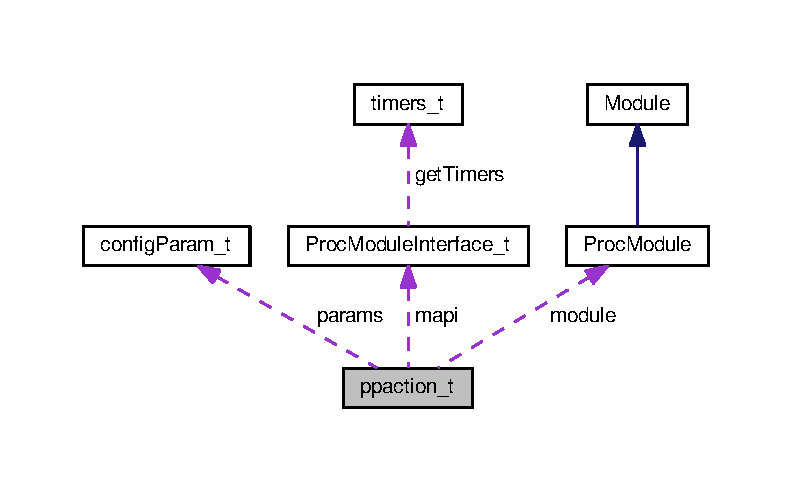
\includegraphics[width=350pt]{structppaction__t__coll__graph}
\end{center}
\end{figure}
\subsection*{Public Attributes}
\begin{DoxyCompactItemize}
\item 
\mbox{\Hypertarget{structppaction__t_aacb8715e6ca2050f983fca8852f0c789}\label{structppaction__t_aacb8715e6ca2050f983fca8852f0c789}} 
\hyperlink{classProcModule}{Proc\+Module} $\ast$ {\bfseries module}
\item 
\mbox{\Hypertarget{structppaction__t_a1538e65dcb9e5caa38817cf777e303b6}\label{structppaction__t_a1538e65dcb9e5caa38817cf777e303b6}} 
\hyperlink{structProcModuleInterface__t}{Proc\+Module\+Interface\+\_\+t} $\ast$ {\bfseries mapi}
\item 
\mbox{\Hypertarget{structppaction__t_ab277d78a7f33eea3935df8fd942693bc}\label{structppaction__t_ab277d78a7f33eea3935df8fd942693bc}} 
void $\ast$ {\bfseries flow\+Data}
\item 
\mbox{\Hypertarget{structppaction__t_af241587678add3ae9f2cea09f3468613}\label{structppaction__t_af241587678add3ae9f2cea09f3468613}} 
\hyperlink{structconfigParam__t}{config\+Param\+\_\+t} $\ast$ {\bfseries params}
\end{DoxyCompactItemize}


The documentation for this struct was generated from the following file\+:\begin{DoxyCompactItemize}
\item 
include/\hyperlink{QOSProcessor_8h}{Q\+O\+S\+Processor.\+h}\end{DoxyCompactItemize}

\hypertarget{structpprot}{}\section{pprot Struct Reference}
\label{structpprot}\index{pprot@{pprot}}
\subsection*{Public Attributes}
\begin{DoxyCompactItemize}
\item 
\mbox{\Hypertarget{structpprot_a83158e600d1d1e694818b1d1e5251896}\label{structpprot_a83158e600d1d1e694818b1d1e5251896}} 
const char $\ast$ {\bfseries name}
\item 
\mbox{\Hypertarget{structpprot_af0912e98c2c23259d2c7638f85be80d4}\label{structpprot_af0912e98c2c23259d2c7638f85be80d4}} 
u\+\_\+int8\+\_\+t {\bfseries num}
\end{DoxyCompactItemize}


The documentation for this struct was generated from the following file\+:\begin{DoxyCompactItemize}
\item 
proc\+\_\+modules/\hyperlink{htb_8cpp}{htb.\+cpp}\end{DoxyCompactItemize}

\hypertarget{classProcError}{}\section{Proc\+Error Class Reference}
\label{classProcError}\index{Proc\+Error@{Proc\+Error}}


generic error exception  




{\ttfamily \#include $<$Proc\+Error.\+h$>$}

\subsection*{Public Member Functions}
\begin{DoxyCompactItemize}
\item 
\hyperlink{classProcError_af2f56765e672178cba7f8105bd3347eb}{Proc\+Error} ()
\begin{DoxyCompactList}\small\item\em $<$ create unnamed error exception \end{DoxyCompactList}\item 
\mbox{\Hypertarget{classProcError_ab9d1e4acf156799d955b080ea6e19fe0}\label{classProcError_ab9d1e4acf156799d955b080ea6e19fe0}} 
\hyperlink{classProcError_ab9d1e4acf156799d955b080ea6e19fe0}{Proc\+Error} (const std\+::string new\+\_\+error=\char`\"{}\char`\"{})
\begin{DoxyCompactList}\small\item\em create named error exception \end{DoxyCompactList}\item 
\mbox{\Hypertarget{classProcError_af69e2425daf414e2ca77835e9849ba0f}\label{classProcError_af69e2425daf414e2ca77835e9849ba0f}} 
\hyperlink{classProcError_af69e2425daf414e2ca77835e9849ba0f}{Proc\+Error} (const int err\+\_\+no=0, const std\+::string err\+\_\+str=\char`\"{}\char`\"{})
\begin{DoxyCompactList}\small\item\em printf-\/style constructor \end{DoxyCompactList}\item 
\mbox{\Hypertarget{classProcError_a8c58217001468841f21a73473836b931}\label{classProcError_a8c58217001468841f21a73473836b931}} 
\hyperlink{classProcError_a8c58217001468841f21a73473836b931}{Proc\+Error} (const int err\+\_\+no, const char $\ast$fmt,...)
\begin{DoxyCompactList}\small\item\em printf-\/style constructor \end{DoxyCompactList}\item 
\mbox{\Hypertarget{classProcError_ade1a00fb8c459df2f1fd9d04db346092}\label{classProcError_ade1a00fb8c459df2f1fd9d04db346092}} 
\hyperlink{classProcError_ade1a00fb8c459df2f1fd9d04db346092}{Proc\+Error} (const char $\ast$fmt,...)
\begin{DoxyCompactList}\small\item\em get error msg from exception \end{DoxyCompactList}\item 
\mbox{\Hypertarget{classProcError_a3cd2078d3ab4794921b86e1b4cd69519}\label{classProcError_a3cd2078d3ab4794921b86e1b4cd69519}} 
std\+::string {\bfseries get\+Error} ()
\item 
\mbox{\Hypertarget{classProcError_a73c98b8bad445fcb90c6011e93edecb2}\label{classProcError_a73c98b8bad445fcb90c6011e93edecb2}} 
int \hyperlink{classProcError_a73c98b8bad445fcb90c6011e93edecb2}{get\+Error\+No} ()
\begin{DoxyCompactList}\small\item\em get error number \end{DoxyCompactList}\item 
\mbox{\Hypertarget{classProcError_a8415fe24bf03c639866cfc04a3dce64e}\label{classProcError_a8415fe24bf03c639866cfc04a3dce64e}} 
void {\bfseries dump} (std\+::ostream \&os)
\end{DoxyCompactItemize}
\subsection*{Protected Attributes}
\begin{DoxyCompactItemize}
\item 
int \hyperlink{classProcError_a0bd2a883852f733b07b6b896f5a51d0c}{error\+No}
\begin{DoxyCompactList}\small\item\em error number \end{DoxyCompactList}\item 
\mbox{\Hypertarget{classProcError_a35664f060a696d177230840b0b248080}\label{classProcError_a35664f060a696d177230840b0b248080}} 
std\+::string {\bfseries error}
\end{DoxyCompactItemize}


\subsection{Detailed Description}
generic error exception 

\hyperlink{classError}{Error} represents an exception that can be thrown. It includes a string that can be used to further specify the error encountered. Optionally it also includes a number. 

\subsection{Constructor \& Destructor Documentation}
\mbox{\Hypertarget{classProcError_af2f56765e672178cba7f8105bd3347eb}\label{classProcError_af2f56765e672178cba7f8105bd3347eb}} 
\index{Proc\+Error@{Proc\+Error}!Proc\+Error@{Proc\+Error}}
\index{Proc\+Error@{Proc\+Error}!Proc\+Error@{Proc\+Error}}
\subsubsection{\texorpdfstring{Proc\+Error()}{ProcError()}}
{\footnotesize\ttfamily Proc\+Error\+::\+Proc\+Error (\begin{DoxyParamCaption}{ }\end{DoxyParamCaption})\hspace{0.3cm}{\ttfamily [inline]}}



$<$ create unnamed error exception 

create named error exception 

\subsection{Member Data Documentation}
\mbox{\Hypertarget{classProcError_a0bd2a883852f733b07b6b896f5a51d0c}\label{classProcError_a0bd2a883852f733b07b6b896f5a51d0c}} 
\index{Proc\+Error@{Proc\+Error}!error\+No@{error\+No}}
\index{error\+No@{error\+No}!Proc\+Error@{Proc\+Error}}
\subsubsection{\texorpdfstring{error\+No}{errorNo}}
{\footnotesize\ttfamily int Proc\+Error\+::error\+No\hspace{0.3cm}{\ttfamily [protected]}}



error number 

error string 

The documentation for this class was generated from the following files\+:\begin{DoxyCompactItemize}
\item 
include/\hyperlink{ProcError_8h}{Proc\+Error.\+h}\item 
proc\+\_\+modules/\hyperlink{ProcError_8cpp}{Proc\+Error.\+cpp}\end{DoxyCompactItemize}

\hypertarget{classProcModule}{}\section{Proc\+Module Class Reference}
\label{classProcModule}\index{Proc\+Module@{Proc\+Module}}


container class that stores information about an evaluation module  




{\ttfamily \#include $<$Proc\+Module.\+h$>$}



Inheritance diagram for Proc\+Module\+:
\nopagebreak
\begin{figure}[H]
\begin{center}
\leavevmode
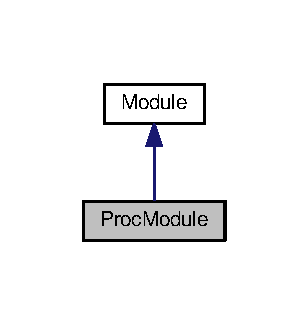
\includegraphics[width=148pt]{classProcModule__inherit__graph}
\end{center}
\end{figure}


Collaboration diagram for Proc\+Module\+:
\nopagebreak
\begin{figure}[H]
\begin{center}
\leavevmode
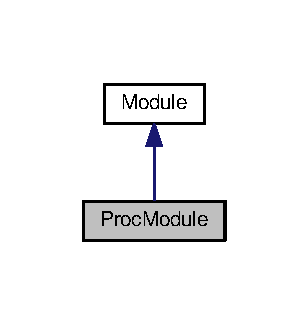
\includegraphics[width=148pt]{classProcModule__coll__graph}
\end{center}
\end{figure}
\subsection*{Public Member Functions}
\begin{DoxyCompactItemize}
\item 
\mbox{\Hypertarget{classProcModule_a780d31e8458d25ea9ba7004d044509dd}\label{classProcModule_a780d31e8458d25ea9ba7004d044509dd}} 
\hyperlink{structtypeInfo__t}{type\+Info\+\_\+t} $\ast$ {\bfseries get\+Type\+Info} ()
\item 
\mbox{\Hypertarget{classProcModule_a3bba66dde9395f27cc4f8982282e2b54}\label{classProcModule_a3bba66dde9395f27cc4f8982282e2b54}} 
\hyperlink{structProcModuleInterface__t}{Proc\+Module\+Interface\+\_\+t} $\ast$ {\bfseries get\+A\+PI} ()
\item 
\mbox{\Hypertarget{classProcModule_a7b53fc4aab791ebf29caf709720b95f2}\label{classProcModule_a7b53fc4aab791ebf29caf709720b95f2}} 
virtual string {\bfseries get\+Module\+Type} ()
\item 
\mbox{\Hypertarget{classProcModule_aedb442504493c7d4b910ba7cc4a9c346}\label{classProcModule_aedb442504493c7d4b910ba7cc4a9c346}} 
virtual int {\bfseries get\+Version} ()
\item 
\mbox{\Hypertarget{classProcModule_aef74018a555606e63d4703fc7be4b1af}\label{classProcModule_aef74018a555606e63d4703fc7be4b1af}} 
const char $\ast$ {\bfseries get\+Module\+Info} (int i)
\item 
\hyperlink{classProcModule_a3dcb3d64eae9628446986b254073cb4f}{Proc\+Module} (\hyperlink{classConfigManager}{Config\+Manager} $\ast$\+\_\+cnf, string libname, string libfile, \hyperlink{Module_8h_acbeb44869400b78e5f4097d5c49fc093}{lib\+Handle\+\_\+t} libhandle, string confgroup)
\begin{DoxyCompactList}\small\item\em construct and initialize a \hyperlink{classProcModule}{Proc\+Module} object \end{DoxyCompactList}\item 
\mbox{\Hypertarget{classProcModule_a8f2ee6251014ab5b53e81f8f40db0205}\label{classProcModule_a8f2ee6251014ab5b53e81f8f40db0205}} 
\hyperlink{classProcModule_a8f2ee6251014ab5b53e81f8f40db0205}{$\sim$\+Proc\+Module} ()
\begin{DoxyCompactList}\small\item\em destroy a \hyperlink{classProcModule}{Proc\+Module} object \end{DoxyCompactList}\item 
\mbox{\Hypertarget{classProcModule_ad0559892993237ae19152400da9216e6}\label{classProcModule_ad0559892993237ae19152400da9216e6}} 
string \hyperlink{classProcModule_ad0559892993237ae19152400da9216e6}{make\+Module\+Info\+X\+ML} ()
\begin{DoxyCompactList}\small\item\em generate textual module description in X\+ML format from text data stored in module itself, writes module\+Info\+X\+ML \end{DoxyCompactList}\item 
\mbox{\Hypertarget{classProcModule_a7274ea6967f8a29e74b3f15460d2f7d7}\label{classProcModule_a7274ea6967f8a29e74b3f15460d2f7d7}} 
string \hyperlink{classProcModule_a7274ea6967f8a29e74b3f15460d2f7d7}{get\+Module\+Info\+X\+ML} ()
\begin{DoxyCompactList}\small\item\em return textual module description in X\+ML format \end{DoxyCompactList}\item 
\mbox{\Hypertarget{classProcModule_a3be2709976cf53033187b6dcf8c773ef}\label{classProcModule_a3be2709976cf53033187b6dcf8c773ef}} 
string \hyperlink{classProcModule_a3be2709976cf53033187b6dcf8c773ef}{get\+Type\+Info\+Text} ()
\begin{DoxyCompactList}\small\item\em return a textual representation of this modules export info structure \end{DoxyCompactList}\item 
\mbox{\Hypertarget{classProcModule_af465814c2e6d29c1a0b5d0612766a3b6}\label{classProcModule_af465814c2e6d29c1a0b5d0612766a3b6}} 
void \hyperlink{classProcModule_af465814c2e6d29c1a0b5d0612766a3b6}{dump} (ostream \&os)
\begin{DoxyCompactList}\small\item\em dump a \hyperlink{classProcModule}{Proc\+Module} object \end{DoxyCompactList}\end{DoxyCompactItemize}
\subsection*{Static Public Member Functions}
\begin{DoxyCompactItemize}
\item 
\mbox{\Hypertarget{classProcModule_a9403c5e74c333c1885087dc577d07e22}\label{classProcModule_a9403c5e74c333c1885087dc577d07e22}} 
static string \hyperlink{classProcModule_a9403c5e74c333c1885087dc577d07e22}{info\+Label} (int i)
\begin{DoxyCompactList}\small\item\em get text label for type property i \end{DoxyCompactList}\item 
\mbox{\Hypertarget{classProcModule_a8e1f0c83dbe077e57d3b9990ee3308db}\label{classProcModule_a8e1f0c83dbe077e57d3b9990ee3308db}} 
static string \hyperlink{classProcModule_a8e1f0c83dbe077e57d3b9990ee3308db}{type\+Label} (int i)
\begin{DoxyCompactList}\small\item\em get text label for type property i \end{DoxyCompactList}\end{DoxyCompactItemize}


\subsection{Detailed Description}
container class that stores information about an evaluation module 

container class -\/ stores information about an evaluation module such as name, uid, function list, libhandle and reference counter 

\subsection{Constructor \& Destructor Documentation}
\mbox{\Hypertarget{classProcModule_a3dcb3d64eae9628446986b254073cb4f}\label{classProcModule_a3dcb3d64eae9628446986b254073cb4f}} 
\index{Proc\+Module@{Proc\+Module}!Proc\+Module@{Proc\+Module}}
\index{Proc\+Module@{Proc\+Module}!Proc\+Module@{Proc\+Module}}
\subsubsection{\texorpdfstring{Proc\+Module()}{ProcModule()}}
{\footnotesize\ttfamily Proc\+Module\+::\+Proc\+Module (\begin{DoxyParamCaption}\item[{\hyperlink{classConfigManager}{Config\+Manager} $\ast$}]{\+\_\+cnf,  }\item[{string}]{libname,  }\item[{string}]{libfile,  }\item[{\hyperlink{Module_8h_acbeb44869400b78e5f4097d5c49fc093}{lib\+Handle\+\_\+t}}]{libhandle,  }\item[{string}]{confgroup }\end{DoxyParamCaption})}



construct and initialize a \hyperlink{classProcModule}{Proc\+Module} object 

take the library handle of an evaluation module and retrieve all the other information (name, uid, function list) via this handle

\begin{DoxyItemize}
\item {\ttfamily \+\_\+cnf} -\/ link to configuration manager (for cfg file query) \item {\ttfamily libname} -\/ name of the evaluation module \item {\ttfamily filename} -\/ name of module including path and extension \item {\ttfamily libhandle} -\/ system handle for loaded library (see dlopen) \item {\ttfamily confgroup} -\/ Configuration group for the module. \end{DoxyItemize}


The documentation for this class was generated from the following files\+:\begin{DoxyCompactItemize}
\item 
include/Proc\+Module.\+h\item 
src/Proc\+Module.\+cpp\end{DoxyCompactItemize}

\hypertarget{structProcModuleInterface__t}{}\section{Proc\+Module\+Interface\+\_\+t Struct Reference}
\label{structProcModuleInterface__t}\index{Proc\+Module\+Interface\+\_\+t@{Proc\+Module\+Interface\+\_\+t}}


definition of interface struct for Action Modules  




{\ttfamily \#include $<$Proc\+Module\+Interface.\+h$>$}



Collaboration diagram for Proc\+Module\+Interface\+\_\+t\+:
\nopagebreak
\begin{figure}[H]
\begin{center}
\leavevmode
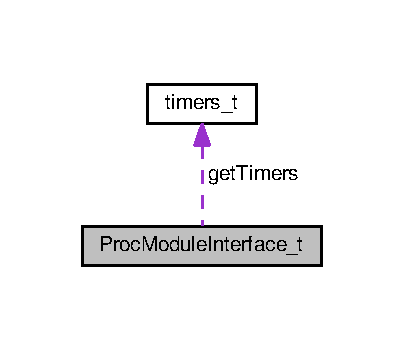
\includegraphics[width=194pt]{structProcModuleInterface__t__coll__graph}
\end{center}
\end{figure}
\subsection*{Public Attributes}
\begin{DoxyCompactItemize}
\item 
\mbox{\Hypertarget{structProcModuleInterface__t_acfd41eed5bbd3b6dd40cb9f4c3200259}\label{structProcModuleInterface__t_acfd41eed5bbd3b6dd40cb9f4c3200259}} 
int {\bfseries version}
\item 
\mbox{\Hypertarget{structProcModuleInterface__t_a52d61a61e5f9bc99302ad4391dd63320}\label{structProcModuleInterface__t_a52d61a61e5f9bc99302ad4391dd63320}} 
void($\ast$ {\bfseries init\+Module} )(\hyperlink{structconfigParam__t}{config\+Param\+\_\+t} $\ast$params)
\item 
\mbox{\Hypertarget{structProcModuleInterface__t_a7e1fdbeabf56530af6704a3781470b77}\label{structProcModuleInterface__t_a7e1fdbeabf56530af6704a3781470b77}} 
void($\ast$ {\bfseries destroy\+Module} )(\hyperlink{structconfigParam__t}{config\+Param\+\_\+t} $\ast$params)
\item 
\mbox{\Hypertarget{structProcModuleInterface__t_a4cb210433fd498ddffff3514d801aeb7}\label{structProcModuleInterface__t_a4cb210433fd498ddffff3514d801aeb7}} 
void($\ast$ {\bfseries init\+Flow\+Setup} )(\hyperlink{structconfigParam__t}{config\+Param\+\_\+t} $\ast$params, \hyperlink{ProcModuleInterface_8h_a2afc1e9fc63b2cfcd86ec2435f24e27c}{filter\+List\+\_\+t} $\ast$filters, void $\ast$$\ast$flowdata)
\item 
\mbox{\Hypertarget{structProcModuleInterface__t_a938795aaa627bce229f93ee3c245ea4c}\label{structProcModuleInterface__t_a938795aaa627bce229f93ee3c245ea4c}} 
\hyperlink{structtimers__t}{timers\+\_\+t} $\ast$($\ast$ {\bfseries get\+Timers} )(void $\ast$flowdata)
\item 
\mbox{\Hypertarget{structProcModuleInterface__t_a4b64d61793632aa822155f5bc0a44c3b}\label{structProcModuleInterface__t_a4b64d61793632aa822155f5bc0a44c3b}} 
void($\ast$ {\bfseries destroy\+Flow\+Setup} )(\hyperlink{structconfigParam__t}{config\+Param\+\_\+t} $\ast$params, \hyperlink{ProcModuleInterface_8h_a2afc1e9fc63b2cfcd86ec2435f24e27c}{filter\+List\+\_\+t} $\ast$filters, void $\ast$flowdata)
\item 
\mbox{\Hypertarget{structProcModuleInterface__t_afa248e185040d67ea5fd189c39ab02bf}\label{structProcModuleInterface__t_afa248e185040d67ea5fd189c39ab02bf}} 
void($\ast$ {\bfseries reset\+Flow\+Setup} )(\hyperlink{structconfigParam__t}{config\+Param\+\_\+t} $\ast$params)
\item 
\mbox{\Hypertarget{structProcModuleInterface__t_a011a7f17fb169d26bf1c4224d967c7b3}\label{structProcModuleInterface__t_a011a7f17fb169d26bf1c4224d967c7b3}} 
int($\ast$ {\bfseries check\+Band\+Width} )(\hyperlink{structconfigParam__t}{config\+Param\+\_\+t} $\ast$params)
\item 
\mbox{\Hypertarget{structProcModuleInterface__t_a891358873cd1264013a61a136e705a82}\label{structProcModuleInterface__t_a891358873cd1264013a61a136e705a82}} 
void($\ast$ {\bfseries timeout} )(int timer\+ID, void $\ast$flowdata)
\item 
\mbox{\Hypertarget{structProcModuleInterface__t_a924c70b60eef375c72dffad4e5f33671}\label{structProcModuleInterface__t_a924c70b60eef375c72dffad4e5f33671}} 
const char $\ast$($\ast$ {\bfseries get\+Module\+Info} )(int i)
\item 
\mbox{\Hypertarget{structProcModuleInterface__t_a0e045475982315a86919a0fe98e9eab2}\label{structProcModuleInterface__t_a0e045475982315a86919a0fe98e9eab2}} 
char $\ast$($\ast$ {\bfseries get\+Error\+Msg} )(int code)
\end{DoxyCompactItemize}


\subsection{Detailed Description}
definition of interface struct for Action Modules 

this structure contains pointers to all functions of this module which are part of the Action \hyperlink{classModule}{Module} A\+PI. It will be automatically set for an Action \hyperlink{classModule}{Module} upon compilation (don\textquotesingle{}t forget to include Action\+Module.\+h into every module!) 

The documentation for this struct was generated from the following file\+:\begin{DoxyCompactItemize}
\item 
include/\hyperlink{ProcModuleInterface_8h}{Proc\+Module\+Interface.\+h}\end{DoxyCompactItemize}

\hypertarget{classProcTimerEvent}{}\section{Proc\+Timer\+Event Class Reference}
\label{classProcTimerEvent}\index{Proc\+Timer\+Event@{Proc\+Timer\+Event}}


Inheritance diagram for Proc\+Timer\+Event\+:
\nopagebreak
\begin{figure}[H]
\begin{center}
\leavevmode
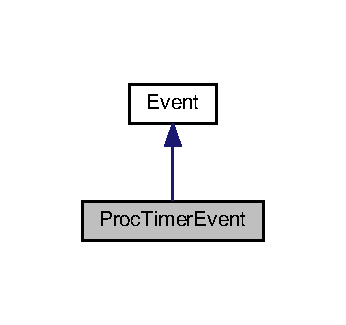
\includegraphics[width=166pt]{classProcTimerEvent__inherit__graph}
\end{center}
\end{figure}


Collaboration diagram for Proc\+Timer\+Event\+:
\nopagebreak
\begin{figure}[H]
\begin{center}
\leavevmode
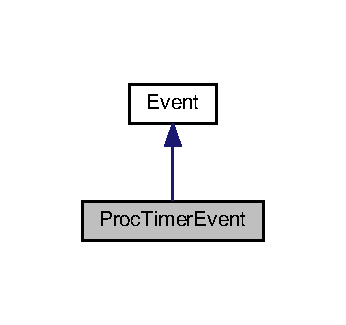
\includegraphics[width=166pt]{classProcTimerEvent__coll__graph}
\end{center}
\end{figure}
\subsection*{Public Member Functions}
\begin{DoxyCompactItemize}
\item 
\mbox{\Hypertarget{classProcTimerEvent_ae81e8a0e9d4913cf10efe6908434952b}\label{classProcTimerEvent_ae81e8a0e9d4913cf10efe6908434952b}} 
{\bfseries Proc\+Timer\+Event} (int rule\+ID, int act\+ID, \hyperlink{structtimers__t}{timers\+\_\+t} $\ast$timer)
\item 
\mbox{\Hypertarget{classProcTimerEvent_a4b46028129b4d933c38c2ffd7d6e1b87}\label{classProcTimerEvent_a4b46028129b4d933c38c2ffd7d6e1b87}} 
int {\bfseries get\+R\+ID} ()
\item 
\mbox{\Hypertarget{classProcTimerEvent_aaba1899c5a1bd53028863262a6d39424}\label{classProcTimerEvent_aaba1899c5a1bd53028863262a6d39424}} 
int {\bfseries get\+A\+ID} ()
\item 
\mbox{\Hypertarget{classProcTimerEvent_ab40244b1fdd5f47487f171eecd49c2b3}\label{classProcTimerEvent_ab40244b1fdd5f47487f171eecd49c2b3}} 
unsigned int {\bfseries get\+T\+ID} ()
\item 
\mbox{\Hypertarget{classProcTimerEvent_aaf40ef6f4e15ff672b004d3856eef860}\label{classProcTimerEvent_aaf40ef6f4e15ff672b004d3856eef860}} 
int \hyperlink{classProcTimerEvent_aaf40ef6f4e15ff672b004d3856eef860}{delete\+Rule} (int uid)
\begin{DoxyCompactList}\small\item\em delete rules stored in this event \end{DoxyCompactList}\end{DoxyCompactItemize}
\subsection*{Public Attributes}
\begin{DoxyCompactItemize}
\item 
\mbox{\Hypertarget{classProcTimerEvent_aeeedb2fd2c111aba58f733a727cf4e19}\label{classProcTimerEvent_aeeedb2fd2c111aba58f733a727cf4e19}} 
int {\bfseries rid}
\item 
\mbox{\Hypertarget{classProcTimerEvent_a42590019ad4036654c14f04758658c16}\label{classProcTimerEvent_a42590019ad4036654c14f04758658c16}} 
int {\bfseries actid}
\item 
\mbox{\Hypertarget{classProcTimerEvent_ab71572f4955b2851cf4fa12ccd84c5d3}\label{classProcTimerEvent_ab71572f4955b2851cf4fa12ccd84c5d3}} 
unsigned int {\bfseries tm\+ID}
\end{DoxyCompactItemize}


The documentation for this class was generated from the following file\+:\begin{DoxyCompactItemize}
\item 
include/\hyperlink{Event_8h}{Event.\+h}\end{DoxyCompactItemize}

\hypertarget{classQOSProcessor}{}\section{Q\+O\+S\+Processor Class Reference}
\label{classQOSProcessor}\index{Q\+O\+S\+Processor@{Q\+O\+S\+Processor}}


manage and apply Action Modules, retrieve flow data  




{\ttfamily \#include $<$Q\+O\+S\+Processor.\+h$>$}



Inheritance diagram for Q\+O\+S\+Processor\+:
\nopagebreak
\begin{figure}[H]
\begin{center}
\leavevmode
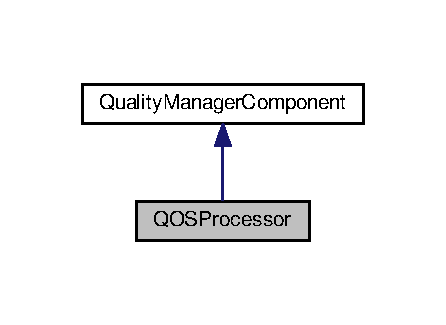
\includegraphics[width=214pt]{classQOSProcessor__inherit__graph}
\end{center}
\end{figure}


Collaboration diagram for Q\+O\+S\+Processor\+:
\nopagebreak
\begin{figure}[H]
\begin{center}
\leavevmode
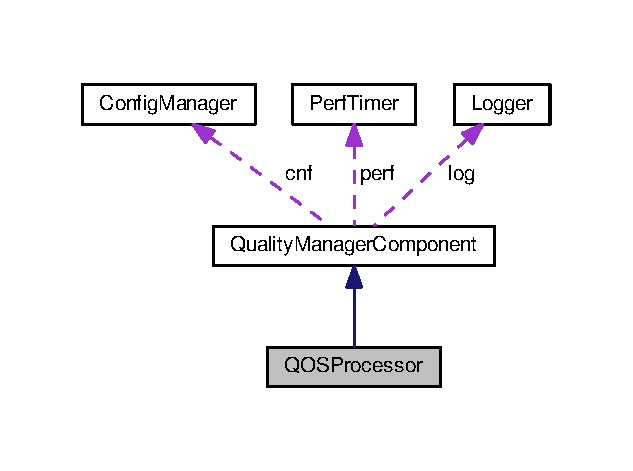
\includegraphics[width=304pt]{classQOSProcessor__coll__graph}
\end{center}
\end{figure}
\subsection*{Public Member Functions}
\begin{DoxyCompactItemize}
\item 
\hyperlink{classQOSProcessor_a27b56d900e42f99fea52c93e8a720bf5}{Q\+O\+S\+Processor} (\hyperlink{classConfigManager}{Config\+Manager} $\ast$\hyperlink{classQualityManagerComponent_a021f9991b72d52f295b87d8a5b02046a}{cnf}, int \hyperlink{classQualityManagerComponent_add2cffa903c310563f8b999cdecd1953}{threaded}, string module\+Dir=\char`\"{}\char`\"{})
\begin{DoxyCompactList}\small\item\em construct and initialize a Packet\+Processor object \end{DoxyCompactList}\item 
\mbox{\Hypertarget{classQOSProcessor_a78d0a0c0dde203f9deb4120feae114c3}\label{classQOSProcessor_a78d0a0c0dde203f9deb4120feae114c3}} 
virtual \hyperlink{classQOSProcessor_a78d0a0c0dde203f9deb4120feae114c3}{$\sim$\+Q\+O\+S\+Processor} ()
\begin{DoxyCompactList}\small\item\em destroy a Packet\+Processor object, to be overloaded \end{DoxyCompactList}\item 
\mbox{\Hypertarget{classQOSProcessor_ab9b3ef050bdc595e6096baac0d466955}\label{classQOSProcessor_ab9b3ef050bdc595e6096baac0d466955}} 
virtual void \hyperlink{classQOSProcessor_ab9b3ef050bdc595e6096baac0d466955}{check\+Rules} (\hyperlink{RuleFileParser_8h_a7d5bb94bb17a8a1d92db2a89a0cc96d1}{rule\+D\+B\+\_\+t} $\ast$rules)
\begin{DoxyCompactList}\small\item\em check a ruleset (the action part) \end{DoxyCompactList}\item 
\mbox{\Hypertarget{classQOSProcessor_a6370d2653a88ce6dc4df275b8279605e}\label{classQOSProcessor_a6370d2653a88ce6dc4df275b8279605e}} 
virtual void \hyperlink{classQOSProcessor_a6370d2653a88ce6dc4df275b8279605e}{add\+Rules} (\hyperlink{RuleFileParser_8h_a7d5bb94bb17a8a1d92db2a89a0cc96d1}{rule\+D\+B\+\_\+t} $\ast$rules, \hyperlink{classEventScheduler}{Event\+Scheduler} $\ast$e)
\begin{DoxyCompactList}\small\item\em add rules \end{DoxyCompactList}\item 
\mbox{\Hypertarget{classQOSProcessor_ab873474a8a86af31723c1a9c7bcd6efb}\label{classQOSProcessor_ab873474a8a86af31723c1a9c7bcd6efb}} 
virtual void \hyperlink{classQOSProcessor_ab873474a8a86af31723c1a9c7bcd6efb}{del\+Rules} (\hyperlink{RuleFileParser_8h_a7d5bb94bb17a8a1d92db2a89a0cc96d1}{rule\+D\+B\+\_\+t} $\ast$rules)
\begin{DoxyCompactList}\small\item\em delete rules \end{DoxyCompactList}\item 
\mbox{\Hypertarget{classQOSProcessor_ab929839bf92971682861fb8784f177c9}\label{classQOSProcessor_ab929839bf92971682861fb8784f177c9}} 
int \hyperlink{classQOSProcessor_ab929839bf92971682861fb8784f177c9}{check\+Rule} (\hyperlink{classRule}{Rule} $\ast$r)
\begin{DoxyCompactList}\small\item\em check a single rule \end{DoxyCompactList}\item 
int \hyperlink{classQOSProcessor_a6378d7fdd049553ad9a449d5c206c865}{add\+Rule} (\hyperlink{classRule}{Rule} $\ast$r, \hyperlink{classEventScheduler}{Event\+Scheduler} $\ast$e)
\begin{DoxyCompactList}\small\item\em add a \hyperlink{classRule}{Rule} and its associated actions to rule list \end{DoxyCompactList}\item 
int \hyperlink{classQOSProcessor_a4b287dd7fd9b024b841649a929fe80de}{del\+Rule} (\hyperlink{classRule}{Rule} $\ast$r)
\begin{DoxyCompactList}\small\item\em delete a \hyperlink{classRule}{Rule} from the rule list \end{DoxyCompactList}\item 
\mbox{\Hypertarget{classQOSProcessor_a96048b3439c2200ed3766cd009c41ed5}\label{classQOSProcessor_a96048b3439c2200ed3766cd009c41ed5}} 
virtual int \hyperlink{classQOSProcessor_a96048b3439c2200ed3766cd009c41ed5}{handle\+F\+D\+Event} (\hyperlink{QualityManagerComponent_8h_acd67c59a21d5c694ab882c8905db0a2a}{event\+Vec\+\_\+t} $\ast$e, fd\+\_\+set $\ast$rset, fd\+\_\+set $\ast$wset, \hyperlink{structfd__sets__t}{fd\+\_\+sets\+\_\+t} $\ast$fds)
\begin{DoxyCompactList}\small\item\em handle file descriptor event \end{DoxyCompactList}\item 
\mbox{\Hypertarget{classQOSProcessor_aa8c0438112f94a3ac43a67897dc5031b}\label{classQOSProcessor_aa8c0438112f94a3ac43a67897dc5031b}} 
void \hyperlink{classQOSProcessor_aa8c0438112f94a3ac43a67897dc5031b}{main} ()
\begin{DoxyCompactList}\small\item\em thread main function \end{DoxyCompactList}\item 
unsigned long \hyperlink{classQOSProcessor_a5c5fe6cac6644de9a8ef1f767ceab078}{rule\+Timeout} (int rule\+ID, unsigned long ival, time\+\_\+t now)
\begin{DoxyCompactList}\small\item\em return -\/1 (no packet seen), 0 (timeout), $>$0 (no timeout; adjust last time) \end{DoxyCompactList}\item 
\mbox{\Hypertarget{classQOSProcessor_a28dc4f55ef2a7f9ce115e89cbc961725}\label{classQOSProcessor_a28dc4f55ef2a7f9ce115e89cbc961725}} 
string \hyperlink{classQOSProcessor_a28dc4f55ef2a7f9ce115e89cbc961725}{get\+Info} ()
\begin{DoxyCompactList}\small\item\em get information about loaded modules \end{DoxyCompactList}\item 
\mbox{\Hypertarget{classQOSProcessor_a8b82498d97f1c971442fa91554916aa8}\label{classQOSProcessor_a8b82498d97f1c971442fa91554916aa8}} 
void \hyperlink{classQOSProcessor_a8b82498d97f1c971442fa91554916aa8}{dump} (ostream \&os)
\begin{DoxyCompactList}\small\item\em dump a Packet\+Processor object \end{DoxyCompactList}\item 
\mbox{\Hypertarget{classQOSProcessor_a75d32434a5b264d1d25e1d4e047bfbcc}\label{classQOSProcessor_a75d32434a5b264d1d25e1d4e047bfbcc}} 
int \hyperlink{classQOSProcessor_a75d32434a5b264d1d25e1d4e047bfbcc}{num\+Modules} ()
\begin{DoxyCompactList}\small\item\em get the number of action modules currently in use \end{DoxyCompactList}\item 
\mbox{\Hypertarget{classQOSProcessor_ac40c582964aa24aa2bc4feb028eaa2b0}\label{classQOSProcessor_ac40c582964aa24aa2bc4feb028eaa2b0}} 
void {\bfseries timeout} (int rid, int actid, unsigned int tm\+ID)
\item 
\mbox{\Hypertarget{classQOSProcessor_ad294917f7d2690fd755067bf36104cac}\label{classQOSProcessor_ad294917f7d2690fd755067bf36104cac}} 
string \hyperlink{classQOSProcessor_ad294917f7d2690fd755067bf36104cac}{get\+Module\+Info\+X\+ML} (string modname)
\begin{DoxyCompactList}\small\item\em get xml info for a specific module \end{DoxyCompactList}\item 
\mbox{\Hypertarget{classQOSProcessor_a8c7e40e85fa1b02b61a6218281ccb736}\label{classQOSProcessor_a8c7e40e85fa1b02b61a6218281ccb736}} 
virtual string \hyperlink{classQOSProcessor_a8c7e40e85fa1b02b61a6218281ccb736}{get\+Config\+Group} ()
\begin{DoxyCompactList}\small\item\em return the config group of the component \end{DoxyCompactList}\item 
\mbox{\Hypertarget{classQOSProcessor_afdc5230a402875b43ed3633621b151e2}\label{classQOSProcessor_afdc5230a402875b43ed3633621b151e2}} 
virtual void {\bfseries wait\+Until\+Done} ()
\end{DoxyCompactItemize}
\subsection*{Additional Inherited Members}


\subsection{Detailed Description}
manage and apply Action Modules, retrieve flow data 

the Packet\+Processor class allows to manage filter rules and their associated actions and apply those actions to incoming packets, manage and retrieve flow data 

\subsection{Constructor \& Destructor Documentation}
\mbox{\Hypertarget{classQOSProcessor_a27b56d900e42f99fea52c93e8a720bf5}\label{classQOSProcessor_a27b56d900e42f99fea52c93e8a720bf5}} 
\index{Q\+O\+S\+Processor@{Q\+O\+S\+Processor}!Q\+O\+S\+Processor@{Q\+O\+S\+Processor}}
\index{Q\+O\+S\+Processor@{Q\+O\+S\+Processor}!Q\+O\+S\+Processor@{Q\+O\+S\+Processor}}
\subsubsection{\texorpdfstring{Q\+O\+S\+Processor()}{QOSProcessor()}}
{\footnotesize\ttfamily Q\+O\+S\+Processor\+::\+Q\+O\+S\+Processor (\begin{DoxyParamCaption}\item[{\hyperlink{classConfigManager}{Config\+Manager} $\ast$}]{cnf,  }\item[{int}]{threaded,  }\item[{string}]{module\+Dir = {\ttfamily \char`\"{}\char`\"{}} }\end{DoxyParamCaption})}



construct and initialize a Packet\+Processor object 

\begin{DoxyItemize}
\item {\ttfamily cnf} config manager \item {\ttfamily threaded} run as separate thread \item {\ttfamily module\+Dir} action module directory \end{DoxyItemize}


\subsection{Member Function Documentation}
\mbox{\Hypertarget{classQOSProcessor_a6378d7fdd049553ad9a449d5c206c865}\label{classQOSProcessor_a6378d7fdd049553ad9a449d5c206c865}} 
\index{Q\+O\+S\+Processor@{Q\+O\+S\+Processor}!add\+Rule@{add\+Rule}}
\index{add\+Rule@{add\+Rule}!Q\+O\+S\+Processor@{Q\+O\+S\+Processor}}
\subsubsection{\texorpdfstring{add\+Rule()}{addRule()}}
{\footnotesize\ttfamily int Q\+O\+S\+Processor\+::add\+Rule (\begin{DoxyParamCaption}\item[{\hyperlink{classRule}{Rule} $\ast$}]{r,  }\item[{\hyperlink{classEventScheduler}{Event\+Scheduler} $\ast$}]{e }\end{DoxyParamCaption})}



add a \hyperlink{classRule}{Rule} and its associated actions to rule list 

\begin{DoxyItemize}
\item {\ttfamily r} pointer to rule \item {\ttfamily e} pointer to event scheduler (timer events) \begin{DoxyReturn}{Returns}
0 -\/ on success, $<$0 -\/ else 
\end{DoxyReturn}
\end{DoxyItemize}
\mbox{\Hypertarget{classQOSProcessor_a4b287dd7fd9b024b841649a929fe80de}\label{classQOSProcessor_a4b287dd7fd9b024b841649a929fe80de}} 
\index{Q\+O\+S\+Processor@{Q\+O\+S\+Processor}!del\+Rule@{del\+Rule}}
\index{del\+Rule@{del\+Rule}!Q\+O\+S\+Processor@{Q\+O\+S\+Processor}}
\subsubsection{\texorpdfstring{del\+Rule()}{delRule()}}
{\footnotesize\ttfamily int Q\+O\+S\+Processor\+::del\+Rule (\begin{DoxyParamCaption}\item[{\hyperlink{classRule}{Rule} $\ast$}]{r }\end{DoxyParamCaption})}



delete a \hyperlink{classRule}{Rule} from the rule list 

\begin{DoxyItemize}
\item {\ttfamily r} pointer to rule \begin{DoxyReturn}{Returns}
0 -\/ on success, $<$0 -\/ else 
\end{DoxyReturn}
\end{DoxyItemize}
\mbox{\Hypertarget{classQOSProcessor_a5c5fe6cac6644de9a8ef1f767ceab078}\label{classQOSProcessor_a5c5fe6cac6644de9a8ef1f767ceab078}} 
\index{Q\+O\+S\+Processor@{Q\+O\+S\+Processor}!rule\+Timeout@{rule\+Timeout}}
\index{rule\+Timeout@{rule\+Timeout}!Q\+O\+S\+Processor@{Q\+O\+S\+Processor}}
\subsubsection{\texorpdfstring{rule\+Timeout()}{ruleTimeout()}}
{\footnotesize\ttfamily unsigned long Q\+O\+S\+Processor\+::rule\+Timeout (\begin{DoxyParamCaption}\item[{int}]{rule\+ID,  }\item[{unsigned long}]{ival,  }\item[{time\+\_\+t}]{now }\end{DoxyParamCaption})}



return -\/1 (no packet seen), 0 (timeout), $>$0 (no timeout; adjust last time) 

\begin{DoxyItemize}
\item {\ttfamily rule\+Id} -\/ number indicating matching rule for packet \end{DoxyItemize}


The documentation for this class was generated from the following files\+:\begin{DoxyCompactItemize}
\item 
include/\hyperlink{QOSProcessor_8h}{Q\+O\+S\+Processor.\+h}\item 
src/\hyperlink{QOSProcessor_8cpp}{Q\+O\+S\+Processor.\+cpp}\end{DoxyCompactItemize}

\hypertarget{classQualityManager}{}\section{Quality\+Manager Class Reference}
\label{classQualityManager}\index{Quality\+Manager@{Quality\+Manager}}


Quality Manager class description.  




{\ttfamily \#include $<$Quality\+Manager.\+h$>$}

\subsection*{Public Member Functions}
\begin{DoxyCompactItemize}
\item 
\hyperlink{classQualityManager_a0ac2ca4170c2b202b06501dc1be517ee}{Quality\+Manager} (int argc, char $\ast$argv\mbox{[}$\,$\mbox{]})
\begin{DoxyCompactList}\small\item\em construct and initialize a Quality Manager object \end{DoxyCompactList}\item 
\mbox{\Hypertarget{classQualityManager_a5002f1818e38a04f58a0419eb3eda29e}\label{classQualityManager_a5002f1818e38a04f58a0419eb3eda29e}} 
\hyperlink{classQualityManager_a5002f1818e38a04f58a0419eb3eda29e}{$\sim$\+Quality\+Manager} ()
\begin{DoxyCompactList}\small\item\em destroy a Quality Manager object detailed destructor description for Quality Manager \end{DoxyCompactList}\item 
\mbox{\Hypertarget{classQualityManager_ae822d80c4e5108e3a92cadccd16ae7f4}\label{classQualityManager_ae822d80c4e5108e3a92cadccd16ae7f4}} 
void {\bfseries run} ()
\item 
\mbox{\Hypertarget{classQualityManager_a8f8fb9e821500a0669faff26057d4abd}\label{classQualityManager_a8f8fb9e821500a0669faff26057d4abd}} 
void \hyperlink{classQualityManager_a8f8fb9e821500a0669faff26057d4abd}{dump} (ostream \&os)
\begin{DoxyCompactList}\small\item\em dump a Quality Manager object \end{DoxyCompactList}\item 
\mbox{\Hypertarget{classQualityManager_a47b33c808619f174d50059d99ac1a748}\label{classQualityManager_a47b33c808619f174d50059d99ac1a748}} 
void \hyperlink{classQualityManager_a47b33c808619f174d50059d99ac1a748}{handle\+Event} (\hyperlink{classEvent}{Event} $\ast$e, \hyperlink{structfd__sets__t}{fd\+\_\+sets\+\_\+t} $\ast$fds)
\begin{DoxyCompactList}\small\item\em handle the events \end{DoxyCompactList}\end{DoxyCompactItemize}
\subsection*{Static Public Attributes}
\begin{DoxyCompactItemize}
\item 
\mbox{\Hypertarget{classQualityManager_abf272ec740cc8baa0befd02755c49bce}\label{classQualityManager_abf272ec740cc8baa0befd02755c49bce}} 
static int {\bfseries s\+\_\+sigpipe} \mbox{[}2\mbox{]}
\end{DoxyCompactItemize}


\subsection{Detailed Description}
Quality Manager class description. 

detailed Quality Manager class description 

\subsection{Constructor \& Destructor Documentation}
\mbox{\Hypertarget{classQualityManager_a0ac2ca4170c2b202b06501dc1be517ee}\label{classQualityManager_a0ac2ca4170c2b202b06501dc1be517ee}} 
\index{Quality\+Manager@{Quality\+Manager}!Quality\+Manager@{Quality\+Manager}}
\index{Quality\+Manager@{Quality\+Manager}!Quality\+Manager@{Quality\+Manager}}
\subsubsection{\texorpdfstring{Quality\+Manager()}{QualityManager()}}
{\footnotesize\ttfamily Quality\+Manager\+::\+Quality\+Manager (\begin{DoxyParamCaption}\item[{int}]{argc,  }\item[{char $\ast$}]{argv\mbox{[}$\,$\mbox{]} }\end{DoxyParamCaption})}



construct and initialize a Quality Manager object 

detailed constructor description for Meter

\begin{DoxyItemize}
\item {\ttfamily argc} -\/ number of command line arguments \item {\ttfamily argv} -\/ list of command line arguments \end{DoxyItemize}


The documentation for this class was generated from the following files\+:\begin{DoxyCompactItemize}
\item 
include/\hyperlink{QualityManager_8h}{Quality\+Manager.\+h}\item 
src/\hyperlink{QualityManager_8cpp}{Quality\+Manager.\+cpp}\end{DoxyCompactItemize}

\hypertarget{classQualityManagerComponent}{}\section{Quality\+Manager\+Component Class Reference}
\label{classQualityManagerComponent}\index{Quality\+Manager\+Component@{Quality\+Manager\+Component}}


{\ttfamily \#include $<$Quality\+Manager\+Component.\+h$>$}



Inheritance diagram for Quality\+Manager\+Component\+:
\nopagebreak
\begin{figure}[H]
\begin{center}
\leavevmode
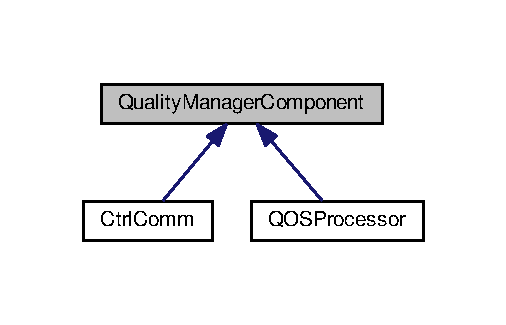
\includegraphics[width=243pt]{classQualityManagerComponent__inherit__graph}
\end{center}
\end{figure}


Collaboration diagram for Quality\+Manager\+Component\+:
\nopagebreak
\begin{figure}[H]
\begin{center}
\leavevmode
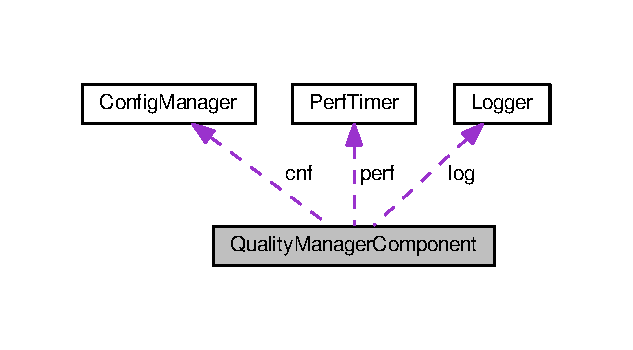
\includegraphics[width=304pt]{classQualityManagerComponent__coll__graph}
\end{center}
\end{figure}
\subsection*{Public Member Functions}
\begin{DoxyCompactItemize}
\item 
\hyperlink{classQualityManagerComponent_aa4185d8564d0ef37f12e2564a49aa727}{Quality\+Manager\+Component} (\hyperlink{classConfigManager}{Config\+Manager} $\ast$\+\_\+cnf, string name, int thread=0)
\begin{DoxyCompactList}\small\item\em construct a new \hyperlink{classQualityManagerComponent}{Quality\+Manager\+Component} base \end{DoxyCompactList}\item 
\mbox{\Hypertarget{classQualityManagerComponent_a557542f7a34876dd43d09f9198942ee5}\label{classQualityManagerComponent_a557542f7a34876dd43d09f9198942ee5}} 
virtual \hyperlink{classQualityManagerComponent_a557542f7a34876dd43d09f9198942ee5}{$\sim$\+Quality\+Manager\+Component} ()
\begin{DoxyCompactList}\small\item\em destroy Quality Manager component, to be overloaded \end{DoxyCompactList}\item 
virtual void \hyperlink{classQualityManagerComponent_ac3b9205c9c702674ae1967b218bb000b}{run} (void)
\begin{DoxyCompactList}\small\item\em start the component as thread (if threaded) \end{DoxyCompactList}\item 
\mbox{\Hypertarget{classQualityManagerComponent_a2c35bd46ba19be778b6670769727d7f6}\label{classQualityManagerComponent_a2c35bd46ba19be778b6670769727d7f6}} 
virtual void \hyperlink{classQualityManagerComponent_a2c35bd46ba19be778b6670769727d7f6}{stop} (void)
\begin{DoxyCompactList}\small\item\em stops components thread function \end{DoxyCompactList}\item 
\mbox{\Hypertarget{classQualityManagerComponent_aa016c0b84e52088712e95c59c0e3689c}\label{classQualityManagerComponent_aa016c0b84e52088712e95c59c0e3689c}} 
virtual void \hyperlink{classQualityManagerComponent_aa016c0b84e52088712e95c59c0e3689c}{main} (void)
\begin{DoxyCompactList}\small\item\em thread main function \end{DoxyCompactList}\item 
\mbox{\Hypertarget{classQualityManagerComponent_a90a96e6b35798eb8954cd8ee59ce2dad}\label{classQualityManagerComponent_a90a96e6b35798eb8954cd8ee59ce2dad}} 
void \hyperlink{classQualityManagerComponent_a90a96e6b35798eb8954cd8ee59ce2dad}{merge\+F\+Ds} (\hyperlink{QualityManagerComponent_8h_af42271cb30f9491a19b978393507b162}{fd\+List\+\_\+t} $\ast$list)
\begin{DoxyCompactList}\small\item\em merge file descriptors from internal list with list \end{DoxyCompactList}\item 
\mbox{\Hypertarget{classQualityManagerComponent_aa5c2bbe7ca83fda048e6515e68714364}\label{classQualityManagerComponent_aa5c2bbe7ca83fda048e6515e68714364}} 
virtual int \hyperlink{classQualityManagerComponent_aa5c2bbe7ca83fda048e6515e68714364}{handle\+F\+D\+Event} (\hyperlink{QualityManagerComponent_8h_acd67c59a21d5c694ab882c8905db0a2a}{event\+Vec\+\_\+t} $\ast$e, fd\+\_\+set $\ast$wset, fd\+\_\+set $\ast$rset, \hyperlink{structfd__sets__t}{fd\+\_\+sets\+\_\+t} $\ast$fds)
\begin{DoxyCompactList}\small\item\em callback in case of a file descriptor event \end{DoxyCompactList}\item 
\mbox{\Hypertarget{classQualityManagerComponent_ab5ce70b7ed86f3a2c5909a983056a8f4}\label{classQualityManagerComponent_ab5ce70b7ed86f3a2c5909a983056a8f4}} 
virtual string \hyperlink{classQualityManagerComponent_ab5ce70b7ed86f3a2c5909a983056a8f4}{get\+Config\+Group} ()
\begin{DoxyCompactList}\small\item\em return the config group of the component \end{DoxyCompactList}\item 
\mbox{\Hypertarget{classQualityManagerComponent_a27606881be415eb3f172530ddfd34cb6}\label{classQualityManagerComponent_a27606881be415eb3f172530ddfd34cb6}} 
string {\bfseries get\+Conf\+Str} (string module, string name)
\item 
\mbox{\Hypertarget{classQualityManagerComponent_a6479180677cb709afe8a10a1d1b97eec}\label{classQualityManagerComponent_a6479180677cb709afe8a10a1d1b97eec}} 
string {\bfseries get\+Conf\+Str} (string name)
\end{DoxyCompactItemize}
\subsection*{Static Public Member Functions}
\begin{DoxyCompactItemize}
\item 
\mbox{\Hypertarget{classQualityManagerComponent_a204edcf51cefc6248eb12b02addd2f38}\label{classQualityManagerComponent_a204edcf51cefc6248eb12b02addd2f38}} 
static void \hyperlink{classQualityManagerComponent_a204edcf51cefc6248eb12b02addd2f38}{add\+\_\+args} (\hyperlink{classCommandLineArgs}{Command\+Line\+Args} $\ast$args)
\begin{DoxyCompactList}\small\item\em add command line arguments \end{DoxyCompactList}\end{DoxyCompactItemize}
\subsection*{Protected Member Functions}
\begin{DoxyCompactItemize}
\item 
\mbox{\Hypertarget{classQualityManagerComponent_a3cf3b8eb9b52d2220b50a6539511c07f}\label{classQualityManagerComponent_a3cf3b8eb9b52d2220b50a6539511c07f}} 
void \hyperlink{classQualityManagerComponent_a3cf3b8eb9b52d2220b50a6539511c07f}{add\+Fd} (int fd, int mode=F\+D\+\_\+\+RD)
\begin{DoxyCompactList}\small\item\em add file descriptor to internal list \end{DoxyCompactList}\item 
\mbox{\Hypertarget{classQualityManagerComponent_a6cd1555a2fa32c4e9cd53975ef3a200f}\label{classQualityManagerComponent_a6cd1555a2fa32c4e9cd53975ef3a200f}} 
void \hyperlink{classQualityManagerComponent_a6cd1555a2fa32c4e9cd53975ef3a200f}{remove\+Fd} (int fd)
\begin{DoxyCompactList}\small\item\em remove file descriptor from internal list \end{DoxyCompactList}\end{DoxyCompactItemize}
\subsection*{Protected Attributes}
\begin{DoxyCompactItemize}
\item 
\mbox{\Hypertarget{classQualityManagerComponent_add2cffa903c310563f8b999cdecd1953}\label{classQualityManagerComponent_add2cffa903c310563f8b999cdecd1953}} 
int \hyperlink{classQualityManagerComponent_add2cffa903c310563f8b999cdecd1953}{threaded}
\begin{DoxyCompactList}\small\item\em flag, is equal to 1 if component runs in separate thread \end{DoxyCompactList}\item 
\mbox{\Hypertarget{classQualityManagerComponent_a4814e26628086f8bb5602c1b27b6e874}\label{classQualityManagerComponent_a4814e26628086f8bb5602c1b27b6e874}} 
\hyperlink{classLogger}{Logger} $\ast$ \hyperlink{classQualityManagerComponent_a4814e26628086f8bb5602c1b27b6e874}{log}
\begin{DoxyCompactList}\small\item\em \hyperlink{classLogger}{Logger} used by this component. \end{DoxyCompactList}\item 
\mbox{\Hypertarget{classQualityManagerComponent_a11e3af69208fe05b075f7624f5adfe16}\label{classQualityManagerComponent_a11e3af69208fe05b075f7624f5adfe16}} 
int \hyperlink{classQualityManagerComponent_a11e3af69208fe05b075f7624f5adfe16}{ch}
\begin{DoxyCompactList}\small\item\em assigned logging channel \end{DoxyCompactList}\item 
\mbox{\Hypertarget{classQualityManagerComponent_a4fd1a4195c14f0a4dc277e64b494e9f6}\label{classQualityManagerComponent_a4fd1a4195c14f0a4dc277e64b494e9f6}} 
\hyperlink{classPerfTimer}{Perf\+Timer} $\ast$ \hyperlink{classQualityManagerComponent_a4fd1a4195c14f0a4dc277e64b494e9f6}{perf}
\begin{DoxyCompactList}\small\item\em link to \hyperlink{classPerfTimer}{Perf\+Timer} \end{DoxyCompactList}\item 
\mbox{\Hypertarget{classQualityManagerComponent_a021f9991b72d52f295b87d8a5b02046a}\label{classQualityManagerComponent_a021f9991b72d52f295b87d8a5b02046a}} 
\hyperlink{classConfigManager}{Config\+Manager} $\ast$ \hyperlink{classQualityManagerComponent_a021f9991b72d52f295b87d8a5b02046a}{cnf}
\begin{DoxyCompactList}\small\item\em link to configuration manager (for cfg file query) \end{DoxyCompactList}\end{DoxyCompactItemize}


\subsection{Detailed Description}
this class represents an abstract superclass from which all the components (i.\+e. classes) that are aggregated in the Core must be derived 

\subsection{Constructor \& Destructor Documentation}
\mbox{\Hypertarget{classQualityManagerComponent_aa4185d8564d0ef37f12e2564a49aa727}\label{classQualityManagerComponent_aa4185d8564d0ef37f12e2564a49aa727}} 
\index{Quality\+Manager\+Component@{Quality\+Manager\+Component}!Quality\+Manager\+Component@{Quality\+Manager\+Component}}
\index{Quality\+Manager\+Component@{Quality\+Manager\+Component}!Quality\+Manager\+Component@{Quality\+Manager\+Component}}
\subsubsection{\texorpdfstring{Quality\+Manager\+Component()}{QualityManagerComponent()}}
{\footnotesize\ttfamily Quality\+Manager\+Component\+::\+Quality\+Manager\+Component (\begin{DoxyParamCaption}\item[{\hyperlink{classConfigManager}{Config\+Manager} $\ast$}]{\+\_\+cnf,  }\item[{string}]{name,  }\item[{int}]{thread = {\ttfamily 0} }\end{DoxyParamCaption})}



construct a new \hyperlink{classQualityManagerComponent}{Quality\+Manager\+Component} base 

\begin{DoxyItemize}
\item {\ttfamily the\+Core} -\/ a link to the Core that this object is part of \item {\ttfamily cname} -\/ textual name of this component (for logging purposes) \end{DoxyItemize}


\subsection{Member Function Documentation}
\mbox{\Hypertarget{classQualityManagerComponent_ac3b9205c9c702674ae1967b218bb000b}\label{classQualityManagerComponent_ac3b9205c9c702674ae1967b218bb000b}} 
\index{Quality\+Manager\+Component@{Quality\+Manager\+Component}!run@{run}}
\index{run@{run}!Quality\+Manager\+Component@{Quality\+Manager\+Component}}
\subsubsection{\texorpdfstring{run()}{run()}}
{\footnotesize\ttfamily void Quality\+Manager\+Component\+::run (\begin{DoxyParamCaption}\item[{void}]{ }\end{DoxyParamCaption})\hspace{0.3cm}{\ttfamily [virtual]}}



start the component as thread (if threaded) 

this starts the objects thread function main 
\begin{DoxyExceptions}{Exceptions}
{\em } & \\
\hline
\end{DoxyExceptions}


The documentation for this class was generated from the following files\+:\begin{DoxyCompactItemize}
\item 
include/\hyperlink{QualityManagerComponent_8h}{Quality\+Manager\+Component.\+h}\item 
src/\hyperlink{QualityManagerComponent_8cpp}{Quality\+Manager\+Component.\+cpp}\end{DoxyCompactItemize}

\hypertarget{classQualityManagerInfo}{}\section{Quality\+Manager\+Info Class Reference}
\label{classQualityManagerInfo}\index{Quality\+Manager\+Info@{Quality\+Manager\+Info}}
\subsection*{Public Member Functions}
\begin{DoxyCompactItemize}
\item 
\mbox{\Hypertarget{classQualityManagerInfo_a68541c99dbb1b12f64a3c3332942abcc}\label{classQualityManagerInfo_a68541c99dbb1b12f64a3c3332942abcc}} 
void \hyperlink{classQualityManagerInfo_a68541c99dbb1b12f64a3c3332942abcc}{add\+Info} (info\+Type\+\_\+t type, string param=\char`\"{}\char`\"{})
\begin{DoxyCompactList}\small\item\em add info by type \end{DoxyCompactList}\item 
\mbox{\Hypertarget{classQualityManagerInfo_a8850cde36eff31f41e04d3921aa9cb9e}\label{classQualityManagerInfo_a8850cde36eff31f41e04d3921aa9cb9e}} 
void \hyperlink{classQualityManagerInfo_a8850cde36eff31f41e04d3921aa9cb9e}{add\+Info} (string item, string param=\char`\"{}\char`\"{})
\begin{DoxyCompactList}\small\item\em add info by name \end{DoxyCompactList}\item 
\mbox{\Hypertarget{classQualityManagerInfo_aff1d373f19ec9ea5993d857c2a52309f}\label{classQualityManagerInfo_aff1d373f19ec9ea5993d857c2a52309f}} 
info\+List\+\_\+t $\ast$ \hyperlink{classQualityManagerInfo_aff1d373f19ec9ea5993d857c2a52309f}{get\+List} ()
\begin{DoxyCompactList}\small\item\em release list of added \hyperlink{structinfo__t}{info\+\_\+t} items. caller is responsible for the disposal of this list \end{DoxyCompactList}\end{DoxyCompactItemize}
\subsection*{Static Public Member Functions}
\begin{DoxyCompactItemize}
\item 
\mbox{\Hypertarget{classQualityManagerInfo_ae8fd4845dac58691da2f37039f60583a}\label{classQualityManagerInfo_ae8fd4845dac58691da2f37039f60583a}} 
static string \hyperlink{classQualityManagerInfo_ae8fd4845dac58691da2f37039f60583a}{get\+Info\+String} (info\+Type\+\_\+t info)
\begin{DoxyCompactList}\small\item\em get info name from info type \end{DoxyCompactList}\item 
\mbox{\Hypertarget{classQualityManagerInfo_a0ca0440d6aa4ee8fa344edce0330e497}\label{classQualityManagerInfo_a0ca0440d6aa4ee8fa344edce0330e497}} 
static info\+Type\+\_\+t \hyperlink{classQualityManagerInfo_a0ca0440d6aa4ee8fa344edce0330e497}{get\+Info\+Type} (string item)
\begin{DoxyCompactList}\small\item\em get info type from info name \end{DoxyCompactList}\end{DoxyCompactItemize}


The documentation for this class was generated from the following files\+:\begin{DoxyCompactItemize}
\item 
include/Quality\+Manager\+Info.\+h\item 
src/\hyperlink{QualityManagerInfo_8cpp}{Quality\+Manager\+Info.\+cpp}\end{DoxyCompactItemize}

\hypertarget{classRemoveRulesCtrlEvent}{}\section{Remove\+Rules\+Ctrl\+Event Class Reference}
\label{classRemoveRulesCtrlEvent}\index{Remove\+Rules\+Ctrl\+Event@{Remove\+Rules\+Ctrl\+Event}}


Inheritance diagram for Remove\+Rules\+Ctrl\+Event\+:
\nopagebreak
\begin{figure}[H]
\begin{center}
\leavevmode
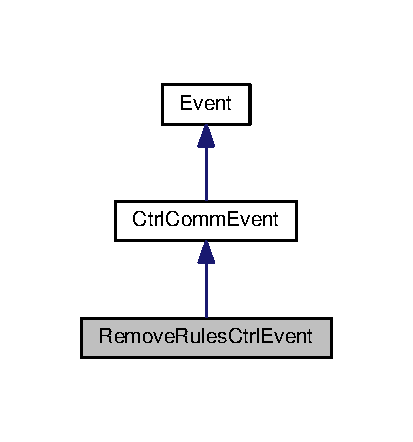
\includegraphics[width=198pt]{classRemoveRulesCtrlEvent__inherit__graph}
\end{center}
\end{figure}


Collaboration diagram for Remove\+Rules\+Ctrl\+Event\+:
\nopagebreak
\begin{figure}[H]
\begin{center}
\leavevmode
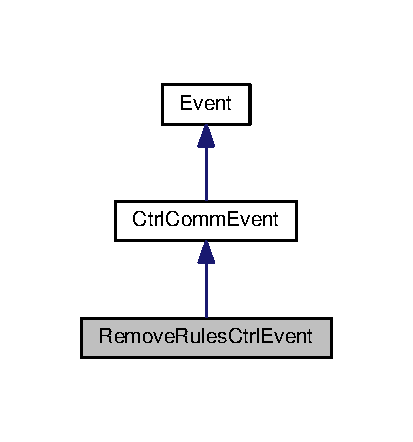
\includegraphics[width=198pt]{classRemoveRulesCtrlEvent__coll__graph}
\end{center}
\end{figure}
\subsection*{Public Member Functions}
\begin{DoxyCompactItemize}
\item 
\mbox{\Hypertarget{classRemoveRulesCtrlEvent_af97b2d469ae77d2af2accb3765fd8695}\label{classRemoveRulesCtrlEvent_af97b2d469ae77d2af2accb3765fd8695}} 
{\bfseries Remove\+Rules\+Ctrl\+Event} (string r)
\item 
\mbox{\Hypertarget{classRemoveRulesCtrlEvent_a0dfe839aad138da6212fb2f71add66f0}\label{classRemoveRulesCtrlEvent_a0dfe839aad138da6212fb2f71add66f0}} 
string {\bfseries get\+Rule} ()
\end{DoxyCompactItemize}


The documentation for this class was generated from the following file\+:\begin{DoxyCompactItemize}
\item 
include/\hyperlink{Event_8h}{Event.\+h}\end{DoxyCompactItemize}

\hypertarget{classRemoveRulesEvent}{}\section{Remove\+Rules\+Event Class Reference}
\label{classRemoveRulesEvent}\index{Remove\+Rules\+Event@{Remove\+Rules\+Event}}


Inheritance diagram for Remove\+Rules\+Event\+:
\nopagebreak
\begin{figure}[H]
\begin{center}
\leavevmode
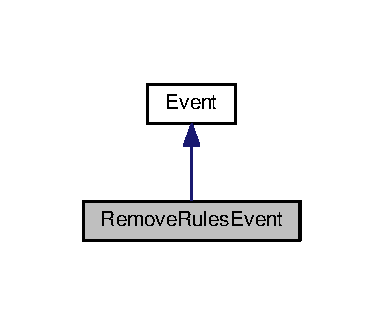
\includegraphics[width=184pt]{classRemoveRulesEvent__inherit__graph}
\end{center}
\end{figure}


Collaboration diagram for Remove\+Rules\+Event\+:
\nopagebreak
\begin{figure}[H]
\begin{center}
\leavevmode
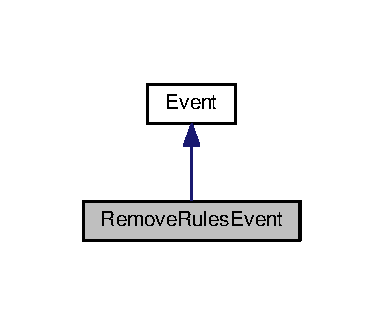
\includegraphics[width=184pt]{classRemoveRulesEvent__coll__graph}
\end{center}
\end{figure}
\subsection*{Public Member Functions}
\begin{DoxyCompactItemize}
\item 
\mbox{\Hypertarget{classRemoveRulesEvent_adf584666f47248f32fbbc2f1ebb9a313}\label{classRemoveRulesEvent_adf584666f47248f32fbbc2f1ebb9a313}} 
{\bfseries Remove\+Rules\+Event} (struct timeval time, \hyperlink{RuleFileParser_8h_a7d5bb94bb17a8a1d92db2a89a0cc96d1}{rule\+D\+B\+\_\+t} \&r)
\item 
\mbox{\Hypertarget{classRemoveRulesEvent_a7b3978a65ad21408bb5f1aa2e0650e17}\label{classRemoveRulesEvent_a7b3978a65ad21408bb5f1aa2e0650e17}} 
{\bfseries Remove\+Rules\+Event} (time\+\_\+t offs\+\_\+sec, \hyperlink{RuleFileParser_8h_a7d5bb94bb17a8a1d92db2a89a0cc96d1}{rule\+D\+B\+\_\+t} \&r)
\item 
\mbox{\Hypertarget{classRemoveRulesEvent_a00390e2cc409267037a13b42cf58bda5}\label{classRemoveRulesEvent_a00390e2cc409267037a13b42cf58bda5}} 
{\bfseries Remove\+Rules\+Event} (\hyperlink{RuleFileParser_8h_a7d5bb94bb17a8a1d92db2a89a0cc96d1}{rule\+D\+B\+\_\+t} \&r)
\item 
\mbox{\Hypertarget{classRemoveRulesEvent_aa0c839f29fc8421273128d261b2cea01}\label{classRemoveRulesEvent_aa0c839f29fc8421273128d261b2cea01}} 
\hyperlink{RuleFileParser_8h_a7d5bb94bb17a8a1d92db2a89a0cc96d1}{rule\+D\+B\+\_\+t} $\ast$ {\bfseries get\+Rules} ()
\item 
\mbox{\Hypertarget{classRemoveRulesEvent_aaf5e445b04a07dd2129d80e03ba43538}\label{classRemoveRulesEvent_aaf5e445b04a07dd2129d80e03ba43538}} 
int \hyperlink{classRemoveRulesEvent_aaf5e445b04a07dd2129d80e03ba43538}{delete\+Rule} (int uid)
\begin{DoxyCompactList}\small\item\em delete rules stored in this event \end{DoxyCompactList}\end{DoxyCompactItemize}


The documentation for this class was generated from the following file\+:\begin{DoxyCompactItemize}
\item 
include/\hyperlink{Event_8h}{Event.\+h}\end{DoxyCompactItemize}

\hypertarget{structREQUEST}{}\section{R\+E\+Q\+U\+E\+ST Struct Reference}
\label{structREQUEST}\index{R\+E\+Q\+U\+E\+ST@{R\+E\+Q\+U\+E\+ST}}


Collaboration diagram for R\+E\+Q\+U\+E\+ST\+:
\nopagebreak
\begin{figure}[H]
\begin{center}
\leavevmode
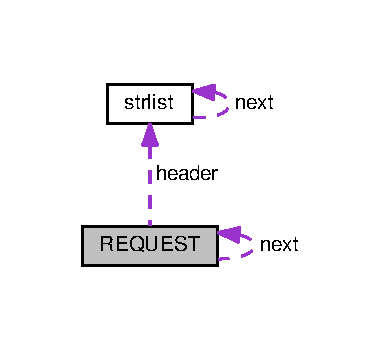
\includegraphics[width=184pt]{structREQUEST__coll__graph}
\end{center}
\end{figure}
\subsection*{Public Attributes}
\begin{DoxyCompactItemize}
\item 
\mbox{\Hypertarget{structREQUEST_a3b485c5abe81292e92ff442727806754}\label{structREQUEST_a3b485c5abe81292e92ff442727806754}} 
int {\bfseries fd}
\item 
\mbox{\Hypertarget{structREQUEST_ab9c9075cfcd3cd495d6e9d5426d145b6}\label{structREQUEST_ab9c9075cfcd3cd495d6e9d5426d145b6}} 
int {\bfseries state}
\item 
\mbox{\Hypertarget{structREQUEST_a2ba16f180a16587e066bd3c2d16d0355}\label{structREQUEST_a2ba16f180a16587e066bd3c2d16d0355}} 
time\+\_\+t {\bfseries ping}
\item 
\mbox{\Hypertarget{structREQUEST_a2c10c0657fe0fad2b7573ecf0e433bb1}\label{structREQUEST_a2c10c0657fe0fad2b7573ecf0e433bb1}} 
int {\bfseries keep\+\_\+alive}
\item 
\mbox{\Hypertarget{structREQUEST_a140da8d7b77f43baa5316923d585b105}\label{structREQUEST_a140da8d7b77f43baa5316923d585b105}} 
int {\bfseries tcp\+\_\+cork}
\item 
\mbox{\Hypertarget{structREQUEST_ad11be9186bf532496418f165541f56bb}\label{structREQUEST_ad11be9186bf532496418f165541f56bb}} 
struct sockaddr\+\_\+storage {\bfseries peer}
\item 
\mbox{\Hypertarget{structREQUEST_a546a43cb69b2526ab8b02f1ece5d7366}\label{structREQUEST_a546a43cb69b2526ab8b02f1ece5d7366}} 
char {\bfseries peerhost} \mbox{[}65\mbox{]}
\item 
\mbox{\Hypertarget{structREQUEST_a365b52befb639c4196ce9817da283d8f}\label{structREQUEST_a365b52befb639c4196ce9817da283d8f}} 
char {\bfseries peerserv} \mbox{[}9\mbox{]}
\item 
\mbox{\Hypertarget{structREQUEST_ad5dce0327433b4185779266aee5f2800}\label{structREQUEST_ad5dce0327433b4185779266aee5f2800}} 
char {\bfseries hreq} \mbox{[}M\+A\+X\+\_\+\+R\+EQ+1\mbox{]}
\item 
\mbox{\Hypertarget{structREQUEST_add195bdbe3e2fbd270d7a51c79f5f505}\label{structREQUEST_add195bdbe3e2fbd270d7a51c79f5f505}} 
int {\bfseries lreq}
\item 
\mbox{\Hypertarget{structREQUEST_a0b0b64b6be75f50ee5fe2200e9ec0fd4}\label{structREQUEST_a0b0b64b6be75f50ee5fe2200e9ec0fd4}} 
int {\bfseries hdata}
\item 
\mbox{\Hypertarget{structREQUEST_a4c62253b04825c33b5584e7dc0e68f80}\label{structREQUEST_a4c62253b04825c33b5584e7dc0e68f80}} 
char {\bfseries type} \mbox{[}16\mbox{]}
\item 
\mbox{\Hypertarget{structREQUEST_a6f4e6fd5433a9ebc38138ebf50a31227}\label{structREQUEST_a6f4e6fd5433a9ebc38138ebf50a31227}} 
char {\bfseries hostname} \mbox{[}65\mbox{]}
\item 
\mbox{\Hypertarget{structREQUEST_a67348c69ead30df6e151012b8a6d52b7}\label{structREQUEST_a67348c69ead30df6e151012b8a6d52b7}} 
char {\bfseries uri} \mbox{[}2049\mbox{]}
\item 
\mbox{\Hypertarget{structREQUEST_ab1720a44b923d21100cc1d3262eba0d4}\label{structREQUEST_ab1720a44b923d21100cc1d3262eba0d4}} 
char {\bfseries path} \mbox{[}2049\mbox{]}
\item 
\mbox{\Hypertarget{structREQUEST_a00ac50761cc623b6fabbe328d30fbb40}\label{structREQUEST_a00ac50761cc623b6fabbe328d30fbb40}} 
char {\bfseries query} \mbox{[}2049\mbox{]}
\item 
\mbox{\Hypertarget{structREQUEST_a2a2e887e5f6ec1ef31e4763e3160f654}\label{structREQUEST_a2a2e887e5f6ec1ef31e4763e3160f654}} 
int {\bfseries major}
\item 
\mbox{\Hypertarget{structREQUEST_a1d5635001426c8387fb15aad289c9555}\label{structREQUEST_a1d5635001426c8387fb15aad289c9555}} 
int {\bfseries minor}
\item 
\mbox{\Hypertarget{structREQUEST_acc1a0354ce44eb5d49aef39f4dba0054}\label{structREQUEST_acc1a0354ce44eb5d49aef39f4dba0054}} 
char {\bfseries auth} \mbox{[}64\mbox{]}
\item 
\mbox{\Hypertarget{structREQUEST_a9c01c1d5a6f76abe93383a520e60bcd7}\label{structREQUEST_a9c01c1d5a6f76abe93383a520e60bcd7}} 
struct \hyperlink{structstrlist}{strlist} $\ast$ {\bfseries header}
\item 
\mbox{\Hypertarget{structREQUEST_af3af7f2a9bcd3a10dff0ac2192ff7be8}\label{structREQUEST_af3af7f2a9bcd3a10dff0ac2192ff7be8}} 
time\+\_\+t {\bfseries if\+\_\+modified}
\item 
\mbox{\Hypertarget{structREQUEST_a7d53b97936ae2860024df2f034366863}\label{structREQUEST_a7d53b97936ae2860024df2f034366863}} 
time\+\_\+t {\bfseries if\+\_\+unmodified}
\item 
\mbox{\Hypertarget{structREQUEST_aa947afcf73e435e6d06dcfca3ac73d7f}\label{structREQUEST_aa947afcf73e435e6d06dcfca3ac73d7f}} 
time\+\_\+t {\bfseries if\+\_\+range}
\item 
\mbox{\Hypertarget{structREQUEST_a9ba7fb3102d52bd98b10474c3c03d270}\label{structREQUEST_a9ba7fb3102d52bd98b10474c3c03d270}} 
char $\ast$ {\bfseries range\+\_\+hdr}
\item 
\mbox{\Hypertarget{structREQUEST_a47997d3f103255c08e0c71f429e8b941}\label{structREQUEST_a47997d3f103255c08e0c71f429e8b941}} 
int {\bfseries ranges}
\item 
\mbox{\Hypertarget{structREQUEST_a015d2ced0aa1c92aca72047275ba229e}\label{structREQUEST_a015d2ced0aa1c92aca72047275ba229e}} 
off\+\_\+t $\ast$ {\bfseries r\+\_\+start}
\item 
\mbox{\Hypertarget{structREQUEST_a8d59a3471b45399b088c7535c6ac5306}\label{structREQUEST_a8d59a3471b45399b088c7535c6ac5306}} 
off\+\_\+t $\ast$ {\bfseries r\+\_\+end}
\item 
\mbox{\Hypertarget{structREQUEST_a9bcd9126993728e972739bd895ce352d}\label{structREQUEST_a9bcd9126993728e972739bd895ce352d}} 
char $\ast$ {\bfseries r\+\_\+head}
\item 
\mbox{\Hypertarget{structREQUEST_a0286f94c25843e6cc550cf876eb742b5}\label{structREQUEST_a0286f94c25843e6cc550cf876eb742b5}} 
int $\ast$ {\bfseries r\+\_\+hlen}
\item 
\mbox{\Hypertarget{structREQUEST_a52e3a0ae061025ce739d3c4e579824ea}\label{structREQUEST_a52e3a0ae061025ce739d3c4e579824ea}} 
char $\ast$ {\bfseries ctype}
\item 
\mbox{\Hypertarget{structREQUEST_ab990887c4c5749f38b672367157a2bc4}\label{structREQUEST_ab990887c4c5749f38b672367157a2bc4}} 
int {\bfseries clen}
\item 
\mbox{\Hypertarget{structREQUEST_a467d59c8ac16e1293d8a2f3ed07fb98f}\label{structREQUEST_a467d59c8ac16e1293d8a2f3ed07fb98f}} 
char $\ast$ {\bfseries breq}
\item 
\mbox{\Hypertarget{structREQUEST_ab0f360fe64122a0dc53c3a95cce99316}\label{structREQUEST_ab0f360fe64122a0dc53c3a95cce99316}} 
char {\bfseries post\+\_\+body} \mbox{[}M\+A\+X\+\_\+\+R\+EQ+1\mbox{]}
\item 
\mbox{\Hypertarget{structREQUEST_af73bf0e294b1ce30907a69d4429ed71a}\label{structREQUEST_af73bf0e294b1ce30907a69d4429ed71a}} 
int {\bfseries lbreq}
\item 
\mbox{\Hypertarget{structREQUEST_a50b812806152011a8b5bd0e703e01129}\label{structREQUEST_a50b812806152011a8b5bd0e703e01129}} 
int {\bfseries status}
\item 
\mbox{\Hypertarget{structREQUEST_a6f3abdf2f81ee491fc435a8d2cc6d950}\label{structREQUEST_a6f3abdf2f81ee491fc435a8d2cc6d950}} 
int {\bfseries bc}
\item 
\mbox{\Hypertarget{structREQUEST_a7148a81a780b72b65c7765d3367b90f2}\label{structREQUEST_a7148a81a780b72b65c7765d3367b90f2}} 
char {\bfseries hres} \mbox{[}M\+A\+X\+\_\+\+H\+E\+A\+D\+ER+1\mbox{]}
\item 
\mbox{\Hypertarget{structREQUEST_a51431e4cd1a57b66a56a114b130d89e8}\label{structREQUEST_a51431e4cd1a57b66a56a114b130d89e8}} 
int {\bfseries lres}
\item 
\mbox{\Hypertarget{structREQUEST_a1a5829da8a6051d7d86fdb454880a842}\label{structREQUEST_a1a5829da8a6051d7d86fdb454880a842}} 
char $\ast$ {\bfseries mime}
\item 
\mbox{\Hypertarget{structREQUEST_ac18f1048932b4f5b2d14b07e76bc594e}\label{structREQUEST_ac18f1048932b4f5b2d14b07e76bc594e}} 
char $\ast$ {\bfseries body}
\item 
\mbox{\Hypertarget{structREQUEST_a6de2692999bdfe8bb560a6ac55bf4f0a}\label{structREQUEST_a6de2692999bdfe8bb560a6ac55bf4f0a}} 
int {\bfseries lbody}
\item 
\mbox{\Hypertarget{structREQUEST_a00f3b53e23090d93f1fdc3dd2b3f89fd}\label{structREQUEST_a00f3b53e23090d93f1fdc3dd2b3f89fd}} 
int {\bfseries bfd}
\item 
\mbox{\Hypertarget{structREQUEST_a52eb8dbd37dcb50d6f4cbe07afa1b5a7}\label{structREQUEST_a52eb8dbd37dcb50d6f4cbe07afa1b5a7}} 
struct stat {\bfseries bst}
\item 
\mbox{\Hypertarget{structREQUEST_a71ec0a2a0f63900cbe4f55c9d34998bd}\label{structREQUEST_a71ec0a2a0f63900cbe4f55c9d34998bd}} 
off\+\_\+t {\bfseries written}
\item 
\mbox{\Hypertarget{structREQUEST_a45f97d1b901a6cf20b8c1afda8b6f544}\label{structREQUEST_a45f97d1b901a6cf20b8c1afda8b6f544}} 
int {\bfseries head\+\_\+only}
\item 
\mbox{\Hypertarget{structREQUEST_aae5661c09d2e7ca38d55ea5b30f1a291}\label{structREQUEST_aae5661c09d2e7ca38d55ea5b30f1a291}} 
int {\bfseries rh}
\item 
\mbox{\Hypertarget{structREQUEST_a2fc7edc7016483efbbaf9bc15d9962a7}\label{structREQUEST_a2fc7edc7016483efbbaf9bc15d9962a7}} 
int {\bfseries rb}
\item 
\mbox{\Hypertarget{structREQUEST_a3499889dcb97dce4efe1afa465479121}\label{structREQUEST_a3499889dcb97dce4efe1afa465479121}} 
int {\bfseries lifespan}
\item 
\mbox{\Hypertarget{structREQUEST_a89dad1805a6338683086a0c11e9bf57a}\label{structREQUEST_a89dad1805a6338683086a0c11e9bf57a}} 
struct \hyperlink{structREQUEST}{R\+E\+Q\+U\+E\+ST} $\ast$ {\bfseries next}
\end{DoxyCompactItemize}


The documentation for this struct was generated from the following file\+:\begin{DoxyCompactItemize}
\item 
lib/httpd/\hyperlink{httpd_8h}{httpd.\+h}\end{DoxyCompactItemize}

\hypertarget{classRule}{}\section{Rule Class Reference}
\label{classRule}\index{Rule@{Rule}}


parse and store a complete rule description  




{\ttfamily \#include $<$Rule.\+h$>$}

\subsection*{Public Member Functions}
\begin{DoxyCompactItemize}
\item 
\mbox{\Hypertarget{classRule_ab3da1447204ec745c198b78a45f58f5a}\label{classRule_ab3da1447204ec745c198b78a45f58f5a}} 
void {\bfseries set\+State} (\hyperlink{Rule_8h_ada0a7708a8188fca42891bcefcc55322}{rule\+State\+\_\+t} s)
\item 
\mbox{\Hypertarget{classRule_a77a8c310ca705429a6d083b8dcd81043}\label{classRule_a77a8c310ca705429a6d083b8dcd81043}} 
\hyperlink{Rule_8h_ada0a7708a8188fca42891bcefcc55322}{rule\+State\+\_\+t} {\bfseries get\+State} ()
\item 
\mbox{\Hypertarget{classRule_ae4709d88a7fe42b30488def531652b7d}\label{classRule_ae4709d88a7fe42b30488def531652b7d}} 
int {\bfseries is\+Flag\+Enabled} (rule\+Flags\+\_\+t f)
\item 
\mbox{\Hypertarget{classRule_abda94111e2d42e0719ff22f961de64a6}\label{classRule_abda94111e2d42e0719ff22f961de64a6}} 
int {\bfseries get\+U\+Id} ()
\item 
\mbox{\Hypertarget{classRule_ac7a9ed77e78ecd7bd35887fba4ad44d0}\label{classRule_ac7a9ed77e78ecd7bd35887fba4ad44d0}} 
void {\bfseries set\+U\+Id} (int nuid)
\item 
\mbox{\Hypertarget{classRule_a9e442e10cbbb90ea94de2bf931120662}\label{classRule_a9e442e10cbbb90ea94de2bf931120662}} 
string {\bfseries get\+Set\+Name} ()
\item 
\mbox{\Hypertarget{classRule_a4fb86d5cc62efdd5c6dd44dfde8fbdba}\label{classRule_a4fb86d5cc62efdd5c6dd44dfde8fbdba}} 
string {\bfseries get\+Rule\+Name} ()
\item 
\mbox{\Hypertarget{classRule_ae2d8226afc17d3f0d661b2d462d4c7eb}\label{classRule_ae2d8226afc17d3f0d661b2d462d4c7eb}} 
string {\bfseries get\+Rule\+Source} ()
\item 
\mbox{\Hypertarget{classRule_ab6751b839ab0a0538fc2d29d85cf2fff}\label{classRule_ab6751b839ab0a0538fc2d29d85cf2fff}} 
string {\bfseries get\+Rule\+Id} ()
\item 
\mbox{\Hypertarget{classRule_ab3f161d40bc42df2be8886ba0c4d0b6b}\label{classRule_ab3f161d40bc42df2be8886ba0c4d0b6b}} 
time\+\_\+t {\bfseries get\+Start} ()
\item 
\mbox{\Hypertarget{classRule_a49feb39c6002b2522d042c21f5c8afcd}\label{classRule_a49feb39c6002b2522d042c21f5c8afcd}} 
time\+\_\+t {\bfseries get\+Stop} ()
\item 
\mbox{\Hypertarget{classRule_a80e16da3df683cb2777511fd98cfdec2}\label{classRule_a80e16da3df683cb2777511fd98cfdec2}} 
int {\bfseries is\+Bidir} ()
\item 
\mbox{\Hypertarget{classRule_ad6eb30b824e19044b1190beae6febebe}\label{classRule_ad6eb30b824e19044b1190beae6febebe}} 
int {\bfseries sep\+Paths} ()
\item 
\mbox{\Hypertarget{classRule_af9b6211b0c4cdcbf84450718d2c65457}\label{classRule_af9b6211b0c4cdcbf84450718d2c65457}} 
void {\bfseries set\+Bidir} ()
\item 
\mbox{\Hypertarget{classRule_af550df52b67018330bfad8b7fabd3210}\label{classRule_af550df52b67018330bfad8b7fabd3210}} 
unsigned long {\bfseries get\+Flow\+Timeout} ()
\item 
\hyperlink{classRule_af5a5d5dedcf5fce8b376e1041df916f6}{Rule} (int \+\_\+uid, time\+\_\+t now, string sname, string rname, \hyperlink{ProcModuleInterface_8h_a2afc1e9fc63b2cfcd86ec2435f24e27c}{filter\+List\+\_\+t} \&f, \hyperlink{Rule_8h_acdc7809742ec5b554bf13b4c12053a6a}{action\+List\+\_\+t} \&a, \hyperlink{Rule_8h_a9fb303c0fc85a5e78d6d35728fe7fe74}{misc\+List\+\_\+t} \&m)
\begin{DoxyCompactList}\small\item\em construct and initialize a \hyperlink{classRule}{Rule} object \end{DoxyCompactList}\item 
\mbox{\Hypertarget{classRule_a92760fc705b3da696f86e42b77943c21}\label{classRule_a92760fc705b3da696f86e42b77943c21}} 
\hyperlink{classRule_a92760fc705b3da696f86e42b77943c21}{$\sim$\+Rule} ()
\begin{DoxyCompactList}\small\item\em destroy a \hyperlink{classRule}{Rule} object \end{DoxyCompactList}\item 
\hyperlink{Rule_8h_acdc7809742ec5b554bf13b4c12053a6a}{action\+List\+\_\+t} $\ast$ \hyperlink{classRule_a2537cf47f367282809a66f9bfb733020}{get\+Actions} ()
\begin{DoxyCompactList}\small\item\em get names and values (parameters) of configured actions \end{DoxyCompactList}\item 
\hyperlink{ProcModuleInterface_8h_a2afc1e9fc63b2cfcd86ec2435f24e27c}{filter\+List\+\_\+t} $\ast$ \hyperlink{classRule_ad247112cb17b723d048dadf4afe34fa6}{get\+Filter} ()
\begin{DoxyCompactList}\small\item\em get names and values (parameters) of configured filter rule \end{DoxyCompactList}\item 
\hyperlink{Rule_8h_a9fb303c0fc85a5e78d6d35728fe7fe74}{misc\+List\+\_\+t} $\ast$ \hyperlink{classRule_a37927201f07b2990cdd342162c7ddf96}{get\+Misc} ()
\begin{DoxyCompactList}\small\item\em get names and values (parameters) of misc. attributes \end{DoxyCompactList}\item 
\mbox{\Hypertarget{classRule_ac88b5cc900b2e39dc3c674bb259f1e86}\label{classRule_ac88b5cc900b2e39dc3c674bb259f1e86}} 
void \hyperlink{classRule_ac88b5cc900b2e39dc3c674bb259f1e86}{dump} (ostream \&os)
\begin{DoxyCompactList}\small\item\em dump a \hyperlink{classRule}{Rule} object \end{DoxyCompactList}\item 
\mbox{\Hypertarget{classRule_ac67bda46af62221c2e02e5338b47cc6a}\label{classRule_ac67bda46af62221c2e02e5338b47cc6a}} 
string \hyperlink{classRule_ac67bda46af62221c2e02e5338b47cc6a}{get\+Info} (void)
\begin{DoxyCompactList}\small\item\em get rule info string \end{DoxyCompactList}\end{DoxyCompactItemize}


\subsection{Detailed Description}
parse and store a complete rule description 

\subsection{Constructor \& Destructor Documentation}
\mbox{\Hypertarget{classRule_af5a5d5dedcf5fce8b376e1041df916f6}\label{classRule_af5a5d5dedcf5fce8b376e1041df916f6}} 
\index{Rule@{Rule}!Rule@{Rule}}
\index{Rule@{Rule}!Rule@{Rule}}
\subsubsection{\texorpdfstring{Rule()}{Rule()}}
{\footnotesize\ttfamily Rule\+::\+Rule (\begin{DoxyParamCaption}\item[{int}]{\+\_\+uid,  }\item[{time\+\_\+t}]{now,  }\item[{string}]{sname,  }\item[{string}]{rname,  }\item[{\hyperlink{ProcModuleInterface_8h_a2afc1e9fc63b2cfcd86ec2435f24e27c}{filter\+List\+\_\+t} \&}]{f,  }\item[{\hyperlink{Rule_8h_acdc7809742ec5b554bf13b4c12053a6a}{action\+List\+\_\+t} \&}]{a,  }\item[{\hyperlink{Rule_8h_a9fb303c0fc85a5e78d6d35728fe7fe74}{misc\+List\+\_\+t} \&}]{m }\end{DoxyParamCaption})}



construct and initialize a \hyperlink{classRule}{Rule} object 

\begin{DoxyItemize}
\item {\ttfamily now} current timestamp \item {\ttfamily sname} rule set name \item {\ttfamily s} rname rule name \item {\ttfamily f} list of filters \item {\ttfamily a} list of actions \item {\ttfamily e} list of exports \item {\ttfamily m} list of misc parameters \end{DoxyItemize}


\subsection{Member Function Documentation}
\mbox{\Hypertarget{classRule_a2537cf47f367282809a66f9bfb733020}\label{classRule_a2537cf47f367282809a66f9bfb733020}} 
\index{Rule@{Rule}!get\+Actions@{get\+Actions}}
\index{get\+Actions@{get\+Actions}!Rule@{Rule}}
\subsubsection{\texorpdfstring{get\+Actions()}{getActions()}}
{\footnotesize\ttfamily \hyperlink{Rule_8h_acdc7809742ec5b554bf13b4c12053a6a}{action\+List\+\_\+t} $\ast$ Rule\+::get\+Actions (\begin{DoxyParamCaption}{ }\end{DoxyParamCaption})}



get names and values (parameters) of configured actions 

\begin{DoxyReturn}{Returns}
a pointer (link) to a list that contains the configured actions for this rule 
\end{DoxyReturn}
\mbox{\Hypertarget{classRule_ad247112cb17b723d048dadf4afe34fa6}\label{classRule_ad247112cb17b723d048dadf4afe34fa6}} 
\index{Rule@{Rule}!get\+Filter@{get\+Filter}}
\index{get\+Filter@{get\+Filter}!Rule@{Rule}}
\subsubsection{\texorpdfstring{get\+Filter()}{getFilter()}}
{\footnotesize\ttfamily \hyperlink{ProcModuleInterface_8h_a2afc1e9fc63b2cfcd86ec2435f24e27c}{filter\+List\+\_\+t} $\ast$ Rule\+::get\+Filter (\begin{DoxyParamCaption}{ }\end{DoxyParamCaption})}



get names and values (parameters) of configured filter rule 

\begin{DoxyReturn}{Returns}
a pointer (link) to a Parameter\+Set object that contains the configured filter rule description for this rule 
\end{DoxyReturn}
\mbox{\Hypertarget{classRule_a37927201f07b2990cdd342162c7ddf96}\label{classRule_a37927201f07b2990cdd342162c7ddf96}} 
\index{Rule@{Rule}!get\+Misc@{get\+Misc}}
\index{get\+Misc@{get\+Misc}!Rule@{Rule}}
\subsubsection{\texorpdfstring{get\+Misc()}{getMisc()}}
{\footnotesize\ttfamily \hyperlink{Rule_8h_a9fb303c0fc85a5e78d6d35728fe7fe74}{misc\+List\+\_\+t} $\ast$ Rule\+::get\+Misc (\begin{DoxyParamCaption}{ }\end{DoxyParamCaption})}



get names and values (parameters) of misc. attributes 

\begin{DoxyReturn}{Returns}
a pointer (link) to a Parameter\+Set object that contains the miscanellenous attributes of a configured filter rule 
\end{DoxyReturn}


The documentation for this class was generated from the following files\+:\begin{DoxyCompactItemize}
\item 
include/\hyperlink{Rule_8h}{Rule.\+h}\item 
src/\hyperlink{Rule_8cpp}{Rule.\+cpp}\end{DoxyCompactItemize}

\hypertarget{structruleActions__t}{}\section{rule\+Actions\+\_\+t Struct Reference}
\label{structruleActions__t}\index{rule\+Actions\+\_\+t@{rule\+Actions\+\_\+t}}


Collaboration diagram for rule\+Actions\+\_\+t\+:
\nopagebreak
\begin{figure}[H]
\begin{center}
\leavevmode
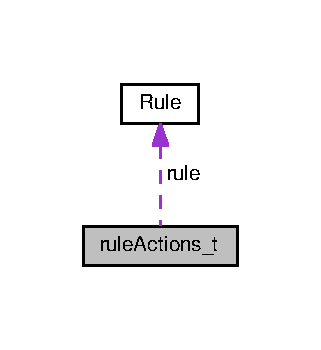
\includegraphics[width=154pt]{structruleActions__t__coll__graph}
\end{center}
\end{figure}
\subsection*{Public Attributes}
\begin{DoxyCompactItemize}
\item 
time\+\_\+t \hyperlink{structruleActions__t_ab5d6b8c4bc751e5db10186fdb6d7757f}{last\+Pkt}
\item 
\mbox{\Hypertarget{structruleActions__t_ae05927277834557d602b60bb61d59528}\label{structruleActions__t_ae05927277834557d602b60bb61d59528}} 
unsigned long long \hyperlink{structruleActions__t_ae05927277834557d602b60bb61d59528}{packets}
\begin{DoxyCompactList}\small\item\em number of packets and bytes seen by this rule/task \end{DoxyCompactList}\item 
\mbox{\Hypertarget{structruleActions__t_a077726e7d244280e177c7c3c5365787c}\label{structruleActions__t_a077726e7d244280e177c7c3c5365787c}} 
unsigned long long {\bfseries bytes}
\item 
\mbox{\Hypertarget{structruleActions__t_a8c9d9225770b1beeb2aed2b1a5c1dd97}\label{structruleActions__t_a8c9d9225770b1beeb2aed2b1a5c1dd97}} 
\hyperlink{QOSProcessor_8h_ae32981e3c7557573d2a6a8f1694c3e5f}{ppaction\+List\+\_\+t} {\bfseries actions}
\item 
\mbox{\Hypertarget{structruleActions__t_a94de4fb69b43a5f3ca25eaefb67dbd53}\label{structruleActions__t_a94de4fb69b43a5f3ca25eaefb67dbd53}} 
int {\bfseries auto\+\_\+flows}
\item 
\mbox{\Hypertarget{structruleActions__t_af377e0b9445f20822e3a66a2e59940bc}\label{structruleActions__t_af377e0b9445f20822e3a66a2e59940bc}} 
int {\bfseries bidir}
\item 
\mbox{\Hypertarget{structruleActions__t_ad900355420b0afe0b4beb3a824c48c56}\label{structruleActions__t_ad900355420b0afe0b4beb3a824c48c56}} 
int {\bfseries seppaths}
\item 
\mbox{\Hypertarget{structruleActions__t_a4dd9a5c819dc8674697d6497adce29a8}\label{structruleActions__t_a4dd9a5c819dc8674697d6497adce29a8}} 
\hyperlink{classRule}{Rule} $\ast$ {\bfseries rule}
\item 
\mbox{\Hypertarget{structruleActions__t_a5bb1477b49fa6cb59c6a25e0eb2d1ab6}\label{structruleActions__t_a5bb1477b49fa6cb59c6a25e0eb2d1ab6}} 
\hyperlink{ProcModuleInterface_8h_a2afc1e9fc63b2cfcd86ec2435f24e27c}{filter\+List\+\_\+t} $\ast$ {\bfseries flist}
\end{DoxyCompactItemize}


\subsection{Member Data Documentation}
\mbox{\Hypertarget{structruleActions__t_ab5d6b8c4bc751e5db10186fdb6d7757f}\label{structruleActions__t_ab5d6b8c4bc751e5db10186fdb6d7757f}} 
\index{rule\+Actions\+\_\+t@{rule\+Actions\+\_\+t}!last\+Pkt@{last\+Pkt}}
\index{last\+Pkt@{last\+Pkt}!rule\+Actions\+\_\+t@{rule\+Actions\+\_\+t}}
\subsubsection{\texorpdfstring{last\+Pkt}{lastPkt}}
{\footnotesize\ttfamily time\+\_\+t rule\+Actions\+\_\+t\+::last\+Pkt}

time stamp of last packet seen for the packet flow of this task =0 indicates the flow was set to idle previously 

The documentation for this struct was generated from the following file\+:\begin{DoxyCompactItemize}
\item 
include/\hyperlink{QOSProcessor_8h}{Q\+O\+S\+Processor.\+h}\end{DoxyCompactItemize}

\hypertarget{classRuleFileParser}{}\section{Rule\+File\+Parser Class Reference}
\label{classRuleFileParser}\index{Rule\+File\+Parser@{Rule\+File\+Parser}}


Inheritance diagram for Rule\+File\+Parser\+:
\nopagebreak
\begin{figure}[H]
\begin{center}
\leavevmode
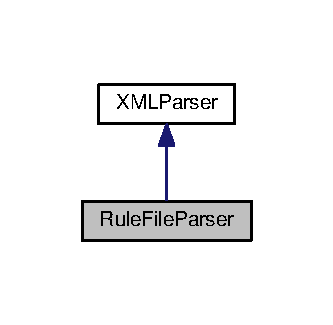
\includegraphics[width=160pt]{classRuleFileParser__inherit__graph}
\end{center}
\end{figure}


Collaboration diagram for Rule\+File\+Parser\+:
\nopagebreak
\begin{figure}[H]
\begin{center}
\leavevmode
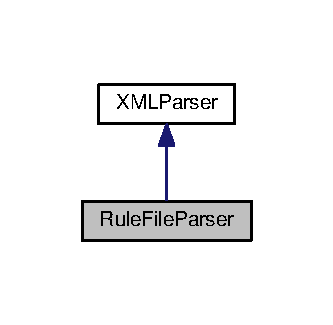
\includegraphics[width=160pt]{classRuleFileParser__coll__graph}
\end{center}
\end{figure}
\subsection*{Public Member Functions}
\begin{DoxyCompactItemize}
\item 
\mbox{\Hypertarget{classRuleFileParser_a6386e0976c97bbf050bd46613754bf0f}\label{classRuleFileParser_a6386e0976c97bbf050bd46613754bf0f}} 
{\bfseries Rule\+File\+Parser} (string fname)
\item 
\mbox{\Hypertarget{classRuleFileParser_a937b90925b91fd4a36683e8bfd9188ac}\label{classRuleFileParser_a937b90925b91fd4a36683e8bfd9188ac}} 
{\bfseries Rule\+File\+Parser} (char $\ast$buf, int len)
\item 
\mbox{\Hypertarget{classRuleFileParser_a698a0f3db42a256169191e3d6c52d559}\label{classRuleFileParser_a698a0f3db42a256169191e3d6c52d559}} 
virtual void \hyperlink{classRuleFileParser_a698a0f3db42a256169191e3d6c52d559}{parse} (filter\+Def\+List\+\_\+t $\ast$filters, filter\+Val\+List\+\_\+t $\ast$filter\+Vals, \hyperlink{RuleFileParser_8h_a7d5bb94bb17a8a1d92db2a89a0cc96d1}{rule\+D\+B\+\_\+t} $\ast$rules, \hyperlink{classRuleIdSource}{Rule\+Id\+Source} $\ast$id\+Source)
\begin{DoxyCompactList}\small\item\em parse rules and add parsed rules to the list of rules \end{DoxyCompactList}\end{DoxyCompactItemize}
\subsection*{Additional Inherited Members}


The documentation for this class was generated from the following files\+:\begin{DoxyCompactItemize}
\item 
include/\hyperlink{RuleFileParser_8h}{Rule\+File\+Parser.\+h}\item 
src/\hyperlink{RuleFileParser_8cpp}{Rule\+File\+Parser.\+cpp}\end{DoxyCompactItemize}

\hypertarget{classRuleIdSource}{}\section{Rule\+Id\+Source Class Reference}
\label{classRuleIdSource}\index{Rule\+Id\+Source@{Rule\+Id\+Source}}


generate unique id numbers  




{\ttfamily \#include $<$Rule\+Id\+Source.\+h$>$}

\subsection*{Public Member Functions}
\begin{DoxyCompactItemize}
\item 
\hyperlink{classRuleIdSource_aae6bfb7f53dc67d7a2700736c330c443}{Rule\+Id\+Source} (int unique=0)
\item 
\mbox{\Hypertarget{classRuleIdSource_a6fb34a092990296a8998cb5877adcec3}\label{classRuleIdSource_a6fb34a092990296a8998cb5877adcec3}} 
\hyperlink{classRuleIdSource_a6fb34a092990296a8998cb5877adcec3}{$\sim$\+Rule\+Id\+Source} ()
\begin{DoxyCompactList}\small\item\em destroy a \hyperlink{classRuleIdSource}{Rule\+Id\+Source} object \end{DoxyCompactList}\item 
unsigned short \hyperlink{classRuleIdSource_a1c4a3c9ff759ed7b4ba77f3331e1b7d0}{new\+Id} (void)
\begin{DoxyCompactList}\small\item\em generate a new internal id number \end{DoxyCompactList}\item 
void \hyperlink{classRuleIdSource_a81879127eea335cb4722c42915e4712e}{free\+Id} (unsigned short id)
\begin{DoxyCompactList}\small\item\em release an id number \end{DoxyCompactList}\item 
\mbox{\Hypertarget{classRuleIdSource_a5127a27a536916b11a7becc6921c929c}\label{classRuleIdSource_a5127a27a536916b11a7becc6921c929c}} 
void \hyperlink{classRuleIdSource_a5127a27a536916b11a7becc6921c929c}{dump} (ostream \&os)
\begin{DoxyCompactList}\small\item\em dump a \hyperlink{classRuleIdSource}{Rule\+Id\+Source} object \end{DoxyCompactList}\end{DoxyCompactItemize}


\subsection{Detailed Description}
generate unique id numbers 

The \hyperlink{classRuleIdSource}{Rule\+Id\+Source} class can generate unique 32 bit integer numbers for use by other functions. A single number can be lent from the pool of available numbers, and this number will not be generated by a call to the new\+Id function until it has been previously released with a call to the free\+Id function. 

\subsection{Constructor \& Destructor Documentation}
\mbox{\Hypertarget{classRuleIdSource_aae6bfb7f53dc67d7a2700736c330c443}\label{classRuleIdSource_aae6bfb7f53dc67d7a2700736c330c443}} 
\index{Rule\+Id\+Source@{Rule\+Id\+Source}!Rule\+Id\+Source@{Rule\+Id\+Source}}
\index{Rule\+Id\+Source@{Rule\+Id\+Source}!Rule\+Id\+Source@{Rule\+Id\+Source}}
\subsubsection{\texorpdfstring{Rule\+Id\+Source()}{RuleIdSource()}}
{\footnotesize\ttfamily Rule\+Id\+Source\+::\+Rule\+Id\+Source (\begin{DoxyParamCaption}\item[{int}]{unique = {\ttfamily 0} }\end{DoxyParamCaption})}

construct and initialize a \hyperlink{classRuleIdSource}{Rule\+Id\+Source} object if unique is set to 1 Ids should be unique until we wrap around 2$^\wedge$16 We remove ids numbered\+: 0 -- Reserved for qdisc 1 -- Reserved for root class 0x\+F\+F\+FF -- Reserved for default class 

\subsection{Member Function Documentation}
\mbox{\Hypertarget{classRuleIdSource_a81879127eea335cb4722c42915e4712e}\label{classRuleIdSource_a81879127eea335cb4722c42915e4712e}} 
\index{Rule\+Id\+Source@{Rule\+Id\+Source}!free\+Id@{free\+Id}}
\index{free\+Id@{free\+Id}!Rule\+Id\+Source@{Rule\+Id\+Source}}
\subsubsection{\texorpdfstring{free\+Id()}{freeId()}}
{\footnotesize\ttfamily void Rule\+Id\+Source\+::free\+Id (\begin{DoxyParamCaption}\item[{unsigned short}]{id }\end{DoxyParamCaption})}



release an id number 

The released id number can be reused (i.\+e. returned by new\+Id) after the call to free\+Id. Do not release numbers that have not been obtained by a call to new\+Id this will result in unpredictable behaviour.

\begin{DoxyItemize}
\item {\ttfamily id} -\/ id value that is to be released for future use \end{DoxyItemize}
\mbox{\Hypertarget{classRuleIdSource_a1c4a3c9ff759ed7b4ba77f3331e1b7d0}\label{classRuleIdSource_a1c4a3c9ff759ed7b4ba77f3331e1b7d0}} 
\index{Rule\+Id\+Source@{Rule\+Id\+Source}!new\+Id@{new\+Id}}
\index{new\+Id@{new\+Id}!Rule\+Id\+Source@{Rule\+Id\+Source}}
\subsubsection{\texorpdfstring{new\+Id()}{newId()}}
{\footnotesize\ttfamily unsigned short Rule\+Id\+Source\+::new\+Id (\begin{DoxyParamCaption}\item[{void}]{ }\end{DoxyParamCaption})}



generate a new internal id number 

return a new Id value that is currently not in use. This value will be marked as used and will not returned by a call to new\+Id unless it has been released again with a call to free\+Id \begin{DoxyReturn}{Returns}
unique unused id value 
\end{DoxyReturn}


The documentation for this class was generated from the following files\+:\begin{DoxyCompactItemize}
\item 
include/\hyperlink{RuleIdSource_8h}{Rule\+Id\+Source.\+h}\item 
src/\hyperlink{RuleIdSource_8cpp}{Rule\+Id\+Source.\+cpp}\end{DoxyCompactItemize}

\hypertarget{classRuleManager}{}\section{Rule\+Manager Class Reference}
\label{classRuleManager}\index{Rule\+Manager@{Rule\+Manager}}


manage adding/deleting of complete rule descriptions  




{\ttfamily \#include $<$Rule\+Manager.\+h$>$}

\subsection*{Public Member Functions}
\begin{DoxyCompactItemize}
\item 
\mbox{\Hypertarget{classRuleManager_a21d68fb7fdaa507fafd5ff6099381cc1}\label{classRuleManager_a21d68fb7fdaa507fafd5ff6099381cc1}} 
int {\bfseries get\+Num\+Tasks} ()
\item 
\mbox{\Hypertarget{classRuleManager_abea1764880229293d1f864fb0748657f}\label{classRuleManager_abea1764880229293d1f864fb0748657f}} 
filter\+Def\+List\+\_\+t $\ast$ {\bfseries get\+Filter\+Defs} ()
\item 
\mbox{\Hypertarget{classRuleManager_a838212711c14ca2708c861c8a5791807}\label{classRuleManager_a838212711c14ca2708c861c8a5791807}} 
string {\bfseries get\+Info} (int uid)
\item 
\hyperlink{classRuleManager_a31bcd41f979a78dcdeb9dcfc2460aa15}{Rule\+Manager} (string fdname, string fvname)
\begin{DoxyCompactList}\small\item\em construct and initialize a \hyperlink{classRuleManager}{Rule\+Manager} object \end{DoxyCompactList}\item 
\mbox{\Hypertarget{classRuleManager_a5c957ab5466f026a427727655c2f577c}\label{classRuleManager_a5c957ab5466f026a427727655c2f577c}} 
\hyperlink{classRuleManager_a5c957ab5466f026a427727655c2f577c}{$\sim$\+Rule\+Manager} ()
\begin{DoxyCompactList}\small\item\em destroy a \hyperlink{classRuleManager}{Rule\+Manager} object \end{DoxyCompactList}\item 
\hyperlink{classRule}{Rule} $\ast$ \hyperlink{classRuleManager_ab081c7bea7b31ff32059c1b470b6208d}{get\+Rule} (int uid)
\begin{DoxyCompactList}\small\item\em lookup the rule info data for a given rule\+Id or name \end{DoxyCompactList}\item 
\mbox{\Hypertarget{classRuleManager_aa7ce90c80d7c6e167d5fe396b9310985}\label{classRuleManager_aa7ce90c80d7c6e167d5fe396b9310985}} 
\hyperlink{classRule}{Rule} $\ast$ \hyperlink{classRuleManager_aa7ce90c80d7c6e167d5fe396b9310985}{get\+Rule} (string sname, string rname)
\begin{DoxyCompactList}\small\item\em get rule rname from ruleset sname \end{DoxyCompactList}\item 
\mbox{\Hypertarget{classRuleManager_abe81485b01b2db580370da44f0d86f37}\label{classRuleManager_abe81485b01b2db580370da44f0d86f37}} 
rule\+Index\+\_\+t $\ast$ \hyperlink{classRuleManager_abe81485b01b2db580370da44f0d86f37}{get\+Rules} (string sname)
\begin{DoxyCompactList}\small\item\em get all rules in ruleset with name sname \end{DoxyCompactList}\item 
\mbox{\Hypertarget{classRuleManager_ac2968da0034fbf6603f08b8b83817a0a}\label{classRuleManager_ac2968da0034fbf6603f08b8b83817a0a}} 
\hyperlink{RuleFileParser_8h_a7d5bb94bb17a8a1d92db2a89a0cc96d1}{rule\+D\+B\+\_\+t} \hyperlink{classRuleManager_ac2968da0034fbf6603f08b8b83817a0a}{get\+Rules} ()
\begin{DoxyCompactList}\small\item\em get all rules \end{DoxyCompactList}\item 
\mbox{\Hypertarget{classRuleManager_a90df59d4ab10d4e31e239c1a136bd410}\label{classRuleManager_a90df59d4ab10d4e31e239c1a136bd410}} 
\hyperlink{RuleFileParser_8h_a7d5bb94bb17a8a1d92db2a89a0cc96d1}{rule\+D\+B\+\_\+t} $\ast$ \hyperlink{classRuleManager_a90df59d4ab10d4e31e239c1a136bd410}{parse\+Rules} (string fname)
\begin{DoxyCompactList}\small\item\em parse X\+ML rules from file \end{DoxyCompactList}\item 
\mbox{\Hypertarget{classRuleManager_a79c110f6566aab42fbab44d9efbc449f}\label{classRuleManager_a79c110f6566aab42fbab44d9efbc449f}} 
\hyperlink{RuleFileParser_8h_a7d5bb94bb17a8a1d92db2a89a0cc96d1}{rule\+D\+B\+\_\+t} $\ast$ \hyperlink{classRuleManager_a79c110f6566aab42fbab44d9efbc449f}{parse\+Rules\+Buffer} (char $\ast$buf, int len, int mapi)
\begin{DoxyCompactList}\small\item\em parse X\+ML or Meter A\+PI rules from buffer \end{DoxyCompactList}\item 
void \hyperlink{classRuleManager_ae1d3a7b7e4ccf47a992e8239d3f643a4}{add\+Rules} (\hyperlink{RuleFileParser_8h_a7d5bb94bb17a8a1d92db2a89a0cc96d1}{rule\+D\+B\+\_\+t} $\ast$rules, \hyperlink{classEventScheduler}{Event\+Scheduler} $\ast$e)
\begin{DoxyCompactList}\small\item\em add a filter rule description \end{DoxyCompactList}\item 
\mbox{\Hypertarget{classRuleManager_a40a2dd1e2f15f37c2237079b431bccd8}\label{classRuleManager_a40a2dd1e2f15f37c2237079b431bccd8}} 
void \hyperlink{classRuleManager_a40a2dd1e2f15f37c2237079b431bccd8}{add\+Rule} (\hyperlink{classRule}{Rule} $\ast$r)
\begin{DoxyCompactList}\small\item\em add a single rule \end{DoxyCompactList}\item 
\mbox{\Hypertarget{classRuleManager_a7318810cdd95a602ce890afe2b603320}\label{classRuleManager_a7318810cdd95a602ce890afe2b603320}} 
void \hyperlink{classRuleManager_a7318810cdd95a602ce890afe2b603320}{activate\+Rules} (\hyperlink{RuleFileParser_8h_a7d5bb94bb17a8a1d92db2a89a0cc96d1}{rule\+D\+B\+\_\+t} $\ast$rules, \hyperlink{classEventScheduler}{Event\+Scheduler} $\ast$e)
\begin{DoxyCompactList}\small\item\em activate/execute rules \end{DoxyCompactList}\item 
void \hyperlink{classRuleManager_ab01b6ffe72edce8b9d8b8d3ff5baf55b}{del\+Rule} (int uid, \hyperlink{classEventScheduler}{Event\+Scheduler} $\ast$e)
\begin{DoxyCompactList}\small\item\em delete a filter rule description \end{DoxyCompactList}\item 
\mbox{\Hypertarget{classRuleManager_ac1b0013d3bb1d153ff5eaee4974ea275}\label{classRuleManager_ac1b0013d3bb1d153ff5eaee4974ea275}} 
void {\bfseries del\+Rule} (string rname, string sname, \hyperlink{classEventScheduler}{Event\+Scheduler} $\ast$e)
\item 
\mbox{\Hypertarget{classRuleManager_aee617ae038c13cd8a0aa292b6a16c325}\label{classRuleManager_aee617ae038c13cd8a0aa292b6a16c325}} 
void {\bfseries del\+Rules} (string sname, \hyperlink{classEventScheduler}{Event\+Scheduler} $\ast$e)
\item 
\mbox{\Hypertarget{classRuleManager_aebb5b47bca52719f5741039002d7a9f8}\label{classRuleManager_aebb5b47bca52719f5741039002d7a9f8}} 
void {\bfseries del\+Rule} (\hyperlink{classRule}{Rule} $\ast$r, \hyperlink{classEventScheduler}{Event\+Scheduler} $\ast$e)
\item 
\mbox{\Hypertarget{classRuleManager_ac6780adf74bf7918005086a594aa1df0}\label{classRuleManager_ac6780adf74bf7918005086a594aa1df0}} 
void {\bfseries del\+Rules} (\hyperlink{RuleFileParser_8h_a7d5bb94bb17a8a1d92db2a89a0cc96d1}{rule\+D\+B\+\_\+t} $\ast$rules, \hyperlink{classEventScheduler}{Event\+Scheduler} $\ast$e)
\item 
string \hyperlink{classRuleManager_a15995aaed6daab992a46aeeac5d54e06}{get\+Info} (void)
\begin{DoxyCompactList}\small\item\em get information from the rule manager \end{DoxyCompactList}\item 
\mbox{\Hypertarget{classRuleManager_a4202560315a439c6359587b08fe4df97}\label{classRuleManager_a4202560315a439c6359587b08fe4df97}} 
string {\bfseries get\+Info} (\hyperlink{classRule}{Rule} $\ast$r)
\item 
\mbox{\Hypertarget{classRuleManager_aceef53a03385cd8ea5ee84c679f8cb82}\label{classRuleManager_aceef53a03385cd8ea5ee84c679f8cb82}} 
string {\bfseries get\+Info} (string sname, string rname)
\item 
\mbox{\Hypertarget{classRuleManager_aa7b8b1de53715c8a63d88812f858c9ee}\label{classRuleManager_aa7b8b1de53715c8a63d88812f858c9ee}} 
string {\bfseries get\+Info} (string sname)
\item 
\mbox{\Hypertarget{classRuleManager_a09bd92aa70fdd885ee877d1e2a108d11}\label{classRuleManager_a09bd92aa70fdd885ee877d1e2a108d11}} 
void \hyperlink{classRuleManager_a09bd92aa70fdd885ee877d1e2a108d11}{dump} (ostream \&os)
\begin{DoxyCompactList}\small\item\em dump a \hyperlink{classRuleManager}{Rule\+Manager} object \end{DoxyCompactList}\end{DoxyCompactItemize}


\subsection{Detailed Description}
manage adding/deleting of complete rule descriptions 

the \hyperlink{classRuleManager}{Rule\+Manager} class allows to add and remove rules in the Meters core system. \hyperlink{classRule}{Rule} data are a set of ascii strings that are parsed and syntax checked by the \hyperlink{classRuleManager}{Rule\+Manager} and then their respective settings are used to configure the other Meter\+Core components. The rule will then be stored in the rule\+Database inside the \hyperlink{classRuleManager}{Rule\+Manager} 

\subsection{Constructor \& Destructor Documentation}
\mbox{\Hypertarget{classRuleManager_a31bcd41f979a78dcdeb9dcfc2460aa15}\label{classRuleManager_a31bcd41f979a78dcdeb9dcfc2460aa15}} 
\index{Rule\+Manager@{Rule\+Manager}!Rule\+Manager@{Rule\+Manager}}
\index{Rule\+Manager@{Rule\+Manager}!Rule\+Manager@{Rule\+Manager}}
\subsubsection{\texorpdfstring{Rule\+Manager()}{RuleManager()}}
{\footnotesize\ttfamily Rule\+Manager\+::\+Rule\+Manager (\begin{DoxyParamCaption}\item[{string}]{fdname,  }\item[{string}]{fvname }\end{DoxyParamCaption})}



construct and initialize a \hyperlink{classRuleManager}{Rule\+Manager} object 

\begin{DoxyItemize}
\item {\ttfamily fdname} filter definition file name \item {\ttfamily fvname} filter value definition name \end{DoxyItemize}


\subsection{Member Function Documentation}
\mbox{\Hypertarget{classRuleManager_ae1d3a7b7e4ccf47a992e8239d3f643a4}\label{classRuleManager_ae1d3a7b7e4ccf47a992e8239d3f643a4}} 
\index{Rule\+Manager@{Rule\+Manager}!add\+Rules@{add\+Rules}}
\index{add\+Rules@{add\+Rules}!Rule\+Manager@{Rule\+Manager}}
\subsubsection{\texorpdfstring{add\+Rules()}{addRules()}}
{\footnotesize\ttfamily void Rule\+Manager\+::add\+Rules (\begin{DoxyParamCaption}\item[{\hyperlink{RuleFileParser_8h_a7d5bb94bb17a8a1d92db2a89a0cc96d1}{rule\+D\+B\+\_\+t} $\ast$}]{rules,  }\item[{\hyperlink{classEventScheduler}{Event\+Scheduler} $\ast$}]{e }\end{DoxyParamCaption})}



add a filter rule description 

adding new rules to the metering system will parse and syntax check the given rule specifications, lookup the rule database for already installed rules and store the rule into the database


\begin{DoxyExceptions}{Exceptions}
{\em an} & \hyperlink{classError}{Error} exception if the given rule description is not syntactically correct or does not contain the mandatory fields or if a rule with the given identification is already present in the rule\+Database \\
\hline
\end{DoxyExceptions}
\mbox{\Hypertarget{classRuleManager_ab01b6ffe72edce8b9d8b8d3ff5baf55b}\label{classRuleManager_ab01b6ffe72edce8b9d8b8d3ff5baf55b}} 
\index{Rule\+Manager@{Rule\+Manager}!del\+Rule@{del\+Rule}}
\index{del\+Rule@{del\+Rule}!Rule\+Manager@{Rule\+Manager}}
\subsubsection{\texorpdfstring{del\+Rule()}{delRule()}}
{\footnotesize\ttfamily void Rule\+Manager\+::del\+Rule (\begin{DoxyParamCaption}\item[{int}]{uid,  }\item[{\hyperlink{classEventScheduler}{Event\+Scheduler} $\ast$}]{e }\end{DoxyParamCaption})}



delete a filter rule description 

deletion of a filter rule will parse and syntax check the identification string, test the presence of the given filter rule in the rule\+Database, remove the rule from the rule\+Database


\begin{DoxyExceptions}{Exceptions}
{\em an} & \hyperlink{classError}{Error} exception if the given rule identification is not syntactically correct or does not contain the mandatory fields or if a rule with the given identification is currently not present in the rule\+Database \\
\hline
\end{DoxyExceptions}
\mbox{\Hypertarget{classRuleManager_a15995aaed6daab992a46aeeac5d54e06}\label{classRuleManager_a15995aaed6daab992a46aeeac5d54e06}} 
\index{Rule\+Manager@{Rule\+Manager}!get\+Info@{get\+Info}}
\index{get\+Info@{get\+Info}!Rule\+Manager@{Rule\+Manager}}
\subsubsection{\texorpdfstring{get\+Info()}{getInfo()}}
{\footnotesize\ttfamily string Rule\+Manager\+::get\+Info (\begin{DoxyParamCaption}\item[{void}]{ }\end{DoxyParamCaption})}



get information from the rule manager 

these functions can be used to get information for a single rule, or a set of rules or all rules \mbox{\Hypertarget{classRuleManager_ab081c7bea7b31ff32059c1b470b6208d}\label{classRuleManager_ab081c7bea7b31ff32059c1b470b6208d}} 
\index{Rule\+Manager@{Rule\+Manager}!get\+Rule@{get\+Rule}}
\index{get\+Rule@{get\+Rule}!Rule\+Manager@{Rule\+Manager}}
\subsubsection{\texorpdfstring{get\+Rule()}{getRule()}}
{\footnotesize\ttfamily \hyperlink{classRule}{Rule} $\ast$ Rule\+Manager\+::get\+Rule (\begin{DoxyParamCaption}\item[{int}]{uid }\end{DoxyParamCaption})}



lookup the rule info data for a given rule\+Id or name 

lookup the database of installed filter rules for a specific rule and return a link (pointer) to the \hyperlink{classRule}{Rule} data associated with it do not store this pointer, its contents will be destroyed upon rule deletion. do not free this pointer as it is a link to the \hyperlink{classRule}{Rule} and not a copy.

\begin{DoxyItemize}
\item {\ttfamily rule\+Id} -\/ unique rule id \end{DoxyItemize}


The documentation for this class was generated from the following files\+:\begin{DoxyCompactItemize}
\item 
include/\hyperlink{RuleManager_8h}{Rule\+Manager.\+h}\item 
src/\hyperlink{RuleManager_8cpp}{Rule\+Manager.\+cpp}\end{DoxyCompactItemize}

\hypertarget{structstrlist}{}\section{strlist Struct Reference}
\label{structstrlist}\index{strlist@{strlist}}


Collaboration diagram for strlist\+:
\nopagebreak
\begin{figure}[H]
\begin{center}
\leavevmode
\includegraphics[width=160pt]{structstrlist__coll__graph}
\end{center}
\end{figure}
\subsection*{Public Attributes}
\begin{DoxyCompactItemize}
\item 
\mbox{\Hypertarget{structstrlist_a8700830b5a082a144a84d547130f7424}\label{structstrlist_a8700830b5a082a144a84d547130f7424}} 
struct \hyperlink{structstrlist}{strlist} $\ast$ {\bfseries next}
\item 
\mbox{\Hypertarget{structstrlist_ab4848f974ebed630e8a406192712d951}\label{structstrlist_ab4848f974ebed630e8a406192712d951}} 
char $\ast$ {\bfseries line}
\item 
\mbox{\Hypertarget{structstrlist_a58b204ceefd90a8b36b2d6af18453df8}\label{structstrlist_a58b204ceefd90a8b36b2d6af18453df8}} 
int {\bfseries free\+\_\+the\+\_\+mallocs}
\end{DoxyCompactItemize}


The documentation for this struct was generated from the following file\+:\begin{DoxyCompactItemize}
\item 
lib/httpd/\hyperlink{httpd_8h}{httpd.\+h}\end{DoxyCompactItemize}

\hypertarget{classTestEvent}{}\section{Test\+Event Class Reference}
\label{classTestEvent}\index{Test\+Event@{Test\+Event}}


test event  




{\ttfamily \#include $<$Event.\+h$>$}



Inheritance diagram for Test\+Event\+:
\nopagebreak
\begin{figure}[H]
\begin{center}
\leavevmode
\includegraphics[width=140pt]{classTestEvent__inherit__graph}
\end{center}
\end{figure}


Collaboration diagram for Test\+Event\+:
\nopagebreak
\begin{figure}[H]
\begin{center}
\leavevmode
\includegraphics[width=140pt]{classTestEvent__coll__graph}
\end{center}
\end{figure}
\subsection*{Public Member Functions}
\begin{DoxyCompactItemize}
\item 
\mbox{\Hypertarget{classTestEvent_a050904bb3bcb724cd009d33685e0c236}\label{classTestEvent_a050904bb3bcb724cd009d33685e0c236}} 
{\bfseries Test\+Event} (struct timeval time, unsigned long ival=0)
\item 
\mbox{\Hypertarget{classTestEvent_a2491c65d87b3cc9e8cdf39f5a99df868}\label{classTestEvent_a2491c65d87b3cc9e8cdf39f5a99df868}} 
{\bfseries Test\+Event} (time\+\_\+t offs\+\_\+sec, time\+\_\+t offs\+\_\+usec, unsigned long ival=0)
\item 
\mbox{\Hypertarget{classTestEvent_a02e4677cc87522c599a1c2e25ba4274b}\label{classTestEvent_a02e4677cc87522c599a1c2e25ba4274b}} 
{\bfseries Test\+Event} (unsigned long ival=0)
\end{DoxyCompactItemize}


\subsection{Detailed Description}
test event 

The documentation for this class was generated from the following file\+:\begin{DoxyCompactItemize}
\item 
include/\hyperlink{Event_8h}{Event.\+h}\end{DoxyCompactItemize}

\hypertarget{structtickDuration}{}\section{tick\+Duration Struct Reference}
\label{structtickDuration}\index{tick\+Duration@{tick\+Duration}}


this struct stores a line of measured clock ticks  




{\ttfamily \#include $<$Perf\+Timer.\+h$>$}

\subsection*{Public Attributes}
\begin{DoxyCompactItemize}
\item 
\mbox{\Hypertarget{structtickDuration_a312f5539e2214dab84d3d7442c1dad13}\label{structtickDuration_a312f5539e2214dab84d3d7442c1dad13}} 
unsigned long long \hyperlink{structtickDuration_a312f5539e2214dab84d3d7442c1dad13}{start}
\begin{DoxyCompactList}\small\item\em start clock tick counter \end{DoxyCompactList}\item 
\mbox{\Hypertarget{structtickDuration_ae9dd0dbcd3f2eb9d58adb7980a34a51e}\label{structtickDuration_ae9dd0dbcd3f2eb9d58adb7980a34a51e}} 
unsigned long long \hyperlink{structtickDuration_ae9dd0dbcd3f2eb9d58adb7980a34a51e}{last}
\begin{DoxyCompactList}\small\item\em clock tick duration for last measurement \end{DoxyCompactList}\item 
\mbox{\Hypertarget{structtickDuration_a5845a2fb2924f43ffa3cd40ced9c7ba8}\label{structtickDuration_a5845a2fb2924f43ffa3cd40ced9c7ba8}} 
unsigned long long \hyperlink{structtickDuration_a5845a2fb2924f43ffa3cd40ced9c7ba8}{sum}
\begin{DoxyCompactList}\small\item\em accumulated clock ticks \end{DoxyCompactList}\item 
\mbox{\Hypertarget{structtickDuration_a564886cc75fa9f7d2ddeb275025e0377}\label{structtickDuration_a564886cc75fa9f7d2ddeb275025e0377}} 
int \hyperlink{structtickDuration_a564886cc75fa9f7d2ddeb275025e0377}{num}
\begin{DoxyCompactList}\small\item\em number of measurements \end{DoxyCompactList}\end{DoxyCompactItemize}


\subsection{Detailed Description}
this struct stores a line of measured clock ticks 

The documentation for this struct was generated from the following file\+:\begin{DoxyCompactItemize}
\item 
include/\hyperlink{PerfTimer_8h}{Perf\+Timer.\+h}\end{DoxyCompactItemize}

\hypertarget{structtimers__t}{}\section{timers\+\_\+t Struct Reference}
\label{structtimers__t}\index{timers\+\_\+t@{timers\+\_\+t}}
\subsection*{Public Attributes}
\begin{DoxyCompactItemize}
\item 
\mbox{\Hypertarget{structtimers__t_a4053595422c26f2b94dc8afbe0940fca}\label{structtimers__t_a4053595422c26f2b94dc8afbe0940fca}} 
unsigned int {\bfseries id}
\item 
\mbox{\Hypertarget{structtimers__t_aa35f59725702a0a59fa6beac1d26ac10}\label{structtimers__t_aa35f59725702a0a59fa6beac1d26ac10}} 
unsigned int {\bfseries ival\+\_\+msec}
\item 
\mbox{\Hypertarget{structtimers__t_a0c1b2fbe810aed0b9ab7dbf62ae74d3c}\label{structtimers__t_a0c1b2fbe810aed0b9ab7dbf62ae74d3c}} 
unsigned int {\bfseries flags}
\end{DoxyCompactItemize}


The documentation for this struct was generated from the following file\+:\begin{DoxyCompactItemize}
\item 
include/\hyperlink{ProcModuleInterface_8h}{Proc\+Module\+Interface.\+h}\end{DoxyCompactItemize}

\hypertarget{classTimeval}{}\section{Timeval Struct Reference}
\label{classTimeval}\index{Timeval@{Timeval}}


Inheritance diagram for Timeval\+:
\nopagebreak
\begin{figure}[H]
\begin{center}
\leavevmode
\includegraphics[width=130pt]{classTimeval__inherit__graph}
\end{center}
\end{figure}


Collaboration diagram for Timeval\+:
\nopagebreak
\begin{figure}[H]
\begin{center}
\leavevmode
\includegraphics[width=130pt]{classTimeval__coll__graph}
\end{center}
\end{figure}
\subsection*{Static Public Member Functions}
\begin{DoxyCompactItemize}
\item 
static int \hyperlink{classTimeval_acda4495a9c75a5bb80949942f0ffc4a8}{cmp} (struct timeval t1, struct timeval t2)
\begin{DoxyCompactList}\small\item\em compare t1 and t2 \end{DoxyCompactList}\item 
\mbox{\Hypertarget{classTimeval_ac6bccadd9a389836cd233abea19d638a}\label{classTimeval_ac6bccadd9a389836cd233abea19d638a}} 
static struct timeval \hyperlink{classTimeval_ac6bccadd9a389836cd233abea19d638a}{add} (struct timeval a, struct timeval b)
\begin{DoxyCompactList}\small\item\em add timval a and b and return the result \end{DoxyCompactList}\item 
\mbox{\Hypertarget{classTimeval_ab7aa37a041b6d357827af7df8ce18e14}\label{classTimeval_ab7aa37a041b6d357827af7df8ce18e14}} 
static struct timeval \hyperlink{classTimeval_ab7aa37a041b6d357827af7df8ce18e14}{sub0} (struct timeval num, struct timeval sub)
\begin{DoxyCompactList}\small\item\em subtract timval sub from timeval num and return result; if result $<$ 0 return 0 \end{DoxyCompactList}\item 
\mbox{\Hypertarget{classTimeval_a337f03858c741d8cf77d7a75ca538613}\label{classTimeval_a337f03858c741d8cf77d7a75ca538613}} 
static int \hyperlink{classTimeval_a337f03858c741d8cf77d7a75ca538613}{gettimeofday} (struct timeval $\ast$tv, struct timezone $\ast$tz)
\begin{DoxyCompactList}\small\item\em function for reading the current time \end{DoxyCompactList}\item 
\mbox{\Hypertarget{classTimeval_a847e219f1d9a929c64023ff38b52da91}\label{classTimeval_a847e219f1d9a929c64023ff38b52da91}} 
static time\+\_\+t {\bfseries time} (time\+\_\+t $\ast$t)
\item 
\mbox{\Hypertarget{classTimeval_a6527fdc78ecf3563d37cccd4e4ec670c}\label{classTimeval_a6527fdc78ecf3563d37cccd4e4ec670c}} 
static int \hyperlink{classTimeval_a6527fdc78ecf3563d37cccd4e4ec670c}{settimeofday} (const struct timeval $\ast$tv)
\begin{DoxyCompactList}\small\item\em set the time (used when reading the time from a pcap file) \end{DoxyCompactList}\end{DoxyCompactItemize}


\subsection{Member Function Documentation}
\mbox{\Hypertarget{classTimeval_acda4495a9c75a5bb80949942f0ffc4a8}\label{classTimeval_acda4495a9c75a5bb80949942f0ffc4a8}} 
\index{Timeval@{Timeval}!cmp@{cmp}}
\index{cmp@{cmp}!Timeval@{Timeval}}
\subsubsection{\texorpdfstring{cmp()}{cmp()}}
{\footnotesize\ttfamily int Timeval\+::cmp (\begin{DoxyParamCaption}\item[{struct timeval}]{t1,  }\item[{struct timeval}]{t2 }\end{DoxyParamCaption})\hspace{0.3cm}{\ttfamily [static]}}



compare t1 and t2 

\begin{DoxyReturn}{Returns}
-\/1 if t1$<$t2, 0 if t1=t2 or +1 if t1$>$t2 
\end{DoxyReturn}


The documentation for this struct was generated from the following files\+:\begin{DoxyCompactItemize}
\item 
include/\hyperlink{Timeval_8h}{Timeval.\+h}\item 
src/\hyperlink{Timeval_8cpp}{Timeval.\+cpp}\end{DoxyCompactItemize}

\hypertarget{structToLower}{}\section{To\+Lower Struct Reference}
\label{structToLower}\index{To\+Lower@{To\+Lower}}
\subsection*{Public Member Functions}
\begin{DoxyCompactItemize}
\item 
\mbox{\Hypertarget{structToLower_a578e65fd80472a1e9069a833595bfb42}\label{structToLower_a578e65fd80472a1e9069a833595bfb42}} 
char {\bfseries operator()} (char c)
\end{DoxyCompactItemize}


The documentation for this struct was generated from the following file\+:\begin{DoxyCompactItemize}
\item 
include/\hyperlink{stdincpp_8h}{stdincpp.\+h}\end{DoxyCompactItemize}

\hypertarget{structtypeInfo__t}{}\section{type\+Info\+\_\+t Struct Reference}
\label{structtypeInfo__t}\index{type\+Info\+\_\+t@{type\+Info\+\_\+t}}


{\ttfamily \#include $<$Proc\+Module\+Interface.\+h$>$}

\subsection*{Public Attributes}
\begin{DoxyCompactItemize}
\item 
\mbox{\Hypertarget{structtypeInfo__t_a72f596d50fbed6d20b2bc93d2ca19c32}\label{structtypeInfo__t_a72f596d50fbed6d20b2bc93d2ca19c32}} 
enum \hyperlink{ProcModuleInterface_8h_a7f744a63aa1123dec31fc2bc47cf8ba8}{Data\+Type\+\_\+e} {\bfseries type}
\item 
\mbox{\Hypertarget{structtypeInfo__t_ac05158f38e7e4e3e2b9c55ef1605dec9}\label{structtypeInfo__t_ac05158f38e7e4e3e2b9c55ef1605dec9}} 
char $\ast$ {\bfseries name}
\end{DoxyCompactItemize}


\subsection{Detailed Description}
run time type information array 

The documentation for this struct was generated from the following file\+:\begin{DoxyCompactItemize}
\item 
include/\hyperlink{ProcModuleInterface_8h}{Proc\+Module\+Interface.\+h}\end{DoxyCompactItemize}

\hypertarget{classXMLParser}{}\section{X\+M\+L\+Parser Class Reference}
\label{classXMLParser}\index{X\+M\+L\+Parser@{X\+M\+L\+Parser}}


Inheritance diagram for X\+M\+L\+Parser\+:
\nopagebreak
\begin{figure}[H]
\begin{center}
\leavevmode
\includegraphics[width=350pt]{classXMLParser__inherit__graph}
\end{center}
\end{figure}
\subsection*{Public Member Functions}
\begin{DoxyCompactItemize}
\item 
\mbox{\Hypertarget{classXMLParser_a952a2ca2ec7be3b75216e4dcb6d86d79}\label{classXMLParser_a952a2ca2ec7be3b75216e4dcb6d86d79}} 
{\bfseries X\+M\+L\+Parser} (string dtdname, string fname, string root)
\item 
\mbox{\Hypertarget{classXMLParser_a33bc53a372dd5d83dde2ad663b81d5b2}\label{classXMLParser_a33bc53a372dd5d83dde2ad663b81d5b2}} 
{\bfseries X\+M\+L\+Parser} (string dtdname, char $\ast$buf, int len, string root)
\item 
\mbox{\Hypertarget{classXMLParser_a36c97284d2dbc339c71a511139858994}\label{classXMLParser_a36c97284d2dbc339c71a511139858994}} 
string {\bfseries xml\+Char\+To\+String} (xml\+Char $\ast$in)
\end{DoxyCompactItemize}
\subsection*{Protected Attributes}
\begin{DoxyCompactItemize}
\item 
\mbox{\Hypertarget{classXMLParser_acd381a514d6f6e7643b1e374e9ab4636}\label{classXMLParser_acd381a514d6f6e7643b1e374e9ab4636}} 
xml\+Doc\+Ptr \hyperlink{classXMLParser_acd381a514d6f6e7643b1e374e9ab4636}{X\+M\+L\+Doc}
\begin{DoxyCompactList}\small\item\em pointer to the root of the doc \end{DoxyCompactList}\item 
\mbox{\Hypertarget{classXMLParser_ab061846f72bd074b3859b5dc44d60187}\label{classXMLParser_ab061846f72bd074b3859b5dc44d60187}} 
xml\+Ns\+Ptr \hyperlink{classXMLParser_ab061846f72bd074b3859b5dc44d60187}{ns}
\begin{DoxyCompactList}\small\item\em name space \end{DoxyCompactList}\end{DoxyCompactItemize}


The documentation for this class was generated from the following files\+:\begin{DoxyCompactItemize}
\item 
include/X\+M\+L\+Parser.\+h\item 
src/X\+M\+L\+Parser.\+cpp\end{DoxyCompactItemize}

\chapter{File Documentation}
\hypertarget{CommandLineArgs_8h}{}\section{include/\+Command\+Line\+Args.h File Reference}
\label{CommandLineArgs_8h}\index{include/\+Command\+Line\+Args.\+h@{include/\+Command\+Line\+Args.\+h}}
{\ttfamily \#include \char`\"{}stdincpp.\+h\char`\"{}}\newline
{\ttfamily \#include \char`\"{}getopt\+\_\+long.\+h\char`\"{}}\newline
{\ttfamily \#include \char`\"{}Error.\+h\char`\"{}}\newline
{\ttfamily \#include \char`\"{}Logger.\+h\char`\"{}}\newline
Include dependency graph for Command\+Line\+Args.\+h\+:
\nopagebreak
\begin{figure}[H]
\begin{center}
\leavevmode
\includegraphics[width=350pt]{CommandLineArgs_8h__incl}
\end{center}
\end{figure}
This graph shows which files directly or indirectly include this file\+:
\nopagebreak
\begin{figure}[H]
\begin{center}
\leavevmode
\includegraphics[width=350pt]{CommandLineArgs_8h__dep__incl}
\end{center}
\end{figure}
\subsection*{Classes}
\begin{DoxyCompactItemize}
\item 
struct \hyperlink{structcommandLineArg__t}{command\+Line\+Arg\+\_\+t}
\begin{DoxyCompactList}\small\item\em command line arg \end{DoxyCompactList}\item 
struct \hyperlink{structltarg}{ltarg}
\begin{DoxyCompactList}\small\item\em sort command line options alphabetically\+: a,A,b,B,c,D etc. \end{DoxyCompactList}\item 
class \hyperlink{classCommandLineArgs}{Command\+Line\+Args}
\end{DoxyCompactItemize}
\subsection*{Typedefs}
\begin{DoxyCompactItemize}
\item 
\mbox{\Hypertarget{CommandLineArgs_8h_aaee5f0d903dd3ebb586b68e0cd4d5594}\label{CommandLineArgs_8h_aaee5f0d903dd3ebb586b68e0cd4d5594}} 
typedef map$<$ char, \hyperlink{structcommandLineArg__t}{command\+Line\+Arg\+\_\+t}, \hyperlink{structltarg}{ltarg} $>$ \hyperlink{CommandLineArgs_8h_aaee5f0d903dd3ebb586b68e0cd4d5594}{command\+Line\+Arg\+List\+\_\+t}
\begin{DoxyCompactList}\small\item\em command line argument list \end{DoxyCompactList}\item 
\mbox{\Hypertarget{CommandLineArgs_8h_a15f31e6a1543886834f15b1278efd9dd}\label{CommandLineArgs_8h_a15f31e6a1543886834f15b1278efd9dd}} 
typedef map$<$ char, \hyperlink{structcommandLineArg__t}{command\+Line\+Arg\+\_\+t}, \hyperlink{structltarg}{ltarg} $>$\+::iterator {\bfseries command\+Line\+Arg\+List\+Iter\+\_\+t}
\item 
\mbox{\Hypertarget{CommandLineArgs_8h_a092e791e8505f700f627414f125dcd6e}\label{CommandLineArgs_8h_a092e791e8505f700f627414f125dcd6e}} 
typedef map$<$ char, string $>$ \hyperlink{CommandLineArgs_8h_a092e791e8505f700f627414f125dcd6e}{command\+Line\+Arg\+Val\+List\+\_\+t}
\begin{DoxyCompactList}\small\item\em list of values for each argument \end{DoxyCompactList}\item 
\mbox{\Hypertarget{CommandLineArgs_8h_a13ad28214bbb28a75842927787237a55}\label{CommandLineArgs_8h_a13ad28214bbb28a75842927787237a55}} 
typedef map$<$ char, string $>$\+::iterator {\bfseries command\+Line\+Arg\+Val\+List\+Iter\+\_\+t}
\item 
\mbox{\Hypertarget{CommandLineArgs_8h_a57d22209d004bba06cb5aed37795d0d1}\label{CommandLineArgs_8h_a57d22209d004bba06cb5aed37795d0d1}} 
typedef struct \hyperlink{structoption}{option} \hyperlink{CommandLineArgs_8h_a57d22209d004bba06cb5aed37795d0d1}{option\+\_\+t}
\begin{DoxyCompactList}\small\item\em from getopt.\+h \end{DoxyCompactList}\end{DoxyCompactItemize}


\subsection{Detailed Description}
Copyright 2003-\/2004 Fraunhofer Institute for Open Communication Systems (F\+O\+K\+US), Berlin, Germany

This file is part of Network Measurement and Accounting System (N\+E\+T\+M\+A\+TE).

N\+E\+T\+M\+A\+TE is free software; you can redistribute it and/or modify it under the terms of the G\+NU General Public License as published by the Free Software Foundation; either version 2 of the License, or (at your option) any later version.

N\+E\+T\+M\+A\+TE is distributed in the hope that it will be useful, but W\+I\+T\+H\+O\+UT A\+NY W\+A\+R\+R\+A\+N\+TY; without even the implied warranty of M\+E\+R\+C\+H\+A\+N\+T\+A\+B\+I\+L\+I\+TY or F\+I\+T\+N\+E\+SS F\+OR A P\+A\+R\+T\+I\+C\+U\+L\+AR P\+U\+R\+P\+O\+SE. See the G\+NU General Public License for more details.

You should have received a copy of the G\+NU General Public License along with this software; if not, write to the Free Software Foundation, Inc., 59 Temple Place, Suite 330, Boston, MA 02111-\/1307 U\+SA

Description\+: parses command line args and puts values in config db

\begin{DoxyParagraph}{Id}
\hyperlink{CommandLineArgs_8h}{Command\+Line\+Args.\+h} 748 2009-\/09-\/10 02\+:54\+:03Z szander 
\end{DoxyParagraph}

\hypertarget{ConfigManager_8h}{}\section{include/\+Config\+Manager.h File Reference}
\label{ConfigManager_8h}\index{include/\+Config\+Manager.\+h@{include/\+Config\+Manager.\+h}}
{\ttfamily \#include \char`\"{}stdincpp.\+h\char`\"{}}\newline
{\ttfamily \#include \char`\"{}libxml/parser.\+h\char`\"{}}\newline
{\ttfamily \#include \char`\"{}Logger.\+h\char`\"{}}\newline
{\ttfamily \#include \char`\"{}Config\+Parser.\+h\char`\"{}}\newline
{\ttfamily \#include \char`\"{}Command\+Line\+Args.\+h\char`\"{}}\newline
{\ttfamily \#include \char`\"{}Proc\+Module\+Interface.\+h\char`\"{}}\newline
Include dependency graph for Config\+Manager.\+h\+:
\nopagebreak
\begin{figure}[H]
\begin{center}
\leavevmode
\includegraphics[width=350pt]{ConfigManager_8h__incl}
\end{center}
\end{figure}
This graph shows which files directly or indirectly include this file\+:
\nopagebreak
\begin{figure}[H]
\begin{center}
\leavevmode
\includegraphics[width=350pt]{ConfigManager_8h__dep__incl}
\end{center}
\end{figure}
\subsection*{Classes}
\begin{DoxyCompactItemize}
\item 
class \hyperlink{classConfigManager}{Config\+Manager}
\end{DoxyCompactItemize}
\subsection*{Functions}
\begin{DoxyCompactItemize}
\item 
\mbox{\Hypertarget{ConfigManager_8h_a07160db69a0c0f3e6038e648d7759a8a}\label{ConfigManager_8h_a07160db69a0c0f3e6038e648d7759a8a}} 
ostream \& \hyperlink{ConfigManager_8h_a07160db69a0c0f3e6038e648d7759a8a}{operator$<$$<$} (ostream \&os, \hyperlink{classConfigManager}{Config\+Manager} \&cm)
\begin{DoxyCompactList}\small\item\em overload $<$$<$ for use on \hyperlink{classConfigManager}{Config\+Manager} objects \end{DoxyCompactList}\end{DoxyCompactItemize}


\subsection{Detailed Description}
Copyright 2003-\/2004 Fraunhofer Institute for Open Communication Systems (F\+O\+K\+US), Berlin, Germany

This file is part of Network Measurement and Accounting System (N\+E\+T\+M\+A\+TE).

N\+E\+T\+M\+A\+TE is free software; you can redistribute it and/or modify it under the terms of the G\+NU General Public License as published by the Free Software Foundation; either version 2 of the License, or (at your option) any later version.

N\+E\+T\+M\+A\+TE is distributed in the hope that it will be useful, but W\+I\+T\+H\+O\+UT A\+NY W\+A\+R\+R\+A\+N\+TY; without even the implied warranty of M\+E\+R\+C\+H\+A\+N\+T\+A\+B\+I\+L\+I\+TY or F\+I\+T\+N\+E\+SS F\+OR A P\+A\+R\+T\+I\+C\+U\+L\+AR P\+U\+R\+P\+O\+SE. See the G\+NU General Public License for more details.

You should have received a copy of the G\+NU General Public License along with this software; if not, write to the Free Software Foundation, Inc., 59 Temple Place, Suite 330, Boston, MA 02111-\/1307 U\+SA

Description\+: command line and config file configuration db

\begin{DoxyParagraph}{Id}
\hyperlink{ConfigManager_8h}{Config\+Manager.\+h} 748 2009-\/09-\/10 02\+:54\+:03Z szander 
\end{DoxyParagraph}

\hypertarget{constants__qos_8h}{}\section{include/constants\+\_\+qos.h File Reference}
\label{constants__qos_8h}\index{include/constants\+\_\+qos.\+h@{include/constants\+\_\+qos.\+h}}
{\ttfamily \#include \char`\"{}config.\+h\char`\"{}}\newline
Include dependency graph for constants\+\_\+qos.\+h\+:
\nopagebreak
\begin{figure}[H]
\begin{center}
\leavevmode
\includegraphics[width=202pt]{constants__qos_8h__incl}
\end{center}
\end{figure}
This graph shows which files directly or indirectly include this file\+:
\nopagebreak
\begin{figure}[H]
\begin{center}
\leavevmode
\includegraphics[width=350pt]{constants__qos_8h__dep__incl}
\end{center}
\end{figure}
\subsection*{Variables}
\begin{DoxyCompactItemize}
\item 
\mbox{\Hypertarget{constants__qos_8h_aa9343cd77f409378592d55497262e252}\label{constants__qos_8h_aa9343cd77f409378592d55497262e252}} 
const string {\bfseries N\+E\+T\+Q\+O\+S\+\_\+\+L\+O\+C\+K\+\_\+\+F\+I\+LE}
\item 
\mbox{\Hypertarget{constants__qos_8h_a219ba77b822e5006e517c6238c1c5386}\label{constants__qos_8h_a219ba77b822e5006e517c6238c1c5386}} 
const string {\bfseries N\+E\+T\+Q\+O\+S\+\_\+\+D\+E\+F\+A\+U\+L\+T\+\_\+\+C\+O\+N\+F\+I\+G\+\_\+\+F\+I\+LE}
\item 
\mbox{\Hypertarget{constants__qos_8h_a5d19b82e8d8a5529b2135a321a3b05ca}\label{constants__qos_8h_a5d19b82e8d8a5529b2135a321a3b05ca}} 
const string {\bfseries Q\+O\+S\+\_\+\+D\+E\+F\+A\+U\+L\+T\+\_\+\+L\+O\+G\+\_\+\+F\+I\+LE}
\item 
\mbox{\Hypertarget{constants__qos_8h_a3051c55063aebf1df7a63e6ff0e8d4d2}\label{constants__qos_8h_a3051c55063aebf1df7a63e6ff0e8d4d2}} 
const string {\bfseries Q\+O\+S\+\_\+\+C\+O\+N\+F\+I\+G\+F\+I\+L\+E\+\_\+\+D\+TD}
\end{DoxyCompactItemize}


\subsection{Detailed Description}
Copyright 2014-\/2015 Universidad de los Andes, Bogotá, Colombia

This file is part of Network Quality Manager System (N\+E\+T\+QoS).

N\+E\+T\+QoS is free software; you can redistribute it and/or modify it under the terms of the G\+NU General Public License as published by the Free Software Foundation; either version 2 of the License, or (at your option) any later version.

N\+E\+T\+QoS is distributed in the hope that it will be useful, but W\+I\+T\+H\+O\+UT A\+NY W\+A\+R\+R\+A\+N\+TY; without even the implied warranty of M\+E\+R\+C\+H\+A\+N\+T\+A\+B\+I\+L\+I\+TY or F\+I\+T\+N\+E\+SS F\+OR A P\+A\+R\+T\+I\+C\+U\+L\+AR P\+U\+R\+P\+O\+SE. See the G\+NU General Public License for more details.

You should have received a copy of the G\+NU General Public License along with this software; if not, write to the Free Software Foundation, Inc., 59 Temple Place, Suite 330, Boston, MA 02111-\/1307 U\+SA

Description\+: here all string and numeric constants for the netqos toolset are declared

\begin{DoxyParagraph}{Id}
\hyperlink{constants__qos_8h}{constants\+\_\+qos.\+h} 748 2015-\/03-\/05 15\+:24\+:00 amarentes 
\end{DoxyParagraph}

\hypertarget{Error_8h}{}\section{include/\+Error.h File Reference}
\label{Error_8h}\index{include/\+Error.\+h@{include/\+Error.\+h}}
{\ttfamily \#include \char`\"{}stdincpp.\+h\char`\"{}}\newline
Include dependency graph for Error.\+h\+:
\nopagebreak
\begin{figure}[H]
\begin{center}
\leavevmode
\includegraphics[width=350pt]{Error_8h__incl}
\end{center}
\end{figure}
This graph shows which files directly or indirectly include this file\+:
\nopagebreak
\begin{figure}[H]
\begin{center}
\leavevmode
\includegraphics[width=350pt]{Error_8h__dep__incl}
\end{center}
\end{figure}
\subsection*{Classes}
\begin{DoxyCompactItemize}
\item 
class \hyperlink{classError}{Error}
\begin{DoxyCompactList}\small\item\em generic error exception \end{DoxyCompactList}\end{DoxyCompactItemize}
\subsection*{Functions}
\begin{DoxyCompactItemize}
\item 
\mbox{\Hypertarget{Error_8h_a9a505198a560351df8c923af8621c926}\label{Error_8h_a9a505198a560351df8c923af8621c926}} 
std\+::ostream \& \hyperlink{Error_8h_a9a505198a560351df8c923af8621c926}{operator$<$$<$} (std\+::ostream \&os, \hyperlink{classError}{Error} \&e)
\begin{DoxyCompactList}\small\item\em overload for $<$$<$ so that a \hyperlink{classError}{Error} object can be thrown into an ostream \end{DoxyCompactList}\end{DoxyCompactItemize}


\subsection{Detailed Description}
Copyright 2003-\/2004 Fraunhofer Institute for Open Communication Systems (F\+O\+K\+US), Berlin, Germany

This file is part of Network Measurement and Accounting System (N\+E\+T\+M\+A\+TE).

N\+E\+T\+M\+A\+TE is free software; you can redistribute it and/or modify it under the terms of the G\+NU General Public License as published by the Free Software Foundation; either version 2 of the License, or (at your option) any later version.

N\+E\+T\+M\+A\+TE is distributed in the hope that it will be useful, but W\+I\+T\+H\+O\+UT A\+NY W\+A\+R\+R\+A\+N\+TY; without even the implied warranty of M\+E\+R\+C\+H\+A\+N\+T\+A\+B\+I\+L\+I\+TY or F\+I\+T\+N\+E\+SS F\+OR A P\+A\+R\+T\+I\+C\+U\+L\+AR P\+U\+R\+P\+O\+SE. See the G\+NU General Public License for more details.

You should have received a copy of the G\+NU General Public License along with this software; if not, write to the Free Software Foundation, Inc., 59 Temple Place, Suite 330, Boston, MA 02111-\/1307 U\+SA

Description\+: \hyperlink{classError}{Error} class used for exceptions

\begin{DoxyParagraph}{Id}
\hyperlink{Error_8h}{Error.\+h} 748 2009-\/09-\/10 02\+:54\+:03Z szander 
\end{DoxyParagraph}

\hypertarget{Event_8h}{}\section{include/\+Event.h File Reference}
\label{Event_8h}\index{include/\+Event.\+h@{include/\+Event.\+h}}
{\ttfamily \#include \char`\"{}stdincpp.\+h\char`\"{}}\newline
{\ttfamily \#include \char`\"{}Rule\+File\+Parser.\+h\char`\"{}}\newline
{\ttfamily \#include \char`\"{}Quality\+Manager\+Info.\+h\char`\"{}}\newline
Include dependency graph for Event.\+h\+:
\nopagebreak
\begin{figure}[H]
\begin{center}
\leavevmode
\includegraphics[width=350pt]{Event_8h__incl}
\end{center}
\end{figure}
This graph shows which files directly or indirectly include this file\+:
\nopagebreak
\begin{figure}[H]
\begin{center}
\leavevmode
\includegraphics[width=350pt]{Event_8h__dep__incl}
\end{center}
\end{figure}
\subsection*{Classes}
\begin{DoxyCompactItemize}
\item 
class \hyperlink{classEvent}{Event}
\begin{DoxyCompactList}\small\item\em basic event element that is the base class of all other events that can be stored in the event queue of \hyperlink{classEventScheduler}{Event\+Scheduler} \end{DoxyCompactList}\item 
class \hyperlink{classCtrlCommEvent}{Ctrl\+Comm\+Event}
\begin{DoxyCompactList}\small\item\em base class for all ctrlcomm events, contains pointer to request \end{DoxyCompactList}\item 
class \hyperlink{classTestEvent}{Test\+Event}
\begin{DoxyCompactList}\small\item\em test event \end{DoxyCompactList}\item 
class \hyperlink{classAddRulesEvent}{Add\+Rules\+Event}
\item 
class \hyperlink{classActivateRulesEvent}{Activate\+Rules\+Event}
\item 
class \hyperlink{classRemoveRulesEvent}{Remove\+Rules\+Event}
\item 
class \hyperlink{classProcTimerEvent}{Proc\+Timer\+Event}
\item 
class \hyperlink{classCtrlCommTimerEvent}{Ctrl\+Comm\+Timer\+Event}
\item 
class \hyperlink{classGetInfoEvent}{Get\+Info\+Event}
\item 
class \hyperlink{classGetModInfoEvent}{Get\+Mod\+Info\+Event}
\item 
class \hyperlink{classAddRulesCtrlEvent}{Add\+Rules\+Ctrl\+Event}
\item 
class \hyperlink{classRemoveRulesCtrlEvent}{Remove\+Rules\+Ctrl\+Event}
\end{DoxyCompactItemize}
\subsection*{Enumerations}
\begin{DoxyCompactItemize}
\item 
\mbox{\Hypertarget{Event_8h_a2fb9b58e4e5f14f40af8b4a1425841f8}\label{Event_8h_a2fb9b58e4e5f14f40af8b4a1425841f8}} 
enum \hyperlink{Event_8h_a2fb9b58e4e5f14f40af8b4a1425841f8}{event\+\_\+t} \{ \newline
{\bfseries A\+D\+D\+\_\+\+R\+U\+L\+ES} = 0, 
{\bfseries R\+E\+M\+O\+V\+E\+\_\+\+R\+U\+L\+ES}, 
{\bfseries A\+C\+T\+I\+V\+A\+T\+E\+\_\+\+R\+U\+L\+ES}, 
{\bfseries G\+E\+T\+\_\+\+I\+N\+FO}, 
\newline
{\bfseries G\+E\+T\+\_\+\+M\+O\+D\+I\+N\+FO}, 
{\bfseries T\+E\+ST}, 
{\bfseries R\+E\+M\+O\+V\+E\+\_\+\+R\+U\+L\+E\+S\+\_\+\+C\+T\+R\+L\+C\+O\+MM}, 
{\bfseries A\+D\+D\+\_\+\+R\+U\+L\+E\+S\+\_\+\+C\+T\+R\+L\+C\+O\+MM}, 
\newline
{\bfseries P\+R\+O\+C\+\_\+\+M\+O\+D\+U\+L\+E\+\_\+\+T\+I\+M\+ER}, 
{\bfseries C\+T\+R\+L\+C\+O\+M\+M\+\_\+\+T\+I\+M\+ER}
 \}\begin{DoxyCompactList}\small\item\em event numbers \end{DoxyCompactList}
\end{DoxyCompactItemize}
\subsection*{Functions}
\begin{DoxyCompactItemize}
\item 
\mbox{\Hypertarget{Event_8h_ae2bb5609553f8249529c24c39b257683}\label{Event_8h_ae2bb5609553f8249529c24c39b257683}} 
ostream \& \hyperlink{Event_8h_ae2bb5609553f8249529c24c39b257683}{operator$<$$<$} (ostream \&os, \hyperlink{classEvent}{Event} \&ev)
\begin{DoxyCompactList}\small\item\em overload for $<$$<$ so that an \hyperlink{classEvent}{Event} object can be thrown into an ostream \end{DoxyCompactList}\end{DoxyCompactItemize}
\subsection*{Variables}
\begin{DoxyCompactItemize}
\item 
const string \hyperlink{Event_8h_a010efd71cb300aad5d727e8e8ecedb8e}{event\+Names} \mbox{[}$\,$\mbox{]}
\begin{DoxyCompactList}\small\item\em event names for dump method \end{DoxyCompactList}\item 
\mbox{\Hypertarget{Event_8h_a4693261c20489ad5a11497a79b7fdd83}\label{Event_8h_a4693261c20489ad5a11497a79b7fdd83}} 
const int \hyperlink{Event_8h_a4693261c20489ad5a11497a79b7fdd83}{A\+D\+D\+\_\+\+R\+U\+L\+E\+S\+\_\+\+M\+A\+PI} = 0x1
\begin{DoxyCompactList}\small\item\em add rules flags \end{DoxyCompactList}\end{DoxyCompactItemize}


\subsection{Detailed Description}
Copyright 2014-\/2015 Universidad de los Andes, Bogotá, Colombia

This file is part of Network Quality Manager System (N\+E\+T\+QoS).

N\+E\+T\+QoS is free software; you can redistribute it and/or modify it under the terms of the G\+NU General Public License as published by the Free Software Foundation; either version 2 of the License, or (at your option) any later version.

N\+E\+T\+QoS is distributed in the hope that it will be useful, but W\+I\+T\+H\+O\+UT A\+NY W\+A\+R\+R\+A\+N\+TY; without even the implied warranty of M\+E\+R\+C\+H\+A\+N\+T\+A\+B\+I\+L\+I\+TY or F\+I\+T\+N\+E\+SS F\+OR A P\+A\+R\+T\+I\+C\+U\+L\+AR P\+U\+R\+P\+O\+SE. See the G\+NU General Public License for more details.

You should have received a copy of the G\+NU General Public License along with this software; if not, write to the Free Software Foundation, Inc., 59 Temple Place, Suite 330, Boston, MA 02111-\/1307 U\+SA

Description\+: event classes for all events handled by meter Code based on Netmate Implementation

\begin{DoxyParagraph}{Id}
\hyperlink{Event_8h}{Event.\+h} 748 2015-\/03-\/03 13\+:00\+:03 amarentes 
\end{DoxyParagraph}


\subsection{Variable Documentation}
\mbox{\Hypertarget{Event_8h_a010efd71cb300aad5d727e8e8ecedb8e}\label{Event_8h_a010efd71cb300aad5d727e8e8ecedb8e}} 
\index{Event.\+h@{Event.\+h}!event\+Names@{event\+Names}}
\index{event\+Names@{event\+Names}!Event.\+h@{Event.\+h}}
\subsubsection{\texorpdfstring{event\+Names}{eventNames}}
{\footnotesize\ttfamily const string event\+Names\mbox{[}$\,$\mbox{]}}

{\bfseries Initial value\+:}
\begin{DoxyCode}
= 
\{
      \textcolor{stringliteral}{"Add-rules"},
      \textcolor{stringliteral}{"Remove-rules"},
      \textcolor{stringliteral}{"Activate-rules"},
      \textcolor{stringliteral}{"Get-info"},
      \textcolor{stringliteral}{"Get-module-info"},
      \textcolor{stringliteral}{"Test"},
      \textcolor{stringliteral}{"Remove-rules-ctrlcomm"},
      \textcolor{stringliteral}{"Add-rules-ctrlcomm"},
      \textcolor{stringliteral}{"Proc-module-timer"},
      \textcolor{stringliteral}{"Ctrlcomm-timer"},      
\}
\end{DoxyCode}


event names for dump method 


\hypertarget{EventScheduler_8h}{}\section{include/\+Event\+Scheduler.h File Reference}
\label{EventScheduler_8h}\index{include/\+Event\+Scheduler.\+h@{include/\+Event\+Scheduler.\+h}}
{\ttfamily \#include \char`\"{}stdincpp.\+h\char`\"{}}\newline
{\ttfamily \#include \char`\"{}Logger.\+h\char`\"{}}\newline
{\ttfamily \#include \char`\"{}Rule.\+h\char`\"{}}\newline
{\ttfamily \#include \char`\"{}Event.\+h\char`\"{}}\newline
{\ttfamily \#include \char`\"{}Timeval.\+h\char`\"{}}\newline
Include dependency graph for Event\+Scheduler.\+h\+:
\nopagebreak
\begin{figure}[H]
\begin{center}
\leavevmode
\includegraphics[width=350pt]{EventScheduler_8h__incl}
\end{center}
\end{figure}
This graph shows which files directly or indirectly include this file\+:
\nopagebreak
\begin{figure}[H]
\begin{center}
\leavevmode
\includegraphics[width=350pt]{EventScheduler_8h__dep__incl}
\end{center}
\end{figure}
\subsection*{Classes}
\begin{DoxyCompactItemize}
\item 
struct \hyperlink{structlttv}{lttv}
\begin{DoxyCompactList}\small\item\em comparison operator for events \end{DoxyCompactList}\item 
class \hyperlink{classEventScheduler}{Event\+Scheduler}
\begin{DoxyCompactList}\small\item\em schedule timed events and execute the corresponding function at the correct time \end{DoxyCompactList}\end{DoxyCompactItemize}
\subsection*{Typedefs}
\begin{DoxyCompactItemize}
\item 
\mbox{\Hypertarget{EventScheduler_8h_ab1b87139da9a1ddbe3b978a4c3c9121f}\label{EventScheduler_8h_ab1b87139da9a1ddbe3b978a4c3c9121f}} 
typedef multimap$<$ struct timeval, \hyperlink{classEvent}{Event} $\ast$, \hyperlink{structlttv}{lttv} $>$ \hyperlink{EventScheduler_8h_ab1b87139da9a1ddbe3b978a4c3c9121f}{event\+List\+\_\+t}
\begin{DoxyCompactList}\small\item\em event list definition (sorted by expiry time) \end{DoxyCompactList}\item 
\mbox{\Hypertarget{EventScheduler_8h_a3735f229b95fe46c4d8a1f40eb72ace1}\label{EventScheduler_8h_a3735f229b95fe46c4d8a1f40eb72ace1}} 
typedef multimap$<$ struct timeval, \hyperlink{classEvent}{Event} $\ast$, \hyperlink{structlttv}{lttv} $>$\+::iterator {\bfseries event\+List\+Iter\+\_\+t}
\end{DoxyCompactItemize}
\subsection*{Functions}
\begin{DoxyCompactItemize}
\item 
\mbox{\Hypertarget{EventScheduler_8h_a69a388db82e3b584b8df1a5c2cf9d8fd}\label{EventScheduler_8h_a69a388db82e3b584b8df1a5c2cf9d8fd}} 
ostream \& \hyperlink{EventScheduler_8h_a69a388db82e3b584b8df1a5c2cf9d8fd}{operator$<$$<$} (ostream \&os, \hyperlink{classEventScheduler}{Event\+Scheduler} \&es)
\begin{DoxyCompactList}\small\item\em overload for $<$$<$ so that a \hyperlink{classEventScheduler}{Event\+Scheduler} object can be thrown into an ostream \end{DoxyCompactList}\end{DoxyCompactItemize}


\subsection{Detailed Description}
Copyright 2014-\/2015 Universidad de los Andes, Bogotá, Colombia

This file is part of Network Quality Manager System (N\+E\+T\+QoS).

N\+E\+T\+QoS is free software; you can redistribute it and/or modify it under the terms of the G\+NU General Public License as published by the Free Software Foundation; either version 2 of the License, or (at your option) any later version.

N\+E\+T\+QoS is distributed in the hope that it will be useful, but W\+I\+T\+H\+O\+UT A\+NY W\+A\+R\+R\+A\+N\+TY; without even the implied warranty of M\+E\+R\+C\+H\+A\+N\+T\+A\+B\+I\+L\+I\+TY or F\+I\+T\+N\+E\+SS F\+OR A P\+A\+R\+T\+I\+C\+U\+L\+AR P\+U\+R\+P\+O\+SE. See the G\+NU General Public License for more details.

You should have received a copy of the G\+NU General Public License along with this software; if not, write to the Free Software Foundation, Inc., 59 Temple Place, Suite 330, Boston, MA 02111-\/1307 U\+SA

Description\+: event scheduling Code based on Netmate Implementation

\begin{DoxyParagraph}{Id}
\hyperlink{EventScheduler_8h}{Event\+Scheduler.\+h} 748 2015-\/03-\/03 13\+:00\+:03 amarentes 
\end{DoxyParagraph}

\hypertarget{Logger_8h}{}\section{include/\+Logger.h File Reference}
\label{Logger_8h}\index{include/\+Logger.\+h@{include/\+Logger.\+h}}
{\ttfamily \#include \char`\"{}stdincpp.\+h\char`\"{}}\newline
{\ttfamily \#include \char`\"{}Proc\+Error.\+h\char`\"{}}\newline
{\ttfamily \#include \char`\"{}Error.\+h\char`\"{}}\newline
{\ttfamily \#include \char`\"{}Threads.\+h\char`\"{}}\newline
{\ttfamily \#include \char`\"{}constants.\+h\char`\"{}}\newline
{\ttfamily \#include \char`\"{}constants\+\_\+qos.\+h\char`\"{}}\newline
Include dependency graph for Logger.\+h\+:
\nopagebreak
\begin{figure}[H]
\begin{center}
\leavevmode
\includegraphics[width=350pt]{Logger_8h__incl}
\end{center}
\end{figure}
This graph shows which files directly or indirectly include this file\+:
\nopagebreak
\begin{figure}[H]
\begin{center}
\leavevmode
\includegraphics[width=350pt]{Logger_8h__dep__incl}
\end{center}
\end{figure}
\subsection*{Classes}
\begin{DoxyCompactItemize}
\item 
class \hyperlink{classLogger}{Logger}
\begin{DoxyCompactList}\small\item\em provides logging of text messages to logging channels (files) \end{DoxyCompactList}\end{DoxyCompactItemize}
\subsection*{Enumerations}
\begin{DoxyCompactItemize}
\item 
enum \hyperlink{Logger_8h_a50d819fb34f0fe61a753751ac3bf5e10}{log\+Level\+\_\+t} \{ \newline
\hyperlink{Logger_8h_a50d819fb34f0fe61a753751ac3bf5e10ae580867d0ddde34905fea2f8669839b7}{L\+\_\+\+I\+N\+FO} = 0, 
\hyperlink{Logger_8h_a50d819fb34f0fe61a753751ac3bf5e10afd89df4963c80f51f3a4133eed55578f}{L\+\_\+\+C\+R\+IT} = 1, 
\hyperlink{Logger_8h_a50d819fb34f0fe61a753751ac3bf5e10a5aa6d01f59e4b628af96f650fc5ecc15}{L\+\_\+\+E\+R\+R\+OR} = 2, 
\hyperlink{Logger_8h_a50d819fb34f0fe61a753751ac3bf5e10a393ce3ed9796f091c30df9f3e3c73114}{L\+\_\+\+W\+A\+RN} = 3, 
\newline
\hyperlink{Logger_8h_a50d819fb34f0fe61a753751ac3bf5e10abef96148470abb1ed19980e5b5c40ad4}{L\+\_\+\+D\+E\+B\+UG} = 4, 
\hyperlink{Logger_8h_a50d819fb34f0fe61a753751ac3bf5e10a6c69d067579a960c447629ab0f0dc687}{L\+\_\+\+M\+A\+X\+L\+E\+V\+EL} = 4
 \}\begin{DoxyCompactList}\small\item\em symbolic ids for logging levels \end{DoxyCompactList}
\end{DoxyCompactItemize}
\subsection*{Functions}
\begin{DoxyCompactItemize}
\item 
\mbox{\Hypertarget{Logger_8h_ab7bc8414549b9e56fddbe75eb74701db}\label{Logger_8h_ab7bc8414549b9e56fddbe75eb74701db}} 
ostream \& \hyperlink{Logger_8h_ab7bc8414549b9e56fddbe75eb74701db}{operator$<$$<$} (ostream \&os, \hyperlink{classLogger}{Logger} \&ml)
\begin{DoxyCompactList}\small\item\em overload $<$$<$ for use on \hyperlink{classLogger}{Logger} objects \end{DoxyCompactList}\end{DoxyCompactItemize}


\subsection{Detailed Description}
Copyright 2003-\/2004 Fraunhofer Institute for Open Communication Systems (F\+O\+K\+US), Berlin, Germany

This file is part of Network Measurement and Accounting System (N\+E\+T\+M\+A\+TE).

N\+E\+T\+M\+A\+TE is free software; you can redistribute it and/or modify it under the terms of the G\+NU General Public License as published by the Free Software Foundation; either version 2 of the License, or (at your option) any later version.

N\+E\+T\+M\+A\+TE is distributed in the hope that it will be useful, but W\+I\+T\+H\+O\+UT A\+NY W\+A\+R\+R\+A\+N\+TY; without even the implied warranty of M\+E\+R\+C\+H\+A\+N\+T\+A\+B\+I\+L\+I\+TY or F\+I\+T\+N\+E\+SS F\+OR A P\+A\+R\+T\+I\+C\+U\+L\+AR P\+U\+R\+P\+O\+SE. See the G\+NU General Public License for more details.

You should have received a copy of the G\+NU General Public License along with this software; if not, write to the Free Software Foundation, Inc., 59 Temple Place, Suite 330, Boston, MA 02111-\/1307 U\+SA

Description\+: generate log file messages

\begin{DoxyParagraph}{Id}
\hyperlink{Logger_8h}{Logger.\+h} 748 2009-\/09-\/10 02\+:54\+:03Z szander 
\end{DoxyParagraph}


\subsection{Enumeration Type Documentation}
\mbox{\Hypertarget{Logger_8h_a50d819fb34f0fe61a753751ac3bf5e10}\label{Logger_8h_a50d819fb34f0fe61a753751ac3bf5e10}} 
\index{Logger.\+h@{Logger.\+h}!log\+Level\+\_\+t@{log\+Level\+\_\+t}}
\index{log\+Level\+\_\+t@{log\+Level\+\_\+t}!Logger.\+h@{Logger.\+h}}
\subsubsection{\texorpdfstring{log\+Level\+\_\+t}{logLevel\_t}}
{\footnotesize\ttfamily enum \hyperlink{Logger_8h_a50d819fb34f0fe61a753751ac3bf5e10}{log\+Level\+\_\+t}}



symbolic ids for logging levels 

\begin{DoxyEnumFields}{Enumerator}
\raisebox{\heightof{T}}[0pt][0pt]{\index{L\+\_\+\+I\+N\+FO@{L\+\_\+\+I\+N\+FO}!Logger.\+h@{Logger.\+h}}\index{Logger.\+h@{Logger.\+h}!L\+\_\+\+I\+N\+FO@{L\+\_\+\+I\+N\+FO}}}\mbox{\Hypertarget{Logger_8h_a50d819fb34f0fe61a753751ac3bf5e10ae580867d0ddde34905fea2f8669839b7}\label{Logger_8h_a50d819fb34f0fe61a753751ac3bf5e10ae580867d0ddde34905fea2f8669839b7}} 
L\+\_\+\+I\+N\+FO&log level id for logging of \mbox{[}I\+N\+FO\mbox{]} messages \\
\hline

\raisebox{\heightof{T}}[0pt][0pt]{\index{L\+\_\+\+C\+R\+IT@{L\+\_\+\+C\+R\+IT}!Logger.\+h@{Logger.\+h}}\index{Logger.\+h@{Logger.\+h}!L\+\_\+\+C\+R\+IT@{L\+\_\+\+C\+R\+IT}}}\mbox{\Hypertarget{Logger_8h_a50d819fb34f0fe61a753751ac3bf5e10afd89df4963c80f51f3a4133eed55578f}\label{Logger_8h_a50d819fb34f0fe61a753751ac3bf5e10afd89df4963c80f51f3a4133eed55578f}} 
L\+\_\+\+C\+R\+IT&log level id for logging of \mbox{[}C\+R\+I\+T\+I\+C\+AL\mbox{]} messages \\
\hline

\raisebox{\heightof{T}}[0pt][0pt]{\index{L\+\_\+\+E\+R\+R\+OR@{L\+\_\+\+E\+R\+R\+OR}!Logger.\+h@{Logger.\+h}}\index{Logger.\+h@{Logger.\+h}!L\+\_\+\+E\+R\+R\+OR@{L\+\_\+\+E\+R\+R\+OR}}}\mbox{\Hypertarget{Logger_8h_a50d819fb34f0fe61a753751ac3bf5e10a5aa6d01f59e4b628af96f650fc5ecc15}\label{Logger_8h_a50d819fb34f0fe61a753751ac3bf5e10a5aa6d01f59e4b628af96f650fc5ecc15}} 
L\+\_\+\+E\+R\+R\+OR&log level id for logging of \mbox{[}E\+R\+R\+OR\mbox{]} messages \\
\hline

\raisebox{\heightof{T}}[0pt][0pt]{\index{L\+\_\+\+W\+A\+RN@{L\+\_\+\+W\+A\+RN}!Logger.\+h@{Logger.\+h}}\index{Logger.\+h@{Logger.\+h}!L\+\_\+\+W\+A\+RN@{L\+\_\+\+W\+A\+RN}}}\mbox{\Hypertarget{Logger_8h_a50d819fb34f0fe61a753751ac3bf5e10a393ce3ed9796f091c30df9f3e3c73114}\label{Logger_8h_a50d819fb34f0fe61a753751ac3bf5e10a393ce3ed9796f091c30df9f3e3c73114}} 
L\+\_\+\+W\+A\+RN&log level id for logging of \mbox{[}W\+A\+RN\mbox{]} messages \\
\hline

\raisebox{\heightof{T}}[0pt][0pt]{\index{L\+\_\+\+D\+E\+B\+UG@{L\+\_\+\+D\+E\+B\+UG}!Logger.\+h@{Logger.\+h}}\index{Logger.\+h@{Logger.\+h}!L\+\_\+\+D\+E\+B\+UG@{L\+\_\+\+D\+E\+B\+UG}}}\mbox{\Hypertarget{Logger_8h_a50d819fb34f0fe61a753751ac3bf5e10abef96148470abb1ed19980e5b5c40ad4}\label{Logger_8h_a50d819fb34f0fe61a753751ac3bf5e10abef96148470abb1ed19980e5b5c40ad4}} 
L\+\_\+\+D\+E\+B\+UG&log level id for logging of \mbox{[}D\+E\+B\+UG\mbox{]} messages \\
\hline

\raisebox{\heightof{T}}[0pt][0pt]{\index{L\+\_\+\+M\+A\+X\+L\+E\+V\+EL@{L\+\_\+\+M\+A\+X\+L\+E\+V\+EL}!Logger.\+h@{Logger.\+h}}\index{Logger.\+h@{Logger.\+h}!L\+\_\+\+M\+A\+X\+L\+E\+V\+EL@{L\+\_\+\+M\+A\+X\+L\+E\+V\+EL}}}\mbox{\Hypertarget{Logger_8h_a50d819fb34f0fe61a753751ac3bf5e10a6c69d067579a960c447629ab0f0dc687}\label{Logger_8h_a50d819fb34f0fe61a753751ac3bf5e10a6c69d067579a960c447629ab0f0dc687}} 
L\+\_\+\+M\+A\+X\+L\+E\+V\+EL&maximal log level id for logging of messages \\
\hline

\end{DoxyEnumFields}

\hypertarget{metadata_8h}{}\section{include/metadata.h File Reference}
\label{metadata_8h}\index{include/metadata.\+h@{include/metadata.\+h}}
{\ttfamily \#include \char`\"{}stdinc.\+h\char`\"{}}\newline
Include dependency graph for metadata.\+h\+:
\nopagebreak
\begin{figure}[H]
\begin{center}
\leavevmode
\includegraphics[width=350pt]{metadata_8h__incl}
\end{center}
\end{figure}
This graph shows which files directly or indirectly include this file\+:
\nopagebreak
\begin{figure}[H]
\begin{center}
\leavevmode
\includegraphics[width=350pt]{metadata_8h__dep__incl}
\end{center}
\end{figure}
\subsection*{Classes}
\begin{DoxyCompactItemize}
\item 
struct \hyperlink{structmetaData__t}{meta\+Data\+\_\+t}
\end{DoxyCompactItemize}
\subsection*{Macros}
\begin{DoxyCompactItemize}
\item 
\mbox{\Hypertarget{metadata_8h_aea79ef451cf050454e636e25b84ceb52}\label{metadata_8h_aea79ef451cf050454e636e25b84ceb52}} 
\#define {\bfseries M\+A\+X\+\_\+\+R\+U\+L\+E\+S\+\_\+\+M\+A\+T\+CH}~128
\end{DoxyCompactItemize}
\subsection*{Enumerations}
\begin{DoxyCompactItemize}
\item 
\mbox{\Hypertarget{metadata_8h_ab9ccebdfb7fc8ad953556bebedf5c7b6}\label{metadata_8h_ab9ccebdfb7fc8ad953556bebedf5c7b6}} 
enum {\bfseries link\+Prot\+\_\+t} \{ {\bfseries L\+\_\+\+U\+N\+K\+N\+O\+WN} = 0, 
{\bfseries L\+\_\+\+E\+T\+H\+E\+R\+N\+ET}, 
{\bfseries L\+\_\+\+A\+T\+M\+\_\+\+R\+F\+C1483}
 \}
\item 
\mbox{\Hypertarget{metadata_8h_a35fd1f656bc605d7a04073618dcbb312}\label{metadata_8h_a35fd1f656bc605d7a04073618dcbb312}} 
enum {\bfseries net\+Prot\+\_\+t} \{ {\bfseries N\+\_\+\+U\+N\+K\+N\+O\+WN} = 0, 
{\bfseries N\+\_\+\+IP}, 
{\bfseries N\+\_\+\+I\+P6}
 \}
\item 
\mbox{\Hypertarget{metadata_8h_a48b230994dfdb9fbd7e1c6c61999158f}\label{metadata_8h_a48b230994dfdb9fbd7e1c6c61999158f}} 
enum {\bfseries trans\+Prot\+\_\+t} \{ \newline
{\bfseries T\+\_\+\+U\+N\+K\+N\+O\+WN} = 0, 
{\bfseries T\+\_\+\+I\+C\+MP} = 1, 
{\bfseries T\+\_\+\+I\+G\+MP} = 2, 
{\bfseries T\+\_\+\+G\+GP} = 3, 
\newline
{\bfseries T\+\_\+\+I\+P\+IP} = 4, 
{\bfseries T\+\_\+\+S\+T\+R\+E\+AM} = 5, 
{\bfseries T\+\_\+\+T\+CP} = 6, 
{\bfseries T\+\_\+\+E\+GP} = 8, 
\newline
{\bfseries T\+\_\+\+I\+GP} = 9, 
{\bfseries T\+\_\+\+U\+DP} = 17, 
{\bfseries T\+\_\+\+M\+UX} = 18, 
{\bfseries T\+\_\+\+I\+D\+PR} = 35, 
\newline
{\bfseries T\+\_\+\+I\+P\+V6} = 41, 
{\bfseries T\+\_\+\+I\+D\+RP} = 45, 
{\bfseries T\+\_\+\+R\+S\+VP} = 46, 
{\bfseries T\+\_\+\+G\+RE} = 47, 
\newline
{\bfseries T\+\_\+\+M\+O\+B\+I\+LE} = 55, 
{\bfseries T\+\_\+\+I\+C\+M\+P6} = 58
 \}
\item 
\mbox{\Hypertarget{metadata_8h_a7b065aa189193ee2553d81ffdc13bfae}\label{metadata_8h_a7b065aa189193ee2553d81ffdc13bfae}} 
enum {\bfseries pkt\+Layer\+\_\+t} \{ {\bfseries L\+\_\+\+L\+I\+NK} = 0, 
{\bfseries L\+\_\+\+N\+ET}, 
{\bfseries L\+\_\+\+T\+R\+A\+NS}, 
{\bfseries L\+\_\+\+D\+A\+TA}
 \}
\end{DoxyCompactItemize}


\subsection{Detailed Description}
Copyright 2003-\/2004 Fraunhofer Institute for Open Communication Systems (F\+O\+K\+US), Berlin, Germany

This file is part of Network Measurement and Accounting System (N\+E\+T\+M\+A\+TE).

N\+E\+T\+M\+A\+TE is free software; you can redistribute it and/or modify it under the terms of the G\+NU General Public License as published by the Free Software Foundation; either version 2 of the License, or (at your option) any later version.

N\+E\+T\+M\+A\+TE is distributed in the hope that it will be useful, but W\+I\+T\+H\+O\+UT A\+NY W\+A\+R\+R\+A\+N\+TY; without even the implied warranty of M\+E\+R\+C\+H\+A\+N\+T\+A\+B\+I\+L\+I\+TY or F\+I\+T\+N\+E\+SS F\+OR A P\+A\+R\+T\+I\+C\+U\+L\+AR P\+U\+R\+P\+O\+SE. See the G\+NU General Public License for more details.

You should have received a copy of the G\+NU General Public License along with this software; if not, write to the Free Software Foundation, Inc., 59 Temple Place, Suite 330, Boston, MA 02111-\/1307 U\+SA

Description\+: packet meta data format

\begin{DoxyParagraph}{Id}
\hyperlink{metadata_8h}{metadata.\+h} 748 2009-\/09-\/10 02\+:54\+:03Z szander 
\end{DoxyParagraph}

\hypertarget{Module_8h}{}\section{include/\+Module.h File Reference}
\label{Module_8h}\index{include/\+Module.\+h@{include/\+Module.\+h}}
{\ttfamily \#include \char`\"{}stdincpp.\+h\char`\"{}}\newline
{\ttfamily \#include \char`\"{}Logger.\+h\char`\"{}}\newline
Include dependency graph for Module.\+h\+:
\nopagebreak
\begin{figure}[H]
\begin{center}
\leavevmode
\includegraphics[width=350pt]{Module_8h__incl}
\end{center}
\end{figure}
This graph shows which files directly or indirectly include this file\+:
\nopagebreak
\begin{figure}[H]
\begin{center}
\leavevmode
\includegraphics[width=350pt]{Module_8h__dep__incl}
\end{center}
\end{figure}
\subsection*{Classes}
\begin{DoxyCompactItemize}
\item 
class \hyperlink{classModule}{Module}
\begin{DoxyCompactList}\small\item\em super class for the loadable modules (for processing and export) \end{DoxyCompactList}\end{DoxyCompactItemize}
\subsection*{Typedefs}
\begin{DoxyCompactItemize}
\item 
\mbox{\Hypertarget{Module_8h_acbeb44869400b78e5f4097d5c49fc093}\label{Module_8h_acbeb44869400b78e5f4097d5c49fc093}} 
typedef void $\ast$ \hyperlink{Module_8h_acbeb44869400b78e5f4097d5c49fc093}{lib\+Handle\+\_\+t}
\begin{DoxyCompactList}\small\item\em F\+I\+X\+ME missing documentation. \end{DoxyCompactList}\end{DoxyCompactItemize}
\subsection*{Functions}
\begin{DoxyCompactItemize}
\item 
\mbox{\Hypertarget{Module_8h_a60782219a1d12ff0b5ae605618325a72}\label{Module_8h_a60782219a1d12ff0b5ae605618325a72}} 
ostream \& \hyperlink{Module_8h_a60782219a1d12ff0b5ae605618325a72}{operator$<$$<$} (ostream \&os, \hyperlink{classModule}{Module} \&obj)
\begin{DoxyCompactList}\small\item\em overload for $<$$<$, so that a \hyperlink{classModule}{Module} object can be thrown into an ostream \end{DoxyCompactList}\end{DoxyCompactItemize}


\subsection{Detailed Description}
Copyright 2003-\/2004 Fraunhofer Institute for Open Communication Systems (F\+O\+K\+US), Berlin, Germany

This file is part of Network Measurement and Accounting System (N\+E\+T\+M\+A\+TE).

N\+E\+T\+M\+A\+TE is free software; you can redistribute it and/or modify it under the terms of the G\+NU General Public License as published by the Free Software Foundation; either version 2 of the License, or (at your option) any later version.

N\+E\+T\+M\+A\+TE is distributed in the hope that it will be useful, but W\+I\+T\+H\+O\+UT A\+NY W\+A\+R\+R\+A\+N\+TY; without even the implied warranty of M\+E\+R\+C\+H\+A\+N\+T\+A\+B\+I\+L\+I\+TY or F\+I\+T\+N\+E\+SS F\+OR A P\+A\+R\+T\+I\+C\+U\+L\+AR P\+U\+R\+P\+O\+SE. See the G\+NU General Public License for more details.

You should have received a copy of the G\+NU General Public License along with this software; if not, write to the Free Software Foundation, Inc., 59 Temple Place, Suite 330, Boston, MA 02111-\/1307 U\+SA

Description\+: this class represents the base class for packet processing modules and data export modules

\begin{DoxyParagraph}{Id}
\hyperlink{Module_8h}{Module.\+h} 748 2009-\/09-\/10 02\+:54\+:03Z szander 
\end{DoxyParagraph}

\hypertarget{ModuleLoader_8h}{}\section{include/\+Module\+Loader.h File Reference}
\label{ModuleLoader_8h}\index{include/\+Module\+Loader.\+h@{include/\+Module\+Loader.\+h}}
{\ttfamily \#include \char`\"{}stdincpp.\+h\char`\"{}}\newline
{\ttfamily \#include \char`\"{}Proc\+Module\+Interface.\+h\char`\"{}}\newline
{\ttfamily \#include \char`\"{}Config\+Manager.\+h\char`\"{}}\newline
{\ttfamily \#include \char`\"{}Module.\+h\char`\"{}}\newline
Include dependency graph for Module\+Loader.\+h\+:
\nopagebreak
\begin{figure}[H]
\begin{center}
\leavevmode
\includegraphics[width=350pt]{ModuleLoader_8h__incl}
\end{center}
\end{figure}
This graph shows which files directly or indirectly include this file\+:
\nopagebreak
\begin{figure}[H]
\begin{center}
\leavevmode
\includegraphics[width=350pt]{ModuleLoader_8h__dep__incl}
\end{center}
\end{figure}
\subsection*{Classes}
\begin{DoxyCompactItemize}
\item 
struct \hyperlink{structActionModule__t}{Action\+Module\+\_\+t}
\begin{DoxyCompactList}\small\item\em struct that stores data for a loaded dynamic library \end{DoxyCompactList}\item 
class \hyperlink{classModuleLoader}{Module\+Loader}
\begin{DoxyCompactList}\small\item\em load dynamic libraries and extract function pointers \end{DoxyCompactList}\end{DoxyCompactItemize}
\subsection*{Typedefs}
\begin{DoxyCompactItemize}
\item 
\mbox{\Hypertarget{ModuleLoader_8h_a789a38f75b129efe41426c165d0b3ae7}\label{ModuleLoader_8h_a789a38f75b129efe41426c165d0b3ae7}} 
typedef map$<$ string, \hyperlink{classModule}{Module} $\ast$ $>$ \hyperlink{ModuleLoader_8h_a789a38f75b129efe41426c165d0b3ae7}{module\+List\+\_\+t}
\begin{DoxyCompactList}\small\item\em module list \end{DoxyCompactList}\item 
\mbox{\Hypertarget{ModuleLoader_8h_ab832e0ef33ba111cb44e9f1032ca1999}\label{ModuleLoader_8h_ab832e0ef33ba111cb44e9f1032ca1999}} 
typedef map$<$ string, \hyperlink{classModule}{Module} $\ast$ $>$\+::iterator {\bfseries module\+List\+Iter\+\_\+t}
\end{DoxyCompactItemize}
\subsection*{Functions}
\begin{DoxyCompactItemize}
\item 
\mbox{\Hypertarget{ModuleLoader_8h_acfb86a906493be700bed93a066a5d613}\label{ModuleLoader_8h_acfb86a906493be700bed93a066a5d613}} 
ostream \& \hyperlink{ModuleLoader_8h_acfb86a906493be700bed93a066a5d613}{operator$<$$<$} (ostream \&os, \hyperlink{classModuleLoader}{Module\+Loader} \&ml)
\begin{DoxyCompactList}\small\item\em overload for $<$$<$, so that a \hyperlink{classModuleLoader}{Module\+Loader} object can be thrown into an iostream \end{DoxyCompactList}\end{DoxyCompactItemize}


\subsection{Detailed Description}
Copyright 2003-\/2004 Fraunhofer Institute for Open Communication Systems (F\+O\+K\+US), Berlin, Germany

This file is part of Network Measurement and Accounting System (N\+E\+T\+M\+A\+TE).

N\+E\+T\+M\+A\+TE is free software; you can redistribute it and/or modify it under the terms of the G\+NU General Public License as published by the Free Software Foundation; either version 2 of the License, or (at your option) any later version.

N\+E\+T\+M\+A\+TE is distributed in the hope that it will be useful, but W\+I\+T\+H\+O\+UT A\+NY W\+A\+R\+R\+A\+N\+TY; without even the implied warranty of M\+E\+R\+C\+H\+A\+N\+T\+A\+B\+I\+L\+I\+TY or F\+I\+T\+N\+E\+SS F\+OR A P\+A\+R\+T\+I\+C\+U\+L\+AR P\+U\+R\+P\+O\+SE. See the G\+NU General Public License for more details.

You should have received a copy of the G\+NU General Public License along with this software; if not, write to the Free Software Foundation, Inc., 59 Temple Place, Suite 330, Boston, MA 02111-\/1307 U\+SA

Description\+: load/unload packet proc and export modules

\begin{DoxyParagraph}{Id}
\hyperlink{ModuleLoader_8h}{Module\+Loader.\+h} 748 2009-\/09-\/10 02\+:54\+:03Z szander 
\end{DoxyParagraph}

\hypertarget{PageRepository_8h}{}\section{include/\+Page\+Repository.h File Reference}
\label{PageRepository_8h}\index{include/\+Page\+Repository.\+h@{include/\+Page\+Repository.\+h}}
{\ttfamily \#include \char`\"{}stdincpp.\+h\char`\"{}}\newline
Include dependency graph for Page\+Repository.\+h\+:
\nopagebreak
\begin{figure}[H]
\begin{center}
\leavevmode
\includegraphics[width=350pt]{PageRepository_8h__incl}
\end{center}
\end{figure}
This graph shows which files directly or indirectly include this file\+:
\nopagebreak
\begin{figure}[H]
\begin{center}
\leavevmode
\includegraphics[width=350pt]{PageRepository_8h__dep__incl}
\end{center}
\end{figure}
\subsection*{Classes}
\begin{DoxyCompactItemize}
\item 
class \hyperlink{classPageRepository}{Page\+Repository}
\begin{DoxyCompactList}\small\item\em stores H\+T\+ML pages (i.\+e. text strings) which can be found based on their U\+RI name (path + page-\/name) \end{DoxyCompactList}\end{DoxyCompactItemize}
\subsection*{Typedefs}
\begin{DoxyCompactItemize}
\item 
\mbox{\Hypertarget{PageRepository_8h_af8583e52ec5936077381982975bc9c25}\label{PageRepository_8h_af8583e52ec5936077381982975bc9c25}} 
typedef map$<$ string, string $>$ \hyperlink{PageRepository_8h_af8583e52ec5936077381982975bc9c25}{repository\+\_\+t}
\begin{DoxyCompactList}\small\item\em url to page content map \end{DoxyCompactList}\item 
\mbox{\Hypertarget{PageRepository_8h_aa1f34f0f2e473fdc1e84e7572ff41f49}\label{PageRepository_8h_aa1f34f0f2e473fdc1e84e7572ff41f49}} 
typedef map$<$ string, string $>$\+::iterator {\bfseries repository\+Iter\+\_\+t}
\end{DoxyCompactItemize}


\subsection{Detailed Description}
Copyright 2003-\/2004 Fraunhofer Institute for Open Communication Systems (F\+O\+K\+US), Berlin, Germany

This file is part of Network Measurement and Accounting System (N\+E\+T\+M\+A\+TE).

N\+E\+T\+M\+A\+TE is free software; you can redistribute it and/or modify it under the terms of the G\+NU General Public License as published by the Free Software Foundation; either version 2 of the License, or (at your option) any later version.

N\+E\+T\+M\+A\+TE is distributed in the hope that it will be useful, but W\+I\+T\+H\+O\+UT A\+NY W\+A\+R\+R\+A\+N\+TY; without even the implied warranty of M\+E\+R\+C\+H\+A\+N\+T\+A\+B\+I\+L\+I\+TY or F\+I\+T\+N\+E\+SS F\+OR A P\+A\+R\+T\+I\+C\+U\+L\+AR P\+U\+R\+P\+O\+SE. See the G\+NU General Public License for more details.

You should have received a copy of the G\+NU General Public License along with this software; if not, write to the Free Software Foundation, Inc., 59 Temple Place, Suite 330, Boston, MA 02111-\/1307 U\+SA

This file contains the declaration for class \hyperlink{classPageRepository}{Page\+Repository}

\begin{DoxyParagraph}{Id}
\hyperlink{PageRepository_8h}{Page\+Repository.\+h} 748 2009-\/09-\/10 02\+:54\+:03Z szander 
\end{DoxyParagraph}

\hypertarget{PerfTimer_8h}{}\section{include/\+Perf\+Timer.h File Reference}
\label{PerfTimer_8h}\index{include/\+Perf\+Timer.\+h@{include/\+Perf\+Timer.\+h}}
{\ttfamily \#include \char`\"{}stdincpp.\+h\char`\"{}}\newline
{\ttfamily \#include \char`\"{}Logger.\+h\char`\"{}}\newline
Include dependency graph for Perf\+Timer.\+h\+:
\nopagebreak
\begin{figure}[H]
\begin{center}
\leavevmode
\includegraphics[width=350pt]{PerfTimer_8h__incl}
\end{center}
\end{figure}
This graph shows which files directly or indirectly include this file\+:
\nopagebreak
\begin{figure}[H]
\begin{center}
\leavevmode
\includegraphics[width=350pt]{PerfTimer_8h__dep__incl}
\end{center}
\end{figure}
\subsection*{Classes}
\begin{DoxyCompactItemize}
\item 
struct \hyperlink{structtickDuration}{tick\+Duration}
\begin{DoxyCompactList}\small\item\em this struct stores a line of measured clock ticks \end{DoxyCompactList}\item 
class \hyperlink{classPerfTimer}{Perf\+Timer}
\begin{DoxyCompactList}\small\item\em the \hyperlink{classPerfTimer}{Perf\+Timer} class stores timestamps for performance measurements \end{DoxyCompactList}\end{DoxyCompactItemize}
\subsection*{Enumerations}
\begin{DoxyCompactItemize}
\item 
\mbox{\Hypertarget{PerfTimer_8h_a3c31ac59a10f6da8ced6b86c201268b6}\label{PerfTimer_8h_a3c31ac59a10f6da8ced6b86c201268b6}} 
enum \hyperlink{PerfTimer_8h_a3c31ac59a10f6da8ced6b86c201268b6}{perf\+Slots} \{ \newline
{\bfseries slot1} =0, 
{\bfseries slot2}, 
{\bfseries slot3}, 
{\bfseries M\+S\+\_\+\+M\+O\+D\+U\+LE}, 
\newline
{\bfseries M\+S\+\_\+\+E\+X\+P\+O\+RT}, 
{\bfseries M\+S\+\_\+\+I\+N\+S\+T\+A\+LL}, 
{\bfseries M\+A\+X\+P\+E\+R\+F\+S\+L\+O\+TS}
 \}\begin{DoxyCompactList}\small\item\em predefined identifiers for performance measurement slots \end{DoxyCompactList}
\end{DoxyCompactItemize}
\subsection*{Functions}
\begin{DoxyCompactItemize}
\item 
\mbox{\Hypertarget{PerfTimer_8h_a52ea75a79ec2ae4207d5502452c0be8b}\label{PerfTimer_8h_a52ea75a79ec2ae4207d5502452c0be8b}} 
ostream \& \hyperlink{PerfTimer_8h_a52ea75a79ec2ae4207d5502452c0be8b}{operator$<$$<$} (ostream \&os, \hyperlink{classPerfTimer}{Perf\+Timer} \&obj)
\begin{DoxyCompactList}\small\item\em overload for $<$$<$, so that a \hyperlink{classPerfTimer}{Perf\+Timer} object can be thrown into an ostream \end{DoxyCompactList}\end{DoxyCompactItemize}


\subsection{Detailed Description}
Copyright 2014-\/2015 Universidad de los Andes, Bogotá, Colombia

This file is part of Network Quality Manager System (N\+E\+T\+QoS).

N\+E\+T\+QoS is free software; you can redistribute it and/or modify it under the terms of the G\+NU General Public License as published by the Free Software Foundation; either version 2 of the License, or (at your option) any later version.

N\+E\+T\+QoS is distributed in the hope that it will be useful, but W\+I\+T\+H\+O\+UT A\+NY W\+A\+R\+R\+A\+N\+TY; without even the implied warranty of M\+E\+R\+C\+H\+A\+N\+T\+A\+B\+I\+L\+I\+TY or F\+I\+T\+N\+E\+SS F\+OR A P\+A\+R\+T\+I\+C\+U\+L\+AR P\+U\+R\+P\+O\+SE. See the G\+NU General Public License for more details.

You should have received a copy of the G\+NU General Public License along with this software; if not, write to the Free Software Foundation, Inc., 59 Temple Place, Suite 330, Boston, MA 02111-\/1307 U\+SA Code based on Netmate

Description\+: performance timing functions Code based on Netmate Implementation

\begin{DoxyParagraph}{Id}
\hyperlink{PerfTimer_8h}{Perf\+Timer.\+h} 748 2015-\/03-\/03 13\+:00\+:03 amarentes 
\end{DoxyParagraph}

\hypertarget{ProcError_8h}{}\section{include/\+Proc\+Error.h File Reference}
\label{ProcError_8h}\index{include/\+Proc\+Error.\+h@{include/\+Proc\+Error.\+h}}
{\ttfamily \#include \char`\"{}stdincpp.\+h\char`\"{}}\newline
Include dependency graph for Proc\+Error.\+h\+:
\nopagebreak
\begin{figure}[H]
\begin{center}
\leavevmode
\includegraphics[width=350pt]{ProcError_8h__incl}
\end{center}
\end{figure}
This graph shows which files directly or indirectly include this file\+:
\nopagebreak
\begin{figure}[H]
\begin{center}
\leavevmode
\includegraphics[width=350pt]{ProcError_8h__dep__incl}
\end{center}
\end{figure}
\subsection*{Classes}
\begin{DoxyCompactItemize}
\item 
class \hyperlink{classProcError}{Proc\+Error}
\begin{DoxyCompactList}\small\item\em generic error exception \end{DoxyCompactList}\end{DoxyCompactItemize}
\subsection*{Functions}
\begin{DoxyCompactItemize}
\item 
\mbox{\Hypertarget{ProcError_8h_abc8b809e6bd69f92528745de86339076}\label{ProcError_8h_abc8b809e6bd69f92528745de86339076}} 
std\+::ostream \& \hyperlink{ProcError_8h_abc8b809e6bd69f92528745de86339076}{operator$<$$<$} (std\+::ostream \&os, \hyperlink{classProcError}{Proc\+Error} \&e)
\begin{DoxyCompactList}\small\item\em overload for $<$$<$ so that a \hyperlink{classError}{Error} object can be thrown into an ostream \end{DoxyCompactList}\end{DoxyCompactItemize}


\subsection{Detailed Description}
Copyright 2014-\/2015 Universidad de los Andes, Bogota, Colombia

This file is part of Network Measurement and Accounting System (N\+E\+T\+Qos).

N\+E\+T\+Qos is free software; you can redistribute it and/or modify it under the terms of the G\+NU General Public License as published by the Free Software Foundation; either version 2 of the License, or (at your option) any later version.

N\+E\+T\+QoS is distributed in the hope that it will be useful, but W\+I\+T\+H\+O\+UT A\+NY W\+A\+R\+R\+A\+N\+TY; without even the implied warranty of M\+E\+R\+C\+H\+A\+N\+T\+A\+B\+I\+L\+I\+TY or F\+I\+T\+N\+E\+SS F\+OR A P\+A\+R\+T\+I\+C\+U\+L\+AR P\+U\+R\+P\+O\+SE. See the G\+NU General Public License for more details.

You should have received a copy of the G\+NU General Public License along with this software; if not, write to the Free Software Foundation, Inc., 59 Temple Place, Suite 330, Boston, MA 02111-\/1307 U\+SA

Description\+: \hyperlink{classError}{Error} class used for exceptions

\begin{DoxyParagraph}{Id}
\hyperlink{ProcError_8h}{Proc\+Error.\+h} 748 2015-\/03-\/11 16\+:15\+:00 amarentes 
\end{DoxyParagraph}

\hypertarget{proc__modules_2ProcModule_8h}{}\section{proc\+\_\+modules/\+Proc\+Module.h File Reference}
\label{proc__modules_2ProcModule_8h}\index{proc\+\_\+modules/\+Proc\+Module.\+h@{proc\+\_\+modules/\+Proc\+Module.\+h}}
{\ttfamily \#include \char`\"{}Proc\+Module\+Interface.\+h\char`\"{}}\newline
{\ttfamily \#include \char`\"{}stdincpp.\+h\char`\"{}}\newline
Include dependency graph for Proc\+Module.\+h\+:
\nopagebreak
\begin{figure}[H]
\begin{center}
\leavevmode
\includegraphics[width=350pt]{proc__modules_2ProcModule_8h__incl}
\end{center}
\end{figure}
This graph shows which files directly or indirectly include this file\+:
\nopagebreak
\begin{figure}[H]
\begin{center}
\leavevmode
\includegraphics[width=323pt]{proc__modules_2ProcModule_8h__dep__incl}
\end{center}
\end{figure}
\subsection*{Functions}
\begin{DoxyCompactItemize}
\item 
long \hyperlink{proc__modules_2ProcModule_8h_a065e97cecd11231e69bb8d9fdd2d9c81}{parse\+Long} (string s)
\item 
\mbox{\Hypertarget{proc__modules_2ProcModule_8h_a03c2aa0a6a3ff3bd04ed371fd158106c}\label{proc__modules_2ProcModule_8h_a03c2aa0a6a3ff3bd04ed371fd158106c}} 
uint8\+\_\+t {\bfseries parse\+U\+Int8} (unsigned char $\ast$val)
\item 
\mbox{\Hypertarget{proc__modules_2ProcModule_8h_a4c815bd6f4eeb4c12c3409daf7a56235}\label{proc__modules_2ProcModule_8h_a4c815bd6f4eeb4c12c3409daf7a56235}} 
unsigned long {\bfseries parse\+U\+Long} (string s)
\item 
\mbox{\Hypertarget{proc__modules_2ProcModule_8h_af3f60ce3a59d6fbf3bb2df8db372ac31}\label{proc__modules_2ProcModule_8h_af3f60ce3a59d6fbf3bb2df8db372ac31}} 
uint16\+\_\+t {\bfseries parse\+U\+Int16} (unsigned char $\ast$val)
\item 
\mbox{\Hypertarget{proc__modules_2ProcModule_8h_ad8be34082163f4691226b453d3856ece}\label{proc__modules_2ProcModule_8h_ad8be34082163f4691226b453d3856ece}} 
long long {\bfseries parse\+L\+Long} (string s)
\item 
\mbox{\Hypertarget{proc__modules_2ProcModule_8h_aee8b0c68b46adeb3e30ac1cae83e0f33}\label{proc__modules_2ProcModule_8h_aee8b0c68b46adeb3e30ac1cae83e0f33}} 
uint32\+\_\+t {\bfseries parse\+U\+Int32} (unsigned char $\ast$val)
\item 
\mbox{\Hypertarget{proc__modules_2ProcModule_8h_afd51b0b42d6189c0ce51fcda0525da82}\label{proc__modules_2ProcModule_8h_afd51b0b42d6189c0ce51fcda0525da82}} 
unsigned long long {\bfseries parse\+U\+L\+Long} (string s)
\item 
\mbox{\Hypertarget{proc__modules_2ProcModule_8h_a50ef3d1318bbf98377e56fba6adf13f5}\label{proc__modules_2ProcModule_8h_a50ef3d1318bbf98377e56fba6adf13f5}} 
int {\bfseries parse\+Int} (string s)
\item 
\mbox{\Hypertarget{proc__modules_2ProcModule_8h_a14353cf5f07a0b2baae045e8d7e552c7}\label{proc__modules_2ProcModule_8h_a14353cf5f07a0b2baae045e8d7e552c7}} 
int {\bfseries is\+Numeric\+I\+Pv4} (string s)
\item 
\mbox{\Hypertarget{proc__modules_2ProcModule_8h_aed1bd4d9e968ae7dd7ee44cb5c580358}\label{proc__modules_2ProcModule_8h_aed1bd4d9e968ae7dd7ee44cb5c580358}} 
struct in\+\_\+addr {\bfseries parse\+I\+P\+Addr} (string s)
\item 
\mbox{\Hypertarget{proc__modules_2ProcModule_8h_ae8c6b8b2fc227dad440e19310cc64a42}\label{proc__modules_2ProcModule_8h_ae8c6b8b2fc227dad440e19310cc64a42}} 
uint32\+\_\+t {\bfseries parse\+I\+P\+Addr} (unsigned char $\ast$val)
\item 
\mbox{\Hypertarget{proc__modules_2ProcModule_8h_a907be465f035c9d2ec41694a65e1a078}\label{proc__modules_2ProcModule_8h_a907be465f035c9d2ec41694a65e1a078}} 
int {\bfseries is\+Numeric\+I\+Pv6} (string s)
\item 
\mbox{\Hypertarget{proc__modules_2ProcModule_8h_a9646e45a0977a1e67e7c41c2ae6cd26f}\label{proc__modules_2ProcModule_8h_a9646e45a0977a1e67e7c41c2ae6cd26f}} 
struct in6\+\_\+addr {\bfseries parse\+I\+P6\+Addr} (string s)
\item 
\mbox{\Hypertarget{proc__modules_2ProcModule_8h_a16eb59b1a8966f752e9ac3aea693a8d2}\label{proc__modules_2ProcModule_8h_a16eb59b1a8966f752e9ac3aea693a8d2}} 
int {\bfseries parse\+Bool} (string s)
\item 
\mbox{\Hypertarget{proc__modules_2ProcModule_8h_ad486e82c4d966be9364ce0a468f3b562}\label{proc__modules_2ProcModule_8h_ad486e82c4d966be9364ce0a468f3b562}} 
float {\bfseries parse\+Float} (string s)
\item 
\mbox{\Hypertarget{proc__modules_2ProcModule_8h_a21a362d31b1ecb6b5d8c35124fd7fcdb}\label{proc__modules_2ProcModule_8h_a21a362d31b1ecb6b5d8c35124fd7fcdb}} 
double {\bfseries parse\+Double} (string s)
\end{DoxyCompactItemize}
\subsection*{Variables}
\begin{DoxyCompactItemize}
\item 
\mbox{\Hypertarget{proc__modules_2ProcModule_8h_ae9c6f5802d90bde2c2301118609f7473}\label{proc__modules_2ProcModule_8h_ae9c6f5802d90bde2c2301118609f7473}} 
\hyperlink{structProcModuleInterface__t}{Proc\+Module\+Interface\+\_\+t} \hyperlink{proc__modules_2ProcModule_8h_ae9c6f5802d90bde2c2301118609f7473}{func}
\begin{DoxyCompactList}\small\item\em declaration of struct containing all function pointers of a module \end{DoxyCompactList}\item 
\mbox{\Hypertarget{proc__modules_2ProcModule_8h_a051d0d00d757df92889969bb8483dc60}\label{proc__modules_2ProcModule_8h_a051d0d00d757df92889969bb8483dc60}} 
uint64\+\_\+t \hyperlink{proc__modules_2ProcModule_8h_a051d0d00d757df92889969bb8483dc60}{bandwidth\+\_\+available}
\begin{DoxyCompactList}\small\item\em This variable maintains the available bandwidth on the interface. \end{DoxyCompactList}\end{DoxyCompactItemize}


\subsection{Detailed Description}
Copyright 2003-\/2004 Fraunhofer Institute for Open Communication Systems (F\+O\+K\+US), Berlin, Germany

This file is part of Network Measurement and Accounting System (N\+E\+T\+M\+A\+TE).

N\+E\+T\+M\+A\+TE is free software; you can redistribute it and/or modify it under the terms of the G\+NU General Public License as published by the Free Software Foundation; either version 2 of the License, or (at your option) any later version.

N\+E\+T\+M\+A\+TE is distributed in the hope that it will be useful, but W\+I\+T\+H\+O\+UT A\+NY W\+A\+R\+R\+A\+N\+TY; without even the implied warranty of M\+E\+R\+C\+H\+A\+N\+T\+A\+B\+I\+L\+I\+TY or F\+I\+T\+N\+E\+SS F\+OR A P\+A\+R\+T\+I\+C\+U\+L\+AR P\+U\+R\+P\+O\+SE. See the G\+NU General Public License for more details.

You should have received a copy of the G\+NU General Public License along with this software; if not, write to the Free Software Foundation, Inc., 59 Temple Place, Suite 330, Boston, MA 02111-\/1307 U\+SA

Description\+: declaration of interface for Classifier Action Modules

\begin{DoxyParagraph}{Id}
Proc\+Module.\+h 748 2009-\/09-\/10 02\+:54\+:03Z szander 
\end{DoxyParagraph}


\subsection{Function Documentation}
\mbox{\Hypertarget{proc__modules_2ProcModule_8h_a065e97cecd11231e69bb8d9fdd2d9c81}\label{proc__modules_2ProcModule_8h_a065e97cecd11231e69bb8d9fdd2d9c81}} 
\index{proc\+\_\+modules/\+Proc\+Module.\+h@{proc\+\_\+modules/\+Proc\+Module.\+h}!parse\+Long@{parse\+Long}}
\index{parse\+Long@{parse\+Long}!proc\+\_\+modules/\+Proc\+Module.\+h@{proc\+\_\+modules/\+Proc\+Module.\+h}}
\subsubsection{\texorpdfstring{parse\+Long()}{parseLong()}}
{\footnotesize\ttfamily long parse\+Long (\begin{DoxyParamCaption}\item[{string}]{s }\end{DoxyParamCaption})}

Functions for reading parameters and filters, It is assumed that data is already verified.

Parse parameter functions 
\hypertarget{ProcModuleInterface_8h}{}\section{include/\+Proc\+Module\+Interface.h File Reference}
\label{ProcModuleInterface_8h}\index{include/\+Proc\+Module\+Interface.\+h@{include/\+Proc\+Module\+Interface.\+h}}
{\ttfamily \#include \char`\"{}stdinc.\+h\char`\"{}}\newline
{\ttfamily \#include \char`\"{}metadata.\+h\char`\"{}}\newline
{\ttfamily \#include \char`\"{}Filter\+Def\+Parser.\+h\char`\"{}}\newline
Include dependency graph for Proc\+Module\+Interface.\+h\+:
\nopagebreak
\begin{figure}[H]
\begin{center}
\leavevmode
\includegraphics[width=350pt]{ProcModuleInterface_8h__incl}
\end{center}
\end{figure}
This graph shows which files directly or indirectly include this file\+:
\nopagebreak
\begin{figure}[H]
\begin{center}
\leavevmode
\includegraphics[width=350pt]{ProcModuleInterface_8h__dep__incl}
\end{center}
\end{figure}
\subsection*{Classes}
\begin{DoxyCompactItemize}
\item 
struct \hyperlink{structconfigParam__t}{config\+Param\+\_\+t}
\item 
struct \hyperlink{structtypeInfo__t}{type\+Info\+\_\+t}
\item 
struct \hyperlink{structtimers__t}{timers\+\_\+t}
\item 
struct \hyperlink{structfilter__t}{filter\+\_\+t}
\begin{DoxyCompactList}\small\item\em definition of a filter \end{DoxyCompactList}\item 
struct \hyperlink{structProcModuleInterface__t}{Proc\+Module\+Interface\+\_\+t}
\begin{DoxyCompactList}\small\item\em definition of interface struct for Action Modules \end{DoxyCompactList}\end{DoxyCompactItemize}
\subsection*{Macros}
\begin{DoxyCompactItemize}
\item 
\mbox{\Hypertarget{ProcModuleInterface_8h_af06f04e60059b21767c644a4bbe032bf}\label{ProcModuleInterface_8h_af06f04e60059b21767c644a4bbe032bf}} 
\#define \hyperlink{ProcModuleInterface_8h_af06f04e60059b21767c644a4bbe032bf}{P\+R\+O\+C\+\_\+\+M\+A\+G\+IC}~(\textquotesingle{}N\textquotesingle{}$<$$<$24 $\vert$ \textquotesingle{}M\textquotesingle{}$<$$<$16 $\vert$ \textquotesingle{}\+\_\+\textquotesingle{}$<$$<$8 $\vert$ \textquotesingle{}P\textquotesingle{})
\begin{DoxyCompactList}\small\item\em short the magic number that will be embedded into every action module \end{DoxyCompactList}\item 
\mbox{\Hypertarget{ProcModuleInterface_8h_aa4f94b4222132afb2963e6c51cb62ce5}\label{ProcModuleInterface_8h_aa4f94b4222132afb2963e6c51cb62ce5}} 
\#define {\bfseries L\+I\+S\+T\+\_\+\+E\+ND}~\{ L\+I\+S\+T\+E\+ND, \char`\"{}L\+End\char`\"{} \}
\item 
\mbox{\Hypertarget{ProcModuleInterface_8h_aac4c25aeb89f52c3f9c93477e0042d1c}\label{ProcModuleInterface_8h_aac4c25aeb89f52c3f9c93477e0042d1c}} 
\#define {\bfseries E\+X\+P\+O\+R\+T\+\_\+\+E\+ND}~\{ E\+X\+P\+O\+R\+T\+E\+ND, \char`\"{}E\+End\char`\"{} \}
\item 
\mbox{\Hypertarget{ProcModuleInterface_8h_a35bf8095a86e8a5a2cab8a49cedb3107}\label{ProcModuleInterface_8h_a35bf8095a86e8a5a2cab8a49cedb3107}} 
\#define {\bfseries T\+I\+M\+E\+R\+\_\+\+E\+ND}~\{ (unsigned int)-\/1, 0 /$\ast$ival==0 marks list end$\ast$/, T\+M\+\_\+\+E\+ND \}
\end{DoxyCompactItemize}
\subsection*{Typedefs}
\begin{DoxyCompactItemize}
\item 
\mbox{\Hypertarget{ProcModuleInterface_8h_a2afc1e9fc63b2cfcd86ec2435f24e27c}\label{ProcModuleInterface_8h_a2afc1e9fc63b2cfcd86ec2435f24e27c}} 
typedef std\+::list$<$ \hyperlink{structfilter__t}{filter\+\_\+t} $>$ \hyperlink{ProcModuleInterface_8h_a2afc1e9fc63b2cfcd86ec2435f24e27c}{filter\+List\+\_\+t}
\begin{DoxyCompactList}\small\item\em filter list (only push\+\_\+back \& sequential access) \end{DoxyCompactList}\item 
\mbox{\Hypertarget{ProcModuleInterface_8h_af11027d45508eb6151c4b1fb2b815ea9}\label{ProcModuleInterface_8h_af11027d45508eb6151c4b1fb2b815ea9}} 
typedef std\+::list$<$ \hyperlink{structfilter__t}{filter\+\_\+t} $>$\+::iterator {\bfseries filter\+List\+Iter\+\_\+t}
\item 
\mbox{\Hypertarget{ProcModuleInterface_8h_a8f7532bbdb41e1105c8380b16438f2dc}\label{ProcModuleInterface_8h_a8f7532bbdb41e1105c8380b16438f2dc}} 
typedef int($\ast$ {\bfseries proc\+\_\+timeout\+\_\+func\+\_\+t}) (int timer\+ID, void $\ast$flowdata)
\end{DoxyCompactItemize}
\subsection*{Enumerations}
\begin{DoxyCompactItemize}
\item 
enum \hyperlink{ProcModuleInterface_8h_a7f744a63aa1123dec31fc2bc47cf8ba8}{Data\+Type\+\_\+e} \{ \newline
{\bfseries I\+N\+V\+A\+L\+I\+D1} = -\/1, 
{\bfseries E\+X\+P\+O\+R\+T\+E\+ND} = 0, 
{\bfseries L\+I\+ST}, 
{\bfseries L\+I\+S\+T\+E\+ND}, 
\newline
{\bfseries C\+H\+AR}, 
{\bfseries I\+N\+T8}, 
{\bfseries I\+N\+T16}, 
{\bfseries I\+N\+T32}, 
\newline
{\bfseries I\+N\+T64}, 
{\bfseries U\+I\+N\+T8}, 
{\bfseries U\+I\+N\+T16}, 
{\bfseries U\+I\+N\+T32}, 
\newline
{\bfseries U\+I\+N\+T64}, 
{\bfseries S\+T\+R\+I\+NG}, 
{\bfseries B\+I\+N\+A\+RY}, 
{\bfseries I\+P\+V4\+A\+D\+DR}, 
\newline
{\bfseries I\+P\+V6\+A\+D\+DR}, 
{\bfseries F\+L\+O\+AT}, 
{\bfseries D\+O\+U\+B\+LE}, 
{\bfseries I\+N\+V\+A\+L\+I\+D2}
 \}
\item 
enum \hyperlink{ProcModuleInterface_8h_a8ae2ca88266f0b47064fbf7355aeef07}{Action\+Info\+Numbers\+\_\+e} \{ \newline
{\bfseries I\+\_\+\+M\+O\+D\+N\+A\+ME} = 0, 
{\bfseries I\+\_\+\+ID}, 
{\bfseries I\+\_\+\+V\+E\+R\+S\+I\+ON}, 
{\bfseries I\+\_\+\+C\+R\+E\+A\+T\+ED}, 
\newline
{\bfseries I\+\_\+\+M\+O\+D\+I\+F\+I\+ED}, 
{\bfseries I\+\_\+\+B\+R\+I\+EF}, 
{\bfseries I\+\_\+\+V\+E\+R\+B\+O\+SE}, 
{\bfseries I\+\_\+\+H\+T\+M\+L\+D\+O\+CS}, 
\newline
{\bfseries I\+\_\+\+P\+A\+R\+A\+MS}, 
{\bfseries I\+\_\+\+R\+E\+S\+U\+L\+TS}, 
{\bfseries I\+\_\+\+A\+U\+T\+H\+OR}, 
{\bfseries I\+\_\+\+A\+F\+F\+I\+LI}, 
\newline
{\bfseries I\+\_\+\+E\+M\+A\+IL}, 
{\bfseries I\+\_\+\+H\+O\+M\+E\+P\+A\+GE}, 
{\bfseries I\+\_\+\+N\+U\+M\+I\+N\+F\+OS}
 \}
\item 
\mbox{\Hypertarget{ProcModuleInterface_8h_a7a2c5be27e27066d2a21f37813aef111}\label{ProcModuleInterface_8h_a7a2c5be27e27066d2a21f37813aef111}} 
enum {\bfseries timer\+Flags\+\_\+e} \{ {\bfseries T\+M\+\_\+\+N\+O\+NE} = 0, 
{\bfseries T\+M\+\_\+\+R\+E\+C\+U\+R\+R\+I\+NG} = 1, 
{\bfseries T\+M\+\_\+\+A\+L\+I\+G\+N\+ED} = 2, 
{\bfseries T\+M\+\_\+\+E\+ND} = 4
 \}
\item 
\mbox{\Hypertarget{ProcModuleInterface_8h_ad660177f0843f6899357d549c92d206c}\label{ProcModuleInterface_8h_ad660177f0843f6899357d549c92d206c}} 
enum \hyperlink{ProcModuleInterface_8h_ad660177f0843f6899357d549c92d206c}{filter\+Type\+\_\+t} \{ {\bfseries F\+T\+\_\+\+E\+X\+A\+CT} =0, 
{\bfseries F\+T\+\_\+\+R\+A\+N\+GE}, 
{\bfseries F\+T\+\_\+\+S\+ET}, 
{\bfseries F\+T\+\_\+\+W\+I\+LD}
 \}\begin{DoxyCompactList}\small\item\em match/filter types \end{DoxyCompactList}
\end{DoxyCompactItemize}
\subsection*{Functions}
\begin{DoxyCompactItemize}
\item 
void \hyperlink{ProcModuleInterface_8h_a9ec05f68c5198a7956d4126c632b0f66}{init\+Module} (\hyperlink{structconfigParam__t}{config\+Param\+\_\+t} $\ast$params)
\begin{DoxyCompactList}\small\item\em initialize the action module upon loading \end{DoxyCompactList}\item 
void \hyperlink{ProcModuleInterface_8h_ac247885bd82a1dca433c878d0dc2436f}{destroy\+Module} (\hyperlink{structconfigParam__t}{config\+Param\+\_\+t} $\ast$params)
\begin{DoxyCompactList}\small\item\em cleanup action module structures before it is unloaded \end{DoxyCompactList}\item 
void \hyperlink{ProcModuleInterface_8h_a6117f2101c7e55340844a8920ee60272}{init\+Flow\+Setup} (\hyperlink{structconfigParam__t}{config\+Param\+\_\+t} $\ast$params, \hyperlink{ProcModuleInterface_8h_a2afc1e9fc63b2cfcd86ec2435f24e27c}{filter\+List\+\_\+t} $\ast$filters, void $\ast$$\ast$flowdata)
\begin{DoxyCompactList}\small\item\em initialize flow data record for a rule \end{DoxyCompactList}\item 
\hyperlink{structtimers__t}{timers\+\_\+t} $\ast$ \hyperlink{ProcModuleInterface_8h_a486fa404e5b0a19219c7e0b2d80f98cd}{get\+Timers} (void $\ast$flowdata)
\begin{DoxyCompactList}\small\item\em get list of default timers for this proc module \end{DoxyCompactList}\item 
void \hyperlink{ProcModuleInterface_8h_ade76bc6a679fbabc3e86dec946f87633}{destroy\+Flow\+Setup} (\hyperlink{structconfigParam__t}{config\+Param\+\_\+t} $\ast$params, \hyperlink{ProcModuleInterface_8h_a2afc1e9fc63b2cfcd86ec2435f24e27c}{filter\+List\+\_\+t} $\ast$filters, void $\ast$flowdata)
\begin{DoxyCompactList}\small\item\em dismantle router configuration for a Qos Task \end{DoxyCompactList}\item 
void \hyperlink{ProcModuleInterface_8h_a143c3b28e80d38c9bec70b3a5f10fac9}{reset\+Flow\+Setup} (\hyperlink{structconfigParam__t}{config\+Param\+\_\+t} $\ast$params)
\begin{DoxyCompactList}\small\item\em reset flow data record for a rule \end{DoxyCompactList}\item 
int \hyperlink{ProcModuleInterface_8h_a26ba4c718f9e86290c82f8b11342cc19}{check\+Band\+Width} (\hyperlink{structconfigParam__t}{config\+Param\+\_\+t} $\ast$params)
\begin{DoxyCompactList}\small\item\em check if bandwidth available for the rule is enought. \end{DoxyCompactList}\item 
const char $\ast$ \hyperlink{ProcModuleInterface_8h_a21fc56684386fd77d1201775e7018d94}{get\+Module\+Info} (int i)
\begin{DoxyCompactList}\small\item\em provide textual information about this action module \end{DoxyCompactList}\item 
\mbox{\Hypertarget{ProcModuleInterface_8h_a1809a6ca107d4818b7d390703c8934b4}\label{ProcModuleInterface_8h_a1809a6ca107d4818b7d390703c8934b4}} 
void \hyperlink{ProcModuleInterface_8h_a1809a6ca107d4818b7d390703c8934b4}{timeout} (int timer\+ID, void $\ast$flowdata)
\begin{DoxyCompactList}\small\item\em this function is called if the module supports a timeout callback function every x seconds and its invokation is configured to make use of the timeout feature \end{DoxyCompactList}\item 
char $\ast$ \hyperlink{ProcModuleInterface_8h_a6af52163f2fc971dda99bfd5faf9bd93}{get\+Error\+Msg} (int code)
\begin{DoxyCompactList}\small\item\em return error message for last failed function \end{DoxyCompactList}\end{DoxyCompactItemize}
\subsection*{Variables}
\begin{DoxyCompactItemize}
\item 
\mbox{\Hypertarget{ProcModuleInterface_8h_ae6712a29ce210bf8e60c2c1757b91f56}\label{ProcModuleInterface_8h_ae6712a29ce210bf8e60c2c1757b91f56}} 
const int {\bfseries M\+A\+X\+\_\+\+F\+I\+L\+T\+E\+R\+\_\+\+S\+E\+T\+\_\+\+S\+I\+ZE} = 16
\end{DoxyCompactItemize}


\subsection{Detailed Description}
Copyright 2014-\/2015 Universidad de los Andes, Bogotá, Colombia

This file is part of Network Quality Manager System (N\+E\+T\+QoS).

N\+E\+T\+QoS is free software; you can redistribute it and/or modify it under the terms of the G\+NU General Public License as published by the Free Software Foundation; either version 2 of the License, or (at your option) any later version.

N\+E\+T\+QoS is distributed in the hope that it will be useful, but W\+I\+T\+H\+O\+UT A\+NY W\+A\+R\+R\+A\+N\+TY; without even the implied warranty of M\+E\+R\+C\+H\+A\+N\+T\+A\+B\+I\+L\+I\+TY or F\+I\+T\+N\+E\+SS F\+OR A P\+A\+R\+T\+I\+C\+U\+L\+AR P\+U\+R\+P\+O\+SE. See the G\+NU General Public License for more details.

You should have received a copy of the G\+NU General Public License along with this software; if not, write to the Free Software Foundation, Inc., 59 Temple Place, Suite 330, Boston, MA 02111-\/1307 U\+SA

Description\+: Interface definition for QoS policy execution modules

\begin{DoxyParagraph}{Id}
\hyperlink{ProcModuleInterface_8h}{Proc\+Module\+Interface.\+h} 748 2015-\/03-\/15 16\+:19\+:00 amarentes 
\end{DoxyParagraph}


\subsection{Enumeration Type Documentation}
\mbox{\Hypertarget{ProcModuleInterface_8h_a8ae2ca88266f0b47064fbf7355aeef07}\label{ProcModuleInterface_8h_a8ae2ca88266f0b47064fbf7355aeef07}} 
\index{Proc\+Module\+Interface.\+h@{Proc\+Module\+Interface.\+h}!Action\+Info\+Numbers\+\_\+e@{Action\+Info\+Numbers\+\_\+e}}
\index{Action\+Info\+Numbers\+\_\+e@{Action\+Info\+Numbers\+\_\+e}!Proc\+Module\+Interface.\+h@{Proc\+Module\+Interface.\+h}}
\subsubsection{\texorpdfstring{Action\+Info\+Numbers\+\_\+e}{ActionInfoNumbers\_e}}
{\footnotesize\ttfamily enum \hyperlink{ProcModuleInterface_8h_a8ae2ca88266f0b47064fbf7355aeef07}{Action\+Info\+Numbers\+\_\+e}}

parameter values used for a call to \textquotesingle{}get\+Module\+Info\textquotesingle{} \mbox{\Hypertarget{ProcModuleInterface_8h_a7f744a63aa1123dec31fc2bc47cf8ba8}\label{ProcModuleInterface_8h_a7f744a63aa1123dec31fc2bc47cf8ba8}} 
\index{Proc\+Module\+Interface.\+h@{Proc\+Module\+Interface.\+h}!Data\+Type\+\_\+e@{Data\+Type\+\_\+e}}
\index{Data\+Type\+\_\+e@{Data\+Type\+\_\+e}!Proc\+Module\+Interface.\+h@{Proc\+Module\+Interface.\+h}}
\subsubsection{\texorpdfstring{Data\+Type\+\_\+e}{DataType\_e}}
{\footnotesize\ttfamily enum \hyperlink{ProcModuleInterface_8h_a7f744a63aa1123dec31fc2bc47cf8ba8}{Data\+Type\+\_\+e}}

Data\+Type\+\_\+e identifiers are used within the runtime type information struct inside each \hyperlink{classProcModule}{Proc\+Module} 

\subsection{Function Documentation}
\mbox{\Hypertarget{ProcModuleInterface_8h_a26ba4c718f9e86290c82f8b11342cc19}\label{ProcModuleInterface_8h_a26ba4c718f9e86290c82f8b11342cc19}} 
\index{Proc\+Module\+Interface.\+h@{Proc\+Module\+Interface.\+h}!check\+Band\+Width@{check\+Band\+Width}}
\index{check\+Band\+Width@{check\+Band\+Width}!Proc\+Module\+Interface.\+h@{Proc\+Module\+Interface.\+h}}
\subsubsection{\texorpdfstring{check\+Band\+Width()}{checkBandWidth()}}
{\footnotesize\ttfamily int check\+Band\+Width (\begin{DoxyParamCaption}\item[{\hyperlink{structconfigParam__t}{config\+Param\+\_\+t} $\ast$}]{params }\end{DoxyParamCaption})}



check if bandwidth available for the rule is enought. 

\begin{DoxyItemize}
\item {\ttfamily params} -\/ rule parameters \begin{DoxyReturn}{Returns}
0 -\/ on success (bandwidth is valid), $<$0 -\/ else 
\end{DoxyReturn}
\end{DoxyItemize}
\mbox{\Hypertarget{ProcModuleInterface_8h_ade76bc6a679fbabc3e86dec946f87633}\label{ProcModuleInterface_8h_ade76bc6a679fbabc3e86dec946f87633}} 
\index{Proc\+Module\+Interface.\+h@{Proc\+Module\+Interface.\+h}!destroy\+Flow\+Setup@{destroy\+Flow\+Setup}}
\index{destroy\+Flow\+Setup@{destroy\+Flow\+Setup}!Proc\+Module\+Interface.\+h@{Proc\+Module\+Interface.\+h}}
\subsubsection{\texorpdfstring{destroy\+Flow\+Setup()}{destroyFlowSetup()}}
{\footnotesize\ttfamily void destroy\+Flow\+Setup (\begin{DoxyParamCaption}\item[{\hyperlink{structconfigParam__t}{config\+Param\+\_\+t} $\ast$}]{params,  }\item[{\hyperlink{ProcModuleInterface_8h_a2afc1e9fc63b2cfcd86ec2435f24e27c}{filter\+List\+\_\+t} $\ast$}]{filters,  }\item[{void $\ast$}]{flowdata }\end{DoxyParamCaption})}



dismantle router configuration for a Qos Task 

attention\+: do N\+OT free this slice of memory itself \begin{DoxyItemize}
\item {\ttfamily flowdata} -\/ place of action module specific data from flow table \begin{DoxyReturn}{Returns}
0 -\/ on success, $<$0 -\/ else 
\end{DoxyReturn}
\end{DoxyItemize}
\mbox{\Hypertarget{ProcModuleInterface_8h_ac247885bd82a1dca433c878d0dc2436f}\label{ProcModuleInterface_8h_ac247885bd82a1dca433c878d0dc2436f}} 
\index{Proc\+Module\+Interface.\+h@{Proc\+Module\+Interface.\+h}!destroy\+Module@{destroy\+Module}}
\index{destroy\+Module@{destroy\+Module}!Proc\+Module\+Interface.\+h@{Proc\+Module\+Interface.\+h}}
\subsubsection{\texorpdfstring{destroy\+Module()}{destroyModule()}}
{\footnotesize\ttfamily void destroy\+Module (\begin{DoxyParamCaption}\item[{\hyperlink{structconfigParam__t}{config\+Param\+\_\+t} $\ast$}]{params }\end{DoxyParamCaption})}



cleanup action module structures before it is unloaded 

\begin{DoxyReturn}{Returns}
0 -\/ on success, $<$0 -\/ else 
\end{DoxyReturn}
\mbox{\Hypertarget{ProcModuleInterface_8h_a6af52163f2fc971dda99bfd5faf9bd93}\label{ProcModuleInterface_8h_a6af52163f2fc971dda99bfd5faf9bd93}} 
\index{Proc\+Module\+Interface.\+h@{Proc\+Module\+Interface.\+h}!get\+Error\+Msg@{get\+Error\+Msg}}
\index{get\+Error\+Msg@{get\+Error\+Msg}!Proc\+Module\+Interface.\+h@{Proc\+Module\+Interface.\+h}}
\subsubsection{\texorpdfstring{get\+Error\+Msg()}{getErrorMsg()}}
{\footnotesize\ttfamily char$\ast$ get\+Error\+Msg (\begin{DoxyParamCaption}\item[{int}]{code }\end{DoxyParamCaption})}



return error message for last failed function 

\begin{DoxyItemize}
\item {\ttfamily -\/} error number (return value from failed function) \begin{DoxyReturn}{Returns}
0 -\/ textual description of error for logging purposes 
\end{DoxyReturn}
\end{DoxyItemize}
\mbox{\Hypertarget{ProcModuleInterface_8h_a21fc56684386fd77d1201775e7018d94}\label{ProcModuleInterface_8h_a21fc56684386fd77d1201775e7018d94}} 
\index{Proc\+Module\+Interface.\+h@{Proc\+Module\+Interface.\+h}!get\+Module\+Info@{get\+Module\+Info}}
\index{get\+Module\+Info@{get\+Module\+Info}!Proc\+Module\+Interface.\+h@{Proc\+Module\+Interface.\+h}}
\subsubsection{\texorpdfstring{get\+Module\+Info()}{getModuleInfo()}}
{\footnotesize\ttfamily const char$\ast$ get\+Module\+Info (\begin{DoxyParamCaption}\item[{int}]{i }\end{DoxyParamCaption})}



provide textual information about this action module 

A string is returned that describes one property (e.\+g.\+author) of the action module in detail. ~\newline
 A list of common properties follows in the argument list

\begin{DoxyItemize}
\item {\ttfamily I\+\_\+\+N\+A\+ME} -\/ name of the action module \item {\ttfamily I\+\_\+\+U\+ID} -\/ return unique module id number (as string) \item {\ttfamily I\+\_\+\+B\+R\+I\+EF} -\/ brief description of the action module functionality \item {\ttfamily I\+\_\+\+A\+U\+T\+H\+OR} -\/ name/e-\/mail of the author of this module \item {\ttfamily I\+\_\+\+C\+R\+E\+A\+TE} -\/ info about module creation (usually date and similar) \item {\ttfamily I\+\_\+\+D\+E\+T\+A\+IL} -\/ detailed module functionality description \item {\ttfamily I\+\_\+\+P\+A\+R\+AM} -\/ description of parameter(s) of module \item {\ttfamily I\+\_\+\+R\+E\+S\+U\+LT} -\/ information about nature and format of measurement results for this module \item {\ttfamily I\+\_\+\+R\+E\+S\+E\+RV} -\/ reserved info entry \item {\ttfamily I\+\_\+\+U\+S\+ER} -\/ entry open for free use \item {\ttfamily I\+\_\+\+U\+S\+E\+R+1} -\/ entry open for free use \item {\ttfamily I\+\_\+\+U\+S\+E\+R+2} -\/ entry open for free use \item {\ttfamily I\+\_\+\+U\+S\+E\+R+n} -\/ must return N\+U\+LL\end{DoxyItemize}
\begin{DoxyReturn}{Returns}
-\/ a string which contains textual information about a property of this action module ~\newline


-\/ pointer to a \textquotesingle{}\textbackslash{}0\textquotesingle{} string if no information is available ~\newline


-\/ N\+U\+LL for index after last stored info string 
\end{DoxyReturn}
\mbox{\Hypertarget{ProcModuleInterface_8h_a486fa404e5b0a19219c7e0b2d80f98cd}\label{ProcModuleInterface_8h_a486fa404e5b0a19219c7e0b2d80f98cd}} 
\index{Proc\+Module\+Interface.\+h@{Proc\+Module\+Interface.\+h}!get\+Timers@{get\+Timers}}
\index{get\+Timers@{get\+Timers}!Proc\+Module\+Interface.\+h@{Proc\+Module\+Interface.\+h}}
\subsubsection{\texorpdfstring{get\+Timers()}{getTimers()}}
{\footnotesize\ttfamily \hyperlink{structtimers__t}{timers\+\_\+t}$\ast$ get\+Timers (\begin{DoxyParamCaption}\item[{void $\ast$}]{flowdata }\end{DoxyParamCaption})}



get list of default timers for this proc module 

\begin{DoxyItemize}
\item {\ttfamily flowdata} -\/ place for action module specific data from flow table \begin{DoxyReturn}{Returns}
list of timer structs 
\end{DoxyReturn}
\end{DoxyItemize}
\mbox{\Hypertarget{ProcModuleInterface_8h_a6117f2101c7e55340844a8920ee60272}\label{ProcModuleInterface_8h_a6117f2101c7e55340844a8920ee60272}} 
\index{Proc\+Module\+Interface.\+h@{Proc\+Module\+Interface.\+h}!init\+Flow\+Setup@{init\+Flow\+Setup}}
\index{init\+Flow\+Setup@{init\+Flow\+Setup}!Proc\+Module\+Interface.\+h@{Proc\+Module\+Interface.\+h}}
\subsubsection{\texorpdfstring{init\+Flow\+Setup()}{initFlowSetup()}}
{\footnotesize\ttfamily void init\+Flow\+Setup (\begin{DoxyParamCaption}\item[{\hyperlink{structconfigParam__t}{config\+Param\+\_\+t} $\ast$}]{params,  }\item[{\hyperlink{ProcModuleInterface_8h_a2afc1e9fc63b2cfcd86ec2435f24e27c}{filter\+List\+\_\+t} $\ast$}]{filters,  }\item[{void $\ast$$\ast$}]{flowdata }\end{DoxyParamCaption})}



initialize flow data record for a rule 

The freshly allocated router configuration for a Qos task (for one module) is initialized here and the module parameter string can be parsed and checked

\begin{DoxyItemize}
\item {\ttfamily params} -\/ module parameter text from inside \textquotesingle{}( )\textquotesingle{} \item {\ttfamily flowdata} -\/ place for action module specific data from flow table \begin{DoxyReturn}{Returns}
0 -\/ on success (parameters are valid), $<$0 -\/ else 
\end{DoxyReturn}
\end{DoxyItemize}
\mbox{\Hypertarget{ProcModuleInterface_8h_a9ec05f68c5198a7956d4126c632b0f66}\label{ProcModuleInterface_8h_a9ec05f68c5198a7956d4126c632b0f66}} 
\index{Proc\+Module\+Interface.\+h@{Proc\+Module\+Interface.\+h}!init\+Module@{init\+Module}}
\index{init\+Module@{init\+Module}!Proc\+Module\+Interface.\+h@{Proc\+Module\+Interface.\+h}}
\subsubsection{\texorpdfstring{init\+Module()}{initModule()}}
{\footnotesize\ttfamily void init\+Module (\begin{DoxyParamCaption}\item[{\hyperlink{structconfigParam__t}{config\+Param\+\_\+t} $\ast$}]{params }\end{DoxyParamCaption})}



initialize the action module upon loading 

\begin{DoxyReturn}{Returns}
0 -\/ on success, $<$0 -\/ else 
\end{DoxyReturn}
\mbox{\Hypertarget{ProcModuleInterface_8h_a143c3b28e80d38c9bec70b3a5f10fac9}\label{ProcModuleInterface_8h_a143c3b28e80d38c9bec70b3a5f10fac9}} 
\index{Proc\+Module\+Interface.\+h@{Proc\+Module\+Interface.\+h}!reset\+Flow\+Setup@{reset\+Flow\+Setup}}
\index{reset\+Flow\+Setup@{reset\+Flow\+Setup}!Proc\+Module\+Interface.\+h@{Proc\+Module\+Interface.\+h}}
\subsubsection{\texorpdfstring{reset\+Flow\+Setup()}{resetFlowSetup()}}
{\footnotesize\ttfamily void reset\+Flow\+Setup (\begin{DoxyParamCaption}\item[{\hyperlink{structconfigParam__t}{config\+Param\+\_\+t} $\ast$}]{params }\end{DoxyParamCaption})}



reset flow data record for a rule 

\begin{DoxyItemize}
\item {\ttfamily flowdata} -\/ place of action module specific data from flow table \begin{DoxyReturn}{Returns}
0 -\/ on success, $<$0 -\/ else 
\end{DoxyReturn}
\end{DoxyItemize}

\hypertarget{QOSProcessor_8h}{}\section{include/\+Q\+O\+S\+Processor.h File Reference}
\label{QOSProcessor_8h}\index{include/\+Q\+O\+S\+Processor.\+h@{include/\+Q\+O\+S\+Processor.\+h}}
{\ttfamily \#include \char`\"{}stdincpp.\+h\char`\"{}}\newline
{\ttfamily \#include \char`\"{}Proc\+Module.\+h\char`\"{}}\newline
{\ttfamily \#include \char`\"{}Module\+Loader.\+h\char`\"{}}\newline
{\ttfamily \#include \char`\"{}Rule.\+h\char`\"{}}\newline
{\ttfamily \#include \char`\"{}Quality\+Manager\+Component.\+h\char`\"{}}\newline
{\ttfamily \#include \char`\"{}Error.\+h\char`\"{}}\newline
{\ttfamily \#include \char`\"{}Logger.\+h\char`\"{}}\newline
{\ttfamily \#include \char`\"{}Event\+Scheduler.\+h\char`\"{}}\newline
Include dependency graph for Q\+O\+S\+Processor.\+h\+:
\nopagebreak
\begin{figure}[H]
\begin{center}
\leavevmode
\includegraphics[width=350pt]{QOSProcessor_8h__incl}
\end{center}
\end{figure}
This graph shows which files directly or indirectly include this file\+:
\nopagebreak
\begin{figure}[H]
\begin{center}
\leavevmode
\includegraphics[width=350pt]{QOSProcessor_8h__dep__incl}
\end{center}
\end{figure}
\subsection*{Classes}
\begin{DoxyCompactItemize}
\item 
struct \hyperlink{structppaction__t}{ppaction\+\_\+t}
\item 
struct \hyperlink{structruleActions__t}{rule\+Actions\+\_\+t}
\item 
class \hyperlink{classQOSProcessor}{Q\+O\+S\+Processor}
\begin{DoxyCompactList}\small\item\em manage and apply Action Modules, retrieve flow data \end{DoxyCompactList}\end{DoxyCompactItemize}
\subsection*{Typedefs}
\begin{DoxyCompactItemize}
\item 
\mbox{\Hypertarget{QOSProcessor_8h_ae32981e3c7557573d2a6a8f1694c3e5f}\label{QOSProcessor_8h_ae32981e3c7557573d2a6a8f1694c3e5f}} 
typedef vector$<$ \hyperlink{structppaction__t}{ppaction\+\_\+t} $>$ \hyperlink{QOSProcessor_8h_ae32981e3c7557573d2a6a8f1694c3e5f}{ppaction\+List\+\_\+t}
\begin{DoxyCompactList}\small\item\em actions for each rule \end{DoxyCompactList}\item 
\mbox{\Hypertarget{QOSProcessor_8h_afd7dc371436cbc2cebf4099c652ce3e3}\label{QOSProcessor_8h_afd7dc371436cbc2cebf4099c652ce3e3}} 
typedef vector$<$ \hyperlink{structppaction__t}{ppaction\+\_\+t} $>$\+::iterator {\bfseries ppaction\+List\+Iter\+\_\+t}
\item 
\mbox{\Hypertarget{QOSProcessor_8h_a8e4c5d564231899d40447e55ad2409cf}\label{QOSProcessor_8h_a8e4c5d564231899d40447e55ad2409cf}} 
typedef vector$<$ \hyperlink{structruleActions__t}{rule\+Actions\+\_\+t} $>$ \hyperlink{QOSProcessor_8h_a8e4c5d564231899d40447e55ad2409cf}{rule\+Action\+List\+\_\+t}
\begin{DoxyCompactList}\small\item\em action list for each rule \end{DoxyCompactList}\item 
\mbox{\Hypertarget{QOSProcessor_8h_a686b5755abf4a45222d63eb37aa3b60e}\label{QOSProcessor_8h_a686b5755abf4a45222d63eb37aa3b60e}} 
typedef vector$<$ \hyperlink{structruleActions__t}{rule\+Actions\+\_\+t} $>$\+::iterator {\bfseries rule\+Action\+List\+Iter\+\_\+t}
\end{DoxyCompactItemize}
\subsection*{Functions}
\begin{DoxyCompactItemize}
\item 
\mbox{\Hypertarget{QOSProcessor_8h_a784b1edcf1c218d2d70ea9268816aa10}\label{QOSProcessor_8h_a784b1edcf1c218d2d70ea9268816aa10}} 
ostream \& \hyperlink{QOSProcessor_8h_a784b1edcf1c218d2d70ea9268816aa10}{operator$<$$<$} (ostream \&os, \hyperlink{classQOSProcessor}{Q\+O\+S\+Processor} \&pe)
\begin{DoxyCompactList}\small\item\em overload for $<$$<$, so that a Packet\+Processor object can be thrown into an iostream \end{DoxyCompactList}\end{DoxyCompactItemize}


\subsection{Detailed Description}
Copyright 2003-\/2004 Fraunhofer Institute for Open Communication Systems (F\+O\+K\+US), Berlin, Germany

This file is part of Network Measurement and Accounting System (N\+E\+T\+M\+A\+TE).

N\+E\+T\+M\+A\+TE is free software; you can redistribute it and/or modify it under the terms of the G\+NU General Public License as published by the Free Software Foundation; either version 2 of the License, or (at your option) any later version.

N\+E\+T\+M\+A\+TE is distributed in the hope that it will be useful, but W\+I\+T\+H\+O\+UT A\+NY W\+A\+R\+R\+A\+N\+TY; without even the implied warranty of M\+E\+R\+C\+H\+A\+N\+T\+A\+B\+I\+L\+I\+TY or F\+I\+T\+N\+E\+SS F\+OR A P\+A\+R\+T\+I\+C\+U\+L\+AR P\+U\+R\+P\+O\+SE. See the G\+NU General Public License for more details.

You should have received a copy of the G\+NU General Public License along with this software; if not, write to the Free Software Foundation, Inc., 59 Temple Place, Suite 330, Boston, MA 02111-\/1307 U\+SA

Description\+: manages and applies packet processing modules

\begin{DoxyParagraph}{Id}
Packet\+Processor.\+h 748 2009-\/09-\/10 02\+:54\+:03Z szander 
\end{DoxyParagraph}

\hypertarget{QualityManager_8h}{}\section{include/\+Quality\+Manager.h File Reference}
\label{QualityManager_8h}\index{include/\+Quality\+Manager.\+h@{include/\+Quality\+Manager.\+h}}
{\ttfamily \#include $<$iostream$>$}\newline
{\ttfamily \#include \char`\"{}Error.\+h\char`\"{}}\newline
{\ttfamily \#include \char`\"{}Logger.\+h\char`\"{}}\newline
{\ttfamily \#include \char`\"{}Command\+Line\+Args.\+h\char`\"{}}\newline
{\ttfamily \#include \char`\"{}Config\+Manager.\+h\char`\"{}}\newline
{\ttfamily \#include \char`\"{}Rule\+Manager.\+h\char`\"{}}\newline
{\ttfamily \#include \char`\"{}Ctrl\+Comm.\+h\char`\"{}}\newline
{\ttfamily \#include \char`\"{}Event\+Scheduler.\+h\char`\"{}}\newline
{\ttfamily \#include \char`\"{}constants.\+h\char`\"{}}\newline
{\ttfamily \#include \char`\"{}Quality\+Manager\+Component.\+h\char`\"{}}\newline
{\ttfamily \#include \char`\"{}Q\+O\+S\+Processor.\+h\char`\"{}}\newline
Include dependency graph for Quality\+Manager.\+h\+:
\nopagebreak
\begin{figure}[H]
\begin{center}
\leavevmode
\includegraphics[width=350pt]{QualityManager_8h__incl}
\end{center}
\end{figure}
This graph shows which files directly or indirectly include this file\+:
\nopagebreak
\begin{figure}[H]
\begin{center}
\leavevmode
\includegraphics[width=295pt]{QualityManager_8h__dep__incl}
\end{center}
\end{figure}
\subsection*{Classes}
\begin{DoxyCompactItemize}
\item 
class \hyperlink{classQualityManager}{Quality\+Manager}
\begin{DoxyCompactList}\small\item\em Quality Manager class description. \end{DoxyCompactList}\end{DoxyCompactItemize}
\subsection*{Functions}
\begin{DoxyCompactItemize}
\item 
\mbox{\Hypertarget{QualityManager_8h_a36171aa0e2ed91fcf462dec11aabbb8f}\label{QualityManager_8h_a36171aa0e2ed91fcf462dec11aabbb8f}} 
std\+::ostream \& \hyperlink{QualityManager_8h_a36171aa0e2ed91fcf462dec11aabbb8f}{operator$<$$<$} (std\+::ostream \&os, \hyperlink{classQualityManager}{Quality\+Manager} \&obj)
\begin{DoxyCompactList}\small\item\em overload for $<$$<$, so that a Quality Manager object can be thrown into an ostream \end{DoxyCompactList}\end{DoxyCompactItemize}


\subsection{Detailed Description}
Copyright 2014-\/2015 Universidad de los Andes, Bogotá, Colombia

This file is part of Network Quality Manager System (N\+E\+T\+QoS).

N\+E\+T\+QoS is free software; you can redistribute it and/or modify it under the terms of the G\+NU General Public License as published by the Free Software Foundation; either version 2 of the License, or (at your option) any later version.

N\+E\+T\+QoS is distributed in the hope that it will be useful, but W\+I\+T\+H\+O\+UT A\+NY W\+A\+R\+R\+A\+N\+TY; without even the implied warranty of M\+E\+R\+C\+H\+A\+N\+T\+A\+B\+I\+L\+I\+TY or F\+I\+T\+N\+E\+SS F\+OR A P\+A\+R\+T\+I\+C\+U\+L\+AR P\+U\+R\+P\+O\+SE. See the G\+NU General Public License for more details.

You should have received a copy of the G\+NU General Public License along with this software; if not, write to the Free Software Foundation, Inc., 59 Temple Place, Suite 330, Boston, MA 02111-\/1307 U\+SA Code based on Netmate

Description\+: the main class

\begin{DoxyParagraph}{Id}
\hyperlink{QualityManager_8h}{Quality\+Manager.\+h} 748 2015-\/03-\/03 12\+:48\+:00Z amarentes 
\end{DoxyParagraph}

\hypertarget{QualityManagerComponent_8h}{}\section{include/\+Quality\+Manager\+Component.h File Reference}
\label{QualityManagerComponent_8h}\index{include/\+Quality\+Manager\+Component.\+h@{include/\+Quality\+Manager\+Component.\+h}}
{\ttfamily \#include \char`\"{}stdincpp.\+h\char`\"{}}\newline
{\ttfamily \#include \char`\"{}Error.\+h\char`\"{}}\newline
{\ttfamily \#include \char`\"{}Logger.\+h\char`\"{}}\newline
{\ttfamily \#include \char`\"{}Perf\+Timer.\+h\char`\"{}}\newline
{\ttfamily \#include \char`\"{}Command\+Line\+Args.\+h\char`\"{}}\newline
{\ttfamily \#include \char`\"{}Config\+Manager.\+h\char`\"{}}\newline
{\ttfamily \#include \char`\"{}Event.\+h\char`\"{}}\newline
{\ttfamily \#include \char`\"{}Threads.\+h\char`\"{}}\newline
{\ttfamily \#include \char`\"{}httpd.\+h\char`\"{}}\newline
Include dependency graph for Quality\+Manager\+Component.\+h\+:
\nopagebreak
\begin{figure}[H]
\begin{center}
\leavevmode
\includegraphics[width=350pt]{QualityManagerComponent_8h__incl}
\end{center}
\end{figure}
This graph shows which files directly or indirectly include this file\+:
\nopagebreak
\begin{figure}[H]
\begin{center}
\leavevmode
\includegraphics[width=350pt]{QualityManagerComponent_8h__dep__incl}
\end{center}
\end{figure}
\subsection*{Classes}
\begin{DoxyCompactItemize}
\item 
struct \hyperlink{structltfd}{ltfd}
\begin{DoxyCompactList}\small\item\em reverse sort operator according to fd \end{DoxyCompactList}\item 
class \hyperlink{classQualityManagerComponent}{Quality\+Manager\+Component}
\end{DoxyCompactItemize}
\subsection*{Typedefs}
\begin{DoxyCompactItemize}
\item 
\mbox{\Hypertarget{QualityManagerComponent_8h_af42271cb30f9491a19b978393507b162}\label{QualityManagerComponent_8h_af42271cb30f9491a19b978393507b162}} 
typedef map$<$ \hyperlink{structfd__t}{fd\+\_\+t}, \hyperlink{classQualityManagerComponent}{Quality\+Manager\+Component} $\ast$, \hyperlink{structltfd}{ltfd} $>$ \hyperlink{QualityManagerComponent_8h_af42271cb30f9491a19b978393507b162}{fd\+List\+\_\+t}
\begin{DoxyCompactList}\small\item\em file descriptor list \end{DoxyCompactList}\item 
\mbox{\Hypertarget{QualityManagerComponent_8h_a32bc1e699b9d6ced97b0e221dac88afd}\label{QualityManagerComponent_8h_a32bc1e699b9d6ced97b0e221dac88afd}} 
typedef map$<$ \hyperlink{structfd__t}{fd\+\_\+t}, \hyperlink{classQualityManagerComponent}{Quality\+Manager\+Component} $\ast$, \hyperlink{structltfd}{ltfd} $>$\+::iterator {\bfseries fd\+List\+Iter\+\_\+t}
\item 
\mbox{\Hypertarget{QualityManagerComponent_8h_acd67c59a21d5c694ab882c8905db0a2a}\label{QualityManagerComponent_8h_acd67c59a21d5c694ab882c8905db0a2a}} 
typedef vector$<$ \hyperlink{classEvent}{Event} $\ast$ $>$ \hyperlink{QualityManagerComponent_8h_acd67c59a21d5c694ab882c8905db0a2a}{event\+Vec\+\_\+t}
\begin{DoxyCompactList}\small\item\em event vector list \end{DoxyCompactList}\item 
\mbox{\Hypertarget{QualityManagerComponent_8h_a3c5b060eef254b932e561b2deb760d05}\label{QualityManagerComponent_8h_a3c5b060eef254b932e561b2deb760d05}} 
typedef vector$<$ \hyperlink{classEvent}{Event} $\ast$ $>$\+::iterator {\bfseries event\+Vec\+Iter\+\_\+t}
\end{DoxyCompactItemize}
\subsection*{Functions}
\begin{DoxyCompactItemize}
\item 
\mbox{\Hypertarget{QualityManagerComponent_8h_a9f15ec669f95150323627d93583d699b}\label{QualityManagerComponent_8h_a9f15ec669f95150323627d93583d699b}} 
\hyperlink{structfd__t}{fd\+\_\+t} \hyperlink{QualityManagerComponent_8h_a9f15ec669f95150323627d93583d699b}{make\+\_\+fd} (int fd, int mode)
\begin{DoxyCompactList}\small\item\em make an ft\+\_\+t from fd and mode \end{DoxyCompactList}\end{DoxyCompactItemize}


\subsection{Detailed Description}
Copyright 2014-\/2015 Universidad de los Andes, Bogotá, Colombia

This file is part of Network Measurement and Accounting System (N\+E\+T\+QoS).

N\+E\+T\+QoS is free software; you can redistribute it and/or modify it under the terms of the G\+NU General Public License as published by the Free Software Foundation; either version 2 of the License, or (at your option) any later version.

N\+E\+T\+QoS is distributed in the hope that it will be useful, but W\+I\+T\+H\+O\+UT A\+NY W\+A\+R\+R\+A\+N\+TY; without even the implied warranty of M\+E\+R\+C\+H\+A\+N\+T\+A\+B\+I\+L\+I\+TY or F\+I\+T\+N\+E\+SS F\+OR A P\+A\+R\+T\+I\+C\+U\+L\+AR P\+U\+R\+P\+O\+SE. See the G\+NU General Public License for more details.

You should have received a copy of the G\+NU General Public License along with this software; if not, write to the Free Software Foundation, Inc., 59 Temple Place, Suite 330, Boston, MA 02111-\/1307 U\+SA

Description\+: meter component base class, provides common functionality for all meter components (e.\+g. threads, fd handling, ...)

\begin{DoxyParagraph}{Id}
\hyperlink{QualityManagerComponent_8h}{Quality\+Manager\+Component.\+h} 748 2015-\/03-\/05 18\+:19\+:00 amarentes 
\end{DoxyParagraph}

\hypertarget{Rule_8h}{}\section{include/\+Rule.h File Reference}
\label{Rule_8h}\index{include/\+Rule.\+h@{include/\+Rule.\+h}}
{\ttfamily \#include \char`\"{}stdincpp.\+h\char`\"{}}\newline
{\ttfamily \#include \char`\"{}Logger.\+h\char`\"{}}\newline
{\ttfamily \#include \char`\"{}Perf\+Timer.\+h\char`\"{}}\newline
{\ttfamily \#include \char`\"{}Config\+Parser.\+h\char`\"{}}\newline
{\ttfamily \#include \char`\"{}Filter\+Value.\+h\char`\"{}}\newline
{\ttfamily \#include \char`\"{}Filter\+Def\+Parser.\+h\char`\"{}}\newline
{\ttfamily \#include \char`\"{}Proc\+Module\+Interface.\+h\char`\"{}}\newline
Include dependency graph for Rule.\+h\+:
\nopagebreak
\begin{figure}[H]
\begin{center}
\leavevmode
\includegraphics[width=350pt]{Rule_8h__incl}
\end{center}
\end{figure}
This graph shows which files directly or indirectly include this file\+:
\nopagebreak
\begin{figure}[H]
\begin{center}
\leavevmode
\includegraphics[width=350pt]{Rule_8h__dep__incl}
\end{center}
\end{figure}
\subsection*{Classes}
\begin{DoxyCompactItemize}
\item 
struct \hyperlink{structaction__t}{action\+\_\+t}
\begin{DoxyCompactList}\small\item\em F\+I\+X\+ME document! \end{DoxyCompactList}\item 
class \hyperlink{classRule}{Rule}
\begin{DoxyCompactList}\small\item\em parse and store a complete rule description \end{DoxyCompactList}\end{DoxyCompactItemize}
\subsection*{Typedefs}
\begin{DoxyCompactItemize}
\item 
\mbox{\Hypertarget{Rule_8h_acdc7809742ec5b554bf13b4c12053a6a}\label{Rule_8h_acdc7809742ec5b554bf13b4c12053a6a}} 
typedef list$<$ \hyperlink{structaction__t}{action\+\_\+t} $>$ \hyperlink{Rule_8h_acdc7809742ec5b554bf13b4c12053a6a}{action\+List\+\_\+t}
\begin{DoxyCompactList}\small\item\em action list (only push\+\_\+back \& sequential access) \end{DoxyCompactList}\item 
\mbox{\Hypertarget{Rule_8h_aa1249e883685adfcae34bb928968274d}\label{Rule_8h_aa1249e883685adfcae34bb928968274d}} 
typedef list$<$ \hyperlink{structaction__t}{action\+\_\+t} $>$\+::iterator {\bfseries action\+List\+Iter\+\_\+t}
\item 
\mbox{\Hypertarget{Rule_8h_a9fb303c0fc85a5e78d6d35728fe7fe74}\label{Rule_8h_a9fb303c0fc85a5e78d6d35728fe7fe74}} 
typedef map$<$ string, \hyperlink{structconfigItem}{config\+Item\+\_\+t} $>$ \hyperlink{Rule_8h_a9fb303c0fc85a5e78d6d35728fe7fe74}{misc\+List\+\_\+t}
\begin{DoxyCompactList}\small\item\em misc list (random access based on name required) \end{DoxyCompactList}\item 
\mbox{\Hypertarget{Rule_8h_a1ac6aa2816b15d5acb1c7b9cbb19d0a3}\label{Rule_8h_a1ac6aa2816b15d5acb1c7b9cbb19d0a3}} 
typedef map$<$ string, \hyperlink{structconfigItem}{config\+Item\+\_\+t} $>$\+::iterator {\bfseries misc\+List\+Iter\+\_\+t}
\end{DoxyCompactItemize}
\subsection*{Enumerations}
\begin{DoxyCompactItemize}
\item 
\mbox{\Hypertarget{Rule_8h_ada0a7cd6abaa37b395765b856cf63077}\label{Rule_8h_ada0a7cd6abaa37b395765b856cf63077}} 
enum {\bfseries rule\+Flags\+\_\+t} \{ {\bfseries R\+U\+L\+E\+\_\+\+A\+U\+T\+O\+\_\+\+F\+L\+O\+WS} = 0x04
 \}
\item 
\mbox{\Hypertarget{Rule_8h_ada0a7708a8188fca42891bcefcc55322}\label{Rule_8h_ada0a7708a8188fca42891bcefcc55322}} 
enum \hyperlink{Rule_8h_ada0a7708a8188fca42891bcefcc55322}{rule\+State\+\_\+t} \{ \newline
{\bfseries R\+S\+\_\+\+N\+EW} = 0, 
{\bfseries R\+S\+\_\+\+V\+A\+L\+ID}, 
{\bfseries R\+S\+\_\+\+S\+C\+H\+E\+D\+U\+L\+ED}, 
{\bfseries R\+S\+\_\+\+A\+C\+T\+I\+VE}, 
\newline
{\bfseries R\+S\+\_\+\+D\+O\+NE}, 
{\bfseries R\+S\+\_\+\+E\+R\+R\+OR}
 \}\begin{DoxyCompactList}\small\item\em rule states during lifecycle \end{DoxyCompactList}
\end{DoxyCompactItemize}
\subsection*{Functions}
\begin{DoxyCompactItemize}
\item 
\mbox{\Hypertarget{Rule_8h_a0df706063d34742d9038697e12a7954d}\label{Rule_8h_a0df706063d34742d9038697e12a7954d}} 
ostream \& \hyperlink{Rule_8h_a0df706063d34742d9038697e12a7954d}{operator$<$$<$} (ostream \&os, \hyperlink{classRule}{Rule} \&ri)
\begin{DoxyCompactList}\small\item\em overload for $<$$<$, so that a \hyperlink{classRule}{Rule} object can be thrown into an iostream \end{DoxyCompactList}\end{DoxyCompactItemize}


\subsection{Detailed Description}
Copyright 2014-\/2015 Universidad de los Andes, Bogotá, Colombia.

This file is part of Network Quality Manager System (N\+E\+T\+QoS).

N\+E\+T\+QoS is free software; you can redistribute it and/or modify it under the terms of the G\+NU General Public License as published by the Free Software Foundation; either version 2 of the License, or (at your option) any later version.

N\+E\+T\+QoS is distributed in the hope that it will be useful, but W\+I\+T\+H\+O\+UT A\+NY W\+A\+R\+R\+A\+N\+TY; without even the implied warranty of M\+E\+R\+C\+H\+A\+N\+T\+A\+B\+I\+L\+I\+TY or F\+I\+T\+N\+E\+SS F\+OR A P\+A\+R\+T\+I\+C\+U\+L\+AR P\+U\+R\+P\+O\+SE. See the G\+NU General Public License for more details.

You should have received a copy of the G\+NU General Public License along with this software; if not, write to the Free Software Foundation, Inc., 59 Temple Place, Suite 330, Boston, MA 02111-\/1307 U\+SA

Description\+: container class for rule Code based on Netmate

\begin{DoxyParagraph}{Id}
\hyperlink{Rule_8h}{Rule.\+h} 748 2015-\/03-\/03 17\+:23\+:00 amarentes 
\end{DoxyParagraph}

\hypertarget{RuleFileParser_8h}{}\section{include/\+Rule\+File\+Parser.h File Reference}
\label{RuleFileParser_8h}\index{include/\+Rule\+File\+Parser.\+h@{include/\+Rule\+File\+Parser.\+h}}
{\ttfamily \#include \char`\"{}stdincpp.\+h\char`\"{}}\newline
{\ttfamily \#include \char`\"{}libxml/parser.\+h\char`\"{}}\newline
{\ttfamily \#include \char`\"{}Logger.\+h\char`\"{}}\newline
{\ttfamily \#include \char`\"{}X\+M\+L\+Parser.\+h\char`\"{}}\newline
{\ttfamily \#include \char`\"{}Rule.\+h\char`\"{}}\newline
{\ttfamily \#include \char`\"{}Config\+Parser.\+h\char`\"{}}\newline
{\ttfamily \#include \char`\"{}Filter\+Def\+Parser.\+h\char`\"{}}\newline
{\ttfamily \#include \char`\"{}Filter\+Val\+Parser.\+h\char`\"{}}\newline
{\ttfamily \#include \char`\"{}Rule\+Id\+Source.\+h\char`\"{}}\newline
Include dependency graph for Rule\+File\+Parser.\+h\+:
\nopagebreak
\begin{figure}[H]
\begin{center}
\leavevmode
\includegraphics[width=350pt]{RuleFileParser_8h__incl}
\end{center}
\end{figure}
This graph shows which files directly or indirectly include this file\+:
\nopagebreak
\begin{figure}[H]
\begin{center}
\leavevmode
\includegraphics[width=350pt]{RuleFileParser_8h__dep__incl}
\end{center}
\end{figure}
\subsection*{Classes}
\begin{DoxyCompactItemize}
\item 
class \hyperlink{classRuleFileParser}{Rule\+File\+Parser}
\end{DoxyCompactItemize}
\subsection*{Typedefs}
\begin{DoxyCompactItemize}
\item 
\mbox{\Hypertarget{RuleFileParser_8h_a7d5bb94bb17a8a1d92db2a89a0cc96d1}\label{RuleFileParser_8h_a7d5bb94bb17a8a1d92db2a89a0cc96d1}} 
typedef vector$<$ \hyperlink{classRule}{Rule} $\ast$ $>$ \hyperlink{RuleFileParser_8h_a7d5bb94bb17a8a1d92db2a89a0cc96d1}{rule\+D\+B\+\_\+t}
\begin{DoxyCompactList}\small\item\em rule list \end{DoxyCompactList}\item 
\mbox{\Hypertarget{RuleFileParser_8h_a0a028b2e083c02523530ece7654701d3}\label{RuleFileParser_8h_a0a028b2e083c02523530ece7654701d3}} 
typedef vector$<$ \hyperlink{classRule}{Rule} $\ast$ $>$\+::iterator {\bfseries rule\+D\+B\+Iter\+\_\+t}
\end{DoxyCompactItemize}


\subsection{Detailed Description}
Copyright 2014-\/2015 Universidad de los Andes, Bogotá, Colombia

This file is part of Network Quality Manager System (N\+E\+T\+QoS).

N\+E\+T\+QoS is free software; you can redistribute it and/or modify it under the terms of the G\+NU General Public License as published by the Free Software Foundation; either version 2 of the License, or (at your option) any later version.

N\+E\+T\+QoS is distributed in the hope that it will be useful, but W\+I\+T\+H\+O\+UT A\+NY W\+A\+R\+R\+A\+N\+TY; without even the implied warranty of M\+E\+R\+C\+H\+A\+N\+T\+A\+B\+I\+L\+I\+TY or F\+I\+T\+N\+E\+SS F\+OR A P\+A\+R\+T\+I\+C\+U\+L\+AR P\+U\+R\+P\+O\+SE. See the G\+NU General Public License for more details.

You should have received a copy of the G\+NU General Public License along with this software; if not, write to the Free Software Foundation, Inc., 59 Temple Place, Suite 330, Boston, MA 02111-\/1307 U\+SA

Description\+: parse rule files Code based on Netmate Implementation

\begin{DoxyParagraph}{Id}
\hyperlink{RuleFileParser_8h}{Rule\+File\+Parser.\+h} 748 2015-\/03-\/03 18\+:05\+:00 amarentes 
\end{DoxyParagraph}

\hypertarget{RuleIdSource_8h}{}\section{include/\+Rule\+Id\+Source.h File Reference}
\label{RuleIdSource_8h}\index{include/\+Rule\+Id\+Source.\+h@{include/\+Rule\+Id\+Source.\+h}}
{\ttfamily \#include \char`\"{}stdincpp.\+h\char`\"{}}\newline
{\ttfamily \#include \char`\"{}Error.\+h\char`\"{}}\newline
{\ttfamily \#include \char`\"{}Logger.\+h\char`\"{}}\newline
Include dependency graph for Rule\+Id\+Source.\+h\+:
\nopagebreak
\begin{figure}[H]
\begin{center}
\leavevmode
\includegraphics[width=350pt]{RuleIdSource_8h__incl}
\end{center}
\end{figure}
This graph shows which files directly or indirectly include this file\+:
\nopagebreak
\begin{figure}[H]
\begin{center}
\leavevmode
\includegraphics[width=350pt]{RuleIdSource_8h__dep__incl}
\end{center}
\end{figure}
\subsection*{Classes}
\begin{DoxyCompactItemize}
\item 
class \hyperlink{classRuleIdSource}{Rule\+Id\+Source}
\begin{DoxyCompactList}\small\item\em generate unique id numbers \end{DoxyCompactList}\end{DoxyCompactItemize}
\subsection*{Functions}
\begin{DoxyCompactItemize}
\item 
\mbox{\Hypertarget{RuleIdSource_8h_ab2785dc1cdb919f4351569eb51c049a4}\label{RuleIdSource_8h_ab2785dc1cdb919f4351569eb51c049a4}} 
ostream \& \hyperlink{RuleIdSource_8h_ab2785dc1cdb919f4351569eb51c049a4}{operator$<$$<$} (ostream \&os, \hyperlink{classRuleIdSource}{Rule\+Id\+Source} \&ris)
\begin{DoxyCompactList}\small\item\em overload for $<$$<$, so that a \hyperlink{classRuleIdSource}{Rule\+Id\+Source} object can be thrown into an iostream \end{DoxyCompactList}\end{DoxyCompactItemize}


\subsection{Detailed Description}
Copyright 2003-\/2004 Fraunhofer Institute for Open Communication Systems (F\+O\+K\+US), Berlin, Germany

This file is part of Network Measurement and Accounting System (N\+E\+T\+M\+A\+TE).

N\+E\+T\+M\+A\+TE is free software; you can redistribute it and/or modify it under the terms of the G\+NU General Public License as published by the Free Software Foundation; either version 2 of the License, or (at your option) any later version.

N\+E\+T\+M\+A\+TE is distributed in the hope that it will be useful, but W\+I\+T\+H\+O\+UT A\+NY W\+A\+R\+R\+A\+N\+TY; without even the implied warranty of M\+E\+R\+C\+H\+A\+N\+T\+A\+B\+I\+L\+I\+TY or F\+I\+T\+N\+E\+SS F\+OR A P\+A\+R\+T\+I\+C\+U\+L\+AR P\+U\+R\+P\+O\+SE. See the G\+NU General Public License for more details.

You should have received a copy of the G\+NU General Public License along with this software; if not, write to the Free Software Foundation, Inc., 59 Temple Place, Suite 330, Boston, MA 02111-\/1307 U\+SA

Description\+: manage unique numeric rule id space

\begin{DoxyParagraph}{Id}
\hyperlink{RuleIdSource_8h}{Rule\+Id\+Source.\+h} 748 2009-\/09-\/10 02\+:54\+:03Z szander 
\end{DoxyParagraph}

\hypertarget{RuleManager_8h}{}\section{include/\+Rule\+Manager.h File Reference}
\label{RuleManager_8h}\index{include/\+Rule\+Manager.\+h@{include/\+Rule\+Manager.\+h}}
{\ttfamily \#include \char`\"{}stdincpp.\+h\char`\"{}}\newline
{\ttfamily \#include \char`\"{}Logger.\+h\char`\"{}}\newline
{\ttfamily \#include \char`\"{}Error.\+h\char`\"{}}\newline
{\ttfamily \#include \char`\"{}Rule\+Id\+Source.\+h\char`\"{}}\newline
{\ttfamily \#include \char`\"{}Rule.\+h\char`\"{}}\newline
{\ttfamily \#include \char`\"{}Filter\+Def\+Parser.\+h\char`\"{}}\newline
{\ttfamily \#include \char`\"{}Filter\+Val\+Parser.\+h\char`\"{}}\newline
{\ttfamily \#include \char`\"{}Rule\+File\+Parser.\+h\char`\"{}}\newline
{\ttfamily \#include \char`\"{}M\+A\+P\+I\+Rule\+Parser.\+h\char`\"{}}\newline
{\ttfamily \#include \char`\"{}Event\+Scheduler.\+h\char`\"{}}\newline
Include dependency graph for Rule\+Manager.\+h\+:
\nopagebreak
\begin{figure}[H]
\begin{center}
\leavevmode
\includegraphics[width=350pt]{RuleManager_8h__incl}
\end{center}
\end{figure}
This graph shows which files directly or indirectly include this file\+:
\nopagebreak
\begin{figure}[H]
\begin{center}
\leavevmode
\includegraphics[width=350pt]{RuleManager_8h__dep__incl}
\end{center}
\end{figure}
\subsection*{Classes}
\begin{DoxyCompactItemize}
\item 
class \hyperlink{classRuleManager}{Rule\+Manager}
\begin{DoxyCompactList}\small\item\em manage adding/deleting of complete rule descriptions \end{DoxyCompactList}\end{DoxyCompactItemize}
\subsection*{Typedefs}
\begin{DoxyCompactItemize}
\item 
\mbox{\Hypertarget{RuleManager_8h_afc40dc2b0b48164dda81020774aaba31}\label{RuleManager_8h_afc40dc2b0b48164dda81020774aaba31}} 
typedef map$<$ string, int $>$ {\bfseries rule\+Index\+\_\+t}
\item 
\mbox{\Hypertarget{RuleManager_8h_a25f7f23b165b293a7256c4ecf17f2603}\label{RuleManager_8h_a25f7f23b165b293a7256c4ecf17f2603}} 
typedef map$<$ string, int $>$\+::iterator {\bfseries rule\+Index\+Iter\+\_\+t}
\item 
\mbox{\Hypertarget{RuleManager_8h_a3d827bae31a5ac11571445ebfb1fedd8}\label{RuleManager_8h_a3d827bae31a5ac11571445ebfb1fedd8}} 
typedef map$<$ string, rule\+Index\+\_\+t $>$ {\bfseries rule\+Set\+Index\+\_\+t}
\item 
\mbox{\Hypertarget{RuleManager_8h_af13c2b244ff744ba9bc1c8f25a30c064}\label{RuleManager_8h_af13c2b244ff744ba9bc1c8f25a30c064}} 
typedef map$<$ string, rule\+Index\+\_\+t $>$\+::iterator {\bfseries rule\+Set\+Index\+Iter\+\_\+t}
\item 
\mbox{\Hypertarget{RuleManager_8h_a4e5701f125745d5aa90a24d237e1c44d}\label{RuleManager_8h_a4e5701f125745d5aa90a24d237e1c44d}} 
typedef list$<$ \hyperlink{classRule}{Rule} $\ast$ $>$ \hyperlink{RuleManager_8h_a4e5701f125745d5aa90a24d237e1c44d}{rule\+Done\+\_\+t}
\begin{DoxyCompactList}\small\item\em list of done rules \end{DoxyCompactList}\item 
\mbox{\Hypertarget{RuleManager_8h_aef07789e9559a19d531993c9cf960853}\label{RuleManager_8h_aef07789e9559a19d531993c9cf960853}} 
typedef list$<$ \hyperlink{classRule}{Rule} $\ast$ $>$\+::iterator {\bfseries rule\+Done\+Iter\+\_\+t}
\item 
\mbox{\Hypertarget{RuleManager_8h_ac7a18b05e8db2eaa6483881f9a3b0793}\label{RuleManager_8h_ac7a18b05e8db2eaa6483881f9a3b0793}} 
typedef map$<$ time\+\_\+t, \hyperlink{RuleFileParser_8h_a7d5bb94bb17a8a1d92db2a89a0cc96d1}{rule\+D\+B\+\_\+t} $>$ \hyperlink{RuleManager_8h_ac7a18b05e8db2eaa6483881f9a3b0793}{rule\+Time\+Index\+\_\+t}
\begin{DoxyCompactList}\small\item\em index rules by time \end{DoxyCompactList}\item 
\mbox{\Hypertarget{RuleManager_8h_ad90d914ebe7afe1626c284d20063fc82}\label{RuleManager_8h_ad90d914ebe7afe1626c284d20063fc82}} 
typedef map$<$ time\+\_\+t, \hyperlink{RuleFileParser_8h_a7d5bb94bb17a8a1d92db2a89a0cc96d1}{rule\+D\+B\+\_\+t} $>$\+::iterator {\bfseries rule\+Time\+Index\+Iter\+\_\+t}
\end{DoxyCompactItemize}
\subsection*{Functions}
\begin{DoxyCompactItemize}
\item 
\mbox{\Hypertarget{RuleManager_8h_ab02157281c704e6de3f65d1ae45dbb45}\label{RuleManager_8h_ab02157281c704e6de3f65d1ae45dbb45}} 
ostream \& \hyperlink{RuleManager_8h_ab02157281c704e6de3f65d1ae45dbb45}{operator$<$$<$} (ostream \&os, \hyperlink{classRuleManager}{Rule\+Manager} \&rm)
\begin{DoxyCompactList}\small\item\em overload for $<$$<$, so that a \hyperlink{classRuleManager}{Rule\+Manager} object can be thrown into an iostream \end{DoxyCompactList}\end{DoxyCompactItemize}
\subsection*{Variables}
\begin{DoxyCompactItemize}
\item 
\mbox{\Hypertarget{RuleManager_8h_a36da8ce858d29ab1c7a4e76f3420e892}\label{RuleManager_8h_a36da8ce858d29ab1c7a4e76f3420e892}} 
const time\+\_\+t {\bfseries F\+L\+O\+W\+\_\+\+I\+D\+L\+E\+\_\+\+T\+I\+M\+E\+O\+UT} = 30
\end{DoxyCompactItemize}


\subsection{Detailed Description}
Copyright 2014-\/2015 Universidad de los Andes, Bogotá, Colombia

This file is part of Network Quality Manager System (N\+E\+T\+QoS).

N\+E\+T\+QoS is free software; you can redistribute it and/or modify it under the terms of the G\+NU General Public License as published by the Free Software Foundation; either version 2 of the License, or (at your option) any later version.

N\+E\+T\+QoS is distributed in the hope that it will be useful, but W\+I\+T\+H\+O\+UT A\+NY W\+A\+R\+R\+A\+N\+TY; without even the implied warranty of M\+E\+R\+C\+H\+A\+N\+T\+A\+B\+I\+L\+I\+TY or F\+I\+T\+N\+E\+SS F\+OR A P\+A\+R\+T\+I\+C\+U\+L\+AR P\+U\+R\+P\+O\+SE. See the G\+NU General Public License for more details.

You should have received a copy of the G\+NU General Public License along with this software; if not, write to the Free Software Foundation, Inc., 59 Temple Place, Suite 330, Boston, MA 02111-\/1307 U\+SA

Description\+: rule db Code based on Netmate Implementation

\begin{DoxyParagraph}{Id}
\hyperlink{RuleManager_8h}{Rule\+Manager.\+h} 748 2015-\/03-\/03 13\+:00\+:03 amarentes 
\end{DoxyParagraph}

\hypertarget{stdinc_8h}{}\section{include/stdinc.h File Reference}
\label{stdinc_8h}\index{include/stdinc.\+h@{include/stdinc.\+h}}
{\ttfamily \#include \char`\"{}config.\+h\char`\"{}}\newline
{\ttfamily \#include $<$stdio.\+h$>$}\newline
{\ttfamily \#include $<$stdlib.\+h$>$}\newline
{\ttfamily \#include $<$sys/types.\+h$>$}\newline
{\ttfamily \#include $<$limits.\+h$>$}\newline
{\ttfamily \#include $<$string.\+h$>$}\newline
{\ttfamily \#include $<$math.\+h$>$}\newline
{\ttfamily \#include $<$strings.\+h$>$}\newline
{\ttfamily \#include $<$errno.\+h$>$}\newline
{\ttfamily \#include $<$time.\+h$>$}\newline
{\ttfamily \#include $<$unistd.\+h$>$}\newline
{\ttfamily \#include $<$signal.\+h$>$}\newline
{\ttfamily \#include $<$stdarg.\+h$>$}\newline
{\ttfamily \#include $<$fcntl.\+h$>$}\newline
{\ttfamily \#include $<$assert.\+h$>$}\newline
{\ttfamily \#include $<$float.\+h$>$}\newline
{\ttfamily \#include $<$ctype.\+h$>$}\newline
{\ttfamily \#include $<$dlfcn.\+h$>$}\newline
{\ttfamily \#include $<$sys/socket.\+h$>$}\newline
{\ttfamily \#include $<$netinet/in.\+h$>$}\newline
{\ttfamily \#include $<$arpa/inet.\+h$>$}\newline
{\ttfamily \#include $<$sys/stat.\+h$>$}\newline
{\ttfamily \#include $<$sys/time.\+h$>$}\newline
{\ttfamily \#include $<$sys/un.\+h$>$}\newline
{\ttfamily \#include $<$poll.\+h$>$}\newline
{\ttfamily \#include $<$netdb.\+h$>$}\newline
{\ttfamily \#include $<$pwd.\+h$>$}\newline
{\ttfamily \#include $<$sys/wait.\+h$>$}\newline
{\ttfamily \#include $<$libgen.\+h$>$}\newline
{\ttfamily \#include $<$pcap.\+h$>$}\newline
{\ttfamily \#include $<$net/ethernet.\+h$>$}\newline
Include dependency graph for stdinc.\+h\+:
\nopagebreak
\begin{figure}[H]
\begin{center}
\leavevmode
\includegraphics[width=350pt]{stdinc_8h__incl}
\end{center}
\end{figure}
This graph shows which files directly or indirectly include this file\+:
\nopagebreak
\begin{figure}[H]
\begin{center}
\leavevmode
\includegraphics[width=350pt]{stdinc_8h__dep__incl}
\end{center}
\end{figure}
\subsection*{Macros}
\begin{DoxyCompactItemize}
\item 
\mbox{\Hypertarget{stdinc_8h_a369266c24eacffb87046522897a570d5}\label{stdinc_8h_a369266c24eacffb87046522897a570d5}} 
\#define {\bfseries \+\_\+\+G\+N\+U\+\_\+\+S\+O\+U\+R\+CE}
\item 
\mbox{\Hypertarget{stdinc_8h_aa1dd7166a75b73ad62b111ae6fc17c59}\label{stdinc_8h_aa1dd7166a75b73ad62b111ae6fc17c59}} 
\#define {\bfseries U\+L\+L\+O\+N\+G\+\_\+\+M\+AX}~18446744073709551615\+U\+LL
\item 
\mbox{\Hypertarget{stdinc_8h_a23ec2cf7fc07ea8f817bbac758402baf}\label{stdinc_8h_a23ec2cf7fc07ea8f817bbac758402baf}} 
\#define {\bfseries L\+L\+O\+N\+G\+\_\+\+M\+AX}~9223372036854775807\+LL
\item 
\mbox{\Hypertarget{stdinc_8h_af17a13b2ae0e9c24c020ac1f044f30c2}\label{stdinc_8h_af17a13b2ae0e9c24c020ac1f044f30c2}} 
\#define {\bfseries L\+L\+O\+N\+G\+\_\+\+M\+IN}~(-\/L\+L\+O\+N\+G\+\_\+\+M\+AX -\/ 1\+L\+L)
\item 
\mbox{\Hypertarget{stdinc_8h_a3fb18329113400f665c2ef52e645df94}\label{stdinc_8h_a3fb18329113400f665c2ef52e645df94}} 
\#define {\bfseries strtof}(nptr,  endptr)~strtod(nptr,endptr)
\end{DoxyCompactItemize}
\subsection*{Variables}
\begin{DoxyCompactItemize}
\item 
\mbox{\Hypertarget{stdinc_8h_a4c5a4fa538b147b003b2aebc79e63fab}\label{stdinc_8h_a4c5a4fa538b147b003b2aebc79e63fab}} 
int {\bfseries g\+\_\+timeout}
\end{DoxyCompactItemize}


\subsection{Detailed Description}
Copyright 2003-\/2004 Fraunhofer Institute for Open Communication Systems (F\+O\+K\+US), Berlin, Germany

This file is part of Network Measurement and Accounting System (N\+E\+T\+M\+A\+TE).

N\+E\+T\+M\+A\+TE is free software; you can redistribute it and/or modify it under the terms of the G\+NU General Public License as published by the Free Software Foundation; either version 2 of the License, or (at your option) any later version.

N\+E\+T\+M\+A\+TE is distributed in the hope that it will be useful, but W\+I\+T\+H\+O\+UT A\+NY W\+A\+R\+R\+A\+N\+TY; without even the implied warranty of M\+E\+R\+C\+H\+A\+N\+T\+A\+B\+I\+L\+I\+TY or F\+I\+T\+N\+E\+SS F\+OR A P\+A\+R\+T\+I\+C\+U\+L\+AR P\+U\+R\+P\+O\+SE. See the G\+NU General Public License for more details.

You should have received a copy of the G\+NU General Public License along with this software; if not, write to the Free Software Foundation, Inc., 59 Temple Place, Suite 330, Boston, MA 02111-\/1307 U\+SA

Description\+: Include this file (\hyperlink{stdinc_8h}{stdinc.\+h}) in every .h file. This .h file includes all the standard include files such as stdio.\+h, stdlib.\+h and others

\begin{DoxyParagraph}{Id}
\hyperlink{stdinc_8h}{stdinc.\+h} 748 2009-\/09-\/10 02\+:54\+:03Z szander 
\end{DoxyParagraph}

\hypertarget{stdincpp_8h}{}\section{include/stdincpp.h File Reference}
\label{stdincpp_8h}\index{include/stdincpp.\+h@{include/stdincpp.\+h}}
{\ttfamily \#include \char`\"{}stdinc.\+h\char`\"{}}\newline
{\ttfamily \#include $<$iostream$>$}\newline
{\ttfamily \#include $<$fstream$>$}\newline
{\ttfamily \#include $<$sstream$>$}\newline
{\ttfamily \#include $<$string$>$}\newline
{\ttfamily \#include $<$vector$>$}\newline
{\ttfamily \#include $<$deque$>$}\newline
{\ttfamily \#include $<$map$>$}\newline
{\ttfamily \#include $<$multimap.\+h$>$}\newline
{\ttfamily \#include $<$hash\+\_\+map.\+h$>$}\newline
{\ttfamily \#include $<$list$>$}\newline
{\ttfamily \#include $<$algorithm$>$}\newline
{\ttfamily \#include $<$cctype$>$}\newline
{\ttfamily \#include $<$memory$>$}\newline
{\ttfamily \#include $<$set$>$}\newline
{\ttfamily \#include $<$bitset$>$}\newline
{\ttfamily \#include $<$iomanip$>$}\newline
{\ttfamily \#include $<$streambuf$>$}\newline
Include dependency graph for stdincpp.\+h\+:
\nopagebreak
\begin{figure}[H]
\begin{center}
\leavevmode
\includegraphics[width=350pt]{stdincpp_8h__incl}
\end{center}
\end{figure}
This graph shows which files directly or indirectly include this file\+:
\nopagebreak
\begin{figure}[H]
\begin{center}
\leavevmode
\includegraphics[width=350pt]{stdincpp_8h__dep__incl}
\end{center}
\end{figure}
\subsection*{Classes}
\begin{DoxyCompactItemize}
\item 
struct \hyperlink{structToLower}{To\+Lower}
\end{DoxyCompactItemize}
\subsection*{Functions}
\begin{DoxyCompactItemize}
\item 
\mbox{\Hypertarget{stdincpp_8h_acfcc47ce7a7396220c6c41304b91cde4}\label{stdincpp_8h_acfcc47ce7a7396220c6c41304b91cde4}} 
{\footnotesize template$<$class T $>$ }\\void {\bfseries save\+Delete} (T \&x)
\item 
\mbox{\Hypertarget{stdincpp_8h_ac15ce0e3c48e42b73c437533033fe817}\label{stdincpp_8h_ac15ce0e3c48e42b73c437533033fe817}} 
{\footnotesize template$<$class T $\ast$ $>$ }\\void {\bfseries save\+Delete} (T $\ast$\&x)
\item 
\mbox{\Hypertarget{stdincpp_8h_abe3ac0f7f55b73b266b2ccacab8f0897}\label{stdincpp_8h_abe3ac0f7f55b73b266b2ccacab8f0897}} 
{\footnotesize template$<$class T $>$ }\\void {\bfseries save\+Delete\+Arr} (T \&x)
\end{DoxyCompactItemize}


\subsection{Detailed Description}
Copyright 2003-\/2004 Fraunhofer Institute for Open Communication Systems (F\+O\+K\+US), Berlin, Germany

This file is part of Network Measurement and Accounting System (N\+E\+T\+M\+A\+TE).

N\+E\+T\+M\+A\+TE is free software; you can redistribute it and/or modify it under the terms of the G\+NU General Public License as published by the Free Software Foundation; either version 2 of the License, or (at your option) any later version.

N\+E\+T\+M\+A\+TE is distributed in the hope that it will be useful, but W\+I\+T\+H\+O\+UT A\+NY W\+A\+R\+R\+A\+N\+TY; without even the implied warranty of M\+E\+R\+C\+H\+A\+N\+T\+A\+B\+I\+L\+I\+TY or F\+I\+T\+N\+E\+SS F\+OR A P\+A\+R\+T\+I\+C\+U\+L\+AR P\+U\+R\+P\+O\+SE. See the G\+NU General Public License for more details.

You should have received a copy of the G\+NU General Public License along with this software; if not, write to the Free Software Foundation, Inc., 59 Temple Place, Suite 330, Boston, MA 02111-\/1307 U\+SA

Description\+: Include this file (stdincpp) in every .h file.~\newline
 This .h file includes all the C++ standard include files such as map, string and others

\begin{DoxyParagraph}{Id}
\hyperlink{stdincpp_8h}{stdincpp.\+h} 748 2009-\/09-\/10 02\+:54\+:03Z szander 
\end{DoxyParagraph}

\hypertarget{TcNetqosErrorCode_8h}{}\section{include/\+Tc\+Netqos\+Error\+Code.h File Reference}
\label{TcNetqosErrorCode_8h}\index{include/\+Tc\+Netqos\+Error\+Code.\+h@{include/\+Tc\+Netqos\+Error\+Code.\+h}}
This graph shows which files directly or indirectly include this file\+:
\nopagebreak
\begin{figure}[H]
\begin{center}
\leavevmode
\includegraphics[width=226pt]{TcNetqosErrorCode_8h__dep__incl}
\end{center}
\end{figure}
\subsection*{Macros}
\begin{DoxyCompactItemize}
\item 
\mbox{\Hypertarget{TcNetqosErrorCode_8h_a5746436dc67b0a86c47a93fb2bb3743a}\label{TcNetqosErrorCode_8h_a5746436dc67b0a86c47a93fb2bb3743a}} 
\#define {\bfseries N\+E\+T\+\_\+\+T\+C\+\_\+\+S\+U\+C\+C\+E\+SS}~0
\item 
\mbox{\Hypertarget{TcNetqosErrorCode_8h_acebd2984804c1cbc8d94626f5e845df8}\label{TcNetqosErrorCode_8h_acebd2984804c1cbc8d94626f5e845df8}} 
\#define {\bfseries N\+E\+T\+\_\+\+T\+C\+\_\+\+Q\+D\+I\+S\+C\+\_\+\+A\+L\+L\+O\+C\+\_\+\+E\+R\+R\+OR}~-\/1
\item 
\mbox{\Hypertarget{TcNetqosErrorCode_8h_a2ca161b1c0a7253a311e7238c4810e70}\label{TcNetqosErrorCode_8h_a2ca161b1c0a7253a311e7238c4810e70}} 
\#define {\bfseries N\+E\+T\+\_\+\+T\+C\+\_\+\+Q\+D\+I\+S\+C\+\_\+\+S\+E\+T\+U\+P\+\_\+\+E\+R\+R\+OR}~-\/2
\item 
\mbox{\Hypertarget{TcNetqosErrorCode_8h_ad72cd8256669cce7b63bfa7fdc65b1dc}\label{TcNetqosErrorCode_8h_ad72cd8256669cce7b63bfa7fdc65b1dc}} 
\#define {\bfseries N\+E\+T\+\_\+\+T\+C\+\_\+\+Q\+D\+I\+S\+C\+\_\+\+E\+S\+T\+A\+B\+L\+I\+S\+H\+\_\+\+E\+R\+R\+OR}~-\/3
\item 
\mbox{\Hypertarget{TcNetqosErrorCode_8h_aefcfa3561fa673b9a724ebb7258a0459}\label{TcNetqosErrorCode_8h_aefcfa3561fa673b9a724ebb7258a0459}} 
\#define {\bfseries N\+E\+T\+\_\+\+T\+C\+\_\+\+C\+L\+A\+S\+S\+\_\+\+A\+L\+L\+O\+C\+\_\+\+E\+R\+R\+OR}~-\/4
\item 
\mbox{\Hypertarget{TcNetqosErrorCode_8h_a9561c881d053fdbf81f1e8be545343c9}\label{TcNetqosErrorCode_8h_a9561c881d053fdbf81f1e8be545343c9}} 
\#define {\bfseries N\+E\+T\+\_\+\+T\+C\+\_\+\+C\+L\+A\+S\+S\+\_\+\+S\+E\+T\+U\+P\+\_\+\+E\+R\+R\+OR}~-\/5
\item 
\mbox{\Hypertarget{TcNetqosErrorCode_8h_a83303aa3d0a1d4beb22c13241a0e2204}\label{TcNetqosErrorCode_8h_a83303aa3d0a1d4beb22c13241a0e2204}} 
\#define {\bfseries N\+E\+T\+\_\+\+T\+C\+\_\+\+C\+L\+A\+S\+S\+\_\+\+E\+S\+T\+A\+B\+L\+I\+S\+H\+\_\+\+E\+R\+R\+OR}~-\/6
\item 
\mbox{\Hypertarget{TcNetqosErrorCode_8h_a92d9cd4598414c85f9afa84399f8981f}\label{TcNetqosErrorCode_8h_a92d9cd4598414c85f9afa84399f8981f}} 
\#define {\bfseries N\+E\+T\+\_\+\+T\+C\+\_\+\+C\+L\+A\+S\+S\+I\+F\+I\+E\+R\+\_\+\+A\+L\+L\+O\+C\+\_\+\+E\+R\+R\+OR}~-\/7
\item 
\mbox{\Hypertarget{TcNetqosErrorCode_8h_a608cd5958831693604d150dd87dff202}\label{TcNetqosErrorCode_8h_a608cd5958831693604d150dd87dff202}} 
\#define {\bfseries N\+E\+T\+\_\+\+T\+C\+\_\+\+C\+L\+A\+S\+S\+I\+F\+I\+E\+R\+\_\+\+S\+E\+T\+U\+P\+\_\+\+E\+R\+R\+OR}~-\/8
\item 
\mbox{\Hypertarget{TcNetqosErrorCode_8h_a9d452332c491d528afe29b65c3da9d3e}\label{TcNetqosErrorCode_8h_a9d452332c491d528afe29b65c3da9d3e}} 
\#define {\bfseries N\+E\+T\+\_\+\+T\+C\+\_\+\+C\+L\+A\+S\+S\+I\+F\+I\+E\+R\+\_\+\+E\+S\+T\+A\+B\+L\+I\+S\+H\+\_\+\+E\+R\+R\+OR}~-\/9
\item 
\mbox{\Hypertarget{TcNetqosErrorCode_8h_a50f5bca71d6911284439498fc74b811d}\label{TcNetqosErrorCode_8h_a50f5bca71d6911284439498fc74b811d}} 
\#define {\bfseries N\+E\+T\+\_\+\+T\+C\+\_\+\+L\+I\+N\+K\+\_\+\+E\+R\+R\+OR}~-\/10
\item 
\mbox{\Hypertarget{TcNetqosErrorCode_8h_ab52d4cb2e94dc9348afcb777cc18bf77}\label{TcNetqosErrorCode_8h_ab52d4cb2e94dc9348afcb777cc18bf77}} 
\#define {\bfseries N\+E\+T\+\_\+\+T\+C\+\_\+\+P\+A\+R\+A\+M\+E\+T\+E\+R\+\_\+\+E\+R\+R\+OR}~-\/11
\item 
\mbox{\Hypertarget{TcNetqosErrorCode_8h_a3dab3ec6264fdaa87b1d401759ad6d21}\label{TcNetqosErrorCode_8h_a3dab3ec6264fdaa87b1d401759ad6d21}} 
\#define {\bfseries N\+E\+T\+\_\+\+T\+C\+\_\+\+R\+A\+T\+E\+\_\+\+A\+V\+A\+I\+L\+A\+B\+L\+E\+\_\+\+E\+R\+R\+OR}~-\/11
\end{DoxyCompactItemize}


\subsection{Detailed Description}
Copyright 2014-\/2015 Universidad de los Andes, Bogota, Colombia

This file is part of Network Measurement and Accounting System (N\+E\+T\+Qos).

N\+E\+T\+Qos is free software; you can redistribute it and/or modify it under the terms of the G\+NU General Public License as published by the Free Software Foundation; either version 2 of the License, or (at your option) any later version.

N\+E\+T\+QoS is distributed in the hope that it will be useful, but W\+I\+T\+H\+O\+UT A\+NY W\+A\+R\+R\+A\+N\+TY; without even the implied warranty of M\+E\+R\+C\+H\+A\+N\+T\+A\+B\+I\+L\+I\+TY or F\+I\+T\+N\+E\+SS F\+OR A P\+A\+R\+T\+I\+C\+U\+L\+AR P\+U\+R\+P\+O\+SE. See the G\+NU General Public License for more details.

You should have received a copy of the G\+NU General Public License along with this software; if not, write to the Free Software Foundation, Inc., 59 Temple Place, Suite 330, Boston, MA 02111-\/1307 U\+SA

Description\+: \hyperlink{classError}{Error} class used for exceptions

\begin{DoxyParagraph}{Id}
\hyperlink{TcNetqosErrorCode_8h}{Tc\+Netqos\+Error\+Code.\+h} 748 2015-\/03-\/11 16\+:15\+:00 amarentes 
\end{DoxyParagraph}

\hypertarget{Threads_8h}{}\section{include/\+Threads.h File Reference}
\label{Threads_8h}\index{include/\+Threads.\+h@{include/\+Threads.\+h}}
{\ttfamily \#include $<$pthread.\+h$>$}\newline
Include dependency graph for Threads.\+h\+:
\nopagebreak
\begin{figure}[H]
\begin{center}
\leavevmode
\includegraphics[width=174pt]{Threads_8h__incl}
\end{center}
\end{figure}
This graph shows which files directly or indirectly include this file\+:
\nopagebreak
\begin{figure}[H]
\begin{center}
\leavevmode
\includegraphics[width=350pt]{Threads_8h__dep__incl}
\end{center}
\end{figure}
\subsection*{Macros}
\begin{DoxyCompactItemize}
\item 
\mbox{\Hypertarget{Threads_8h_a00f76cf5c215cf6b0ffa9dd89ca222a6}\label{Threads_8h_a00f76cf5c215cf6b0ffa9dd89ca222a6}} 
\#define {\bfseries A\+U\+T\+O\+L\+O\+CK}(threaded,  access)
\end{DoxyCompactItemize}


\subsection{Detailed Description}
Copyright 2003-\/2004 Fraunhofer Institute for Open Communication Systems (F\+O\+K\+US), Berlin, Germany

This file is part of Network Measurement and Accounting System (N\+E\+T\+M\+A\+TE).

N\+E\+T\+M\+A\+TE is free software; you can redistribute it and/or modify it under the terms of the G\+NU General Public License as published by the Free Software Foundation; either version 2 of the License, or (at your option) any later version.

N\+E\+T\+M\+A\+TE is distributed in the hope that it will be useful, but W\+I\+T\+H\+O\+UT A\+NY W\+A\+R\+R\+A\+N\+TY; without even the implied warranty of M\+E\+R\+C\+H\+A\+N\+T\+A\+B\+I\+L\+I\+TY or F\+I\+T\+N\+E\+SS F\+OR A P\+A\+R\+T\+I\+C\+U\+L\+AR P\+U\+R\+P\+O\+SE. See the G\+NU General Public License for more details.

You should have received a copy of the G\+NU General Public License along with this software; if not, write to the Free Software Foundation, Inc., 59 Temple Place, Suite 330, Boston, MA 02111-\/1307 U\+SA

definitions for OS independent wrappers for OS specific thread functions and

autolock class definition 
\hypertarget{Timeval_8h}{}\section{include/\+Timeval.h File Reference}
\label{Timeval_8h}\index{include/\+Timeval.\+h@{include/\+Timeval.\+h}}
{\ttfamily \#include $<$iostream$>$}\newline
Include dependency graph for Timeval.\+h\+:
\nopagebreak
\begin{figure}[H]
\begin{center}
\leavevmode
\includegraphics[width=172pt]{Timeval_8h__incl}
\end{center}
\end{figure}
This graph shows which files directly or indirectly include this file\+:
\nopagebreak
\begin{figure}[H]
\begin{center}
\leavevmode
\includegraphics[width=350pt]{Timeval_8h__dep__incl}
\end{center}
\end{figure}
\subsection*{Classes}
\begin{DoxyCompactItemize}
\item 
struct \hyperlink{classTimeval}{Timeval}
\end{DoxyCompactItemize}


\subsection{Detailed Description}
Copyright 2014-\/2015 Universidad de los Andes, Bogotá, Colombia

This file is part of Network Quality Manager System (N\+E\+T\+QoS).

N\+E\+T\+QoS is free software; you can redistribute it and/or modify it under the terms of the G\+NU General Public License as published by the Free Software Foundation; either version 2 of the License, or (at your option) any later version.

N\+E\+T\+QoS is distributed in the hope that it will be useful, but W\+I\+T\+H\+O\+UT A\+NY W\+A\+R\+R\+A\+N\+TY; without even the implied warranty of M\+E\+R\+C\+H\+A\+N\+T\+A\+B\+I\+L\+I\+TY or F\+I\+T\+N\+E\+SS F\+OR A P\+A\+R\+T\+I\+C\+U\+L\+AR P\+U\+R\+P\+O\+SE. See the G\+NU General Public License for more details.

You should have received a copy of the G\+NU General Public License along with this software; if not, write to the Free Software Foundation, Inc., 59 Temple Place, Suite 330, Boston, MA 02111-\/1307 U\+SA

Description\+: functions for comparing, adding and subtracting timevals Code based on Netmate Implementation

\begin{DoxyParagraph}{Id}
\hyperlink{Event_8h}{Event.\+h} 748 2015-\/03-\/03 15\+:44\+:00 amarentes 
\end{DoxyParagraph}

\hypertarget{httpd_8c}{}\section{lib/httpd/httpd.c File Reference}
\label{httpd_8c}\index{lib/httpd/httpd.\+c@{lib/httpd/httpd.\+c}}
{\ttfamily \#include \char`\"{}config.\+h\char`\"{}}\newline
{\ttfamily \#include $<$stdio.\+h$>$}\newline
{\ttfamily \#include $<$stdlib.\+h$>$}\newline
{\ttfamily \#include $<$string.\+h$>$}\newline
{\ttfamily \#include $<$unistd.\+h$>$}\newline
{\ttfamily \#include $<$errno.\+h$>$}\newline
{\ttfamily \#include $<$signal.\+h$>$}\newline
{\ttfamily \#include $<$syslog.\+h$>$}\newline
{\ttfamily \#include $<$fcntl.\+h$>$}\newline
{\ttfamily \#include $<$time.\+h$>$}\newline
{\ttfamily \#include $<$pwd.\+h$>$}\newline
{\ttfamily \#include $<$grp.\+h$>$}\newline
{\ttfamily \#include $<$sys/time.\+h$>$}\newline
{\ttfamily \#include $<$sys/types.\+h$>$}\newline
{\ttfamily \#include $<$sys/wait.\+h$>$}\newline
{\ttfamily \#include $<$sys/signal.\+h$>$}\newline
{\ttfamily \#include $<$sys/utsname.\+h$>$}\newline
{\ttfamily \#include $<$sys/socket.\+h$>$}\newline
{\ttfamily \#include $<$sys/un.\+h$>$}\newline
{\ttfamily \#include $<$netinet/in.\+h$>$}\newline
{\ttfamily \#include $<$netinet/tcp.\+h$>$}\newline
{\ttfamily \#include $<$arpa/inet.\+h$>$}\newline
{\ttfamily \#include $<$netdb.\+h$>$}\newline
{\ttfamily \#include \char`\"{}httpd.\+h\char`\"{}}\newline
Include dependency graph for httpd.\+c\+:
\nopagebreak
\begin{figure}[H]
\begin{center}
\leavevmode
\includegraphics[width=350pt]{httpd_8c__incl}
\end{center}
\end{figure}
\subsection*{Macros}
\begin{DoxyCompactItemize}
\item 
\mbox{\Hypertarget{httpd_8c_a033c32233c21777c465006ae0de29951}\label{httpd_8c_a033c32233c21777c465006ae0de29951}} 
\#define {\bfseries M\+I\+M\+E\+F\+I\+LE}~\char`\"{}/etc/mime.\+types\char`\"{}
\end{DoxyCompactItemize}
\subsection*{Functions}
\begin{DoxyCompactItemize}
\item 
\mbox{\Hypertarget{httpd_8c_a86614158713892e875628d5965cba336}\label{httpd_8c_a86614158713892e875628d5965cba336}} 
int {\bfseries httpd\+\_\+send\+\_\+response} (struct \hyperlink{structREQUEST}{R\+E\+Q\+U\+E\+ST} $\ast$req, \hyperlink{structfd__sets__t}{fd\+\_\+sets\+\_\+t} $\ast$fds)
\item 
\mbox{\Hypertarget{httpd_8c_ab0a0444f817ecee1f1daf01bb77a181e}\label{httpd_8c_ab0a0444f817ecee1f1daf01bb77a181e}} 
int {\bfseries httpd\+\_\+send\+\_\+immediate\+\_\+response} (struct \hyperlink{structREQUEST}{R\+E\+Q\+U\+E\+ST} $\ast$req)
\item 
\mbox{\Hypertarget{httpd_8c_a876d75fdb22deaeabab8c37fa98b4cf1}\label{httpd_8c_a876d75fdb22deaeabab8c37fa98b4cf1}} 
int {\bfseries httpd\+\_\+handle\+\_\+event} (fd\+\_\+set $\ast$rset, fd\+\_\+set $\ast$wset, \hyperlink{structfd__sets__t}{fd\+\_\+sets\+\_\+t} $\ast$fds)
\item 
\mbox{\Hypertarget{httpd_8c_a4279f20793f2de5ef334c2c247e88833}\label{httpd_8c_a4279f20793f2de5ef334c2c247e88833}} 
int {\bfseries httpd\+\_\+init} (int sport, char $\ast$sname, int use\+\_\+ssl, const char $\ast$certificate, const char $\ast$password, int use\+\_\+v6)
\item 
\mbox{\Hypertarget{httpd_8c_aa1b86f788ebb4821d31d40ec5c8432ca}\label{httpd_8c_aa1b86f788ebb4821d31d40ec5c8432ca}} 
void {\bfseries httpd\+\_\+shutdown} ()
\item 
\mbox{\Hypertarget{httpd_8c_a80bd5a7fe664de0176cd3127b7ae0468}\label{httpd_8c_a80bd5a7fe664de0176cd3127b7ae0468}} 
int {\bfseries httpd\+\_\+uses\+\_\+ssl} ()
\item 
\mbox{\Hypertarget{httpd_8c_a728ef1a9caba2a78c4efec09097c6644}\label{httpd_8c_a728ef1a9caba2a78c4efec09097c6644}} 
int {\bfseries httpd\+\_\+register\+\_\+access\+\_\+check} (access\+\_\+check\+\_\+func\+\_\+t f)
\item 
\mbox{\Hypertarget{httpd_8c_af1789b13ed4b8337881cc314ec83d531}\label{httpd_8c_af1789b13ed4b8337881cc314ec83d531}} 
int {\bfseries httpd\+\_\+register\+\_\+log\+\_\+request} (log\+\_\+request\+\_\+func\+\_\+t f)
\item 
\mbox{\Hypertarget{httpd_8c_a72f0808cd8a0ed398957170cd91d503d}\label{httpd_8c_a72f0808cd8a0ed398957170cd91d503d}} 
int {\bfseries httpd\+\_\+register\+\_\+log\+\_\+error} (log\+\_\+error\+\_\+func\+\_\+t f)
\item 
\mbox{\Hypertarget{httpd_8c_ae33c294df435d240547abe2ed6b61d58}\label{httpd_8c_ae33c294df435d240547abe2ed6b61d58}} 
int {\bfseries httpd\+\_\+register\+\_\+parse\+\_\+request} (parse\+\_\+request\+\_\+func\+\_\+t f)
\item 
\mbox{\Hypertarget{httpd_8c_a6710769b5f14f7f50f348c87dffefced}\label{httpd_8c_a6710769b5f14f7f50f348c87dffefced}} 
int {\bfseries httpd\+\_\+get\+\_\+keepalive} ()
\end{DoxyCompactItemize}
\subsection*{Variables}
\begin{DoxyCompactItemize}
\item 
\mbox{\Hypertarget{httpd_8c_a4e06dd572147d48785afd0439576487a}\label{httpd_8c_a4e06dd572147d48785afd0439576487a}} 
char $\ast$ {\bfseries server\+\_\+name} = N\+U\+LL
\item 
\mbox{\Hypertarget{httpd_8c_a3c3ca8cc859a31aec6578f0dcf1b32a5}\label{httpd_8c_a3c3ca8cc859a31aec6578f0dcf1b32a5}} 
time\+\_\+t {\bfseries now} = 0
\item 
\mbox{\Hypertarget{httpd_8c_aa932f119ded1e2cafe98ea155445cf34}\label{httpd_8c_aa932f119ded1e2cafe98ea155445cf34}} 
access\+\_\+check\+\_\+func\+\_\+t {\bfseries access\+\_\+check\+\_\+func} = N\+U\+LL
\item 
\mbox{\Hypertarget{httpd_8c_aa085cd804834f04b4928c0442a3ec318}\label{httpd_8c_aa085cd804834f04b4928c0442a3ec318}} 
parse\+\_\+request\+\_\+func\+\_\+t {\bfseries parse\+\_\+request\+\_\+func} = N\+U\+LL
\item 
\mbox{\Hypertarget{httpd_8c_a1337a6e9ce16550f176cf8865a6df162}\label{httpd_8c_a1337a6e9ce16550f176cf8865a6df162}} 
log\+\_\+request\+\_\+func\+\_\+t {\bfseries log\+\_\+request\+\_\+func} = N\+U\+LL
\item 
\mbox{\Hypertarget{httpd_8c_a82938d90e000d6852ace4d692908ec7d}\label{httpd_8c_a82938d90e000d6852ace4d692908ec7d}} 
log\+\_\+error\+\_\+func\+\_\+t {\bfseries log\+\_\+error\+\_\+func} = N\+U\+LL
\end{DoxyCompactItemize}


\subsection{Detailed Description}
Based on webfs Copyright (C) 1999-\/2001 Gerd Knorr

This program is free software; you can redistribute it and/or modify it under the terms of the G\+NU General Public License as published by the Free Software Foundation; either version 2 of the License, or (at your option) any later version.

This program is distributed in the hope that it will be useful, but W\+I\+T\+H\+O\+UT A\+NY W\+A\+R\+R\+A\+N\+TY; without even the implied warranty of M\+E\+R\+C\+H\+A\+N\+T\+A\+B\+I\+L\+I\+TY or F\+I\+T\+N\+E\+SS F\+OR A P\+A\+R\+T\+I\+C\+U\+L\+AR P\+U\+R\+P\+O\+SE. See the G\+NU General Public License for more details.

You should have received a copy of the G\+NU General Public License with the Debian G\+N\+U/\+Linux distribution in file /usr/share/common-\/licenses/\+G\+PL; if not, write to the Free Software Foundation, Inc., 59 Temple Place, Suite 330, Boston, MA 02111-\/1307 U\+SA

Description\+: httpd main functions

\begin{DoxyParagraph}{Id}
\hyperlink{httpd_8c}{httpd.\+c} 748 2009-\/09-\/10 02\+:54\+:03Z szander 
\end{DoxyParagraph}

\hypertarget{httpd_8h}{}\section{lib/httpd/httpd.h File Reference}
\label{httpd_8h}\index{lib/httpd/httpd.\+h@{lib/httpd/httpd.\+h}}
{\ttfamily \#include \char`\"{}config.\+h\char`\"{}}\newline
{\ttfamily \#include $<$stdio.\+h$>$}\newline
{\ttfamily \#include $<$stdlib.\+h$>$}\newline
{\ttfamily \#include $<$string.\+h$>$}\newline
{\ttfamily \#include $<$unistd.\+h$>$}\newline
{\ttfamily \#include $<$errno.\+h$>$}\newline
{\ttfamily \#include $<$signal.\+h$>$}\newline
{\ttfamily \#include $<$syslog.\+h$>$}\newline
{\ttfamily \#include $<$fcntl.\+h$>$}\newline
{\ttfamily \#include $<$time.\+h$>$}\newline
{\ttfamily \#include $<$pwd.\+h$>$}\newline
{\ttfamily \#include $<$grp.\+h$>$}\newline
{\ttfamily \#include $<$sys/time.\+h$>$}\newline
{\ttfamily \#include $<$sys/types.\+h$>$}\newline
{\ttfamily \#include $<$sys/wait.\+h$>$}\newline
{\ttfamily \#include $<$sys/signal.\+h$>$}\newline
{\ttfamily \#include $<$sys/utsname.\+h$>$}\newline
{\ttfamily \#include $<$sys/socket.\+h$>$}\newline
{\ttfamily \#include $<$sys/un.\+h$>$}\newline
{\ttfamily \#include $<$netinet/in.\+h$>$}\newline
{\ttfamily \#include $<$netinet/tcp.\+h$>$}\newline
{\ttfamily \#include $<$arpa/inet.\+h$>$}\newline
{\ttfamily \#include $<$netdb.\+h$>$}\newline
{\ttfamily \#include $<$sys/stat.\+h$>$}\newline
Include dependency graph for httpd.\+h\+:
\nopagebreak
\begin{figure}[H]
\begin{center}
\leavevmode
\includegraphics[width=350pt]{httpd_8h__incl}
\end{center}
\end{figure}
This graph shows which files directly or indirectly include this file\+:
\nopagebreak
\begin{figure}[H]
\begin{center}
\leavevmode
\includegraphics[width=350pt]{httpd_8h__dep__incl}
\end{center}
\end{figure}
\subsection*{Classes}
\begin{DoxyCompactItemize}
\item 
struct \hyperlink{structREQUEST}{R\+E\+Q\+U\+E\+ST}
\item 
struct \hyperlink{structstrlist}{strlist}
\item 
struct \hyperlink{structfd__t}{fd\+\_\+t}
\item 
struct \hyperlink{structfd__sets__t}{fd\+\_\+sets\+\_\+t}
\end{DoxyCompactItemize}
\subsection*{Macros}
\begin{DoxyCompactItemize}
\item 
\mbox{\Hypertarget{httpd_8h_a67342e827eb13c069cf1864d10e99335}\label{httpd_8h_a67342e827eb13c069cf1864d10e99335}} 
\#define {\bfseries S\+T\+A\+T\+E\+\_\+\+R\+E\+A\+D\+\_\+\+H\+E\+A\+D\+ER}~1
\item 
\mbox{\Hypertarget{httpd_8h_ac4b3fc17adc9971bb0d541691d946248}\label{httpd_8h_ac4b3fc17adc9971bb0d541691d946248}} 
\#define {\bfseries S\+T\+A\+T\+E\+\_\+\+P\+A\+R\+S\+E\+\_\+\+H\+E\+A\+D\+ER}~2
\item 
\mbox{\Hypertarget{httpd_8h_adea72d0d7d65c4153aeeb4e8efdb5770}\label{httpd_8h_adea72d0d7d65c4153aeeb4e8efdb5770}} 
\#define {\bfseries S\+T\+A\+T\+E\+\_\+\+R\+E\+A\+D\+\_\+\+B\+O\+DY}~3
\item 
\mbox{\Hypertarget{httpd_8h_a9274776a93650d9c4c5c0e0c4ba2b908}\label{httpd_8h_a9274776a93650d9c4c5c0e0c4ba2b908}} 
\#define {\bfseries S\+T\+A\+T\+E\+\_\+\+P\+A\+R\+S\+E\+\_\+\+B\+O\+DY}~4
\item 
\mbox{\Hypertarget{httpd_8h_ad816e18bf3a245e0f096de258c06c3ac}\label{httpd_8h_ad816e18bf3a245e0f096de258c06c3ac}} 
\#define {\bfseries S\+T\+A\+T\+E\+\_\+\+P\+R\+O\+C\+E\+SS}~5
\item 
\mbox{\Hypertarget{httpd_8h_a77402d4c9a87aefca17b17454ba06e2e}\label{httpd_8h_a77402d4c9a87aefca17b17454ba06e2e}} 
\#define {\bfseries S\+T\+A\+T\+E\+\_\+\+W\+R\+I\+T\+E\+\_\+\+H\+E\+A\+D\+ER}~6
\item 
\mbox{\Hypertarget{httpd_8h_a658b8f64e672f9ff7027b106a3726553}\label{httpd_8h_a658b8f64e672f9ff7027b106a3726553}} 
\#define {\bfseries S\+T\+A\+T\+E\+\_\+\+W\+R\+I\+T\+E\+\_\+\+B\+O\+DY}~7
\item 
\mbox{\Hypertarget{httpd_8h_ab57d3662615d20f9c552eb831f97c6ce}\label{httpd_8h_ab57d3662615d20f9c552eb831f97c6ce}} 
\#define {\bfseries S\+T\+A\+T\+E\+\_\+\+W\+R\+I\+T\+E\+\_\+\+F\+I\+LE}~8
\item 
\mbox{\Hypertarget{httpd_8h_ac0bc6b2bc155c4962fb5983428d713f3}\label{httpd_8h_ac0bc6b2bc155c4962fb5983428d713f3}} 
\#define {\bfseries S\+T\+A\+T\+E\+\_\+\+W\+R\+I\+T\+E\+\_\+\+R\+A\+N\+G\+ES}~9
\item 
\mbox{\Hypertarget{httpd_8h_a6c67f1d584b1176e47ffd0671a59cafb}\label{httpd_8h_a6c67f1d584b1176e47ffd0671a59cafb}} 
\#define {\bfseries S\+T\+A\+T\+E\+\_\+\+F\+I\+N\+I\+S\+H\+ED}~10
\item 
\mbox{\Hypertarget{httpd_8h_a506cce409be4717df379bbe274877823}\label{httpd_8h_a506cce409be4717df379bbe274877823}} 
\#define {\bfseries S\+T\+A\+T\+E\+\_\+\+K\+E\+E\+P\+A\+L\+I\+VE}~11
\item 
\mbox{\Hypertarget{httpd_8h_a57aca709a33690cd4fb73fe199fa1bdd}\label{httpd_8h_a57aca709a33690cd4fb73fe199fa1bdd}} 
\#define {\bfseries S\+T\+A\+T\+E\+\_\+\+C\+L\+O\+SE}~12
\item 
\mbox{\Hypertarget{httpd_8h_ab400cc7c8787796a32ff06fb899a9ac2}\label{httpd_8h_ab400cc7c8787796a32ff06fb899a9ac2}} 
\#define {\bfseries M\+A\+X\+\_\+\+H\+E\+A\+D\+ER}~4096
\item 
\mbox{\Hypertarget{httpd_8h_a60d6a5ff7d7c74135c525acb9e8ee7a1}\label{httpd_8h_a60d6a5ff7d7c74135c525acb9e8ee7a1}} 
\#define {\bfseries M\+A\+X\+\_\+\+R\+EQ}~128000
\item 
\mbox{\Hypertarget{httpd_8h_aad048f4a20dffbb40e0e16efde8e0baa}\label{httpd_8h_aad048f4a20dffbb40e0e16efde8e0baa}} 
\#define {\bfseries B\+R\+\_\+\+H\+E\+A\+D\+ER}~512
\item 
\mbox{\Hypertarget{httpd_8h_adce9cd782a5cf937879cfd6e972b4408}\label{httpd_8h_adce9cd782a5cf937879cfd6e972b4408}} 
\#define {\bfseries I\+N\+I\+T\+\_\+\+L\+O\+CK}(mutex)~/$\ast$ nothing $\ast$/
\item 
\mbox{\Hypertarget{httpd_8h_afb6dc7773dbbc4eeb7bd8e3596b49796}\label{httpd_8h_afb6dc7773dbbc4eeb7bd8e3596b49796}} 
\#define {\bfseries F\+R\+E\+E\+\_\+\+L\+O\+CK}(mutex)~/$\ast$ nothing $\ast$/
\item 
\mbox{\Hypertarget{httpd_8h_afbe4dcf0d90e2a188cf80bc6a9674926}\label{httpd_8h_afbe4dcf0d90e2a188cf80bc6a9674926}} 
\#define {\bfseries D\+O\+\_\+\+L\+O\+CK}(mutex)~/$\ast$ nothing $\ast$/
\item 
\mbox{\Hypertarget{httpd_8h_ade02d00b8301e48cbff8fb60f2056133}\label{httpd_8h_ade02d00b8301e48cbff8fb60f2056133}} 
\#define {\bfseries D\+O\+\_\+\+U\+N\+L\+O\+CK}(mutex)~/$\ast$ nothing $\ast$/
\item 
\mbox{\Hypertarget{httpd_8h_af16d75c95404e3b8af2c49723961dbcc}\label{httpd_8h_af16d75c95404e3b8af2c49723961dbcc}} 
\#define {\bfseries I\+N\+I\+T\+\_\+\+C\+O\+ND}(cond)~/$\ast$ nothing $\ast$/
\item 
\mbox{\Hypertarget{httpd_8h_af05fbb4a75a24b185e48a87a20529f14}\label{httpd_8h_af05fbb4a75a24b185e48a87a20529f14}} 
\#define {\bfseries F\+R\+E\+E\+\_\+\+C\+O\+ND}(cond)~/$\ast$ nothing $\ast$/
\item 
\mbox{\Hypertarget{httpd_8h_a5bb9bd09ec8d9271b321b3f05989036a}\label{httpd_8h_a5bb9bd09ec8d9271b321b3f05989036a}} 
\#define {\bfseries B\+C\+A\+S\+T\+\_\+\+C\+O\+ND}(cond)~/$\ast$ nothing $\ast$/
\item 
\mbox{\Hypertarget{httpd_8h_ad64c9d0ac5c470d69ba65c0063b23b5e}\label{httpd_8h_ad64c9d0ac5c470d69ba65c0063b23b5e}} 
\#define {\bfseries W\+A\+I\+T\+\_\+\+C\+O\+ND}(cond,  mutex)~/$\ast$ nothing $\ast$/
\end{DoxyCompactItemize}
\subsection*{Typedefs}
\begin{DoxyCompactItemize}
\item 
\mbox{\Hypertarget{httpd_8h_a7662d9fa7c9032a5a427c71d4e9393d6}\label{httpd_8h_a7662d9fa7c9032a5a427c71d4e9393d6}} 
typedef int($\ast$ {\bfseries access\+\_\+check\+\_\+func\+\_\+t}) (char $\ast$host, char $\ast$user)
\item 
\mbox{\Hypertarget{httpd_8h_a3c6afeced48e3d62b51d4c79e7f1fc3d}\label{httpd_8h_a3c6afeced48e3d62b51d4c79e7f1fc3d}} 
typedef int($\ast$ {\bfseries parse\+\_\+request\+\_\+func\+\_\+t}) (struct \hyperlink{structREQUEST}{R\+E\+Q\+U\+E\+ST} $\ast$req)
\item 
\mbox{\Hypertarget{httpd_8h_ade7a09762e29cf7a59744b45a2fd6217}\label{httpd_8h_ade7a09762e29cf7a59744b45a2fd6217}} 
typedef int($\ast$ {\bfseries log\+\_\+request\+\_\+func\+\_\+t}) (struct \hyperlink{structREQUEST}{R\+E\+Q\+U\+E\+ST} $\ast$req, time\+\_\+t now)
\item 
\mbox{\Hypertarget{httpd_8h_a25f7ae173addaaa37503824b23a3986b}\label{httpd_8h_a25f7ae173addaaa37503824b23a3986b}} 
typedef int($\ast$ {\bfseries log\+\_\+error\+\_\+func\+\_\+t}) (int eno, int loglevel, char $\ast$txt, char $\ast$peerhost)
\end{DoxyCompactItemize}
\subsection*{Enumerations}
\begin{DoxyCompactItemize}
\item 
\mbox{\Hypertarget{httpd_8h_a1a6b6fb557d8d37d59700faf4e4c9167}\label{httpd_8h_a1a6b6fb557d8d37d59700faf4e4c9167}} 
enum {\bfseries mode} \{ {\bfseries F\+D\+\_\+\+RD} = 0x01, 
{\bfseries F\+D\+\_\+\+WT} = 0x02, 
{\bfseries F\+D\+\_\+\+RW} = 0x03
 \}
\end{DoxyCompactItemize}
\subsection*{Functions}
\begin{DoxyCompactItemize}
\item 
\mbox{\Hypertarget{httpd_8h_a728ef1a9caba2a78c4efec09097c6644}\label{httpd_8h_a728ef1a9caba2a78c4efec09097c6644}} 
int {\bfseries httpd\+\_\+register\+\_\+access\+\_\+check} (access\+\_\+check\+\_\+func\+\_\+t f)
\item 
\mbox{\Hypertarget{httpd_8h_af1789b13ed4b8337881cc314ec83d531}\label{httpd_8h_af1789b13ed4b8337881cc314ec83d531}} 
int {\bfseries httpd\+\_\+register\+\_\+log\+\_\+request} (log\+\_\+request\+\_\+func\+\_\+t f)
\item 
\mbox{\Hypertarget{httpd_8h_a72f0808cd8a0ed398957170cd91d503d}\label{httpd_8h_a72f0808cd8a0ed398957170cd91d503d}} 
int {\bfseries httpd\+\_\+register\+\_\+log\+\_\+error} (log\+\_\+error\+\_\+func\+\_\+t f)
\item 
\mbox{\Hypertarget{httpd_8h_ae33c294df435d240547abe2ed6b61d58}\label{httpd_8h_ae33c294df435d240547abe2ed6b61d58}} 
int {\bfseries httpd\+\_\+register\+\_\+parse\+\_\+request} (parse\+\_\+request\+\_\+func\+\_\+t f)
\item 
\mbox{\Hypertarget{httpd_8h_a6710769b5f14f7f50f348c87dffefced}\label{httpd_8h_a6710769b5f14f7f50f348c87dffefced}} 
int {\bfseries httpd\+\_\+get\+\_\+keepalive} ()
\item 
\mbox{\Hypertarget{httpd_8h_a80bd5a7fe664de0176cd3127b7ae0468}\label{httpd_8h_a80bd5a7fe664de0176cd3127b7ae0468}} 
int {\bfseries httpd\+\_\+uses\+\_\+ssl} ()
\item 
\mbox{\Hypertarget{httpd_8h_a4279f20793f2de5ef334c2c247e88833}\label{httpd_8h_a4279f20793f2de5ef334c2c247e88833}} 
int {\bfseries httpd\+\_\+init} (int sport, char $\ast$sname, int use\+\_\+ssl, const char $\ast$certificate, const char $\ast$password, int use\+\_\+v6)
\item 
\mbox{\Hypertarget{httpd_8h_a876d75fdb22deaeabab8c37fa98b4cf1}\label{httpd_8h_a876d75fdb22deaeabab8c37fa98b4cf1}} 
int {\bfseries httpd\+\_\+handle\+\_\+event} (fd\+\_\+set $\ast$rset, fd\+\_\+set $\ast$wset, \hyperlink{structfd__sets__t}{fd\+\_\+sets\+\_\+t} $\ast$fds)
\item 
\mbox{\Hypertarget{httpd_8h_a86614158713892e875628d5965cba336}\label{httpd_8h_a86614158713892e875628d5965cba336}} 
int {\bfseries httpd\+\_\+send\+\_\+response} (struct \hyperlink{structREQUEST}{R\+E\+Q\+U\+E\+ST} $\ast$req, \hyperlink{structfd__sets__t}{fd\+\_\+sets\+\_\+t} $\ast$fds)
\item 
\mbox{\Hypertarget{httpd_8h_ab0a0444f817ecee1f1daf01bb77a181e}\label{httpd_8h_ab0a0444f817ecee1f1daf01bb77a181e}} 
int {\bfseries httpd\+\_\+send\+\_\+immediate\+\_\+response} (struct \hyperlink{structREQUEST}{R\+E\+Q\+U\+E\+ST} $\ast$req)
\item 
\mbox{\Hypertarget{httpd_8h_aa1b86f788ebb4821d31d40ec5c8432ca}\label{httpd_8h_aa1b86f788ebb4821d31d40ec5c8432ca}} 
void {\bfseries httpd\+\_\+shutdown} ()
\item 
\mbox{\Hypertarget{httpd_8h_a1739eeec042d349eb6594fae6ed568cf}\label{httpd_8h_a1739eeec042d349eb6594fae6ed568cf}} 
int {\bfseries read\+\_\+header} (struct \hyperlink{structREQUEST}{R\+E\+Q\+U\+E\+ST} $\ast$req, int pipelined)
\item 
\mbox{\Hypertarget{httpd_8h_ad952d5a0c8beeb2c54cc959aa1cc8918}\label{httpd_8h_ad952d5a0c8beeb2c54cc959aa1cc8918}} 
int {\bfseries read\+\_\+body} (struct \hyperlink{structREQUEST}{R\+E\+Q\+U\+E\+ST} $\ast$req, int pipelined)
\item 
\mbox{\Hypertarget{httpd_8h_aad15ad3b7f5abcc692c32da0bb26e637}\label{httpd_8h_aad15ad3b7f5abcc692c32da0bb26e637}} 
void {\bfseries parse\+\_\+request} (struct \hyperlink{structREQUEST}{R\+E\+Q\+U\+E\+ST} $\ast$req, char $\ast$server\+\_\+host)
\item 
\mbox{\Hypertarget{httpd_8h_ace953b6751229d6cb114379fb6aa0bfc}\label{httpd_8h_ace953b6751229d6cb114379fb6aa0bfc}} 
void {\bfseries parse\+\_\+request\+\_\+body} (struct \hyperlink{structREQUEST}{R\+E\+Q\+U\+E\+ST} $\ast$req)
\item 
\mbox{\Hypertarget{httpd_8h_af4d0c1dedfe40af97893b7d788cbb84a}\label{httpd_8h_af4d0c1dedfe40af97893b7d788cbb84a}} 
void {\bfseries mkerror} (struct \hyperlink{structREQUEST}{R\+E\+Q\+U\+E\+ST} $\ast$req, int status, int ka)
\item 
\mbox{\Hypertarget{httpd_8h_a1bd5e7400bd6e545981d5d90deb60a96}\label{httpd_8h_a1bd5e7400bd6e545981d5d90deb60a96}} 
void {\bfseries mkredirect} (struct \hyperlink{structREQUEST}{R\+E\+Q\+U\+E\+ST} $\ast$req, int tcp\+\_\+port)
\item 
\mbox{\Hypertarget{httpd_8h_ac8ba897b8224551630f783f30aebab46}\label{httpd_8h_ac8ba897b8224551630f783f30aebab46}} 
void {\bfseries mkheader} (struct \hyperlink{structREQUEST}{R\+E\+Q\+U\+E\+ST} $\ast$req, int status, time\+\_\+t mtime)
\item 
\mbox{\Hypertarget{httpd_8h_a2b725f75bb8e0976da48def13324456b}\label{httpd_8h_a2b725f75bb8e0976da48def13324456b}} 
void {\bfseries write\+\_\+request} (struct \hyperlink{structREQUEST}{R\+E\+Q\+U\+E\+ST} $\ast$req)
\item 
\mbox{\Hypertarget{httpd_8h_ae7e67dff79dd3980802eaf4a6df26894}\label{httpd_8h_ae7e67dff79dd3980802eaf4a6df26894}} 
void {\bfseries init\+\_\+quote} (void)
\item 
\mbox{\Hypertarget{httpd_8h_a7bae06af248870fa437f4c4fb23c1d02}\label{httpd_8h_a7bae06af248870fa437f4c4fb23c1d02}} 
char $\ast$ {\bfseries quote} (unsigned char $\ast$path, int maxlength)
\item 
\mbox{\Hypertarget{httpd_8h_a4a0f1e3b9bd5899f999ebb065e1a0f17}\label{httpd_8h_a4a0f1e3b9bd5899f999ebb065e1a0f17}} 
void {\bfseries unquote} (unsigned char $\ast$path, unsigned char $\ast$qs, unsigned char $\ast$src)
\item 
\mbox{\Hypertarget{httpd_8h_a5c64d58d12ecd05a22e105d9c3eb0691}\label{httpd_8h_a5c64d58d12ecd05a22e105d9c3eb0691}} 
void {\bfseries unquote2} (unsigned char $\ast$dst, unsigned char $\ast$src)
\item 
\mbox{\Hypertarget{httpd_8h_a74cfe4024ba03178eabe16bfe2e8dbc8}\label{httpd_8h_a74cfe4024ba03178eabe16bfe2e8dbc8}} 
char $\ast$ {\bfseries get\+\_\+mime} (char $\ast$file)
\item 
\mbox{\Hypertarget{httpd_8h_a379ca8bd27d346158fddf4237ee50657}\label{httpd_8h_a379ca8bd27d346158fddf4237ee50657}} 
void {\bfseries init\+\_\+mime} (char $\ast$file, char $\ast$def)
\item 
\mbox{\Hypertarget{httpd_8h_a1246ac8ecc37d78de4655517e0dc50ba}\label{httpd_8h_a1246ac8ecc37d78de4655517e0dc50ba}} 
void {\bfseries shutdown\+\_\+mime} ()
\end{DoxyCompactItemize}
\subsection*{Variables}
\begin{DoxyCompactItemize}
\item 
\mbox{\Hypertarget{httpd_8h_a4c5a4fa538b147b003b2aebc79e63fab}\label{httpd_8h_a4c5a4fa538b147b003b2aebc79e63fab}} 
int {\bfseries g\+\_\+timeout}
\item 
\mbox{\Hypertarget{httpd_8h_aa932f119ded1e2cafe98ea155445cf34}\label{httpd_8h_aa932f119ded1e2cafe98ea155445cf34}} 
access\+\_\+check\+\_\+func\+\_\+t {\bfseries access\+\_\+check\+\_\+func}
\item 
\mbox{\Hypertarget{httpd_8h_aa085cd804834f04b4928c0442a3ec318}\label{httpd_8h_aa085cd804834f04b4928c0442a3ec318}} 
parse\+\_\+request\+\_\+func\+\_\+t {\bfseries parse\+\_\+request\+\_\+func}
\item 
\mbox{\Hypertarget{httpd_8h_a1337a6e9ce16550f176cf8865a6df162}\label{httpd_8h_a1337a6e9ce16550f176cf8865a6df162}} 
log\+\_\+request\+\_\+func\+\_\+t {\bfseries log\+\_\+request\+\_\+func}
\item 
\mbox{\Hypertarget{httpd_8h_a82938d90e000d6852ace4d692908ec7d}\label{httpd_8h_a82938d90e000d6852ace4d692908ec7d}} 
log\+\_\+error\+\_\+func\+\_\+t {\bfseries log\+\_\+error\+\_\+func}
\item 
\mbox{\Hypertarget{httpd_8h_a4e06dd572147d48785afd0439576487a}\label{httpd_8h_a4e06dd572147d48785afd0439576487a}} 
char $\ast$ {\bfseries server\+\_\+name}
\item 
\mbox{\Hypertarget{httpd_8h_a3c3ca8cc859a31aec6578f0dcf1b32a5}\label{httpd_8h_a3c3ca8cc859a31aec6578f0dcf1b32a5}} 
time\+\_\+t {\bfseries now}
\end{DoxyCompactItemize}


\subsection{Detailed Description}
Based on webfs Copyright (C) 1999-\/2001 Gerd Knorr

This program is free software; you can redistribute it and/or modify it under the terms of the G\+NU General Public License as published by the Free Software Foundation; either version 2 of the License, or (at your option) any later version.

This program is distributed in the hope that it will be useful, but W\+I\+T\+H\+O\+UT A\+NY W\+A\+R\+R\+A\+N\+TY; without even the implied warranty of M\+E\+R\+C\+H\+A\+N\+T\+A\+B\+I\+L\+I\+TY or F\+I\+T\+N\+E\+SS F\+OR A P\+A\+R\+T\+I\+C\+U\+L\+AR P\+U\+R\+P\+O\+SE. See the G\+NU General Public License for more details.

You should have received a copy of the G\+NU General Public License with the Debian G\+N\+U/\+Linux distribution in file /usr/share/common-\/licenses/\+G\+PL; if not, write to the Free Software Foundation, Inc., 59 Temple Place, Suite 330, Boston, MA 02111-\/1307 U\+SA

Description\+: http server public interface

\begin{DoxyParagraph}{Id}
\hyperlink{httpd_8h}{httpd.\+h} 748 2009-\/09-\/10 02\+:54\+:03Z szander 
\end{DoxyParagraph}

\hypertarget{mime_8c}{}\section{lib/httpd/mime.c File Reference}
\label{mime_8c}\index{lib/httpd/mime.\+c@{lib/httpd/mime.\+c}}
{\ttfamily \#include \char`\"{}config.\+h\char`\"{}}\newline
{\ttfamily \#include $<$stdio.\+h$>$}\newline
{\ttfamily \#include $<$stdlib.\+h$>$}\newline
{\ttfamily \#include $<$unistd.\+h$>$}\newline
{\ttfamily \#include $<$string.\+h$>$}\newline
{\ttfamily \#include $<$fcntl.\+h$>$}\newline
{\ttfamily \#include $<$errno.\+h$>$}\newline
{\ttfamily \#include $<$sys/socket.\+h$>$}\newline
{\ttfamily \#include $<$netinet/in.\+h$>$}\newline
{\ttfamily \#include \char`\"{}httpd.\+h\char`\"{}}\newline
Include dependency graph for mime.\+c\+:
\nopagebreak
\begin{figure}[H]
\begin{center}
\leavevmode
\includegraphics[width=350pt]{mime_8c__incl}
\end{center}
\end{figure}
\subsection*{Classes}
\begin{DoxyCompactItemize}
\item 
struct \hyperlink{structMIME}{M\+I\+ME}
\end{DoxyCompactItemize}
\subsection*{Functions}
\begin{DoxyCompactItemize}
\item 
\mbox{\Hypertarget{mime_8c_a74cfe4024ba03178eabe16bfe2e8dbc8}\label{mime_8c_a74cfe4024ba03178eabe16bfe2e8dbc8}} 
char $\ast$ {\bfseries get\+\_\+mime} (char $\ast$file)
\item 
\mbox{\Hypertarget{mime_8c_a379ca8bd27d346158fddf4237ee50657}\label{mime_8c_a379ca8bd27d346158fddf4237ee50657}} 
void {\bfseries init\+\_\+mime} (char $\ast$file, char $\ast$def)
\item 
\mbox{\Hypertarget{mime_8c_a1246ac8ecc37d78de4655517e0dc50ba}\label{mime_8c_a1246ac8ecc37d78de4655517e0dc50ba}} 
void {\bfseries shutdown\+\_\+mime} ()
\end{DoxyCompactItemize}


\subsection{Detailed Description}
Based on webfs Copyright (C) 1999-\/2001 Gerd Knorr

This program is free software; you can redistribute it and/or modify it under the terms of the G\+NU General Public License as published by the Free Software Foundation; either version 2 of the License, or (at your option) any later version.

This program is distributed in the hope that it will be useful, but W\+I\+T\+H\+O\+UT A\+NY W\+A\+R\+R\+A\+N\+TY; without even the implied warranty of M\+E\+R\+C\+H\+A\+N\+T\+A\+B\+I\+L\+I\+TY or F\+I\+T\+N\+E\+SS F\+OR A P\+A\+R\+T\+I\+C\+U\+L\+AR P\+U\+R\+P\+O\+SE. See the G\+NU General Public License for more details.

You should have received a copy of the G\+NU General Public License with the Debian G\+N\+U/\+Linux distribution in file /usr/share/common-\/licenses/\+G\+PL; if not, write to the Free Software Foundation, Inc., 59 Temple Place, Suite 330, Boston, MA 02111-\/1307 U\+SA

Description\+: mime type handling

\begin{DoxyParagraph}{Id}
\hyperlink{mime_8c}{mime.\+c} 748 2009-\/09-\/10 02\+:54\+:03Z szander 
\end{DoxyParagraph}

\hypertarget{quote_8c}{}\section{lib/httpd/quote.c File Reference}
\label{quote_8c}\index{lib/httpd/quote.\+c@{lib/httpd/quote.\+c}}
{\ttfamily \#include \char`\"{}config.\+h\char`\"{}}\newline
{\ttfamily \#include $<$stdio.\+h$>$}\newline
{\ttfamily \#include $<$stdlib.\+h$>$}\newline
{\ttfamily \#include $<$string.\+h$>$}\newline
{\ttfamily \#include $<$unistd.\+h$>$}\newline
{\ttfamily \#include $<$fcntl.\+h$>$}\newline
{\ttfamily \#include $<$dirent.\+h$>$}\newline
{\ttfamily \#include $<$ctype.\+h$>$}\newline
{\ttfamily \#include $<$pwd.\+h$>$}\newline
{\ttfamily \#include $<$grp.\+h$>$}\newline
{\ttfamily \#include $<$time.\+h$>$}\newline
{\ttfamily \#include $<$sys/time.\+h$>$}\newline
{\ttfamily \#include $<$sys/stat.\+h$>$}\newline
{\ttfamily \#include $<$sys/types.\+h$>$}\newline
{\ttfamily \#include $<$sys/socket.\+h$>$}\newline
{\ttfamily \#include $<$netinet/in.\+h$>$}\newline
{\ttfamily \#include \char`\"{}httpd.\+h\char`\"{}}\newline
Include dependency graph for quote.\+c\+:
\nopagebreak
\begin{figure}[H]
\begin{center}
\leavevmode
\includegraphics[width=350pt]{quote_8c__incl}
\end{center}
\end{figure}
\subsection*{Functions}
\begin{DoxyCompactItemize}
\item 
\mbox{\Hypertarget{quote_8c_ae7e67dff79dd3980802eaf4a6df26894}\label{quote_8c_ae7e67dff79dd3980802eaf4a6df26894}} 
void {\bfseries init\+\_\+quote} (void)
\item 
\mbox{\Hypertarget{quote_8c_a7bae06af248870fa437f4c4fb23c1d02}\label{quote_8c_a7bae06af248870fa437f4c4fb23c1d02}} 
char $\ast$ {\bfseries quote} (unsigned char $\ast$path, int maxlength)
\item 
\mbox{\Hypertarget{quote_8c_a4a0f1e3b9bd5899f999ebb065e1a0f17}\label{quote_8c_a4a0f1e3b9bd5899f999ebb065e1a0f17}} 
void {\bfseries unquote} (unsigned char $\ast$path, unsigned char $\ast$qs, unsigned char $\ast$src)
\item 
\mbox{\Hypertarget{quote_8c_a5c64d58d12ecd05a22e105d9c3eb0691}\label{quote_8c_a5c64d58d12ecd05a22e105d9c3eb0691}} 
void {\bfseries unquote2} (unsigned char $\ast$dst, unsigned char $\ast$src)
\end{DoxyCompactItemize}


\subsection{Detailed Description}
Based on webfs Copyright (C) 1999-\/2001 Gerd Knorr

This program is free software; you can redistribute it and/or modify it under the terms of the G\+NU General Public License as published by the Free Software Foundation; either version 2 of the License, or (at your option) any later version.

This program is distributed in the hope that it will be useful, but W\+I\+T\+H\+O\+UT A\+NY W\+A\+R\+R\+A\+N\+TY; without even the implied warranty of M\+E\+R\+C\+H\+A\+N\+T\+A\+B\+I\+L\+I\+TY or F\+I\+T\+N\+E\+SS F\+OR A P\+A\+R\+T\+I\+C\+U\+L\+AR P\+U\+R\+P\+O\+SE. See the G\+NU General Public License for more details.

You should have received a copy of the G\+NU General Public License with the Debian G\+N\+U/\+Linux distribution in file /usr/share/common-\/licenses/\+G\+PL; if not, write to the Free Software Foundation, Inc., 59 Temple Place, Suite 330, Boston, MA 02111-\/1307 U\+SA

Description\+: html quoting/unquoting functions

\begin{DoxyParagraph}{Id}
\hyperlink{quote_8c}{quote.\+c} 748 2009-\/09-\/10 02\+:54\+:03Z szander 
\end{DoxyParagraph}

\hypertarget{request_8c}{}\section{lib/httpd/request.c File Reference}
\label{request_8c}\index{lib/httpd/request.\+c@{lib/httpd/request.\+c}}
{\ttfamily \#include \char`\"{}config.\+h\char`\"{}}\newline
{\ttfamily \#include $<$stdio.\+h$>$}\newline
{\ttfamily \#include $<$stdlib.\+h$>$}\newline
{\ttfamily \#include $<$string.\+h$>$}\newline
{\ttfamily \#include $<$unistd.\+h$>$}\newline
{\ttfamily \#include $<$fcntl.\+h$>$}\newline
{\ttfamily \#include $<$errno.\+h$>$}\newline
{\ttfamily \#include $<$syslog.\+h$>$}\newline
{\ttfamily \#include $<$time.\+h$>$}\newline
{\ttfamily \#include $<$ctype.\+h$>$}\newline
{\ttfamily \#include $<$pwd.\+h$>$}\newline
{\ttfamily \#include $<$sys/time.\+h$>$}\newline
{\ttfamily \#include $<$sys/types.\+h$>$}\newline
{\ttfamily \#include $<$sys/socket.\+h$>$}\newline
{\ttfamily \#include $<$netinet/in.\+h$>$}\newline
{\ttfamily \#include \char`\"{}httpd.\+h\char`\"{}}\newline
Include dependency graph for request.\+c\+:
\nopagebreak
\begin{figure}[H]
\begin{center}
\leavevmode
\includegraphics[width=350pt]{request_8c__incl}
\end{center}
\end{figure}
\subsection*{Functions}
\begin{DoxyCompactItemize}
\item 
\mbox{\Hypertarget{request_8c_a1739eeec042d349eb6594fae6ed568cf}\label{request_8c_a1739eeec042d349eb6594fae6ed568cf}} 
int {\bfseries read\+\_\+header} (struct \hyperlink{structREQUEST}{R\+E\+Q\+U\+E\+ST} $\ast$req, int pipelined)
\item 
\mbox{\Hypertarget{request_8c_ad952d5a0c8beeb2c54cc959aa1cc8918}\label{request_8c_ad952d5a0c8beeb2c54cc959aa1cc8918}} 
int {\bfseries read\+\_\+body} (struct \hyperlink{structREQUEST}{R\+E\+Q\+U\+E\+ST} $\ast$req, int pipelined)
\item 
\mbox{\Hypertarget{request_8c_aad15ad3b7f5abcc692c32da0bb26e637}\label{request_8c_aad15ad3b7f5abcc692c32da0bb26e637}} 
void {\bfseries parse\+\_\+request} (struct \hyperlink{structREQUEST}{R\+E\+Q\+U\+E\+ST} $\ast$req, char $\ast$server\+\_\+host)
\item 
\mbox{\Hypertarget{request_8c_ace953b6751229d6cb114379fb6aa0bfc}\label{request_8c_ace953b6751229d6cb114379fb6aa0bfc}} 
void {\bfseries parse\+\_\+request\+\_\+body} (struct \hyperlink{structREQUEST}{R\+E\+Q\+U\+E\+ST} $\ast$req)
\end{DoxyCompactItemize}


\subsection{Detailed Description}
Based on webfs Copyright (C) 1999-\/2001 Gerd Knorr

This program is free software; you can redistribute it and/or modify it under the terms of the G\+NU General Public License as published by the Free Software Foundation; either version 2 of the License, or (at your option) any later version.

This program is distributed in the hope that it will be useful, but W\+I\+T\+H\+O\+UT A\+NY W\+A\+R\+R\+A\+N\+TY; without even the implied warranty of M\+E\+R\+C\+H\+A\+N\+T\+A\+B\+I\+L\+I\+TY or F\+I\+T\+N\+E\+SS F\+OR A P\+A\+R\+T\+I\+C\+U\+L\+AR P\+U\+R\+P\+O\+SE. See the G\+NU General Public License for more details.

You should have received a copy of the G\+NU General Public License with the Debian G\+N\+U/\+Linux distribution in file /usr/share/common-\/licenses/\+G\+PL; if not, write to the Free Software Foundation, Inc., 59 Temple Place, Suite 330, Boston, MA 02111-\/1307 U\+SA

Description\+: http request handling

\begin{DoxyParagraph}{Id}
\hyperlink{request_8c}{request.\+c} 748 2009-\/09-\/10 02\+:54\+:03Z szander 
\end{DoxyParagraph}

\hypertarget{response_8c}{}\section{lib/httpd/response.c File Reference}
\label{response_8c}\index{lib/httpd/response.\+c@{lib/httpd/response.\+c}}
{\ttfamily \#include \char`\"{}config.\+h\char`\"{}}\newline
{\ttfamily \#include $<$stdio.\+h$>$}\newline
{\ttfamily \#include $<$stdlib.\+h$>$}\newline
{\ttfamily \#include $<$string.\+h$>$}\newline
{\ttfamily \#include $<$unistd.\+h$>$}\newline
{\ttfamily \#include $<$fcntl.\+h$>$}\newline
{\ttfamily \#include $<$errno.\+h$>$}\newline
{\ttfamily \#include $<$syslog.\+h$>$}\newline
{\ttfamily \#include $<$time.\+h$>$}\newline
{\ttfamily \#include $<$sys/time.\+h$>$}\newline
{\ttfamily \#include $<$sys/types.\+h$>$}\newline
{\ttfamily \#include $<$sys/socket.\+h$>$}\newline
{\ttfamily \#include $<$netinet/in.\+h$>$}\newline
{\ttfamily \#include $<$netinet/tcp.\+h$>$}\newline
{\ttfamily \#include \char`\"{}httpd.\+h\char`\"{}}\newline
Include dependency graph for response.\+c\+:
\nopagebreak
\begin{figure}[H]
\begin{center}
\leavevmode
\includegraphics[width=350pt]{response_8c__incl}
\end{center}
\end{figure}
\subsection*{Classes}
\begin{DoxyCompactItemize}
\item 
struct {\bfseries H\+T\+T\+P\+\_\+\+S\+T\+A\+T\+US}
\end{DoxyCompactItemize}
\subsection*{Macros}
\begin{DoxyCompactItemize}
\item 
\mbox{\Hypertarget{response_8c_aeca034f67218340ecb2261a22c2f3dcd}\label{response_8c_aeca034f67218340ecb2261a22c2f3dcd}} 
\#define {\bfseries B\+U\+F\+S\+I\+ZE}~16384
\item 
\#define {\bfseries R\+E\+S\+P\+O\+N\+S\+E\+\_\+\+S\+T\+A\+RT}
\item 
\mbox{\Hypertarget{response_8c_a04c9d7a3cb2ccbac71a97269a377228e}\label{response_8c_a04c9d7a3cb2ccbac71a97269a377228e}} 
\#define {\bfseries R\+F\+C\+T\+I\+ME}~\char`\"{}\%a, \%d \%b \%Y \%H\+:\%M\+:\%S G\+MT\char`\"{}
\item 
\mbox{\Hypertarget{response_8c_a985bae7b67bcb96c5565a24a5f6d4cba}\label{response_8c_a985bae7b67bcb96c5565a24a5f6d4cba}} 
\#define {\bfseries B\+O\+U\+N\+D\+A\+RY}~\char`\"{}X\+X\+X\+\_\+\+C\+U\+T\+\_\+\+H\+E\+R\+E\+\_\+\%ld\+\_\+\+X\+XX\char`\"{}
\end{DoxyCompactItemize}
\subsection*{Functions}
\begin{DoxyCompactItemize}
\item 
\mbox{\Hypertarget{response_8c_af4d0c1dedfe40af97893b7d788cbb84a}\label{response_8c_af4d0c1dedfe40af97893b7d788cbb84a}} 
void {\bfseries mkerror} (struct \hyperlink{structREQUEST}{R\+E\+Q\+U\+E\+ST} $\ast$req, int status, int ka)
\item 
\mbox{\Hypertarget{response_8c_a1bd5e7400bd6e545981d5d90deb60a96}\label{response_8c_a1bd5e7400bd6e545981d5d90deb60a96}} 
void {\bfseries mkredirect} (struct \hyperlink{structREQUEST}{R\+E\+Q\+U\+E\+ST} $\ast$req, int tcp\+\_\+port)
\item 
\mbox{\Hypertarget{response_8c_ac8ba897b8224551630f783f30aebab46}\label{response_8c_ac8ba897b8224551630f783f30aebab46}} 
void {\bfseries mkheader} (struct \hyperlink{structREQUEST}{R\+E\+Q\+U\+E\+ST} $\ast$req, int status, time\+\_\+t mtime)
\item 
\mbox{\Hypertarget{response_8c_a2b725f75bb8e0976da48def13324456b}\label{response_8c_a2b725f75bb8e0976da48def13324456b}} 
void {\bfseries write\+\_\+request} (struct \hyperlink{structREQUEST}{R\+E\+Q\+U\+E\+ST} $\ast$req)
\end{DoxyCompactItemize}


\subsection{Detailed Description}
Based on webfs Copyright (C) 1999-\/2001 Gerd Knorr

This program is free software; you can redistribute it and/or modify it under the terms of the G\+NU General Public License as published by the Free Software Foundation; either version 2 of the License, or (at your option) any later version.

This program is distributed in the hope that it will be useful, but W\+I\+T\+H\+O\+UT A\+NY W\+A\+R\+R\+A\+N\+TY; without even the implied warranty of M\+E\+R\+C\+H\+A\+N\+T\+A\+B\+I\+L\+I\+TY or F\+I\+T\+N\+E\+SS F\+OR A P\+A\+R\+T\+I\+C\+U\+L\+AR P\+U\+R\+P\+O\+SE. See the G\+NU General Public License for more details.

You should have received a copy of the G\+NU General Public License with the Debian G\+N\+U/\+Linux distribution in file /usr/share/common-\/licenses/\+G\+PL; if not, write to the Free Software Foundation, Inc., 59 Temple Place, Suite 330, Boston, MA 02111-\/1307 U\+SA

Description\+: http response handling

\begin{DoxyParagraph}{Id}
\hyperlink{response_8c}{response.\+c} 748 2009-\/09-\/10 02\+:54\+:03Z szander 
\end{DoxyParagraph}


\subsection{Macro Definition Documentation}
\mbox{\Hypertarget{response_8c_ace50b64705dc2e4ba28f8b7037374dc3}\label{response_8c_ace50b64705dc2e4ba28f8b7037374dc3}} 
\index{response.\+c@{response.\+c}!R\+E\+S\+P\+O\+N\+S\+E\+\_\+\+S\+T\+A\+RT@{R\+E\+S\+P\+O\+N\+S\+E\+\_\+\+S\+T\+A\+RT}}
\index{R\+E\+S\+P\+O\+N\+S\+E\+\_\+\+S\+T\+A\+RT@{R\+E\+S\+P\+O\+N\+S\+E\+\_\+\+S\+T\+A\+RT}!response.\+c@{response.\+c}}
\subsubsection{\texorpdfstring{R\+E\+S\+P\+O\+N\+S\+E\+\_\+\+S\+T\+A\+RT}{RESPONSE\_START}}
{\footnotesize\ttfamily \#define R\+E\+S\+P\+O\+N\+S\+E\+\_\+\+S\+T\+A\+RT}

{\bfseries Value\+:}
\begin{DoxyCode}
\textcolor{stringliteral}{"HTTP/1.1 %s\(\backslash\)r\(\backslash\)n"}       \(\backslash\)
    \textcolor{stringliteral}{"Server: %s\(\backslash\)r\(\backslash\)n"}        \(\backslash\)
    \textcolor{stringliteral}{"Connection: %s\(\backslash\)r\(\backslash\)n"}        \(\backslash\)
    \textcolor{stringliteral}{"Accept-Ranges: bytes\(\backslash\)r\(\backslash\)n"}
\end{DoxyCode}

\hypertarget{ssl_8c}{}\section{lib/httpd/ssl.c File Reference}
\label{ssl_8c}\index{lib/httpd/ssl.\+c@{lib/httpd/ssl.\+c}}
{\ttfamily \#include \char`\"{}config.\+h\char`\"{}}\newline
{\ttfamily \#include $<$stdio.\+h$>$}\newline
{\ttfamily \#include $<$stdlib.\+h$>$}\newline
{\ttfamily \#include $<$string.\+h$>$}\newline
{\ttfamily \#include $<$fcntl.\+h$>$}\newline
{\ttfamily \#include $<$unistd.\+h$>$}\newline
{\ttfamily \#include $<$sys/socket.\+h$>$}\newline
{\ttfamily \#include \char`\"{}httpd.\+h\char`\"{}}\newline
Include dependency graph for ssl.\+c\+:
\nopagebreak
\begin{figure}[H]
\begin{center}
\leavevmode
\includegraphics[width=350pt]{ssl_8c__incl}
\end{center}
\end{figure}


\subsection{Detailed Description}
Based on webfs Copyright (C) 1999-\/2001 Gerd Knorr

This program is free software; you can redistribute it and/or modify it under the terms of the G\+NU General Public License as published by the Free Software Foundation; either version 2 of the License, or (at your option) any later version.

This program is distributed in the hope that it will be useful, but W\+I\+T\+H\+O\+UT A\+NY W\+A\+R\+R\+A\+N\+TY; without even the implied warranty of M\+E\+R\+C\+H\+A\+N\+T\+A\+B\+I\+L\+I\+TY or F\+I\+T\+N\+E\+SS F\+OR A P\+A\+R\+T\+I\+C\+U\+L\+AR P\+U\+R\+P\+O\+SE. See the G\+NU General Public License for more details.

You should have received a copy of the G\+NU General Public License with the Debian G\+N\+U/\+Linux distribution in file /usr/share/common-\/licenses/\+G\+PL; if not, write to the Free Software Foundation, Inc., 59 Temple Place, Suite 330, Boston, MA 02111-\/1307 U\+SA

Description\+: S\+SL specific functions

\begin{DoxyParagraph}{Id}
\hyperlink{ssl_8c}{ssl.\+c} 748 2009-\/09-\/10 02\+:54\+:03Z szander 
\end{DoxyParagraph}

\hypertarget{nqrsh_8cpp}{}\section{nqrsh/nqrsh.cpp File Reference}
\label{nqrsh_8cpp}\index{nqrsh/nqrsh.\+cpp@{nqrsh/nqrsh.\+cpp}}
{\ttfamily \#include \char`\"{}stdincpp.\+h\char`\"{}}\newline
{\ttfamily \#include $<$readline/readline.\+h$>$}\newline
{\ttfamily \#include $<$readline/history.\+h$>$}\newline
{\ttfamily \#include \char`\"{}getpass.\+h\char`\"{}}\newline
{\ttfamily \#include \char`\"{}Error.\+h\char`\"{}}\newline
{\ttfamily \#include \char`\"{}Command\+Line\+Args.\+h\char`\"{}}\newline
{\ttfamily \#include \char`\"{}constants.\+h\char`\"{}}\newline
{\ttfamily \#include $<$curl/curl.\+h$>$}\newline
{\ttfamily \#include $<$libxslt/transform.\+h$>$}\newline
{\ttfamily \#include $<$libxslt/xsltutils.\+h$>$}\newline
Include dependency graph for nqrsh.\+cpp\+:
\nopagebreak
\begin{figure}[H]
\begin{center}
\leavevmode
\includegraphics[width=350pt]{nqrsh_8cpp__incl}
\end{center}
\end{figure}
\subsection*{Functions}
\begin{DoxyCompactItemize}
\item 
\mbox{\Hypertarget{nqrsh_8cpp_a6e46a6a0f160d67d4567dce1061ac21d}\label{nqrsh_8cpp_a6e46a6a0f160d67d4567dce1061ac21d}} 
size\+\_\+t {\bfseries writedata} (void $\ast$ptr, size\+\_\+t size, size\+\_\+t nmemb, void $\ast$stream)
\item 
\mbox{\Hypertarget{nqrsh_8cpp_a717750be71f377736d7402ee500f246b}\label{nqrsh_8cpp_a717750be71f377736d7402ee500f246b}} 
string {\bfseries getpasswd} (string prompt)
\item 
\mbox{\Hypertarget{nqrsh_8cpp_ac3dfeaf9cc6dcf8a1d848dab99d9382d}\label{nqrsh_8cpp_ac3dfeaf9cc6dcf8a1d848dab99d9382d}} 
int {\bfseries parse\+Command} (string input, string \&action, string \&postfields)
\item 
string \hyperlink{nqrsh_8cpp_ae254cd440c430b3c2e6e90e298277c4a}{get\+Err} (char $\ast$e)
\item 
\mbox{\Hypertarget{nqrsh_8cpp_a0ddf1224851353fc92bfbff6f499fa97}\label{nqrsh_8cpp_a0ddf1224851353fc92bfbff6f499fa97}} 
int {\bfseries main} (int argc, char $\ast$argv\mbox{[}$\,$\mbox{]})
\end{DoxyCompactItemize}


\subsection{Detailed Description}
Copyright 2014-\/2015 Universidad de los Andes, Bogota, Colombia

This file is part of Network Quality Manager System (N\+E\+T\+QoS).

N\+E\+T\+QoS is free software; you can redistribute it and/or modify it under the terms of the G\+NU General Public License as published by the Free Software Foundation; either version 2 of the License, or (at your option) any later version.

N\+E\+T\+QoS is distributed in the hope that it will be useful, but W\+I\+T\+H\+O\+UT A\+NY W\+A\+R\+R\+A\+N\+TY; without even the implied warranty of M\+E\+R\+C\+H\+A\+N\+T\+A\+B\+I\+L\+I\+TY or F\+I\+T\+N\+E\+SS F\+OR A P\+A\+R\+T\+I\+C\+U\+L\+AR P\+U\+R\+P\+O\+SE. See the G\+NU General Public License for more details.

You should have received a copy of the G\+NU General Public License along with this software; if not, write to the Free Software Foundation, Inc., 59 Temple Place, Suite 330, Boston, MA 02111-\/1307 U\+SA

Description\+:

nqrsh is the Net\+QoS remote shell

this tool can be used for remote control of Net\+QoS managers it supports all command which are part of the control interface

\begin{DoxyParagraph}{Id}
\hyperlink{nqrsh_8cpp}{nqrsh.\+cpp} 2015-\/04-\/01 15\+:00\+:00 amarentes 
\end{DoxyParagraph}


\subsection{Function Documentation}
\mbox{\Hypertarget{nqrsh_8cpp_ae254cd440c430b3c2e6e90e298277c4a}\label{nqrsh_8cpp_ae254cd440c430b3c2e6e90e298277c4a}} 
\index{nqrsh.\+cpp@{nqrsh.\+cpp}!get\+Err@{get\+Err}}
\index{get\+Err@{get\+Err}!nqrsh.\+cpp@{nqrsh.\+cpp}}
\subsubsection{\texorpdfstring{get\+Err()}{getErr()}}
{\footnotesize\ttfamily string get\+Err (\begin{DoxyParamCaption}\item[{char $\ast$}]{e }\end{DoxyParamCaption})}

extract errno out of err string generated by curl and translate errno to string by using strerror 
\hypertarget{htb_8cpp}{}\section{proc\+\_\+modules/htb.cpp File Reference}
\label{htb_8cpp}\index{proc\+\_\+modules/htb.\+cpp@{proc\+\_\+modules/htb.\+cpp}}
{\ttfamily \#include \char`\"{}config.\+h\char`\"{}}\newline
{\ttfamily \#include $<$stdio.\+h$>$}\newline
{\ttfamily \#include \char`\"{}arpa/inet.\+h\char`\"{}}\newline
{\ttfamily \#include $<$sys/types.\+h$>$}\newline
{\ttfamily \#include $<$time.\+h$>$}\newline
{\ttfamily \#include $<$iostream$>$}\newline
{\ttfamily \#include \char`\"{}htb\+\_\+functions.\+h\char`\"{}}\newline
{\ttfamily \#include \char`\"{}Proc\+Error.\+h\char`\"{}}\newline
{\ttfamily \#include \char`\"{}Proc\+Module.\+h\char`\"{}}\newline
Include dependency graph for htb.\+cpp\+:
\nopagebreak
\begin{figure}[H]
\begin{center}
\leavevmode
\includegraphics[width=350pt]{htb_8cpp__incl}
\end{center}
\end{figure}
\subsection*{Classes}
\begin{DoxyCompactItemize}
\item 
struct \hyperlink{structopt__map}{opt\+\_\+map}
\item 
struct \hyperlink{structpprot}{pprot}
\item 
struct \hyperlink{structaccData__t}{acc\+Data\+\_\+t}
\end{DoxyCompactItemize}
\subsection*{Enumerations}
\begin{DoxyCompactItemize}
\item 
\mbox{\Hypertarget{htb_8cpp_a768e5f2f2276c09d0dba9101626a0561}\label{htb_8cpp_a768e5f2f2276c09d0dba9101626a0561}} 
enum {\bfseries def\+\_\+parameters} \{ \newline
{\bfseries defp\+\_\+srcipmask}, 
{\bfseries defp\+\_\+dstipmask}, 
{\bfseries defp\+\_\+prot}, 
{\bfseries defp\+\_\+iniface}, 
\newline
{\bfseries defp\+\_\+outiface}, 
{\bfseries defp\+\_\+nlgroup}, 
{\bfseries defp\+\_\+cprange}, 
{\bfseries defp\+\_\+prefix}, 
\newline
{\bfseries defp\+\_\+qthreshold}, 
{\bfseries defp\+\_\+match}, 
{\bfseries defp\+\_\+bidir}
 \}
\item 
\mbox{\Hypertarget{htb_8cpp_aeb54ceefb66eeb02277f3b3e794959cb}\label{htb_8cpp_aeb54ceefb66eeb02277f3b3e794959cb}} 
enum {\bfseries Tc\+Filter\+Action\+\_\+e} \{ {\bfseries T\+C\+\_\+\+F\+I\+L\+T\+E\+R\+\_\+\+A\+DD} = 0, 
{\bfseries T\+C\+\_\+\+F\+I\+L\+T\+E\+R\+\_\+\+D\+E\+L\+E\+TE}
 \}
\end{DoxyCompactItemize}
\subsection*{Functions}
\begin{DoxyCompactItemize}
\item 
\mbox{\Hypertarget{htb_8cpp_aa3ba5d162bf2411bdc8de85f01e0b768}\label{htb_8cpp_aa3ba5d162bf2411bdc8de85f01e0b768}} 
int {\bfseries string\+\_\+to\+\_\+number} (const char $\ast$s, unsigned int min, unsigned int max, unsigned int $\ast$ret)
\item 
\mbox{\Hypertarget{htb_8cpp_a75a062ee1761c70a96d54a5ce0959599}\label{htb_8cpp_a75a062ee1761c70a96d54a5ce0959599}} 
u\+\_\+int16\+\_\+t {\bfseries parse\+\_\+protocol} (const char $\ast$s)
\item 
\mbox{\Hypertarget{htb_8cpp_a7bc6f7709610583fb1bb8749e0cedd4e}\label{htb_8cpp_a7bc6f7709610583fb1bb8749e0cedd4e}} 
u\+\_\+int16\+\_\+t {\bfseries parse\+\_\+protocol} (\hyperlink{classFilterValue}{Filter\+Value} \&value)
\item 
void \hyperlink{htb_8cpp_a9ec05f68c5198a7956d4126c632b0f66}{init\+Module} (\hyperlink{structconfigParam__t}{config\+Param\+\_\+t} $\ast$params)
\begin{DoxyCompactList}\small\item\em initialize the action module upon loading \end{DoxyCompactList}\item 
void \hyperlink{htb_8cpp_ac247885bd82a1dca433c878d0dc2436f}{destroy\+Module} (\hyperlink{structconfigParam__t}{config\+Param\+\_\+t} $\ast$params)
\begin{DoxyCompactList}\small\item\em cleanup action module structures before it is unloaded \end{DoxyCompactList}\item 
\mbox{\Hypertarget{htb_8cpp_a38d219c6759f87ac502d6dd775f9c8c8}\label{htb_8cpp_a38d219c6759f87ac502d6dd775f9c8c8}} 
int {\bfseries calculate\+Relative\+Off\+Set} (refer\+\_\+t refer)
\item 
\mbox{\Hypertarget{htb_8cpp_ab713afeada09919a64f0e67fe1de2f89}\label{htb_8cpp_ab713afeada09919a64f0e67fe1de2f89}} 
int {\bfseries calculate\+Relative\+Mask\+Off\+Set} (refer\+\_\+t refer)
\item 
\mbox{\Hypertarget{htb_8cpp_a866fbad8a30f47498df3586f3f240004}\label{htb_8cpp_a866fbad8a30f47498df3586f3f240004}} 
void {\bfseries reset\+Current} (\hyperlink{structaccData__t}{acc\+Data\+\_\+t} $\ast$data)
\item 
\mbox{\Hypertarget{htb_8cpp_af9006a58d1063470d5301f29816c4a51}\label{htb_8cpp_af9006a58d1063470d5301f29816c4a51}} 
int {\bfseries create\+\_\+hask\+\_\+key} (\hyperlink{ProcModuleInterface_8h_a2afc1e9fc63b2cfcd86ec2435f24e27c}{filter\+List\+\_\+t} $\ast$filters)
\item 
\mbox{\Hypertarget{htb_8cpp_a1425858cfc7e99fb1c20334ce0c6e8fe}\label{htb_8cpp_a1425858cfc7e99fb1c20334ce0c6e8fe}} 
void {\bfseries modify\+\_\+filter} (int flow\+Id, \hyperlink{ProcModuleInterface_8h_a2afc1e9fc63b2cfcd86ec2435f24e27c}{filter\+List\+\_\+t} $\ast$filters, int bidir, Tc\+Filter\+Action\+\_\+e action)
\item 
void \hyperlink{htb_8cpp_a6117f2101c7e55340844a8920ee60272}{init\+Flow\+Setup} (\hyperlink{structconfigParam__t}{config\+Param\+\_\+t} $\ast$params, \hyperlink{ProcModuleInterface_8h_a2afc1e9fc63b2cfcd86ec2435f24e27c}{filter\+List\+\_\+t} $\ast$filters, void $\ast$$\ast$flowdata)
\begin{DoxyCompactList}\small\item\em initialize flow data record for a rule \end{DoxyCompactList}\item 
void \hyperlink{htb_8cpp_a143c3b28e80d38c9bec70b3a5f10fac9}{reset\+Flow\+Setup} (\hyperlink{structconfigParam__t}{config\+Param\+\_\+t} $\ast$params)
\begin{DoxyCompactList}\small\item\em reset flow data record for a rule \end{DoxyCompactList}\item 
int \hyperlink{htb_8cpp_a26ba4c718f9e86290c82f8b11342cc19}{check\+Band\+Width} (\hyperlink{structconfigParam__t}{config\+Param\+\_\+t} $\ast$params)
\begin{DoxyCompactList}\small\item\em check if bandwidth available for the rule is enought. \end{DoxyCompactList}\item 
void \hyperlink{htb_8cpp_ade76bc6a679fbabc3e86dec946f87633}{destroy\+Flow\+Setup} (\hyperlink{structconfigParam__t}{config\+Param\+\_\+t} $\ast$params, \hyperlink{ProcModuleInterface_8h_a2afc1e9fc63b2cfcd86ec2435f24e27c}{filter\+List\+\_\+t} $\ast$filters, void $\ast$flowdata)
\begin{DoxyCompactList}\small\item\em dismantle router configuration for a Qos Task \end{DoxyCompactList}\item 
const char $\ast$ \hyperlink{htb_8cpp_a21fc56684386fd77d1201775e7018d94}{get\+Module\+Info} (int i)
\begin{DoxyCompactList}\small\item\em provide textual information about this action module \end{DoxyCompactList}\item 
char $\ast$ \hyperlink{htb_8cpp_a6af52163f2fc971dda99bfd5faf9bd93}{get\+Error\+Msg} (int code)
\begin{DoxyCompactList}\small\item\em return error message for last failed function \end{DoxyCompactList}\item 
\mbox{\Hypertarget{htb_8cpp_a1809a6ca107d4818b7d390703c8934b4}\label{htb_8cpp_a1809a6ca107d4818b7d390703c8934b4}} 
void \hyperlink{htb_8cpp_a1809a6ca107d4818b7d390703c8934b4}{timeout} (int timer\+ID, void $\ast$flowdata)
\begin{DoxyCompactList}\small\item\em this function is called if the module supports a timeout callback function every x seconds and its invokation is configured to make use of the timeout feature \end{DoxyCompactList}\item 
\hyperlink{structtimers__t}{timers\+\_\+t} $\ast$ \hyperlink{htb_8cpp_a486fa404e5b0a19219c7e0b2d80f98cd}{get\+Timers} (void $\ast$flowdata)
\begin{DoxyCompactList}\small\item\em get list of default timers for this proc module \end{DoxyCompactList}\end{DoxyCompactItemize}
\subsection*{Variables}
\begin{DoxyCompactItemize}
\item 
\mbox{\Hypertarget{htb_8cpp_a0719a009744e8b2eeea7e62850b09b45}\label{htb_8cpp_a0719a009744e8b2eeea7e62850b09b45}} 
const int {\bfseries C\+O\+U\+N\+T\+C\+H\+U\+NK} = 20
\item 
\mbox{\Hypertarget{htb_8cpp_ad083140b4c2f3ea2de618d2eda40d429}\label{htb_8cpp_ad083140b4c2f3ea2de618d2eda40d429}} 
const int {\bfseries M\+O\+D\+\_\+\+I\+N\+I\+T\+\_\+\+R\+E\+Q\+U\+I\+R\+E\+D\+\_\+\+P\+A\+R\+A\+MS} = 4
\item 
\mbox{\Hypertarget{htb_8cpp_a751bfe16ff2c52a2fb58f52cb783e662}\label{htb_8cpp_a751bfe16ff2c52a2fb58f52cb783e662}} 
const int {\bfseries M\+O\+D\+\_\+\+I\+N\+I\+\_\+\+F\+L\+O\+W\+\_\+\+R\+E\+Q\+U\+I\+R\+E\+D\+\_\+\+P\+A\+R\+A\+MS} = 6
\item 
\mbox{\Hypertarget{htb_8cpp_a21adb0b67f6401a8173689629237c13e}\label{htb_8cpp_a21adb0b67f6401a8173689629237c13e}} 
const int {\bfseries M\+O\+D\+\_\+\+D\+E\+L\+\_\+\+F\+L\+O\+W\+\_\+\+R\+E\+Q\+U\+I\+R\+E\+D\+\_\+\+P\+A\+R\+A\+MS} = 2
\item 
\mbox{\Hypertarget{htb_8cpp_a051d0d00d757df92889969bb8483dc60}\label{htb_8cpp_a051d0d00d757df92889969bb8483dc60}} 
uint64\+\_\+t \hyperlink{htb_8cpp_a051d0d00d757df92889969bb8483dc60}{bandwidth\+\_\+available} = 0
\begin{DoxyCompactList}\small\item\em This variable maintains the available bandwidth on the interface. \end{DoxyCompactList}\item 
\mbox{\Hypertarget{htb_8cpp_aed2790627d2c37c919fcbaede1841c59}\label{htb_8cpp_aed2790627d2c37c919fcbaede1841c59}} 
struct nl\+\_\+sock $\ast$ {\bfseries sk}
\item 
\mbox{\Hypertarget{htb_8cpp_afcaee0d7359cde76594a3ecceb942567}\label{htb_8cpp_afcaee0d7359cde76594a3ecceb942567}} 
struct nl\+\_\+cache $\ast$ {\bfseries link\+\_\+cache}
\item 
\mbox{\Hypertarget{htb_8cpp_a708f84ebe882941b1d01ab87cf8299e7}\label{htb_8cpp_a708f84ebe882941b1d01ab87cf8299e7}} 
struct rtnl\+\_\+link $\ast$ {\bfseries nllink}
\item 
\mbox{\Hypertarget{htb_8cpp_a5f9c8f0a0ee72e45c8b59e20c29eae86}\label{htb_8cpp_a5f9c8f0a0ee72e45c8b59e20c29eae86}} 
struct rtnl\+\_\+cls $\ast$ {\bfseries cls}
\item 
\hyperlink{structtimers__t}{timers\+\_\+t} {\bfseries timers} \mbox{[}$\,$\mbox{]}
\item 
\mbox{\Hypertarget{htb_8cpp_a7a15e861cffa59fe7fed27cf150d5aa0}\label{htb_8cpp_a7a15e861cffa59fe7fed27cf150d5aa0}} 
struct timeval {\bfseries zerotime} = \{0,0\}
\end{DoxyCompactItemize}


\subsection{Detailed Description}
Copyright 2014-\/2015 Universidad de los Andes, Bogota, Colombia.

This file is part of Network Measurement and Accounting System (N\+E\+T\+QoS).

N\+E\+T\+QoS is free software; you can redistribute it and/or modify it under the terms of the G\+NU General Public License as published by the Free Software Foundation; either version 2 of the License, or (at your option) any later version.

N\+E\+T\+QoS is distributed in the hope that it will be useful, but W\+I\+T\+H\+O\+UT A\+NY W\+A\+R\+R\+A\+N\+TY; without even the implied warranty of M\+E\+R\+C\+H\+A\+N\+T\+A\+B\+I\+L\+I\+TY or F\+I\+T\+N\+E\+SS F\+OR A P\+A\+R\+T\+I\+C\+U\+L\+AR P\+U\+R\+P\+O\+SE. See the G\+NU General Public License for more details.

You should have received a copy of the G\+NU General Public License along with this software; if not, write to the Free Software Foundation, Inc., 59 Temple Place, Suite 330, Boston, MA 02111-\/1307 U\+SA

Description\+: action module for setting up bandwidth on a interface for a flow.

\begin{DoxyParagraph}{Id}
\hyperlink{htb_8cpp}{htb.\+cpp} 748 2015-\/03-\/09 11\+:22\+:00 amarentes 
\end{DoxyParagraph}


\subsection{Function Documentation}
\mbox{\Hypertarget{htb_8cpp_a26ba4c718f9e86290c82f8b11342cc19}\label{htb_8cpp_a26ba4c718f9e86290c82f8b11342cc19}} 
\index{htb.\+cpp@{htb.\+cpp}!check\+Band\+Width@{check\+Band\+Width}}
\index{check\+Band\+Width@{check\+Band\+Width}!htb.\+cpp@{htb.\+cpp}}
\subsubsection{\texorpdfstring{check\+Band\+Width()}{checkBandWidth()}}
{\footnotesize\ttfamily int check\+Band\+Width (\begin{DoxyParamCaption}\item[{\hyperlink{structconfigParam__t}{config\+Param\+\_\+t} $\ast$}]{params }\end{DoxyParamCaption})}



check if bandwidth available for the rule is enought. 

\begin{DoxyItemize}
\item {\ttfamily params} -\/ rule parameters \begin{DoxyReturn}{Returns}
0 -\/ on success (bandwidth is valid), $<$0 -\/ else 
\end{DoxyReturn}
\end{DoxyItemize}
\mbox{\Hypertarget{htb_8cpp_ade76bc6a679fbabc3e86dec946f87633}\label{htb_8cpp_ade76bc6a679fbabc3e86dec946f87633}} 
\index{htb.\+cpp@{htb.\+cpp}!destroy\+Flow\+Setup@{destroy\+Flow\+Setup}}
\index{destroy\+Flow\+Setup@{destroy\+Flow\+Setup}!htb.\+cpp@{htb.\+cpp}}
\subsubsection{\texorpdfstring{destroy\+Flow\+Setup()}{destroyFlowSetup()}}
{\footnotesize\ttfamily void destroy\+Flow\+Setup (\begin{DoxyParamCaption}\item[{\hyperlink{structconfigParam__t}{config\+Param\+\_\+t} $\ast$}]{params,  }\item[{\hyperlink{ProcModuleInterface_8h_a2afc1e9fc63b2cfcd86ec2435f24e27c}{filter\+List\+\_\+t} $\ast$}]{filters,  }\item[{void $\ast$}]{flowdata }\end{DoxyParamCaption})}



dismantle router configuration for a Qos Task 

attention\+: do N\+OT free this slice of memory itself \begin{DoxyItemize}
\item {\ttfamily flowdata} -\/ place of action module specific data from flow table \begin{DoxyReturn}{Returns}
0 -\/ on success, $<$0 -\/ else 
\end{DoxyReturn}
\end{DoxyItemize}
\mbox{\Hypertarget{htb_8cpp_ac247885bd82a1dca433c878d0dc2436f}\label{htb_8cpp_ac247885bd82a1dca433c878d0dc2436f}} 
\index{htb.\+cpp@{htb.\+cpp}!destroy\+Module@{destroy\+Module}}
\index{destroy\+Module@{destroy\+Module}!htb.\+cpp@{htb.\+cpp}}
\subsubsection{\texorpdfstring{destroy\+Module()}{destroyModule()}}
{\footnotesize\ttfamily void destroy\+Module (\begin{DoxyParamCaption}\item[{\hyperlink{structconfigParam__t}{config\+Param\+\_\+t} $\ast$}]{params }\end{DoxyParamCaption})}



cleanup action module structures before it is unloaded 

\begin{DoxyReturn}{Returns}
0 -\/ on success, $<$0 -\/ else 
\end{DoxyReturn}
\mbox{\Hypertarget{htb_8cpp_a6af52163f2fc971dda99bfd5faf9bd93}\label{htb_8cpp_a6af52163f2fc971dda99bfd5faf9bd93}} 
\index{htb.\+cpp@{htb.\+cpp}!get\+Error\+Msg@{get\+Error\+Msg}}
\index{get\+Error\+Msg@{get\+Error\+Msg}!htb.\+cpp@{htb.\+cpp}}
\subsubsection{\texorpdfstring{get\+Error\+Msg()}{getErrorMsg()}}
{\footnotesize\ttfamily char$\ast$ get\+Error\+Msg (\begin{DoxyParamCaption}\item[{int}]{code }\end{DoxyParamCaption})}



return error message for last failed function 

\begin{DoxyItemize}
\item {\ttfamily -\/} error number (return value from failed function) \begin{DoxyReturn}{Returns}
0 -\/ textual description of error for logging purposes 
\end{DoxyReturn}
\end{DoxyItemize}
\mbox{\Hypertarget{htb_8cpp_a21fc56684386fd77d1201775e7018d94}\label{htb_8cpp_a21fc56684386fd77d1201775e7018d94}} 
\index{htb.\+cpp@{htb.\+cpp}!get\+Module\+Info@{get\+Module\+Info}}
\index{get\+Module\+Info@{get\+Module\+Info}!htb.\+cpp@{htb.\+cpp}}
\subsubsection{\texorpdfstring{get\+Module\+Info()}{getModuleInfo()}}
{\footnotesize\ttfamily const char$\ast$ get\+Module\+Info (\begin{DoxyParamCaption}\item[{int}]{i }\end{DoxyParamCaption})}



provide textual information about this action module 

A string is returned that describes one property (e.\+g.\+author) of the action module in detail. ~\newline
 A list of common properties follows in the argument list

\begin{DoxyItemize}
\item {\ttfamily I\+\_\+\+N\+A\+ME} -\/ name of the action module \item {\ttfamily I\+\_\+\+U\+ID} -\/ return unique module id number (as string) \item {\ttfamily I\+\_\+\+B\+R\+I\+EF} -\/ brief description of the action module functionality \item {\ttfamily I\+\_\+\+A\+U\+T\+H\+OR} -\/ name/e-\/mail of the author of this module \item {\ttfamily I\+\_\+\+C\+R\+E\+A\+TE} -\/ info about module creation (usually date and similar) \item {\ttfamily I\+\_\+\+D\+E\+T\+A\+IL} -\/ detailed module functionality description \item {\ttfamily I\+\_\+\+P\+A\+R\+AM} -\/ description of parameter(s) of module \item {\ttfamily I\+\_\+\+R\+E\+S\+U\+LT} -\/ information about nature and format of measurement results for this module \item {\ttfamily I\+\_\+\+R\+E\+S\+E\+RV} -\/ reserved info entry \item {\ttfamily I\+\_\+\+U\+S\+ER} -\/ entry open for free use \item {\ttfamily I\+\_\+\+U\+S\+E\+R+1} -\/ entry open for free use \item {\ttfamily I\+\_\+\+U\+S\+E\+R+2} -\/ entry open for free use \item {\ttfamily I\+\_\+\+U\+S\+E\+R+n} -\/ must return N\+U\+LL\end{DoxyItemize}
\begin{DoxyReturn}{Returns}
-\/ a string which contains textual information about a property of this action module ~\newline


-\/ pointer to a \textquotesingle{}\textbackslash{}0\textquotesingle{} string if no information is available ~\newline


-\/ N\+U\+LL for index after last stored info string 
\end{DoxyReturn}
\mbox{\Hypertarget{htb_8cpp_a486fa404e5b0a19219c7e0b2d80f98cd}\label{htb_8cpp_a486fa404e5b0a19219c7e0b2d80f98cd}} 
\index{htb.\+cpp@{htb.\+cpp}!get\+Timers@{get\+Timers}}
\index{get\+Timers@{get\+Timers}!htb.\+cpp@{htb.\+cpp}}
\subsubsection{\texorpdfstring{get\+Timers()}{getTimers()}}
{\footnotesize\ttfamily \hyperlink{structtimers__t}{timers\+\_\+t}$\ast$ get\+Timers (\begin{DoxyParamCaption}\item[{void $\ast$}]{flowdata }\end{DoxyParamCaption})}



get list of default timers for this proc module 

\begin{DoxyItemize}
\item {\ttfamily flowdata} -\/ place for action module specific data from flow table \begin{DoxyReturn}{Returns}
list of timer structs 
\end{DoxyReturn}
\end{DoxyItemize}
\mbox{\Hypertarget{htb_8cpp_a6117f2101c7e55340844a8920ee60272}\label{htb_8cpp_a6117f2101c7e55340844a8920ee60272}} 
\index{htb.\+cpp@{htb.\+cpp}!init\+Flow\+Setup@{init\+Flow\+Setup}}
\index{init\+Flow\+Setup@{init\+Flow\+Setup}!htb.\+cpp@{htb.\+cpp}}
\subsubsection{\texorpdfstring{init\+Flow\+Setup()}{initFlowSetup()}}
{\footnotesize\ttfamily void init\+Flow\+Setup (\begin{DoxyParamCaption}\item[{\hyperlink{structconfigParam__t}{config\+Param\+\_\+t} $\ast$}]{params,  }\item[{\hyperlink{ProcModuleInterface_8h_a2afc1e9fc63b2cfcd86ec2435f24e27c}{filter\+List\+\_\+t} $\ast$}]{filters,  }\item[{void $\ast$$\ast$}]{flowdata }\end{DoxyParamCaption})}



initialize flow data record for a rule 

The freshly allocated router configuration for a Qos task (for one module) is initialized here and the module parameter string can be parsed and checked

\begin{DoxyItemize}
\item {\ttfamily params} -\/ module parameter text from inside \textquotesingle{}( )\textquotesingle{} \item {\ttfamily flowdata} -\/ place for action module specific data from flow table \begin{DoxyReturn}{Returns}
0 -\/ on success (parameters are valid), $<$0 -\/ else 
\end{DoxyReturn}
\end{DoxyItemize}
\mbox{\Hypertarget{htb_8cpp_a9ec05f68c5198a7956d4126c632b0f66}\label{htb_8cpp_a9ec05f68c5198a7956d4126c632b0f66}} 
\index{htb.\+cpp@{htb.\+cpp}!init\+Module@{init\+Module}}
\index{init\+Module@{init\+Module}!htb.\+cpp@{htb.\+cpp}}
\subsubsection{\texorpdfstring{init\+Module()}{initModule()}}
{\footnotesize\ttfamily void init\+Module (\begin{DoxyParamCaption}\item[{\hyperlink{structconfigParam__t}{config\+Param\+\_\+t} $\ast$}]{params }\end{DoxyParamCaption})}



initialize the action module upon loading 

\begin{DoxyReturn}{Returns}
0 -\/ on success, $<$0 -\/ else 
\end{DoxyReturn}
\mbox{\Hypertarget{htb_8cpp_a143c3b28e80d38c9bec70b3a5f10fac9}\label{htb_8cpp_a143c3b28e80d38c9bec70b3a5f10fac9}} 
\index{htb.\+cpp@{htb.\+cpp}!reset\+Flow\+Setup@{reset\+Flow\+Setup}}
\index{reset\+Flow\+Setup@{reset\+Flow\+Setup}!htb.\+cpp@{htb.\+cpp}}
\subsubsection{\texorpdfstring{reset\+Flow\+Setup()}{resetFlowSetup()}}
{\footnotesize\ttfamily void reset\+Flow\+Setup (\begin{DoxyParamCaption}\item[{\hyperlink{structconfigParam__t}{config\+Param\+\_\+t} $\ast$}]{params }\end{DoxyParamCaption})}



reset flow data record for a rule 

\begin{DoxyItemize}
\item {\ttfamily flowdata} -\/ place of action module specific data from flow table \begin{DoxyReturn}{Returns}
0 -\/ on success, $<$0 -\/ else 
\end{DoxyReturn}
\end{DoxyItemize}


\subsection{Variable Documentation}
\mbox{\Hypertarget{htb_8cpp_a0351c7307379199ff47b67d60b9f988f}\label{htb_8cpp_a0351c7307379199ff47b67d60b9f988f}} 
\index{htb.\+cpp@{htb.\+cpp}!timers@{timers}}
\index{timers@{timers}!htb.\+cpp@{htb.\+cpp}}
\subsubsection{\texorpdfstring{timers}{timers}}
{\footnotesize\ttfamily \hyperlink{structtimers__t}{timers\+\_\+t} timers\mbox{[}$\,$\mbox{]}}

{\bfseries Initial value\+:}
\begin{DoxyCode}
= \{
    
    \{       1,  1000 * 0, TM\_RECURRING \},
    
    TIMER\_END
\}
\end{DoxyCode}

\hypertarget{ProcError_8cpp}{}\section{proc\+\_\+modules/\+Proc\+Error.cpp File Reference}
\label{ProcError_8cpp}\index{proc\+\_\+modules/\+Proc\+Error.\+cpp@{proc\+\_\+modules/\+Proc\+Error.\+cpp}}
{\ttfamily \#include \char`\"{}Proc\+Error.\+h\char`\"{}}\newline
{\ttfamily \#include $<$stdio.\+h$>$}\newline
{\ttfamily \#include $<$stdarg.\+h$>$}\newline
Include dependency graph for Proc\+Error.\+cpp\+:
\nopagebreak
\begin{figure}[H]
\begin{center}
\leavevmode
\includegraphics[width=350pt]{ProcError_8cpp__incl}
\end{center}
\end{figure}
\subsection*{Functions}
\begin{DoxyCompactItemize}
\item 
\mbox{\Hypertarget{ProcError_8cpp_abc8b809e6bd69f92528745de86339076}\label{ProcError_8cpp_abc8b809e6bd69f92528745de86339076}} 
std\+::ostream \& \hyperlink{ProcError_8cpp_abc8b809e6bd69f92528745de86339076}{operator$<$$<$} (std\+::ostream \&os, \hyperlink{classProcError}{Proc\+Error} \&e)
\begin{DoxyCompactList}\small\item\em overload for $<$$<$ so that a \hyperlink{classError}{Error} object can be thrown into an ostream \end{DoxyCompactList}\end{DoxyCompactItemize}
\subsection*{Variables}
\begin{DoxyCompactItemize}
\item 
\mbox{\Hypertarget{ProcError_8cpp_ab448032cd1564c1474fda5f587974e9b}\label{ProcError_8cpp_ab448032cd1564c1474fda5f587974e9b}} 
const int {\bfseries E\+R\+R\+O\+R\+\_\+\+M\+S\+G\+\_\+\+B\+U\+F\+S\+I\+ZE} = 8192
\end{DoxyCompactItemize}


\subsection{Detailed Description}
Copyright 2014-\/2015 Universidad de los Andes, Bogota, Colombia. This file is part of Network Measurement and Accounting System (N\+E\+T\+QoS). N\+E\+T\+QoS is free software; you can redistribute it and/or modify it under the terms of the G\+NU General Public License as published by the Free Software Foundation; either version 2 of the License, or (at your option) any later version. N\+E\+T\+QoS is distributed in the hope that it will be useful, but W\+I\+T\+H\+O\+UT A\+NY W\+A\+R\+R\+A\+N\+TY; without even the implied warranty of M\+E\+R\+C\+H\+A\+N\+T\+A\+B\+I\+L\+I\+TY or F\+I\+T\+N\+E\+SS F\+OR A P\+A\+R\+T\+I\+C\+U\+L\+AR P\+U\+R\+P\+O\+SE. See the G\+NU General Public License for more details. You should have received a copy of the G\+NU General Public License along with this software; if not, write to the Free Software Foundation, Inc., 59 Temple Place, Suite 330, Boston, MA 02111-\/1307 U\+SA Description\+: \hyperlink{classError}{Error} class used for exceptions in the procedure module

\begin{DoxyParagraph}{Id}
Error.\+cpp 748 2015-\/03-\/11 16\+:12\+:00 amarentes 
\end{DoxyParagraph}

\hypertarget{constants__qos_8cpp}{}\section{src/constants\+\_\+qos.cpp File Reference}
\label{constants__qos_8cpp}\index{src/constants\+\_\+qos.\+cpp@{src/constants\+\_\+qos.\+cpp}}
{\ttfamily \#include \char`\"{}stdincpp.\+h\char`\"{}}\newline
{\ttfamily \#include \char`\"{}constants\+\_\+qos.\+h\char`\"{}}\newline
Include dependency graph for constants\+\_\+qos.\+cpp\+:
\nopagebreak
\begin{figure}[H]
\begin{center}
\leavevmode
\includegraphics[width=350pt]{constants__qos_8cpp__incl}
\end{center}
\end{figure}
\subsection*{Variables}
\begin{DoxyCompactItemize}
\item 
\mbox{\Hypertarget{constants__qos_8cpp_a219ba77b822e5006e517c6238c1c5386}\label{constants__qos_8cpp_a219ba77b822e5006e517c6238c1c5386}} 
const string {\bfseries N\+E\+T\+Q\+O\+S\+\_\+\+D\+E\+F\+A\+U\+L\+T\+\_\+\+C\+O\+N\+F\+I\+G\+\_\+\+F\+I\+LE} = D\+E\+F\+\_\+\+S\+Y\+S\+C\+O\+N\+F\+D\+IR \char`\"{}/netqos.\+conf.\+xml\char`\"{}
\item 
\mbox{\Hypertarget{constants__qos_8cpp_aa9343cd77f409378592d55497262e252}\label{constants__qos_8cpp_aa9343cd77f409378592d55497262e252}} 
const string {\bfseries N\+E\+T\+Q\+O\+S\+\_\+\+L\+O\+C\+K\+\_\+\+F\+I\+LE} = D\+E\+F\+\_\+\+S\+T\+A\+T\+E\+D\+IR \char`\"{}/run/netqos.\+pid\char`\"{}
\item 
\mbox{\Hypertarget{constants__qos_8cpp_a5d19b82e8d8a5529b2135a321a3b05ca}\label{constants__qos_8cpp_a5d19b82e8d8a5529b2135a321a3b05ca}} 
const string {\bfseries Q\+O\+S\+\_\+\+D\+E\+F\+A\+U\+L\+T\+\_\+\+L\+O\+G\+\_\+\+F\+I\+LE} = D\+E\+F\+\_\+\+S\+T\+A\+T\+E\+D\+IR \char`\"{}/log/netqos.\+log\char`\"{}
\item 
\mbox{\Hypertarget{constants__qos_8cpp_a3051c55063aebf1df7a63e6ff0e8d4d2}\label{constants__qos_8cpp_a3051c55063aebf1df7a63e6ff0e8d4d2}} 
const string {\bfseries Q\+O\+S\+\_\+\+C\+O\+N\+F\+I\+G\+F\+I\+L\+E\+\_\+\+D\+TD} = D\+E\+F\+\_\+\+S\+Y\+S\+C\+O\+N\+F\+D\+IR \char`\"{}/netqos.\+conf.\+dtd\char`\"{}
\end{DoxyCompactItemize}


\subsection{Detailed Description}
Copyright 2014-\/2015 Universidad de los Andes, Bogotá, Colombia.

This file is part of Network Measurement and Accounting System (N\+E\+T\+M\+A\+TE).

N\+E\+T\+QoS is free software; you can redistribute it and/or modify it under the terms of the G\+NU General Public License as published by the Free Software Foundation; either version 2 of the License, or (at your option) any later version.

N\+E\+T\+QoS is distributed in the hope that it will be useful, but W\+I\+T\+H\+O\+UT A\+NY W\+A\+R\+R\+A\+N\+TY; without even the implied warranty of M\+E\+R\+C\+H\+A\+N\+T\+A\+B\+I\+L\+I\+TY or F\+I\+T\+N\+E\+SS F\+OR A P\+A\+R\+T\+I\+C\+U\+L\+AR P\+U\+R\+P\+O\+SE. See the G\+NU General Public License for more details.

You should have received a copy of the G\+NU General Public License along with this software; if not, write to the Free Software Foundation, Inc., 59 Temple Place, Suite 330, Boston, MA 02111-\/1307 U\+SA

Description\+: here all string and numeric constants for the netqos toolset are declared

\begin{DoxyParagraph}{Id}
\hyperlink{constants__qos_8cpp}{constants\+\_\+qos.\+cpp} 748 2015-\/03-\/05 15\+:29\+:00 amarentes 
\end{DoxyParagraph}

\hypertarget{Event_8cpp}{}\section{src/\+Event.cpp File Reference}
\label{Event_8cpp}\index{src/\+Event.\+cpp@{src/\+Event.\+cpp}}
{\ttfamily \#include \char`\"{}Error.\+h\char`\"{}}\newline
{\ttfamily \#include \char`\"{}Event.\+h\char`\"{}}\newline
{\ttfamily \#include \char`\"{}Timeval.\+h\char`\"{}}\newline
{\ttfamily \#include \char`\"{}Quality\+Manager.\+h\char`\"{}}\newline
Include dependency graph for Event.\+cpp\+:
\nopagebreak
\begin{figure}[H]
\begin{center}
\leavevmode
\includegraphics[width=350pt]{Event_8cpp__incl}
\end{center}
\end{figure}
\subsection*{Functions}
\begin{DoxyCompactItemize}
\item 
\mbox{\Hypertarget{Event_8cpp_ae2bb5609553f8249529c24c39b257683}\label{Event_8cpp_ae2bb5609553f8249529c24c39b257683}} 
ostream \& \hyperlink{Event_8cpp_ae2bb5609553f8249529c24c39b257683}{operator$<$$<$} (ostream \&os, \hyperlink{classEvent}{Event} \&ev)
\begin{DoxyCompactList}\small\item\em overload for $<$$<$ so that an \hyperlink{classEvent}{Event} object can be thrown into an ostream \end{DoxyCompactList}\end{DoxyCompactItemize}


\subsection{Detailed Description}
Copyright 2014-\/2015 Universidad de los Andes, Bogotá, Colombia

This file is part of Network Quality Manager System (N\+E\+T\+QoS).

N\+E\+T\+QoS is free software; you can redistribute it and/or modify it under the terms of the G\+NU General Public License as published by the Free Software Foundation; either version 2 of the License, or (at your option) any later version.

N\+E\+T\+QoS is distributed in the hope that it will be useful, but W\+I\+T\+H\+O\+UT A\+NY W\+A\+R\+R\+A\+N\+TY; without even the implied warranty of M\+E\+R\+C\+H\+A\+N\+T\+A\+B\+I\+L\+I\+TY or F\+I\+T\+N\+E\+SS F\+OR A P\+A\+R\+T\+I\+C\+U\+L\+AR P\+U\+R\+P\+O\+SE. See the G\+NU General Public License for more details.

You should have received a copy of the G\+NU General Public License along with this software; if not, write to the Free Software Foundation, Inc., 59 Temple Place, Suite 330, Boston, MA 02111-\/1307 U\+SA

Description\+: event classes for all events handled by meter Code based on Netmate Implementation

\begin{DoxyParagraph}{Id}
\hyperlink{Event_8h}{Event.\+h} 748 2015-\/03-\/03 13\+:00\+:03 amarentes 
\end{DoxyParagraph}

\hypertarget{Module_8cc}{}\section{src/\+Module.cc File Reference}
\label{Module_8cc}\index{src/\+Module.\+cc@{src/\+Module.\+cc}}
{\ttfamily \#include \char`\"{}Error.\+h\char`\"{}}\newline
{\ttfamily \#include \char`\"{}Logger.\+h\char`\"{}}\newline
{\ttfamily \#include \char`\"{}Module.\+h\char`\"{}}\newline
Include dependency graph for Module.\+cc\+:
\nopagebreak
\begin{figure}[H]
\begin{center}
\leavevmode
\includegraphics[width=350pt]{Module_8cc__incl}
\end{center}
\end{figure}
\subsection*{Functions}
\begin{DoxyCompactItemize}
\item 
\mbox{\Hypertarget{Module_8cc_a60782219a1d12ff0b5ae605618325a72}\label{Module_8cc_a60782219a1d12ff0b5ae605618325a72}} 
ostream \& \hyperlink{Module_8cc_a60782219a1d12ff0b5ae605618325a72}{operator$<$$<$} (ostream \&os, \hyperlink{classModule}{Module} \&obj)
\begin{DoxyCompactList}\small\item\em overload for $<$$<$, so that a \hyperlink{classModule}{Module} object can be thrown into an ostream \end{DoxyCompactList}\end{DoxyCompactItemize}


\subsection{Detailed Description}
Copyright 2003-\/2004 Fraunhofer Institute for Open Communication Systems (F\+O\+K\+US), Berlin, Germany

This file is part of Network Measurement and Accounting System (N\+E\+T\+M\+A\+TE).

N\+E\+T\+M\+A\+TE is free software; you can redistribute it and/or modify it under the terms of the G\+NU General Public License as published by the Free Software Foundation; either version 2 of the License, or (at your option) any later version.

N\+E\+T\+M\+A\+TE is distributed in the hope that it will be useful, but W\+I\+T\+H\+O\+UT A\+NY W\+A\+R\+R\+A\+N\+TY; without even the implied warranty of M\+E\+R\+C\+H\+A\+N\+T\+A\+B\+I\+L\+I\+TY or F\+I\+T\+N\+E\+SS F\+OR A P\+A\+R\+T\+I\+C\+U\+L\+AR P\+U\+R\+P\+O\+SE. See the G\+NU General Public License for more details.

You should have received a copy of the G\+NU General Public License along with this software; if not, write to the Free Software Foundation, Inc., 59 Temple Place, Suite 330, Boston, MA 02111-\/1307 U\+SA

Description\+: this class represents the base class for packet processing modules and data export modules

\begin{DoxyParagraph}{Id}
\hyperlink{Module_8cc}{Module.\+cc} 748 2009-\/09-\/10 02\+:54\+:03Z szander 
\end{DoxyParagraph}

\hypertarget{ModuleLoader_8cpp}{}\section{src/\+Module\+Loader.cpp File Reference}
\label{ModuleLoader_8cpp}\index{src/\+Module\+Loader.\+cpp@{src/\+Module\+Loader.\+cpp}}
{\ttfamily \#include \char`\"{}Error.\+h\char`\"{}}\newline
{\ttfamily \#include \char`\"{}Logger.\+h\char`\"{}}\newline
{\ttfamily \#include \char`\"{}Module\+Loader.\+h\char`\"{}}\newline
{\ttfamily \#include \char`\"{}Module.\+h\char`\"{}}\newline
{\ttfamily \#include \char`\"{}Proc\+Module.\+h\char`\"{}}\newline
{\ttfamily \#include \char`\"{}Proc\+Module\+Interface.\+h\char`\"{}}\newline
Include dependency graph for Module\+Loader.\+cpp\+:
\nopagebreak
\begin{figure}[H]
\begin{center}
\leavevmode
\includegraphics[width=350pt]{ModuleLoader_8cpp__incl}
\end{center}
\end{figure}
\subsection*{Functions}
\begin{DoxyCompactItemize}
\item 
\mbox{\Hypertarget{ModuleLoader_8cpp_acfb86a906493be700bed93a066a5d613}\label{ModuleLoader_8cpp_acfb86a906493be700bed93a066a5d613}} 
ostream \& \hyperlink{ModuleLoader_8cpp_acfb86a906493be700bed93a066a5d613}{operator$<$$<$} (ostream \&os, \hyperlink{classModuleLoader}{Module\+Loader} \&ml)
\begin{DoxyCompactList}\small\item\em overload for $<$$<$, so that a \hyperlink{classModuleLoader}{Module\+Loader} object can be thrown into an iostream \end{DoxyCompactList}\end{DoxyCompactItemize}


\subsection{Detailed Description}
Copyright 2003-\/2004 Fraunhofer Institute for Open Communication Systems (F\+O\+K\+US), Berlin, Germany

This file is part of Network Measurement and Accounting System (N\+E\+T\+M\+A\+TE).

N\+E\+T\+M\+A\+TE is free software; you can redistribute it and/or modify it under the terms of the G\+NU General Public License as published by the Free Software Foundation; either version 2 of the License, or (at your option) any later version.

N\+E\+T\+M\+A\+TE is distributed in the hope that it will be useful, but W\+I\+T\+H\+O\+UT A\+NY W\+A\+R\+R\+A\+N\+TY; without even the implied warranty of M\+E\+R\+C\+H\+A\+N\+T\+A\+B\+I\+L\+I\+TY or F\+I\+T\+N\+E\+SS F\+OR A P\+A\+R\+T\+I\+C\+U\+L\+AR P\+U\+R\+P\+O\+SE. See the G\+NU General Public License for more details.

You should have received a copy of the G\+NU General Public License along with this software; if not, write to the Free Software Foundation, Inc., 59 Temple Place, Suite 330, Boston, MA 02111-\/1307 U\+SA

Description\+: load/unload packet proc and export modules

\begin{DoxyParagraph}{Id}
\hyperlink{ModuleLoader_8cpp}{Module\+Loader.\+cpp} 748 2009-\/09-\/10 02\+:54\+:03Z szander 
\end{DoxyParagraph}

\hypertarget{QOSProcessor_8cpp}{}\section{src/\+Q\+O\+S\+Processor.cpp File Reference}
\label{QOSProcessor_8cpp}\index{src/\+Q\+O\+S\+Processor.\+cpp@{src/\+Q\+O\+S\+Processor.\+cpp}}
{\ttfamily \#include $<$stdio.\+h$>$}\newline
{\ttfamily \#include $<$stdlib.\+h$>$}\newline
{\ttfamily \#include \char`\"{}Proc\+Error.\+h\char`\"{}}\newline
{\ttfamily \#include \char`\"{}Q\+O\+S\+Processor.\+h\char`\"{}}\newline
{\ttfamily \#include \char`\"{}Module.\+h\char`\"{}}\newline
{\ttfamily \#include \char`\"{}Parser\+Fcts.\+h\char`\"{}}\newline
Include dependency graph for Q\+O\+S\+Processor.\+cpp\+:
\nopagebreak
\begin{figure}[H]
\begin{center}
\leavevmode
\includegraphics[width=350pt]{QOSProcessor_8cpp__incl}
\end{center}
\end{figure}
\subsection*{Functions}
\begin{DoxyCompactItemize}
\item 
\mbox{\Hypertarget{QOSProcessor_8cpp_a784b1edcf1c218d2d70ea9268816aa10}\label{QOSProcessor_8cpp_a784b1edcf1c218d2d70ea9268816aa10}} 
ostream \& \hyperlink{QOSProcessor_8cpp_a784b1edcf1c218d2d70ea9268816aa10}{operator$<$$<$} (ostream \&os, \hyperlink{classQOSProcessor}{Q\+O\+S\+Processor} \&pe)
\begin{DoxyCompactList}\small\item\em overload for $<$$<$, so that a Packet\+Processor object can be thrown into an iostream \end{DoxyCompactList}\end{DoxyCompactItemize}


\subsection{Detailed Description}
Copyright 2003-\/2004 Fraunhofer Institute for Open Communication Systems (F\+O\+K\+US), Berlin, Germany

This file is part of Network Measurement and Accounting System (N\+E\+T\+M\+A\+TE).

N\+E\+T\+M\+A\+TE is free software; you can redistribute it and/or modify it under the terms of the G\+NU General Public License as published by the Free Software Foundation; either version 2 of the License, or (at your option) any later version.

N\+E\+T\+M\+A\+TE is distributed in the hope that it will be useful, but W\+I\+T\+H\+O\+UT A\+NY W\+A\+R\+R\+A\+N\+TY; without even the implied warranty of M\+E\+R\+C\+H\+A\+N\+T\+A\+B\+I\+L\+I\+TY or F\+I\+T\+N\+E\+SS F\+OR A P\+A\+R\+T\+I\+C\+U\+L\+AR P\+U\+R\+P\+O\+SE. See the G\+NU General Public License for more details.

You should have received a copy of the G\+NU General Public License along with this software; if not, write to the Free Software Foundation, Inc., 59 Temple Place, Suite 330, Boston, MA 02111-\/1307 U\+SA

Description\+: manages and applies packet processing modules

\begin{DoxyParagraph}{Id}
Packet\+Processor.\+cpp 748 2009-\/09-\/10 02\+:54\+:03Z szander 
\end{DoxyParagraph}

\hypertarget{QualityManager_8cpp}{}\section{src/\+Quality\+Manager.cpp File Reference}
\label{QualityManager_8cpp}\index{src/\+Quality\+Manager.\+cpp@{src/\+Quality\+Manager.\+cpp}}
{\ttfamily \#include \char`\"{}Quality\+Manager.\+h\char`\"{}}\newline
{\ttfamily \#include \char`\"{}Parser\+Fcts.\+h\char`\"{}}\newline
{\ttfamily \#include \char`\"{}constants\+\_\+qos.\+h\char`\"{}}\newline
Include dependency graph for Quality\+Manager.\+cpp\+:
\nopagebreak
\begin{figure}[H]
\begin{center}
\leavevmode
\includegraphics[width=350pt]{QualityManager_8cpp__incl}
\end{center}
\end{figure}
\subsection*{Functions}
\begin{DoxyCompactItemize}
\item 
\mbox{\Hypertarget{QualityManager_8cpp_ad5054a5f48f05615628aa47618f845d9}\label{QualityManager_8cpp_ad5054a5f48f05615628aa47618f845d9}} 
ostream \& {\bfseries operator$<$$<$} (ostream \&os, \hyperlink{classQualityManager}{Quality\+Manager} \&obj)
\item 
\mbox{\Hypertarget{QualityManager_8cpp_a0ddf1224851353fc92bfbff6f499fa97}\label{QualityManager_8cpp_a0ddf1224851353fc92bfbff6f499fa97}} 
int {\bfseries main} (int argc, char $\ast$argv\mbox{[}$\,$\mbox{]})
\end{DoxyCompactItemize}
\subsection*{Variables}
\begin{DoxyCompactItemize}
\item 
\mbox{\Hypertarget{QualityManager_8cpp_a4c5a4fa538b147b003b2aebc79e63fab}\label{QualityManager_8cpp_a4c5a4fa538b147b003b2aebc79e63fab}} 
int {\bfseries g\+\_\+timeout} = 0
\item 
\mbox{\Hypertarget{QualityManager_8cpp_a38758708340b95a585fc548daf0dda55}\label{QualityManager_8cpp_a38758708340b95a585fc548daf0dda55}} 
const char $\ast$ {\bfseries N\+E\+T\+Q\+O\+S\+\_\+\+V\+E\+R\+S\+I\+ON} = \char`\"{}Net\+QoS version \char`\"{} V\+E\+R\+S\+I\+ON \char`\"{}, (c) 2014-\/2015 Universidad de los Andes, Colombia\char`\"{}
\item 
const char $\ast$ {\bfseries N\+E\+T\+Q\+O\+S\+\_\+\+O\+P\+T\+I\+O\+NS}
\end{DoxyCompactItemize}


\subsection{Detailed Description}
Copyright 2014-\/2015 Universidad de los Andes, Bogotá, Colombia

This file is part of Network Quality Manager System (N\+E\+T\+QoS).

N\+E\+T\+QoS is free software; you can redistribute it and/or modify it under the terms of the G\+NU General Public License as published by the Free Software Foundation; either version 2 of the License, or (at your option) any later version.

N\+E\+T\+QoS is distributed in the hope that it will be useful, but W\+I\+T\+H\+O\+UT A\+NY W\+A\+R\+R\+A\+N\+TY; without even the implied warranty of M\+E\+R\+C\+H\+A\+N\+T\+A\+B\+I\+L\+I\+TY or F\+I\+T\+N\+E\+SS F\+OR A P\+A\+R\+T\+I\+C\+U\+L\+AR P\+U\+R\+P\+O\+SE. See the G\+NU General Public License for more details.

You should have received a copy of the G\+NU General Public License along with this software; if not, write to the Free Software Foundation, Inc., 59 Temple Place, Suite 330, Boston, MA 02111-\/1307 U\+SA

Code based on Netmate

\begin{DoxyParagraph}{Id}
\hyperlink{QualityManager_8cpp}{Quality\+Manager.\+cpp} 748 2015-\/03-\/05 11\+:01\+:01 amarentes 
\end{DoxyParagraph}


\subsection{Variable Documentation}
\mbox{\Hypertarget{QualityManager_8cpp_a8f1cd77ce168d3e950db950cc5301d53}\label{QualityManager_8cpp_a8f1cd77ce168d3e950db950cc5301d53}} 
\index{Quality\+Manager.\+cpp@{Quality\+Manager.\+cpp}!N\+E\+T\+Q\+O\+S\+\_\+\+O\+P\+T\+I\+O\+NS@{N\+E\+T\+Q\+O\+S\+\_\+\+O\+P\+T\+I\+O\+NS}}
\index{N\+E\+T\+Q\+O\+S\+\_\+\+O\+P\+T\+I\+O\+NS@{N\+E\+T\+Q\+O\+S\+\_\+\+O\+P\+T\+I\+O\+NS}!Quality\+Manager.\+cpp@{Quality\+Manager.\+cpp}}
\subsubsection{\texorpdfstring{N\+E\+T\+Q\+O\+S\+\_\+\+O\+P\+T\+I\+O\+NS}{NETQOS\_OPTIONS}}
{\footnotesize\ttfamily const char$\ast$ N\+E\+T\+Q\+O\+S\+\_\+\+O\+P\+T\+I\+O\+NS}

{\bfseries Initial value\+:}
\begin{DoxyCode}
= \textcolor{stringliteral}{"compile options: "}
\textcolor{stringliteral}{"multi-threading support = "}



\textcolor{stringliteral}{"[NO]"}

\textcolor{stringliteral}{", secure sockets (SSL) support = "}



\textcolor{stringliteral}{"[NO]"}

\textcolor{stringliteral}{" "}
\end{DoxyCode}

\hypertarget{QualityManagerComponent_8cpp}{}\section{src/\+Quality\+Manager\+Component.cpp File Reference}
\label{QualityManagerComponent_8cpp}\index{src/\+Quality\+Manager\+Component.\+cpp@{src/\+Quality\+Manager\+Component.\+cpp}}
{\ttfamily \#include \char`\"{}Quality\+Manager\+Component.\+h\char`\"{}}\newline
Include dependency graph for Quality\+Manager\+Component.\+cpp\+:
\nopagebreak
\begin{figure}[H]
\begin{center}
\leavevmode
\includegraphics[width=350pt]{QualityManagerComponent_8cpp__incl}
\end{center}
\end{figure}


\subsection{Detailed Description}
Copyright 2014-\/2015 Universidad de los Andes, Bogotá, Colombia

This file is part of Network Measurement and Accounting System (N\+E\+T\+QoS).

N\+E\+T\+QoS is free software; you can redistribute it and/or modify it under the terms of the G\+NU General Public License as published by the Free Software Foundation; either version 2 of the License, or (at your option) any later version.

N\+E\+T\+QoS is distributed in the hope that it will be useful, but W\+I\+T\+H\+O\+UT A\+NY W\+A\+R\+R\+A\+N\+TY; without even the implied warranty of M\+E\+R\+C\+H\+A\+N\+T\+A\+B\+I\+L\+I\+TY or F\+I\+T\+N\+E\+SS F\+OR A P\+A\+R\+T\+I\+C\+U\+L\+AR P\+U\+R\+P\+O\+SE. See the G\+NU General Public License for more details.

You should have received a copy of the G\+NU General Public License along with this software; if not, write to the Free Software Foundation, Inc., 59 Temple Place, Suite 330, Boston, MA 02111-\/1307 U\+SA

Description\+: meter component base class, provides common functionality for all meter components (e.\+g. threads, fd handling, ...)

\begin{DoxyParagraph}{Id}
\hyperlink{QualityManagerComponent_8cpp}{Quality\+Manager\+Component.\+cpp} 748 2015-\/03-\/05 18\+:25\+:00 amarentes 
\end{DoxyParagraph}

\hypertarget{QualityManagerInfo_8cpp}{}\section{src/\+Quality\+Manager\+Info.cpp File Reference}
\label{QualityManagerInfo_8cpp}\index{src/\+Quality\+Manager\+Info.\+cpp@{src/\+Quality\+Manager\+Info.\+cpp}}
{\ttfamily \#include \char`\"{}Quality\+Manager\+Info.\+h\char`\"{}}\newline
Include dependency graph for Quality\+Manager\+Info.\+cpp\+:
\nopagebreak
\begin{figure}[H]
\begin{center}
\leavevmode
\includegraphics[width=350pt]{QualityManagerInfo_8cpp__incl}
\end{center}
\end{figure}


\subsection{Detailed Description}
Copyright 2014-\/2015 Universidad de los Andes, Bogotá, Colombia

This file is part of Network Quality Manager System (N\+E\+T\+QoS).

N\+E\+T\+QoS is free software; you can redistribute it and/or modify it under the terms of the G\+NU General Public License as published by the Free Software Foundation; either version 2 of the License, or (at your option) any later version.

N\+E\+T\+QoS is distributed in the hope that it will be useful, but W\+I\+T\+H\+O\+UT A\+NY W\+A\+R\+R\+A\+N\+TY; without even the implied warranty of M\+E\+R\+C\+H\+A\+N\+T\+A\+B\+I\+L\+I\+TY or F\+I\+T\+N\+E\+SS F\+OR A P\+A\+R\+T\+I\+C\+U\+L\+AR P\+U\+R\+P\+O\+SE. See the G\+NU General Public License for more details.

You should have received a copy of the G\+NU General Public License along with this software; if not, write to the Free Software Foundation, Inc., 59 Temple Place, Suite 330, Boston, MA 02111-\/1307 U\+SA

Description\+: meter info data structs used in getinfo meter command Code based on Netmate

\begin{DoxyParagraph}{Id}
\hyperlink{QualityManagerInfo_8cpp}{Quality\+Manager\+Info.\+cpp} 748 2015-\/03-\/03 15\+:33\+:00 amarentes 
\end{DoxyParagraph}

\hypertarget{Rule_8cpp}{}\section{src/\+Rule.cpp File Reference}
\label{Rule_8cpp}\index{src/\+Rule.\+cpp@{src/\+Rule.\+cpp}}
{\ttfamily \#include \char`\"{}Rule.\+h\char`\"{}}\newline
{\ttfamily \#include \char`\"{}Error.\+h\char`\"{}}\newline
{\ttfamily \#include \char`\"{}Parser\+Fcts.\+h\char`\"{}}\newline
{\ttfamily \#include \char`\"{}constants.\+h\char`\"{}}\newline
Include dependency graph for Rule.\+cpp\+:
\nopagebreak
\begin{figure}[H]
\begin{center}
\leavevmode
\includegraphics[width=350pt]{Rule_8cpp__incl}
\end{center}
\end{figure}
\subsection*{Functions}
\begin{DoxyCompactItemize}
\item 
\mbox{\Hypertarget{Rule_8cpp_a0df706063d34742d9038697e12a7954d}\label{Rule_8cpp_a0df706063d34742d9038697e12a7954d}} 
ostream \& \hyperlink{Rule_8cpp_a0df706063d34742d9038697e12a7954d}{operator$<$$<$} (ostream \&os, \hyperlink{classRule}{Rule} \&ri)
\begin{DoxyCompactList}\small\item\em overload for $<$$<$, so that a \hyperlink{classRule}{Rule} object can be thrown into an iostream \end{DoxyCompactList}\end{DoxyCompactItemize}


\subsection{Detailed Description}
Copyright 2014-\/2015 Universidad de los Andes, Bogotá, Colombia.

This file is part of Network Quality Manager System (N\+E\+T\+QoS).

N\+E\+T\+QoS is free software; you can redistribute it and/or modify it under the terms of the G\+NU General Public License as published by the Free Software Foundation; either version 2 of the License, or (at your option) any later version.

N\+E\+T\+QoS is distributed in the hope that it will be useful, but W\+I\+T\+H\+O\+UT A\+NY W\+A\+R\+R\+A\+N\+TY; without even the implied warranty of M\+E\+R\+C\+H\+A\+N\+T\+A\+B\+I\+L\+I\+TY or F\+I\+T\+N\+E\+SS F\+OR A P\+A\+R\+T\+I\+C\+U\+L\+AR P\+U\+R\+P\+O\+SE. See the G\+NU General Public License for more details.

You should have received a copy of the G\+NU General Public License along with this software; if not, write to the Free Software Foundation, Inc., 59 Temple Place, Suite 330, Boston, MA 02111-\/1307 U\+SA

Description\+: container class for rule Code based on Netmate

\begin{DoxyParagraph}{Id}
\hyperlink{Rule_8h}{Rule.\+h} 748 2015-\/03-\/03 17\+:23\+:00 amarentes 
\end{DoxyParagraph}

\hypertarget{RuleFileParser_8cpp}{}\section{src/\+Rule\+File\+Parser.cpp File Reference}
\label{RuleFileParser_8cpp}\index{src/\+Rule\+File\+Parser.\+cpp@{src/\+Rule\+File\+Parser.\+cpp}}
{\ttfamily \#include \char`\"{}Rule\+File\+Parser.\+h\char`\"{}}\newline
{\ttfamily \#include \char`\"{}Parser\+Fcts.\+h\char`\"{}}\newline
{\ttfamily \#include \char`\"{}constants.\+h\char`\"{}}\newline
Include dependency graph for Rule\+File\+Parser.\+cpp\+:
\nopagebreak
\begin{figure}[H]
\begin{center}
\leavevmode
\includegraphics[width=350pt]{RuleFileParser_8cpp__incl}
\end{center}
\end{figure}


\subsection{Detailed Description}
Copyright 2014-\/2015 Universidad de los Andes, Bogotá, Colombia

This file is part of Network Quality Manager System (N\+E\+T\+QoS).

N\+E\+T\+QoS is free software; you can redistribute it and/or modify it under the terms of the G\+NU General Public License as published by the Free Software Foundation; either version 2 of the License, or (at your option) any later version.

N\+E\+T\+QoS is distributed in the hope that it will be useful, but W\+I\+T\+H\+O\+UT A\+NY W\+A\+R\+R\+A\+N\+TY; without even the implied warranty of M\+E\+R\+C\+H\+A\+N\+T\+A\+B\+I\+L\+I\+TY or F\+I\+T\+N\+E\+SS F\+OR A P\+A\+R\+T\+I\+C\+U\+L\+AR P\+U\+R\+P\+O\+SE. See the G\+NU General Public License for more details.

You should have received a copy of the G\+NU General Public License along with this software; if not, write to the Free Software Foundation, Inc., 59 Temple Place, Suite 330, Boston, MA 02111-\/1307 U\+SA

Description\+: parse rule files Code based on Netmate Implementation

\begin{DoxyParagraph}{Id}
\hyperlink{RuleFileParser_8cpp}{Rule\+File\+Parser.\+cpp} 748 2015-\/03-\/03 18\+:05\+:00 amarentes 
\end{DoxyParagraph}

\hypertarget{RuleIdSource_8cpp}{}\section{src/\+Rule\+Id\+Source.cpp File Reference}
\label{RuleIdSource_8cpp}\index{src/\+Rule\+Id\+Source.\+cpp@{src/\+Rule\+Id\+Source.\+cpp}}
{\ttfamily \#include \char`\"{}Rule\+Id\+Source.\+h\char`\"{}}\newline
Include dependency graph for Rule\+Id\+Source.\+cpp\+:
\nopagebreak
\begin{figure}[H]
\begin{center}
\leavevmode
\includegraphics[width=350pt]{RuleIdSource_8cpp__incl}
\end{center}
\end{figure}
\subsection*{Functions}
\begin{DoxyCompactItemize}
\item 
\mbox{\Hypertarget{RuleIdSource_8cpp_afb5b32266e9439591bdc6c752296d589}\label{RuleIdSource_8cpp_afb5b32266e9439591bdc6c752296d589}} 
ostream \& \hyperlink{RuleIdSource_8cpp_afb5b32266e9439591bdc6c752296d589}{operator$<$$<$} (ostream \&os, \hyperlink{classRuleIdSource}{Rule\+Id\+Source} \&rim)
\begin{DoxyCompactList}\small\item\em overload for $<$$<$, so that a \hyperlink{classRuleIdSource}{Rule\+Id\+Source} object can be thrown into an iostream \end{DoxyCompactList}\end{DoxyCompactItemize}


\subsection{Detailed Description}
Copyright 2014-\/2015 Universidad de los Andes, Bogota, Colombia

This file is part of Network Measurement and Accounting System (N\+E\+T\+QoS).

N\+E\+T\+QoS is free software; you can redistribute it and/or modify it under the terms of the G\+NU General Public License as published by the Free Software Foundation; either version 2 of the License, or (at your option) any later version.

N\+E\+T\+QoS is distributed in the hope that it will be useful, but W\+I\+T\+H\+O\+UT A\+NY W\+A\+R\+R\+A\+N\+TY; without even the implied warranty of M\+E\+R\+C\+H\+A\+N\+T\+A\+B\+I\+L\+I\+TY or F\+I\+T\+N\+E\+SS F\+OR A P\+A\+R\+T\+I\+C\+U\+L\+AR P\+U\+R\+P\+O\+SE. See the G\+NU General Public License for more details.

You should have received a copy of the G\+NU General Public License along with this software; if not, write to the Free Software Foundation, Inc., 59 Temple Place, Suite 330, Boston, MA 02111-\/1307 U\+SA

Description\+: manage unique numeric rule id space -\/ rule idis the flowid.

\begin{DoxyParagraph}{Id}
\hyperlink{RuleIdSource_8cpp}{Rule\+Id\+Source.\+cpp} 748 2015-\/03-\/10 15\+:24\+:00 amarentes 
\end{DoxyParagraph}

\hypertarget{RuleManager_8cpp}{}\section{src/\+Rule\+Manager.cpp File Reference}
\label{RuleManager_8cpp}\index{src/\+Rule\+Manager.\+cpp@{src/\+Rule\+Manager.\+cpp}}
{\ttfamily \#include \char`\"{}Rule\+Manager.\+h\char`\"{}}\newline
{\ttfamily \#include \char`\"{}Ctrl\+Comm.\+h\char`\"{}}\newline
{\ttfamily \#include \char`\"{}constants.\+h\char`\"{}}\newline
Include dependency graph for Rule\+Manager.\+cpp\+:
\nopagebreak
\begin{figure}[H]
\begin{center}
\leavevmode
\includegraphics[width=350pt]{RuleManager_8cpp__incl}
\end{center}
\end{figure}
\subsection*{Functions}
\begin{DoxyCompactItemize}
\item 
\mbox{\Hypertarget{RuleManager_8cpp_ab02157281c704e6de3f65d1ae45dbb45}\label{RuleManager_8cpp_ab02157281c704e6de3f65d1ae45dbb45}} 
ostream \& \hyperlink{RuleManager_8cpp_ab02157281c704e6de3f65d1ae45dbb45}{operator$<$$<$} (ostream \&os, \hyperlink{classRuleManager}{Rule\+Manager} \&rm)
\begin{DoxyCompactList}\small\item\em overload for $<$$<$, so that a \hyperlink{classRuleManager}{Rule\+Manager} object can be thrown into an iostream \end{DoxyCompactList}\end{DoxyCompactItemize}


\subsection{Detailed Description}
Copyright 2014-\/2015 Universidad de los Andes, Bogotá, Colombia

This file is part of Network Quality Manager System (N\+E\+T\+QoS).

N\+E\+T\+QoS is free software; you can redistribute it and/or modify it under the terms of the G\+NU General Public License as published by the Free Software Foundation; either version 2 of the License, or (at your option) any later version.

N\+E\+T\+QoS is distributed in the hope that it will be useful, but W\+I\+T\+H\+O\+UT A\+NY W\+A\+R\+R\+A\+N\+TY; without even the implied warranty of M\+E\+R\+C\+H\+A\+N\+T\+A\+B\+I\+L\+I\+TY or F\+I\+T\+N\+E\+SS F\+OR A P\+A\+R\+T\+I\+C\+U\+L\+AR P\+U\+R\+P\+O\+SE. See the G\+NU General Public License for more details.

You should have received a copy of the G\+NU General Public License along with this software; if not, write to the Free Software Foundation, Inc., 59 Temple Place, Suite 330, Boston, MA 02111-\/1307 U\+SA

Description\+: rule database Code based on Netmate Implementation

\begin{DoxyParagraph}{Id}
\hyperlink{RuleManager_8h}{Rule\+Manager.\+h} 748 2015-\/03-\/03 13\+:54\+:03 amarentes 
\end{DoxyParagraph}

\hypertarget{Timeval_8cpp}{}\section{src/\+Timeval.cpp File Reference}
\label{Timeval_8cpp}\index{src/\+Timeval.\+cpp@{src/\+Timeval.\+cpp}}
{\ttfamily \#include \char`\"{}Timeval.\+h\char`\"{}}\newline
{\ttfamily \#include \char`\"{}Error.\+h\char`\"{}}\newline
Include dependency graph for Timeval.\+cpp\+:
\nopagebreak
\begin{figure}[H]
\begin{center}
\leavevmode
\includegraphics[width=350pt]{Timeval_8cpp__incl}
\end{center}
\end{figure}
\subsection*{Classes}
\begin{DoxyCompactItemize}
\item 
struct \hyperlink{classTimeval}{Timeval}
\end{DoxyCompactItemize}


\subsection{Detailed Description}
Copyright 2014-\/2015 Universidad de los Andes, Bogotá, Colombia

This file is part of Network Quality Manager System (N\+E\+T\+QoS).

N\+E\+T\+QoS is free software; you can redistribute it and/or modify it under the terms of the G\+NU General Public License as published by the Free Software Foundation; either version 2 of the License, or (at your option) any later version.

N\+E\+T\+QoS is distributed in the hope that it will be useful, but W\+I\+T\+H\+O\+UT A\+NY W\+A\+R\+R\+A\+N\+TY; without even the implied warranty of M\+E\+R\+C\+H\+A\+N\+T\+A\+B\+I\+L\+I\+TY or F\+I\+T\+N\+E\+SS F\+OR A P\+A\+R\+T\+I\+C\+U\+L\+AR P\+U\+R\+P\+O\+SE. See the G\+NU General Public License for more details.

You should have received a copy of the G\+NU General Public License along with this software; if not, write to the Free Software Foundation, Inc., 59 Temple Place, Suite 330, Boston, MA 02111-\/1307 U\+SA

Description\+: functions for comparing, adding and subtracting timevals Code based on Netmate

\begin{DoxyParagraph}{Id}
\hyperlink{Timeval_8cpp}{Timeval.\+cpp} 748 2015-\/03-\/03 15\+:46\+:00 amarentes 
\end{DoxyParagraph}

%--- End generated contents ---

% Index
\backmatter
\newpage
\phantomsection
\clearemptydoublepage
\addcontentsline{toc}{chapter}{Index}
\printindex

\end{document}
